\documentclass{article}
\usepackage{ulem}
\usepackage{natbib}
\usepackage{graphicx}
\usepackage{wrapfig}
\usepackage{amsmath}
\usepackage{amssymb}
\usepackage{mathrsfs}
\usepackage{afterpage}
\usepackage[a4paper,top=4cm,bottom=4cm,left=2.5cm,right=2.5cm]{geometry}
\usepackage{graphicx} % Required for inserting images
\usepackage{systeme}
\usepackage{tikz}
\usepackage{tikz-cd}
\usetikzlibrary{arrows.meta, decorations.markings}
\tikzset{
  xarrow/.style={
    Rightarrow,
    line width=0.5pt,
    dashed,
    shorten <=8pt,
    shorten >=8pt,
    shift right=2pt,
    postaction={
      decorate,
      decoration={
        markings,
        mark=at position 0.5 with {\node at (0,0) {\tiny$\times$};}
      }
    }
  }
}
\usepackage{amsthm}
\usepackage{xcolor}
\definecolor{ele}{rgb}{0.4, 0.6, 0.8}  % Blu-grigio elegante e chiaro
\newtheorem{proposition}{Proposizione}
\renewcommand*{\proofname}{\textbf{Dimostrazione}}
\theoremstyle{definition}
\newtheorem{exmp}{Esempio}
\newtheorem{thm}{Teorema}
\usepackage{color,soul}
\newtheorem{definition}{Definizione}
\newtheorem{lem}{Lemma}
\newtheorem{ex}{Esercizio}
% \usepackage[margin=1in]{geometry}
\usepackage{pgfplots}
\newcommand{\linea}{\vspace{15pt}\hrule\vspace{15pt}}

\pgfplotsset{compat=1.17}
\newcommand{\R}{\mathbb{R}}
\newcommand{\B}{\mathcal{B}}
\newcommand{\BC}{\mathcal{BC}}
\newcommand{\N}{\mathbb{N}}
\newcommand{\C}{\mathbb{C}}
\newcommand{\cvd}{\begin{center} \textbf{\textit{\#}} \end{center}}

%triangolino pericolo (se vuoi tornare al times new roman cancella sto pacchetto e torna tutto)
\usepackage{fourier}

\usepackage[hidelinks]{hyperref}




\newcommand{\virgolette}[1]{``#1''}
    \newcommand\eqdef{\mathrel{{=}\textrm{\footnotesize[def]}}}






\title{Analisi Matematica 1}
\author{Giovanni Ferrera Presti, Paolo Imbriaco }
\date{A.A. 2024/2025}


\begin{document}
\maketitle
 \vfill
 \begin{center}
       Fisica\\
       UniBo\\
    \end{center}
\newpage
\begin{center}
\textit{I seguenti appunti sono stati scritti sulla base delle lezioni tenute dal prof. Berardo Ruffini durante l'AA 2024/2025. \\ 
Gli appunti possono risultare errati (in quanto a notazioni o anche concettualmente) in vari punti, perciò consiglio sempre di verificare tutto quello che si trova scritto qui dentro.\\ 
Buono studio :)}
\end{center}
\newpage
\tableofcontents
\newpage
\section{Logica e notazioni (cenni)}
\subsection{Definizioni e simboli}
\begin{itemize}
    \item \textbf{Variabile} \\ La variabile è fondamentalmente un \textbf{oggetto}, solitamente, in matematica, denotato come ($x$), il quale assume significato se inserito in un contesto, che sia un insieme o altro.
    \subsubsection{Simbolo $\in$ e Quantificatori}
    \begin{itemize}
        \item Il simbolo $\in$ vuol dire \virgolette{appartiene a}.\\ Es.($x\in A$)
        \item \textbf{Quantificatori}\\
        I quantificatori sono dei simboli utilizzati per esprimere la quantità o l'estensione delle proprietà che si applicano agli elementi di un dato insieme. \\
        \begin{itemize}
            \item $\forall$ si traduce letteralmente come \virgolette{per ogni}
            \item $\exists$ si traduce letteralmente come \virgolette{esiste}
        \end{itemize}
    \end{itemize}
    \subsection{Regole base di logica}
    \begin{center}
        \textbf{\textit{Regole di commutatività}}
    \end{center}
    \item $\exists$ commuta con $\exists$
    \item $\forall$ commuta con $\forall$
    \item $\forall$ \underline{NON} commuta con $\exists$, 

$\begin{cases}
\forall x \in \mathbb{R}, \exists y \in \mathbb{R} \mbox{tale che} y=x+1\,\,\, \mbox{[VERA]}\\
\exists y \in \mathbb{R}, \forall x \in \mathbb{R} \mbox{tale che} y=x+1\,\,\, \mbox{[FALSA]}
\end{cases}$

\begin{center}
    \textit{\textbf{Connettori logici}} \label{connettori}
    \end{center}
     \begin{itemize}
        \item $\bigwedge$ si chiama e pronuncia \virgolette{e}
        \item $\bigvee $ si chiama e pronuncia \virgolette{o}(vel) 
        \item $\neg$ è la \underline{negazione logica}, che, posta prima di una qualsiasi proposizione, la rende falsa
        \item $\Rightarrow$ vuol dire \virgolette{implica}
        \\In particolare\\
        \begin{center}
            $P \Rightarrow Q$, che in termini matematici si traduce con 
        \end{center}
        \begin{center}
            $\neg P \bigvee Q$
        \end{center}
    \end{itemize}

    \begin{center}
        \textbf{\textit{Regole di logica}}
        \\ \textit{come mettere assieme $\neg$ con i connettori logici }
        \begin{itemize}
            \item $\neg \forall$ equivale a $\exists \neg$, ad esempio la frase \virgolette{ogni cane insegue un gatto} per essere falsa deve esserci un controesempio, ossia che \virgolette{esiste un cane che non insegue un gatto} (cioè $\exists \neg \,\,$)
            \item $\neg \exists $ equivale a $\forall \neg$, ad esempio la frase \virgolette{esiste un gatto blu} è falsa quando \virgolette{nessun (ogni gatto non è) gatto è blu}
            \item $\neg(P \bigwedge Q)$ equivale a $\neg P \bigvee \neg Q$
            \item $\neg (P \bigvee Q)$ equivale a $\neg P \bigwedge \neg Q$
        \end{itemize}
    \end{center}

\begin{center}
    \textbf{\textit{Implicazione}}
\end{center}
Il simbolo $\Longrightarrow$ si legge \virgolette{implica} e opera tra due proposizioni, ad esempio $P \Longrightarrow Q$.
\\
Di base, la \virgolette{traduzione} in logica dell'implicazione è $\neg P \vee Q$
\\
Vale inoltre la seguente tabella:
\begin{table}[h]
\centering
\begin{tabular}{|c|c|c|}
\hline
\( P \) & \( Q \) & \( P \Rightarrow Q \) \\ \hline
V      & V      & V                    \\ \hline
V      & F      & F                    \\ \hline
F      & V      & V                    \\ \hline
F      & F      & V                    \\ \hline
\end{tabular}
\caption{Tabella di verità per l'implicazione logica \( P \Rightarrow Q \).}
\label{tab:implicazione}
\end{table}



    \begin{center}
        \textit{\textbf{Alcuni metodi di dimostrazione}}
        \begin{itemize}
            \item Metodo induttivo
            \\
            Il metodo induttivo si basa sulla \underline{\textbf{transitività dell'implicazione}}, per cui si pongono \virgolette{n} proposizioni $P_1,...,P_n$ tali per cui $P_1 \Longrightarrow P_2 \Longrightarrow P_3 \Longrightarrow...\Longrightarrow  P_n$ per cui $P_1\Longrightarrow P_n$
            \item Metodo \textit{contronominale}
            \\
            Il metodo contronominale si basa sull'implicazione $P\Longrightarrow Q$, che equivale a dire $\neg Q\Longrightarrow \neg P$.
            \\
            Inoltre $P \Longrightarrow Q$ equivale a dire $\neg P \vee Q$.
            \\
            Se dunque $\neg P \Longrightarrow \neg Q$ equivale a $\neg(\neg Q) \vee (\neg P)$, si ha $Q \vee (\neg P)$, ossia $\neg P \vee Q$.
            \item Metodo per assurdo (Reductio Ad Absurdum)
            \\
            Posta $P \Longrightarrow Q$ come vera, equivale a dire $\neg Q \wedge P$ è \underline{falsa}, perchè mantengo l'ipotesi $P$ ma nego la tesi $Q$.
            \\
            Ora, vediamo di capire perchè $P \Longrightarrow  Q$ \underline{deve} essere vera.
            L'implicazione deve risultare vera perché:
            \\ $(\neg Q \wedge P \,\, \mbox{è falsa}) \Longleftrightarrow (\neg(\neg Q \wedge P) \,\, \mbox{è vera}) \Longleftrightarrow (\neg (\neg Q) \vee \neg P \,\, \mbox{è vera} \Longleftrightarrow (Q \vee \neg P \,\, \mbox{è vera}) \Longleftrightarrow (\neg P \vee Q \,\, \mbox{è vera}) \Longleftrightarrow (P \Longrightarrow Q \,\, \mbox{è vera})$.
            \\ Si è così dimostrato, che l'ipotesi è \underline{vera}.
\begin{center}
    \textbf{\textit{Lemma}}
\end{center}
Se $n \in N$ tale che $n^2$ è pari, allora $n$ è pari, ossia \\



\begin{center}
    \textbf{\textit{Dimostrazione}}
\end{center}Riscrivo l'affermazione come:
\\
dato $n \in \N$, allora:
\begin{center}
    $n^2$ pari $\Longrightarrow$ $n$ pari, allora \\
    $n$ dispari $\Longrightarrow$ $n^2$ dispari \\
    $n$ dispari $\Longleftrightarrow$ $n=2k+1$, con $k \in \N$, allora $n^2=(2k+1)^2=4k^2+4k+1=2(2k^2+2k)+1$, che è dispari
\end{center}










            \begin{center}
                \textit{\textbf{Lemma IMPORTANTE}}
            \end{center}
            Sia $a \in \mathbb{R}$ tale che $a \geqslant 0$ e, $\forall \varepsilon > 0$,  $a < \varepsilon$\\
            Allora $a=0$.
            \begin{center}
               \textbf{\textit{Dimostrazione (RAA)}}
            \end{center}
            Se $a \neq 0$, ma, grazie alla prima ipotesi ($a \geqslant 0)$, allora $a > 0$.
            \\ Pongo a questo punto $\varepsilon = \frac{a}{2}$, che comunque, data la prima ipotesi, è positivo.
            \\ La seconda ipotesi allora, ossia $a<\varepsilon$, ma per $a<\varepsilon=\frac{a}{2}$, si avrebbe $a<\frac{a}{2}$, da cui dunque $2<1$, che chiaramente risulta essere un \underline{assurdo}.
            In questa maniera si è dimostrato che $a$ \underline{\textbf{deve essere}} $=0$
        \end{itemize}
    \end{center}

\newpage
\section{Insiemi (cenni)}
La teoria degli insiemi è un ambito vastissimo e inesplorato del sapere matematico, tanto che David Hilbert, un matematico, nell'anno 1900 tentò di riunire un congresso di matematici per porre le basi di una nuova matematica, secondo la quale \virgolette{tutto} fosse un insieme, ogni cosa rappresentasse un insieme.
\\ A seguito di diverse controversie e del \underline{Paradosso di Russell (che sarà spiegato dopo questo paragrafo)} , i matematici nel mondo decisero di dare vita a quella che viene definita come \virgolette{teoria \textbf{ingenua} degli insiemi}, dove l'insieme non viene definito (non si dice \virgolette{che cos'è} un insieme espressamente), ma viene descritto, assegnandogli determinate \textbf{proprietà}.
\\ Per descrivere gli insiemi ci sono due tipi di rappresentazioni:
\\
\begin{itemize}
    \item Rappresentazione \textbf{estensiva}
    \\ Un insieme $A$ può essere rappresentato elencando tutti i suoi elementi, eccone alcuni esempi:
    \\ $A=\{1,2,3,4,5,...,10\}$ oppure $A=\{0,1,2,3,4,5,6....\}(\mathbb{N})$
    \item Rappresentazione \textbf{parametrica}
    \\ La rappresentazione parametrica descrive le caratteristiche di quell'insieme, che valgono per ogni elemento al suo interno, eccone alcuni esempi:
    \\
    $A=\{x \in X|x \,\, \mbox{x ha una determinata proprietà}\}$ oppure $A=\{n \in \mathbb{N} | n^2+1>10\}$ oppure $A=\{x \in \mathbb{R}| x^2=-1\},$ ossia $\varnothing$, l'\underline{insieme vuoto}, con 0 elementi.
\end{itemize}

\begin{center}
    \textit{Paradosso di Russell}
\end{center}
Abbiamo accennato al paradosso che mise in crisi i matematici riguardo lo studio dell'insiemistica, eccolo spiegato. Perchè Russell mise tanto in crisi i matematici del tempo, quale su la sua ipotesi?
\\ Russel immaginò un insieme molto particolare, ossia un insieme $X$ tale per cui \virgolette{L'insieme di tutti gli insiemi che non appartengono a sé stessi appartiene a sé stesso se e solo se non appartiene a sé stesso.}
\\ A quel puntò venne subito smontata la teoria di Hilbert, secondo la quale \virgolette{tutto} fosse insieme, ma evidentemente l'insieme di Russell non lo è, perchè è un dualismo invalicabile.

    \end{itemize}

\subsection{Operazioni tra insiemi}
Supponiamo che $A,B$ siano insiemi contenuti in un insieme dato $X$:
\begin{itemize}
    \item $A \subset B \Longleftrightarrow \forall x \in A, x \in B$
    \item $A \cap B =\{x \in X | x \in A \,\, \mbox{e} x \in B\}$
    \item $A \cup B= \{x \in X| x \in A \,\, \mbox{o} x \in B\}$
    \item $A \textbackslash B = \{x \in X | x \in A \,\, \mbox{e} x \notin B\}$
    \item $\complement_x A =\{x \in X | x \notin A\}$ (insieme complementare di $A$ in $X$)
    \item $A \triangle B = (A \textbackslash B) \cup (B \textbackslash A)$
    \item $A$ è contenuto in $B$ quindi $B \subset A$ se $A=B$.
    \\ $A=B \Longleftrightarrow A \subset B$ e $B \subset A$

\end{itemize}

\subsection{Insiemi numerici (cenni)}
\begin{itemize}
    \item $\mathbb{N}$
    \\L'insieme dei naturali, per estensione $\mathbb{N}=\{0,1,2,3,...\}$
    \\Studiando però le operazioni polinomiali nei numeri naturali. Ad esempio, $x+1=0$ non ha soluzione in $\mathbb{N}$ (non lo dimostriamo formalmente), per cui si definisce un altro insieme, l'insieme $\mathbb{Z}$ degli \underline{interi}
    \item $\mathbb{Z}=\{...,-3,-2,-1,-0,1,2,3...\}$
    \\ L'insieme $\mathbb{Z}$ è l'insieme delle soluzioni di $x+n=0$, con $n \in \N$
    \\Studiando però un altro tipo di relazioni polinomiali, come $2x +1 =0$, queste non hanno soluzione in $\mathbb{Z}$, per cui va introdotto l'insieme $\mathbb{Q}$ (razionali)
    \item $\mathbb{Q}$.
    \\ L'insieme dei razionali è l'insieme delle soluzioni di \underline{equazioni lineari del primo ordine}, per cui definisco $\mathbb{Q}$ come $\mathbb{Q}=\{\frac{p}{q}|p,q \in \mathbb{Z} \,\, \mbox{con} q \neq 0\}$
    \\ è importante che q sia diverso da 0 perchè dividere per 0 creerebbe dei risultati falsati, basati su un'algebra inesatta.

    \begin{center}
        \textbf{\textit{Osservazione/Lemma}}
    \end{center}
    C'è una profonda differenza tra $\mathbb{Q}$ con $\mathbb{Z}$ e $\mathbb{N}$, perchè $\mathbb{N}$ e $\mathbb{Z}$ sono tali che se $n \in \mathbb{N}$ o$ \mathbb{Z}$, allora esiste uno e uno solo elemento successivo $n+1$ o $z +1 $ (in $\mathbb{Z}$ anche uno precedente), per cui non esiste
    \begin{center}
        $x \in \mathbb{N}$ tale che $x \neq n$, $x \neq n+1$ e $n \leqslant x \leqslant n+1$.
    \end{center}
    $\mathbb{Q}$ \underline{NON} ha questa proprietà, infatti se prendiamo due numeri $p$ e $q$ $\in \mathbb{Q}$, con $p < q$, allora esiste \underline{sempre un $r \in \mathbb{Q}$} tale che $p < r <q$.
    \begin{center}
        \textbf{\textit{Dimostrazione}}
    \end{center}
Sia $r=p+\frac{q-p}{2}=\frac{p+q}{2}$, con $r \in \mathbb{Q}$ perchè somma e prodotto sono interni a $\mathbb{Q}$ (lo dimostri facilmente).
\\
Ora, $r=p+\frac{q-p}{2}>p$, perchè $q-p> 0$ per ipotesi, mentre invece $r=\frac{p}{2}+\frac{q}{2} < q=\frac{q}{2}+\frac{q}{2}$, dato che $p < q$.
\\
Allora $p < r < q$
    

\end{itemize}

\begin{center}
\begin{equation}
\textit{\textbf{Proposizione}}
\end{equation}

\end{center}
$x^2=2$ non ha soluzione in $\mathbb{Q}$.
\begin{center}
    \textbf{\textit{Dimostrazione}}
\end{center}
Ippaso ha dimostrato per assurdo questa cosa:
\\
Se non fosse vero, allora $\frac{p}{q}=x \in \mathbb{Q}$ tale che $x^2=2$.
\\ 
Osservo che posso scegliere p e q in modo che non abbiano DIVISORI COMUNI, ad esempio ponendo $p=ac$ e $q=bc$, dunque $\frac{p}{q}=\frac{a}{b}$.
\\
Dunque scrivo $(\frac{p}{q})^2=2$ ossia che $p^2=2q^2 \Longrightarrow p^2$ è pari.
\\
Se p è pari, allora $p=2k, k\in \mathbb{Z} \Longrightarrow x^2=2$, che posso riscrivere come $(\frac{2k}{q})^2=2 \Longleftrightarrow 4k^2=2q^2 \Longleftrightarrow 2k^2=q^2 \Longleftrightarrow q^2$, da cui, dunque, q è \underline{pari}.
\\
Da questo ragionamento, il due dividerebbe sia q che p, per cui è un assurdo.

\subsection{Rappresentazione dei numeri in maniera grafica}
Osservando i numeri negli insiemi come elementi geometrici e non solo algebrici, si può arrivare ad alcune osservazioni importanti.
\\
In particolare, Ippaso di Metaponto osservò come l'equazione $x^2=2$ non abbia soluzione in $\mathbb{Q}$, suggerendo come l'insieme dei razionali sia carente di qualche elemento specifico.

\begin{center}
  \textbf{\textit{ Proposizione }}
\end{center}
Siano dati due insiemi
\begin{itemize}
    \item $A^+=\{x \in \mathbb{Q} | x>0, x^2>2\}$
    \item $A^-=\{x \in \mathbb{Q}| x>0, x^2<2\}$

\end{itemize}
Allora \underline{\underline{NON}} esiste un $\gamma \in \mathbb{Q}$ tale che $\forall a \in A^-$ e $b \in A^+$ vale $a \leqslant \gamma \leqslant b$
\begin{center}
    \textbf{\textit{Dimostrazione omessa (si fa per assurdo, noiosa)}}
\end{center}


Non esiste dentro $\mathbb{Q}$ un elemento $\gamma$ che divide i due insiemi.
\\ Per trovare questi elementi introduciamo i numeri reali ($\mathbb{R}).$

\section{I numeri reali ($\mathbb{R}$)}
Sia $X$ un insieme non vuoto.
Lo munisco di operazioni $+,-,\cdot$ tali che valgano le seguenti proprietà:
\begin{enumerate}
    \item Associatività della somma e del prodotto:
    \\ $(a+b)+c=a+(b+c)$, \,\,\,\,\,\,\,\, $(a \cdot b)c=a(b\cdot c)$
    \item Commutatività della somma e del prodotto
    \\ $a+b=b+a$, \,\,\,\,\,\,\,\,\,\, $a \cdot b=b \cdot a$
    \item $\exists$ elementi neutri:
    \begin{itemize}
        \item $\exists \,\,\, 1 \in X$ tale che $1 \cdot a = a \cdot 1 =a \,\,\, \forall a \in X$
        \item $\exists \,\,\,0 \in X$ tale che $a+0=0+a=a$
    \end{itemize}
    \item Vale la distributività somma-prodotto
    \\ $(a)(b+c)=ab+ac$
    \item Esistono gli inversi
    \begin{itemize}
        \item $\forall a \in X, \exists b=-a$ tale che $a+b=0$
        \item $\forall a \in X-\{0\}, \exists b \in X$ tale che $ab=ba=1$
    \end{itemize}
Abbiamo dunque dato una \underline{\textbf{struttura algebrica}} all'insieme $X$
\\Munisco adesso l'insieme di relazioni tali che:
\item $\forall a,b \in X, a \leqslant b $ o $b \leqslant a$
\item $\forall a,b \in X, a \leqslant b$ e $b \leqslant a \Longrightarrow a=b$
\item Se $a,b,c \in X, a \leqslant b \Longrightarrow a+c \leqslant b+c$
\item Se $a \geqslant 0$ e $b \geqslant 0$, allora $ab \geqslant 0$

\begin{center}
    Osservazione
\end{center}
Sino ad ora, tutte le proprietà elencate sono rispettate anche dall'insieme numerico $\mathbb{Q}$, dunque manca ancora la parte fondamentale per definire l'insieme $\mathbb{R}$
\item \begin{center}
    \textbf{\textit{Assioma  di completezza}}
\end{center}
Definisco \textbf{\textit{coppia di Dedekind}} o \virgolette{coppia ordinata} una coppia $(A,B)$ dove $A \subset X, B \subset X$ e tale che $\forall a \in A, \forall b \in B$, allora $a \leqslant b$.
\\
Dico allora che un insieme $X$ rispetta l'assioma di completezza se OGNI coppia di Dedekind ammette un elemento separatore \underline{che è contenuto in $X$}, ossia se $\exists \gamma \in X$ tale che $\forall a \in A, b \in B, \,\,\, a \leqslant \gamma \leqslant b$
\\Questo permette di allontanarsi da $\mathbb{Q}$, perchè $\mathbb{Q}$ non ammetteva l'elemento separatore all'interno di sé stesso.

\begin{center}
  --------------------\textbf{\textit{ Definizione conclusiva dell'insieme $\mathbb{R}$}}-----------------------
\end{center}
Per un insieme $X$ che rispetta tutte le proprietà sopra elencate, chiamo quell'insieme numerico come $\mathbb{R}$
\end{enumerate}

\subsection{Maggioranti e minoranti}
\begin{center}
    \textbf{\textit{Definizione}}
\end{center}
Definisco
\begin{center}
    $M(A):\{\alpha \in \mathbb{R} | \forall a \in A, \alpha \geqslant a\}$
    \\ $m(A):\{\alpha \in \mathbb{R} | \forall a \in A, \alpha \leqslant a\}$
    \end{center}
    $M(A)$ è l'insieme dei \textbf{\textit{\underline{maggioranti}}}, mentre $m(A)$ è l'insieme dei \textbf{\textit{\underline{minoranti}}}.
    \\ Ad esempio $M(\mathbb{N})=\varnothing$
    \\Oppure, considerando l'insieme $A=\{1,2,3\}$, il suo $M(A)=[3,+\infty)$


\begin{center}

\begin{tikzpicture}

    % Disegno della retta dei numeri
    \draw[->] (-0.5,0) -- (4,0) node[right] {x}; % Freccia verso destra

    % Segna lo 0 con tacca corta
    \draw (0,0) node[below] {0} -- (0,0.15);  % Tacca e etichetta per 0
    
    % Segna il 3 con tacca uguale a quella dello 0
    \draw (2,0) node[below] {3} -- (2,0.15);  % Tacca e etichetta per 3
    
    % Colora la retta a partire da 3 verso destra
    \draw[thick,blue] (2,0) -- (4,0);  % Parte colorata della retta da 3 in poi
    
\end{tikzpicture}

\end{center}
\begin{center}
    \textbf{\textit{Definizione}}
\end{center}
$A \subset \mathbb{R}$ si dice limitato dall'alto se $M(A)\neq \varnothing$, mentre è limitato dal basso se $m(A) \neq \varnothing $ limitato in senso generale se $M(A)\neq \varnothing , m(A)\neq \varnothing$
\begin{center}
    \textbf{\textit{Teorema}}
\end{center}
Sia l'insieme $A\in \R, A\neq \varnothing$ un insieme \textbf{limitato dall'alto}, allora esiste un elemento \textbf{\underline{minimo}} di $M(A)$, ossia un $\gamma \in M(A)$ tale che $\gamma \leqslant \alpha, \forall \alpha \in M(A)$.
\\
\\
Analogamente, se $m(A) \neq \varnothing$, allora esiste un \textbf{\underline{elemento massimo}}per $m(A)$.
\begin{center}
    \textbf{\textit{Dimostrazione}} (caso del maggiorante)
\end{center}
Considero la coppia di insiemi $(A,M(A))$ e osservo che è una \underline{\textbf{coppia di Dedekind}}, infatti se $a \in A, b \in M(A), a \leqslant b$, per la definizione di $M(A)$
\\
Allora $\exists \gamma \mbox{\virgolette{elemento separatore}}$, ossia $\exists \gamma \in \mathbb{R}$ tale che
\begin{center}
   1. $ \gamma \geqslant a, \,\,\, \forall \,\,\, a \in A $ \,\,\,\,\,\,\, \,\,\,\,\, 2. \,\,$\gamma \leqslant b, \,\,\, \forall \,\,\, b \in M(A)$
\end{center}

\begin{enumerate}
    \item $\gamma \in M(A)$, $\gamma$ è \underline{maggiorante}
    \item $\gamma$ è il \underline{più piccolo} maggiorante di $A$
\end{enumerate}

\begin{center}
    \textbf{\textit{Definizione}}
\end{center}
Considero $A \neq \varnothing \subset \mathbb{R}, \,\, M(A) \neq \varnothing$, $m(A) \neq \varnothing$
\begin{itemize}
\item  Il \underline{più piccolo} dei maggioranti si chiama \textbf{\textit{estremo superiore}} di $A$ e viene indicato con $sup(A)$
\item Il \underline{più grande} dei minoranti sarà l'\textbf{\textit{estremo inferiore}} di $A$ e viene indicato con $inf(A)$

\end{itemize}

\begin{center}
    Esempio
\end{center}
Considero per esempio l'insieme $A=\{1-\frac{1}{n}| n \neq 0, n \in \mathbb{N}\}$.
\\ In questo caso ho che $sup(A)=1$

\begin{center}

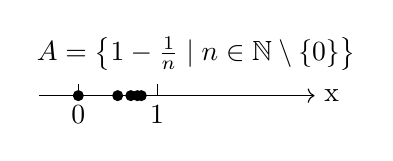
\begin{tikzpicture}

    % Disegno della retta dei numeri
    \draw[->] (-0.5,0) -- (3,0) node[right] {x}; % Freccia verso destra

    % Segna lo 0 con tacca corta
    \draw (0,0) node[below] {0} -- (0,0.15);  % Tacca e etichetta per 0
    
    % Segna l'1 con tacca corta
    \draw (1,0) node[below] {1} -- (1,0.15);  % Tacca e etichetta per 1

    % Disegno dei punti dell'insieme A
    % I punti 1 - 1/n per n = 1, 2, 3, 4, ...
    \foreach \n in {1, 2, 3, 4, 5} {
        \pgfmathsetmacro{\point}{1 - 1/\n}
        \fill (\point, 0) circle (2pt);  % Punti per A
    }

    % Etichetta per l'insieme A
    \node[above] at (1.5, 0.2) {$A = \left\{ 1 - \frac{1}{n} \mid n \in \mathbb{N} \setminus \{0\} \right\}$};

\end{tikzpicture}

\end{center}



\begin{center}
    \textbf{\textit{Definizione}}
\end{center}

\begin{itemize}
    \item Se $sup(A) \in A$, allora si chiama \textbf{\textit{massimo}} di $A$, indicato con $max(A)$
    \item Se $infa(A) \in A$, $inf(A) =min(A)$
\end{itemize}
In tal senso, il MASSIMO non esiste sempre, ma il $sup$ si
\\ Analogamente, il MINIMO non esiste sempre, ma l'$inf$ si.

\begin{center}
\textbf{\textit{Definizione}}
\end{center}
\begin{center}
    $sup \varnothing = -\infty$ \,\,\,\,\,\,\,\,\,\,\,\,\,\, $inf \varnothing = +\infty$
\end{center}

\begin{center}
\end{center}
\subsection{Teorema di caratterizzazione}
Considero $A\neq \varnothing, A \subset \mathbb{R}$ e suppongo $M(A) \neq \varnothing$, pongo inoltre $\alpha$ come $sup(A)$.
\\ Allora $\alpha$ soddisfa 2 proprietà:
\begin{enumerate}
    \item $\forall a \in A, \alpha \geqslant a$
    \item $\forall \varepsilon > 0, \exists \,\, a \in A$ tale che $\alpha < a+ \varepsilon$
\end{enumerate}
Viceversa dunque, se $\alpha$ rispetta queste due proprietà, allora $\alpha = sup(A)$
\begin{center}
    \textbf{\textit{Dimostrazione ($\Longrightarrow$)}}
\end{center}
Supponiamo che $\alpha=sup(A)$ rispetti sia 1. che 2.
\begin{enumerate}
    \item segue dal fatto che $\alpha \in M(A)$
    \item Vale per la dimostrazione che ne segue
\end{enumerate}
Se \underline{per assurdo} non fosse vera 2. allora $\exists \varepsilon>0$ tale che $\forall a \in A, \alpha \geqslant a + \varepsilon$.
\\ Se pongo adesso $\beta = \alpha - \varepsilon$ avrò un numero minore di $\alpha$ e che contemporaneamente appartiene a $M(A)$, ma ciò non è possibile, perchè $\alpha$ è il \underline{più piccolo} dei maggioranti, dunque la definizione è dimostrata per assurdo.
\begin{center}
   \#
\end{center}
\begin{center}
    \textbf{\textit{($\Longleftarrow$)}}
\end{center}
Supponiamo adesso che $\alpha \in \mathbb{R}$ soddisfi 1. e 2., allora voglio mostrare che $\alpha$ è $sup(A)$.
\\ Sicuramente $\alpha \in M(A)$ grazie alla proprietà 1.
\\ Inoltre, per la proprietà 2. so che $\forall \varepsilon>0, \exists a \in A$ tale che $\alpha-\varepsilon < a$.
\\
Supponiamo per assurdo che $\alpha \neq sup(A)$. Questo vuol dire che esiste allora un $\beta \in M(A)$ tale che $\beta < \alpha$.
\\ Sia adesso $\Bar{\varepsilon}=\frac{\alpha-\beta}{2}>0$. So dunque che $\exists a > \alpha - \varepsilon$, ma allora $a > \alpha - \frac{\alpha-\beta}{2}= \frac{\alpha}{2}+ \frac{\beta}{2}> \frac{\beta}{2}+ \frac{\beta}{2}=\beta$
\\ In sintesi, $a>\beta$, ma un elemento dell'insieme NON può essere più grande del \textbf{\textit{maggiorante}}.




\subsection{Principio/Assioma del minimo (nei naturali)}
Se $A \neq \varnothing$ e $A \subset \mathbb{N}$, allora $A$ ammette un minimo $inf(A)=min(A)$
\newpage
\subsection{Cenni di topologia di $\mathbb{R}$}
\subsubsection{Valore Assoluto}
Sia $x \in \mathbb{R}$, poniamo allora $|x|=\begin{cases}
    x \,\,\,\,\,\, \mbox{se} \,\,\,\,\,\, x \geqslant 0 \\ 
    -x \,\,\,\,\,\, \mbox{se} \,\,\,\,\,\, x \leqslant 0
\end{cases}$
\\
Il valore assoluto indica in senso stretto, e in valori positivi o nulli, la \underline{\textbf{distanza dall'origine}} di un numero.

\begin{center}
    \textbf{\textit{{Proprietà del valore assoluto}}}
\end{center}
\begin{enumerate}
    \item $|x| \geqslant0 \,\,\,\,\,\, \forall x \in \mathbb{R}$
    \item $|x| =0$ se e solo se ($\Longleftrightarrow$) $x=0$
    \item Sia $r >0$, allora $|x| \leqslant r \Longleftrightarrow -r \leqslant x \leqslant r$
    \item$ |x+y|\leqslant |x|+ |y|$, ossia la \textbf{\underline{disuguaglianza triangolare}}
    \item $|ab|=|a||b|$
    \end{enumerate}

\begin{center}
    \textbf{\textit{{Dimostrazione delle proprietà del Valore Assoluto}}}
\end{center}
\begin{itemize}
    \item 1 segue facilmente dalla definizione di valore assoluto
    \item 2 segue facilmente dalla definizione di valore assoluto
    \item 3, bisogna osservare la terza proprietà graficamente per poi poterla dimostrare:
    \begin{center}
   \LARGE$\Longrightarrow$
\end{center}

\begin{center}
\begin{tikzpicture}
    % Disegna la retta orizzontale
    \draw[->] (-4,0) -- (4,0);  % Frecce su entrambi i lati della retta

    % Disegna lo 0 al centro
    \draw[fill] (0,0) circle [radius=0.05];  % Punto
    \node[below] at (0,0) {$0$};  % Etichetta sotto

    % Disegna il punto r
    \draw[fill] (3,0) circle [radius=0.05];  % Punto
    \node[below] at (3,0) {$r$};  % Etichetta sotto

    % Disegna il punto -r
    \draw[fill] (-3,0) circle [radius=0.05];  % Punto
    \node[below] at (-3,0) {$-r$};  % Etichetta sotto

    % Disegna il punto x tra 0 e r
    \draw[fill] (1.5,0) circle [radius=0.05];  % Punto
    \node[below] at (1.5,0) {$x$};  % Etichetta sotto

\end{tikzpicture}
\end{center}
Ora, bisogna considerare i due casi, posto sempre che $|x| \leqslant r$:
\begin{itemize}
    \item Se $x \geqslant0$, allora $x \geqslant r$, ma $|x|=x$, per cui $a \leqslant r$, per cui, unendo le due condizioni, si ottiene che $-r \leqslant x \leqslant r$
    \item Se $x \leqslant 0$, allora $x \leqslant r$, ma $|x|=-x$, allora $x \geqslant -r$, da cui, unendo le due condizioni, si ha $-r \leqslant x \leqslant r$
\end{itemize}

\begin{center}
    \LARGE $\Longleftarrow$
\end{center}
Si dimostra ora il viceversa, ossia che, se $-r \leqslant x \leqslant r$, allora $|x| \leqslant r$.
\\
Considero sempre i due casi:
\begin{itemize}
    \item Se $x \geqslant 0$, $x=|x|\leqslant r$
    \item Se $x \leqslant 0$, $|x|=-x\leqslant r$, da cui $x \geqslant -r$, per cui $-r \leqslant x \leqslant r$
\end{itemize}
\newpage
\item 4, bisogna dimostrare la diseguaglianza triangolare:
\begin{center}
$|x+y| \leqslant |x|+|y|$
\end{center}
 Io so che $x \leqslant |x|$ e noto che, dato $|-x|=x \Longrightarrow \,\, x \geqslant -|x|$.
 \\ Ora osservo dunque che ho due condizioni:
 \begin{center}
     $-|x|\leqslant x \leqslant |x|$
     \\ $-|y| \leqslant y \leqslant |y|$
 \end{center}
Per cui, sommando membro a membro, ottengo una forma del tipo
\begin{center}
    $-(|x|+|y|) \leqslant x+y \leqslant |x|+|y|$
\end{center}
Definisco ora $|x|+|y|=r$, per cui avrò:
\begin{center}
    $-r \leqslant x+y \leqslant r$, ma allora
    $|x+y|\leqslant r \Longrightarrow |x+y| \leqslant |x|+ |y|$
\cvd
\end{center}
\item 5,Dimostriamo che $|ab|=|a||b|$:
\begin{itemize}
    \item Se $a>0$, $b>0$ vale che $|ab|=a \cdot b = |a||b|$
    \item Se $a<0$, $b<0$ vale che $|ab|= a \cdot b = |a| \cdot |b|$
    \item Se $a<0$, $b>0$ vale che $|ab| = -ab= (-a)(b)=|a| \cdot |b|$
    \item Se $a>0$, $b<0$ vale che $|ab|= -ab = (a)(-b)= |a| \cdot |b|$
\end{itemize}
\end{itemize}

\subsection{Notazioni su alcune proprietà e sottoinsiemi di $\mathbb{R}$}
\subsubsection{Definizione degli intervalli}
\begin{itemize}
    \item $A \subset \mathbb{R}$ è un insieme \textbf{connesso} se
    \begin{center}
        $\forall \,\, x,y \in A, \,\,\,\,\, z \in \mathbb{R}, \,\,\, x \leqslant z \leqslant y, \,\,\,\Longrightarrow  z \in A$
    \end{center}
    \item Un intervallo in $\R$ è un \underline{insieme connesso di $\mathbb{R}$}
\end{itemize}

\subsubsection{Caratterizzazione degli intervalli: intervalli aperti e chiusi}
$A \subset \mathbb{R}$ è un insieme \underline{aperto}:
\\
Se $\forall x \in A, \exists \,\, \varepsilon>0$ tale che $(x- \varepsilon, x+ \varepsilon) \subset A$
\\
$A$ insieme chiuso è l'insieme \textbf{\underline{complementare}} di uno aperto, dunque:
\\
$C=\mathbb{R}-A$

\subsection{Punti di accumulazione}
Sia $A \subset \mathbb{R}$, definisco $Acc(A) \subset \mathbb{R}$ l'insieme dei punti $x \in \mathbb{R}$ tali che $\forall \varepsilon > 0$, definisco inoltre l'insieme\\
$(x-\varepsilon; x+ \varepsilon) \cap A - \{x\} \neq \varnothing$, allora \underline{i punti di accumulazione $Acc(A)=[a;b]$}

\subsubsection{Insieme dei punti di aderenza}
Sia $A \subset \mathbb{R}$, allora l'insieme dei punti di aderenza è l'insieme di tutte le $x \in \mathbb{R}$ tali che $\forall \,\,\, \varepsilon > 0, A \cap (x- \varepsilon; x+ \varepsilon) \neq \varnothing$

\subsubsection{Insieme dei punti singolari}
L'insieme dei punti singolari è definito come:
\\ Insieme dei punti di aderenza (A)$-Acc(A)$
\begin{center}
    \textbf{\textit{Esempio}}
\end{center}
Consideriamo ad esempio l'insieme $X=\{x=\frac{1}{n} | n \in \N\}$, allora osserviamo che questo insieme ha un solo punto di accumulazione, ossia $0$, cioè il punto a cui tende la successione, e poi ha l'insieme dei punti di aderenza che corrisponde a tutti i punti dell'insieme (perchè se prendo le x dell'insieme, la loro intersezione con l'insieme non è vuota a prescindere da $\varepsilon$). Infine l'insieme dei punti singolari è l'insieme di tutti i punti dell'insieme tranne lo zero, è infatti esplicativo osservare come effettivamente ogni punto dell'insieme sia un punto \virgolette{separato dagli altri}. 
\begin{center}
    \textbf{\textit{Definizione}}
\end{center}
$K \subset \mathbb{R}$ è compatto se è chiuso e limitato (ossia se ha maggiorante e minorante)
\begin{center}
    $M(K) \neq \varnothing \neq m(K)$, dove
    \\ $M(K)$ è l'insieme dei maggioranti e $m(k)$ è l'insieme dei minoranti
\end{center}

\subsubsection{Alcune formule utili}

\begin{center}
    \textbf{\textit{Principio di Induzione}}
\end{center}
Per la dimostrazione della proprietà accennata sopra, è necessario il principio di induzione, utile per effettuare dimostrazioni in ambito logico-matematico.

Siano allora $P_1,P_2,P_3,...,P_n$ tutte proposizioni che dipendono da $n \in \mathbb{N}$.
Poniamo allora due ipotesi:
\begin{itemize}
    \item Supponiamo che $P_0$ sia \underline{vera}
\item $P_n$ vera $\Longrightarrow P_{n+1}$ vera, allora $P_n$ è vera $\forall n \in \mathbb{N}$
\end{itemize}
\begin{center}
    \textbf{\textit{Dimostrazione vera e propria}}
\end{center}
Pongo $S=\{n \in \mathbb{N} | P_n \mbox{è falsa}\}$, voglio dunque dimostrare che $S = \varnothing$
\\ Suppongo allora, \underline{per assurdo}, che $S \neq \varnothing$.
\\ Se così fosse, $S$ ammetterebbe un minimo $K=min(S), k \in \mathbb{N}$, perchè \underline{qualsiasi sottoinsieme di $\mathbb{N}$} ammette un minimo al suo interno.
\\
Dunque abbiamo che $K=0$ è vera, perciò $K \geqslant 1$.
\\
Abbiamo dunque che $P_{K-1}$ è vera, perchè il minimo $n$ per cui $P_n$ è falsa, quindi tutti gli $n < K$ devono essere tali che $P_n$ è vera, e così anche $K-1$.
\\
Per ipotesi però, abbiamo che $P_{K-1} \,\,\,\, \mbox{vera} \Longrightarrow P_K \,\,\,\,\,\, \mbox{vera}$, e dunque abbiamo che $P_K$ è sia vera che falsa (perchè abbiamo detto che $K \in S$) contemporaneamente, che è un assurdo.
\cvd

\begin{center}
    \textbf{\textit{Conseguenze}}
\end{center}
Dimostrato dunque il funzionamento dei principio di induzione, si hanno alcune conseguenze logiche, ad esempio, posto
\begin{equation}
   a_1+a_2+...+a_n = \sum^n_{k=1}a_k
\end{equation}
che sarà dunque la somma di $n$ numeri reali.
\\ Posso allora considerare
\begin{equation}
    \sum^n_{k=1}k=\frac{n(n+1)}{2}
\end{equation}
e dimostrare la sua veridicità attraverso una dimostrazione che sfrutta proprio il principio di induzione, osserviamo:
\begin{center}
    \textbf{\textit{Dimostrazione}}
\end{center}
Pongo $P_n=\sum^n_{k=1}k=\frac{n(n+1)}{2}$.
\\
\\$P_1$ è vera perchè $\frac{1(1+1)}{2}=1$, allora ciò che dobbiamo dimostrare ora è l'implicazione di verità da $P_n$ a $P_{n+1}$.
\\
\\
Considero $P_N=\sum^{n+1}_{k=1}k=\sum^{n}_{k=1}k + (n+1)=\frac{n(n+1)}{2}+(n+1)=\frac{n(n+1)+2(n+1)}{2}=\frac{(n+1)(n+2)}{2}$, il risultato dunque non è nient'altro che la formula da dimostrare ma con $(n+1)$ al posto di $n$.
\newpage
\begin{center}
    \textbf{\textit{Esercizio}}
\end{center}
Dimostrare che, anziché sommando k, sommando $k^2$, si ottiene che $\sum^{n}_{k=1}k^2=\frac{n(n+1)(2n+1)}{6}$.

\subsubsection{Somma geometrica}
Sia $q$ un numeri $q \in \mathbb{R}$, allora avrò che:
\\
\begin{center}
$\sum^{k=0}_{n}q^k=\frac{1-q^{n+1}}{1-q}$
\end{center}

\begin{center}
    \textbf{\textit{Dimostrazione}}
\end{center}
Poniamo $P_n: \sum^{k=0}_{n}q^k=\frac{1-q^k}{1-q}$
\\
$P_0$ è vera perchè $\sum_{k=0}^0 q^k =1=\frac{1-q^{0+1}}{1-q}=1$ ma ora bisogna verificare l'induzione $P_n \Longrightarrow P_{n+1}$.
\\
Considero 
\begin{center}
$\sum^{k=0}_{n+1}q^k=\sum^{k=0}_{n}q^k+q^{n+1}=\frac{1-q^{n+1}}{1-q}$.
\end{center}

Adesso, dalla somma
\begin{equation}
    \frac{1-q^{n+1}+q^{n+1}-q^{n+2}}{1-q}=\frac{1-q^{n+2}}{1-q}
\end{equation}
In questa maniera ho dimostrato che, anche nel caso della somma fino a $n+1$, la formula è valida comunque.

\subsubsection{Disuguaglianza di Bernoulli}
Sia $x \geqslant -1$.
\\ Sia invece $n \in \mathbb{N}$ \textbackslash $\{0\}$.
\\
Allora, per la \textit{disuguaglianza di Bernoulli}, vale
\begin{equation}
  P_n:  1+nx \leqslant (1+x)^n
\end{equation}
\begin{center}
    \textbf{\textit{Dimostrazione}}
\end{center}
$P_1$ è vera perchè ottengo $(1+x) \leqslant (1+x)$
\\
Verifichiamo adesso il caso \virgolette{$n+1$}:
\\
\begin{equation}
    (1+x)^{n+1}=(1+x)^n(1+x)
\end{equation}
Essendo vera l'equazione di sopra, allora abbiamo che
\begin{equation}
    (1+x)^n(1+x) \geqslant (1+nx)(1+x)
\end{equation}
da cui
\begin{equation}
    (1+x)^{n+1}\geqslant 1+x+nx+nx^2
\end{equation}
Adesso, siccome $n \in \mathbb{N}-\{0\}$ e $nx^2 \geqslant 0$, è possibile affermare come la disuguaglianza sia verificata eliminando $nx^2$, perchè:
\begin{equation}
    (1+x)^{n+1} \geqslant 1+ (1+n)x + nx^2 \geqslant 1+ (1+n)x
\end{equation}

\newpage
\section{Funzioni: generalità}
\begin{center}
    \textbf{\textit{Relazione}}
\end{center}
Dati due insiemi $X$ e $Y$, considero $X\times Y = \{(x,y) | \,\, x \in X, \,\,\,\, y \in Y\}$
\\
In sostanza, una \textbf{\textit{relazione}} tra i due insiemi è un \underline{sottoinsieme del prodotto cartesiano}
\\
\begin{center}
    \textbf{\textit{Funzione}}
\end{center}
Che cos'è una funzione?
\\
Una funzione è una relazione $f$ tale che se $(x,y_1)$ e $(x, y_2)$ sono $\in f$, allora $y_1=y_2$.
\\ Ciò vuol dire che a ogni elemento dell'insieme di partenza (\underline{dominio}), viene associato \underline{UNO E UN SOLO} $y$ corrispondente.
\\
La scrittura notazionale classica della funzione è
\begin{center}
   $ f: X \rightarrow Y$
    \\
    \,\,\,\,\, \,\,\,\,\,\,\,\,\,\,\,\,\,\,\,\,\,\small{$x \mapsto f(x)=y$}
\end{center}
\begin{center}
    \textbf{\textit{Osservazione}}
\end{center}
\begin{align*}
f \colon \mathbb{R} &\to \mathbb{R} \\
x &\mapsto x^2
\end{align*}

è diversa da \begin{align*}
g \colon [0;+\infty) &\to \mathbb{R} \\
x &\mapsto x^2
\end{align*}
Questo perchè quando si parla di una funzione, non bisogna soltanto considerare la relazione, ma anche dominio e codominio, quindi relazioni uguale ma con dominio differente sono funzioni differenti.
\begin{center}
    \textbf{\textit{Vocabolario}}
\end{center}
\begin{itemize}
    \item $R=A \times B$ è \textit{riflessiva} se $(a,a) \in R$
    \item  $R=A \times B$ è \textit{transitiva} se, qualora $(x,y) \in R$, allora $(y,z) \in R$
    \item $R=A \times B$ è \textit{simmetrica} se $(x,y) \in R \Longrightarrow$ $(y,x) \in R$
\end{itemize}
\subsection{Definizione di Insieme Immagine}
L'insieme immagine di $f$ è definito come:
\begin{equation}
    Im(f)=f(x)=\{y \in Y | \exists x \in X \mbox{tale che} f(x)=y\}
\end{equation}

\subsection{Definizione di Retroimmagine}
L'insieme \virgolette{retroimmagine} di $f$ è definito come (con $A \subset Y)$:
\begin{equation}
    f^{-1}(A)=\{x \in X | f(x) \in A\}
\end{equation}

\newpage
\subsection{Definizione di Funzione composta}
Consideriamo $X,Y,Z$ insiemi:
\\
\begin{center}
    $f: X \Rightarrow Y \,\,\,\,\,\,\,\,\,\,\,\,\,\, g: Y \Rightarrow Z$
\end{center}
La funzione $h=f \circ g$ ha una struttura del tipo:
 è diversa da \begin{align*}
g \colon X &\to Z \\
x &\mapsto g(f(x))
\end{align*}

\begin{center}
    % Questo è il testo che verrà visualizzato sulla pagina
    \textbf{Rappresentazione grafica della struttura di una funzione composta}

    \vspace{1cm} % Spazio verticale tra il testo e il diagramma

    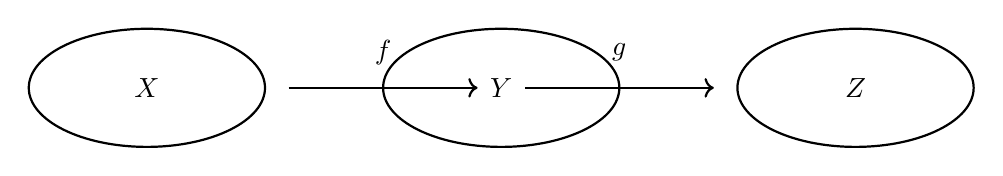
\begin{tikzpicture}[scale=1.5]

        % Disegna i tre insiemi ovali
        \draw[thick] (-3,0) ellipse (1 and 0.5);
        \draw[thick] (0,0)  ellipse (1 and 0.5);
        \draw[thick] (3,0)  ellipse (1 and 0.5);

        % Etichetta degli insiemi
        \node at (-3,0) {$X$};
        \node at (0,0) {$Y$};
        \node at (3,0) {$Z$};

        % Freccia da X a Y con etichetta "f"
        \draw[->, thick] (-1.8,0) -- (-0.2,0);
        \node at (-1, 0.3) {$f$};

        % Freccia da Z a Y con etichetta "g" (verso opposto)
        \draw[<-, thick] (1.8,0) -- (0.2,0);
        \node at (1, 0.3) {$g$};

    \end{tikzpicture}
\end{center}


\subsection{Funzioni Iniettive, Suriettive e Biettive}
\subsubsection{Iniettività}
Una funzione $f: X \rightarrow Y$ è iniettiva se:
\begin{center}
$\forall x_1,x_2 \in X, \,\,\,\,\,\,\, x_1\neq x_2 \Longrightarrow f(x_1) \neq f(x_2)$
\end{center}
oppure se
\begin{center}
    $f(x_1)=f(x_2) \Longrightarrow x_1=x_2$
\end{center}

\subsubsection{Suriettività}
Una funzione $f: X \rightarrow Y$ è suriettiva sa:
\begin{center}
    $Im(f)=Y$
\end{center}
oppure se 
\begin{center}
    $\forall y \in Y, \exists x \in X$ tale che $f(x)=y$
\end{center}
\subsection{Biettività}
Una funzione $f: X \rightarrow Y$ è biettiva se è sia iniettiva che suriettiva
\subsubsection{Funzione inversa}
Una funzione $f: X \rightarrow Y$ è detta \virgolette{invertibile} se $\exists g : Y \rightarrow X$ tale che $f(g(y))=y, \,\, \forall y\in Y$ e $g(f(x))=x, \,\, \forall x \in X$.
\\ Tale funzione prende il nome di \underline{funzione inversa}, e la sua notazione è
\begin{equation}
    f^{-1}
\end{equation}
\subsubsection{Invertibilità di una funzione}
\begin{center}
    \textbf{\textit{Teorema della funzione inversa}}
\end{center}
Il teorema della funzione inversa afferma che:
\\
Sia $f: X \rightarrow Y$ una funzione. Allora $f$ è invertibile $\Longleftrightarrow f$ è biettiva
\begin{center}
    \textbf{\textit{Dimostrazione}}
\end{center}
\begin{center}
    ($\Longrightarrow$)
\end{center}
Se $f(x_1)=f(x_2)$ con $x_1,x_2 \in X$, allora $g(f(x_1))=g(f(x_2))$ se $g$ è l'\textbf{inversa} della funzione $f$. Per cui la funzione $f$ è iniettiva.
\\
$f$ è allo stesso tempo \textbf{suriettiva}.
\\ Sia $y \in Y$, sia $g: Y \to X$ la funzione inversa di $f$.
Pongo allora $x=g(y) \in X$.
\\Ottengo allora $f(x)=f(g(y))=y$.
\\ Dunque $f$ è suriettiva, perchè la totalità dell'insieme delle immagini corrisponde con la totalità dell'insieme delle $y \in Y$, dove $Y$ rappresenta il codominio.
\begin{center}
    ($\Longleftarrow$)
\end{center}
Definiamo:
\begin{align*}
g \colon Y &\to X \\
y &\mapsto g(y)
\end{align*}
dove $g(y)= x \in X$ tale che $f(x)=y$.
\\
$g$ è ben definita perchè:
\begin{enumerate}
    \item se a $y \in Y$ potessi associare più di un valore di $x \in X$ tale che $f(x)=y$ ,allora la funzione $f$ NON SAREBBE INIETTIVA (assurdo)
    \item Tale $x$ inoltre, esiste perchè $f$ è \underline{suriettiva}
    \begin{center}
       Definita la funzione, verifichiamo il resto:
    \end{center}
    \item Controllo che $f(g(y))=y$
    \\ $g(y)$ è, per definizione, un elemento $x \in X$ tale che $f(x)=y$, dunque $f(g(y))=y$
    \item $g(f(x))=x$.
    \\ Ho posto dunque $y=f(x)$, allora $g(y)$ è, per definizione, l'elemento $x_0 \in X$ tale che $f(x_0)=y=f(x) \Longrightarrow x_0=x$ per \underline{iniettività}
\end{enumerate}
\begin{center}
    \#
\end{center}

\subsubsection{Esercizi utili}
\begin{enumerate}
    \item \begin{align*}
 X \to Y \to Z \\
\,\,\,\,\,\,\,\,\,\,\,x \mapsto f(x) \mapsto g(f(x))
\end{align*}
Se $f,g$ sono iniettive, allora anche $f \circ g$ deve esserlo 
\begin{center}
    \textbf{\textit{Dimostrazione}}
\end{center}
Se $x_1 \neq x_2$, allora $f(x_1) \neq f(x_2)$, e dunque $g(f(x_1)) \neq g(f(x_2))$, allora $f \circ g$ è iniettiva
\item Funzione composta di suriettive è suriettiva 
\begin{center}
    \textbf{\textit{Dimostrazione}}
\end{center}
Definiamo $f:X \to Y$ tale che $f(x) = y \in Y$, \\
$g: Y \to Z$ tale che $g(y)=z \in Z$.
\\
Allora so che:
\begin{center}
    $\forall y \in Y \,\,\, \exists x \in X$ tale che $f(x) = y \in Y$ \\
    $\forall z \in Z \,\,\, \exists y \in Y$ tale che $g(y)=z \in Z$.
\end{center}
Allora so che $\forall z \in Z \,\,\, \exists x \in X$ tale che $g(f(x))=z \in Z$, ossia tale che $f \circ g$ è una funzione suriettiva
\item Composizione di biettive è biettiva
\begin{center}
    \textbf{\textit{Dimostrazione}}
\end{center}
So che $f \circ g$ è iniettiva per 1. e suriettiva per 2., dunque so che è biettiva

\end{enumerate}


\subsection{Teorema di Cantor-Schroder-Bernstein}
\begin{center}
    \textbf{\textit{Enunciati}}
\end{center}
\begin{enumerate}
    \item Se $\exists f: X \rightarrow Y$ iniettiva, allora $\exists g: Y \rightarrow X$ suriettiva
    \item Se $\exists f: X \rightarrow Y$ iniettiva e esiste $g: Y \rightarrow X$ iniettiva, allora $\exists h: X \rightarrow Y$ biettiva
\end{enumerate}
\begin{center}
    \textbf{\textit{Dimostrazione}}
\end{center}
\begin{enumerate}
    \item Sia $f: X \to Y$ una funzione iniettiva, allora posso definire $g:Y \to X$ una funzione tale che $g(y)=x \in X$, tale che:
    \begin{itemize}
        \item Se $y \in Im(f)$, allora $g(y)=x$ con $x$ tale che $f(x)=y$ (la funzione è già suriettiva perchè ogni elemento di x ha immagine in $Y$, ma mancano alcuni elementi per $Y$)
        \item Se $y \in Y -\{Im(f)\}$, allora $g(y) = \overline{x} \in X$, dove $\overline{x}$ è un generico elemento di $X$
    \end{itemize}
    \item Per esercizio
\end{enumerate}




\newpage

\section{Cardinalità}
Conducendo un'attenta analisi degli insiemi numerici affrontati nelle pagine precedenti, si osserva come sono tutti insiemi numerici \underline{infiniti}. Tuttavia, il fatto che siano infiniti non vieta che un insieme possa essere più \virgolette{numeroso} di un altro.
\\ Questo ragionamento potrebbe apparire come un controsenso, perchè come sarebbe possibile che degli insiemi numerici, tutti infiniti, possano avere più elementi di un altro.
\\ Per dare questo tipo di risposte è stato creato il concetto di \textbf{\textit{cardinalità}}.
\begin{center}
    Definizione
\end{center}
La cardinalità, nella sua forma più \virgolette{innocente}, descrive il numero di elementi di un insieme.
\\ Questo va bene per insiemi finiti, ma nel momento in cui ci si approccia a insiemi infiniti il concetto di cardinalità diventa leggermente più complesso.
\\
\subsection{Insiemi finiti e infiniti}
\begin{enumerate}
    \item Un insieme è infinito se non è finito
    \item Un insieme $A$ è finito se è in \underline{biezione} con un altro insieme $I_n$, dove $I_n=\{1,2,3,...,n\}$
    \\ Diremo in tal caso che la \textbf{cardinalità} di $A$ è n.
    \begin{center}
        $\#A=n$
    \end{center}
\end{enumerate}
\begin{center}
    \textbf{\textit{Esercizio}}
\end{center}
\begin{enumerate}
    \item Se $n \neq m$, $I_n$ \underline{non} è in biezione con $I_m$
    \begin{center}
        \textbf{\textit{Dimostrazione}}
    \end{center}
    Se $n>m$, allora non può esistere un $\varphi : I_n \to I_m$ iniettiva, perchè per definizione di funzione devo associare un solo elemento per ogni n, dunque essendo $n>m$, dovrò associare ad almeno due elementi di $I_n$ lo stesso elemento di $I_m$, rendendo così la funzione non iniettiva.
    \\
    Se $n<m$, allora non può esistere una $\varphi: I_n \to I_m$ suriettiva, perchè, sempre per definizione di funzione, posso associare ad ogni elemento di $I_n$ un diverso elemento di $I_m$, ma non posso mai raggiungere tutti gli elementi di $I_m$ perchè dovrei annullare il fatto che $\varphi$ sia una funzione (assocerei ad un elemento di $I_n$ più elementi di $I_m$).
    \\
    Dunque, l'unico caso che permette l'esistenza di una biezione tra questi due insiemi è $n=m$
    \item $\mathbb{N}$ non è finito ($\#\mathbb{N}= \infty)$
    \begin{center}
        \textbf{\textit{Dimostrazione}}
    \end{center}
    $\N$ non è finito perchè, se lo fosse, potrei metterlo in biezione con un insieme $I_n$. Ma, al contempo, per la sua definizione, so che esiste sempre un elemento $n+1$, dunque potrei contemporaneamente metterlo in biezione con $I_{n+1}$.
    \\
    Avrei dunque una biezione tra $I_n$ e $I_{n+1}$, biezione impossibile per la dimostrazione precedente. Assurdo.
\end{enumerate}

\begin{center}
    \textbf{\textit{Definizioni}}
\end{center}
\begin{enumerate}
    \item Diremo che $\#A \leqslant \#B$ se esiste:
    \begin{center}
        $\varphi: A \to B$ iniettiva, oppure se esiste $\psi : B \to A$ suriettiva
    \end{center}

    \item Diremo che $\#A=\#B$ se ha 
        \begin{center}
            $\#A \leqslant \#B$ e $\#A \geqslant \#B$
        \end{center}
    \item Diremo che $\#A=\#B$ se $\exists \,\,\,\, y: A \to B$ che mette in biezione i due insiemi
    \end{enumerate}

    \begin{center}
        \textbf{\textit{Osservazione/Esercizio}}
    \end{center}
Se $A \subset B$ allora $\#A \leqslant \#B$, infatti
\begin{center}
   \,\,\,\,\,\,\,\,\,\,\,\,\,\,\,\,\,\,\,\,\,\,\,\,\,\,\,\,\,\,\,\,\,\,\,\,\,\,\,\,\,\,\,\,\,\,\,\,\,\,\,\,\,\,\,\,\, $\varphi: A \to B$ è ben definita e iniettiva
    \\ $a \mapsto a$
\end{center}

\begin{center}
    \textbf{\textit{Definizione}}
\end{center}
$\#A < \#B$ se $\#A \leqslant \#B$ ma NON è vero il viceversa, dunque:
\\ $\nexists \,\,\, \varphi : B \rightarrow A$ iniettiva.
\newpage
\subsection{Hotel di Cantor}
\begin{center}
    \textbf{\textit{Storia e spiegazione}}
\end{center}
Per spiegare la cardinalità è possibile prendere in considerazione l'esempio dell'Hotel di Cantor.
\\Il matematico Georg Cantor immaginò un hotel a stanze infinite, tante quante i \underline{numeri naturali} $\mathbb{N}$.
\\
Posto che tutte le camere, seppur infinite, risultino piene, all'arrivo di un nuovo ospite, l'hotel riesce comunque a trovare una stanza, definendo la funzione 
\begin{center}
   $ \varphi: \mathbb{N}\to \mathbb{N}-\{1\}$
    \\$ \,\, n \mapsto n+1$
\end{center}

Questo vuol dire allora che
\begin{center}
$\#\mathbb{N} \leqslant \#\mathbb{N}-1 \leqslant \# \mathbb{N}$
\end{center}
Questa disuguaglianza ha valore perchè di fatto $\mathbb{N}- \{1\} \subset \mathbb{N}$.

\begin{center}
    \textbf{\textit{Teorema 1}}
\end{center}
\begin{center}
    $\#\mathbb{N}=\mathbb{N}- \{1,2,3,...,k\}$
\end{center}
\begin{center}
    \textbf{\textit{Dimostrazione}}
\end{center}
Posto X come un insieme \underline{infinito}, allora $\exists Y \subsetneqq X, \exists \varphi: X \to Y$ è iniettiva.
Immaginiamo infatti l'ipotesi in cui arrivi un bus con $\mathbb{N}$ passeggeri all'hotel, allora va definita la funzione
\begin{center}
    $\varphi : \mathbb{N} \to 2\mathbb{N}$
    \\ \,\,\,\,\,\,\, $n \mapsto 2n$
\end{center}
Questa $\varphi$ è di fatto iniettiva, perchè presi un $n\neq m$, si ha che $2n \neq 2m$.


\begin{center}
\textbf{\textit{Teorema 2}} 
\end{center}
\begin{center}
    $\#\mathbb{N}=\#\mathbb{Z}$
\end{center}
\begin{center}
    \textbf{\textit{Osservo (??)}}
\end{center}
Osservo che posso definire:
\begin{center}
    $\psi: \mathbb{N} \to \mathbb{Z}$ tale che
    \\
        $\psi(n)= \left\{\begin{array}{cc}
      \frac{n}{2}   & \mbox{se n è pari} \\
       \frac{n+1}{2}(-1)  & \mbox{se n è dispari}
    \end{array} \right.  $
\end{center}

tale per cui definisco gli \underline{interi} dai naturali e genero dunque una funzione \textbf{\underline{biettiva}}
\\
Se adesso immaginiamo l'arrivo di $\mathbb{N}$ autobus con $\mathbb{N}$ passeggeri ciascuno, tali che possiamo identificare ogni passeggero con una coppia di numeri $n,m$ dove troviamo l'$n$-esimo passeggero per l'$m$-esimo autobus.
\\
Associo allora l'identificazione del passeggero a $\mathbb{N} \times \mathbb{N}$.
\\
Si sa che $\#\mathbb{N} \subset \# (\mathbb{N} \times \mathbb{N})$, dunque
\begin{center}
    $\varphi: \mathbb{N} \times \mathbb{N} \to \mathbb{N}$
    \\ \,\,\,\,\,\,\,\,\,\,$(n,m) \mapsto n$
\end{center}


\newpage
Essendo $\varphi$ una funzione suriettiva (se scambio dominio e codominio diventa suriettiva), posso considerare $\varphi': (n,m) \to n^m$, che è iniettiva. \'E noto allora che $\#\mathbb{N} \times \mathbb{N} = \#\mathbb{N}$
\begin{center}
    \textbf{\textit{Osservazione}}
\end{center}
la funzione tale che $(n,m) \mapsto \frac{n}{m}$ è suriettiva da $\mathbb{N} \times \mathbb{N} $ \,\,in $\mathbb{Q_+}-\{0\}$.
Questo vuol dire che 
\begin{center}
    $\#\mathbb{N} \times \mathbb{N} \geqslant \#\mathbb{Q}$
\end{center}

\begin{center}
    \textbf{\textit{Osservazioni finali}}
\end{center}
Si osservi come $\#(\mathbb{N} \times \mathbb{N})=\#(\mathbb{Z} \times \mathbb{Z})$, ma $\mathbb{Z} \times \mathbb{Z}-\{0\}$ è in biezione con $\mathbb{Q}$.
\\ Dunque, in conclusione
$\#\mathbb{Q}=\#\mathbb{N}=\#\mathbb{Z}$

\subsection{Insieme delle parti e Aleph}
\begin{center}
    \textbf{\textit{Definizione}}
\end{center}
Definisco con $P(X)$ \underline{l'insieme dei sottoinsiemi} di X, ossia l' \virgolette{insieme delle parti} di X. \'E allora noto che $\#P(X)=2^n=2^{\#X}$ (si dimostra per induzione)
\begin{center}
    \textbf{\textit{Definizione}}
\end{center}
$\#\mathbb{N}=\aleph_0$
\begin{center}
    \textbf{\textit{Teorema}}
\end{center}
$\#X < \#P(X)$
\begin{center}
    \textbf{\textit{Dimostrazione}}
\end{center}
Definiamo una funzione INIETTIVA tale che:
\begin{center}
    $\varphi : X \to P(X)$
    \\  \,\,\,\,\,\,\,\,\, \,\,\,\,\,\,\, $x \mapsto \{x\}$ (insieme)
\end{center}
Supponiamo allora, per assurdo, che esista una funzione $\varphi: X \to P(X)$ suriettiva.
\\ Definiamo inoltre un insieme $A=\{x \in X | x \notin \varphi(x)\}$.
\\
Per il teorema di Schroder-Bernstein-Cantor si ha che:
\begin{center}
    Se $\exists \,\,\, \varphi_1 : P(X) \to X$ iniettiva, allora
    \\
    $\exists \,\,\, \varphi_2 :  X \to P(X)$ suriettiva
\end{center}
Allora $A=\{x \in X | x \notin \varphi(x)\} \in P(X)$
\\
Adesso, per la suriettività della funzione $\varphi_2$ è noto che $\exists \,\,\, a \in X$ tale che $A=\varphi(a)$.
\\
Ora la domanda è, $a \in A$ ??.
\begin{itemize}
    \item Se $a \in A$, allora avremo che $A = \varphi(a)$, ma in $A$ stanno tutte le $x$ tali che $x \notin \varphi(x)$, dunque si giungerebbe ad un assurdo
    \item Se $a \notin A$, allora $a \notin \varphi(a) \Rightarrow a \in A$, ma anche in questo caso siamo giunti ad un assurdo
\end{itemize}
Dunque, visti i due unici e possibili casi di appartenenza dell'elemento $a$ all'insieme $A$, e appurato che in entrambi si giunge ad un assurdo, la tesi è dimostrata.
\newpage
\begin{center}
    \textbf{\textit{Definizione}}
\end{center}
$\#P(\mathbb{N})=2^{\aleph_0}=\aleph_1$
\\
Esistono infiniti aleph ($\aleph_1,\aleph_2,...)$
\\
\subsubsection{Cardinalità del continuo e conclusioni}
Si dice inoltre che $\mathbb{R}$ abbia la \textbf{\underline{cardinalità del continuo}}, mentre $\mathbb{N}$ ha la cardinalità del discreto.
In sostanza, $\mathbb{R}$, essendo continuo, ha una cardinalità maggiore degli insiemi discreti (anche se infiniti), come $\mathbb{N}$, proprio a causa della continuità dei valori, che insiemi numerabili non hanno.
\\

Abbiamo dunque visto due tipi di \textbf{cardinalità}, quella del \textit{discreto} e quella del \textit{continuo}, ma ne esistono molte altre, basti pensare soltanto all'insieme dei sottoinsiemi di $\mathbb{R}$, e così via, a generare cardinalità sempre di ordine maggiore.

\subsubsection{Proposizione: $\#\R > \#\N$}
Vogliamo dimostrare che non esiste nessuna biezione tra $\R$ e $\N$
\begin{center}
    \textbf{\textit{Dimostrazione}}
\end{center}
Diagonale di Cantor:
\\
Assumiamo che i numeri $x \in \R | 0 < x < 1$ si possano porre in biezione con $\N$.
\\
Allora scrivo:
\begin{align*}
    x_1=0,a_1a_{1,1}a_{1,2}a_{1,3}a_{1,4}... \\
     x_2=0,a_1a_{2,1}a_{2,2}a_{2,3}a_{2,4}...\\
      x_3=0,a_1a_{3,1}a_{3,2}a_{3,3}a_{3,4}...\\
       ...
\end{align*}
Allora ho una lista infinita di numeri che è messa in biezione con $\N$. PER\'O osservo che posso sempre trovare un elemento che non appartiene a questa lista, ad esempio aggiungendo +1 sulla diagonale di questi numeri (per una spiegazione più precisa vedere qui : \\\url{https://it.wikipedia.org/wiki/Argomento_diagonale_di_Cantor#:~:text=L'argomento%20diagonale%20di%20Cantor,e%20della%20teoria%20della%20calcolabilit%C3%A0.}
\newpage
\section{Funzioni reali e altro}
\subsection{Funzioni reali}
Una funzione reale è una funzione nella forma:
\begin{center}
    $f: A \to \mathbb{R}, A \subset \mathbb{R}$
\end{center}
La funzione è definita solamente dove ha senso chiaramente, dunque nel suo \underline{dominio massimale}.

\subsection{Grafico di una funzione}
Definita
\begin{center}
    $f: X \to Y$
\end{center}
allora Graf($f$)$= \Gamma(f)=\{(x,y) \in X \times Y | y=f(x)\}$

\subsection{Monotonie}
La monotonia vale SOLO nelle $f$ reali, dunque:
\begin{itemize}
\item $f$ è \textbf{monotona crescente} se $\forall x_1,x_2 \in \mathbb{R}, x_1< x_2, f(x_1) \leqslant  f(x_2)$
    \item 
$f$ è \textbf{monotona strettamente crescente} se $\forall x_1,x_2 \in \mathbb{R}, x_1< x_2, f(x_1) <  f(x_2)$
\item $f$ è \textbf{monotona decrescente} se $\forall x_1,x_2 \in \mathbb{R}, x_1< x_2, f(x_1) \geqslant  f(x_2)$
\item $f$ è \textbf{monotona strettamente decrescente} se $\forall x_1,x_2 \in \mathbb{R}, x_1< x_2, f(x_1) >  f(x_2)$
\end{itemize}
\begin{center}
    \textbf{\textit{Proposizione}}
\end{center}
Sia $f: \mathbb{R} \to \mathbb{R}$.
\\ Se $f$ è \underline{strettamente monotona}, allora $f$ è invertibile nella sua immagine.
\begin{center}
    \textbf{\textit{Dimostrazione}}
\end{center}
Osserviamo subito che, se considero $f: \mathbb{R} \to Im(f)$, questa è una funzione, per costruzione, \textbf{suriettiva}.
\\ Ma se $x \neq y$ e $x<y$, allora $f(x)<f(y) \Rightarrow f(x) \neq f(y) \Rightarrow f$ è iniettiva.
\\ Essendo a questo punto \textbf{biettiva}, per il teorema della funzione inversa, la funzione $f$ è invertibile.
[ATTENZIONE! NON VALE IL VICEVERSA DI QUESTA PROPOSIZIONE].
\\
 Di fatto, non è che se una funzione qualsiasi è biettiva allora è invertibile, basta infatti pensare al caso di una funzione discontinua e questo viceversa crolla immediatamente.
\subsection{Una funzione strettamente crescente è invertibile con la stessa monotonia}
Sia $f:\R \to \R$ una funzione crescente, allora, per $x_1 < x_2$, $f(x_1)< f(x_2)$. Dunque adesso considero $g=f^{-1}$, e osservo che, presi $f(x_1) < f(x_2)$, allora $g(f(x_1))=x_1 < g(f(x_2))=x_2$ per ipotesi ($f$ crescente)
 
\subsection{Simmetrie}
\begin{itemize}
    \item $f$ è \underline{pari} se $f(-x)=f(x), \forall x \in D(f)$, quindi c'è una simmetria rispetto all'asse $y$
    \item $f$ è \underline{dispari} se $f(-x)=-f(x)$, dunque se c'è una simmetria rispetto all'\textbf{origine}.
\end{itemize}
    \subsection{Periodicità}
$f$ è periodica se $\exists \,\, T>0$ tale che $f(x+T)=f(x), \forall x \in \mathbb{R}$

\subsection{Inversa e grafico di un'inversa}
Se $(a,b) \in \Gamma (f^{-1}) \,\, \Longrightarrow (a,f^{-1}(a))$, ma se $a=f(x)$ (e posso trovare tale $x$ perchè per come è definita $f $ è suriettiva), allora ho $(f(x),f^{-1}(f(x)))=(f(x),x)$
\\
Graficamente avrò che, se $(a,b) \in \Gamma(f)$, allora $(a,b)$ e $(b,a)$ sono simmetrici rispetto a $y=x$
\begin{center}
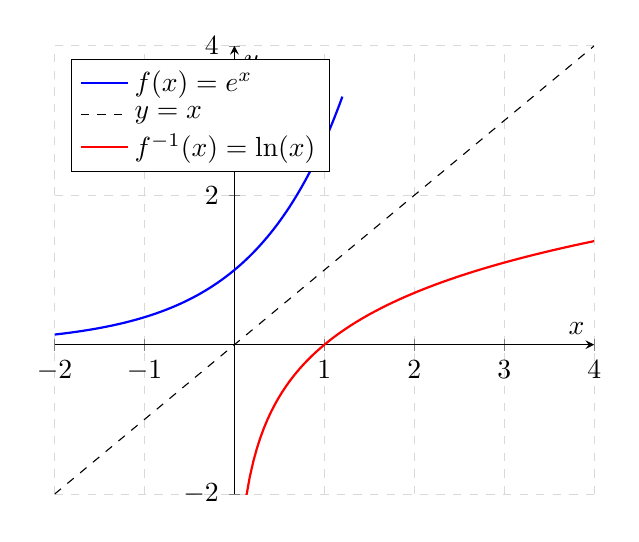
\begin{tikzpicture}
    \begin{axis}[
        axis lines = center,
        xlabel = \(x\),
        ylabel = \(y\),
        xmin = -2, xmax = 4,
        ymin = -2, ymax = 4,
        grid = both,
        grid style = {dashed, gray!30},
        legend pos = north west,
        legend cell align = {left},
    ]

    % Funzione f(x) = e^x (esempio di funzione invertibile)
    \addplot [
        domain=-2:1.2,
        samples=100,
        thick,
        blue,
    ] {exp(x)};
    \addlegendentry{\( f(x) = e^x \)}

    % Retta y = x (linea tratteggiata nera)
    \addplot [
        domain=-2:4,
        samples=2,
        dashed,
        black,
    ] {x};
    \addlegendentry{\( y = x \)}

    % Funzione inversa f^{-1}(x) = ln(x) (in rosso)
    \addplot [
        domain=0.05:4,
        samples=100,
        thick,
        red,
    ] {ln(x)};
    \addlegendentry{\( f^{-1}(x) = \ln(x) \)}

    \end{axis}
\end{tikzpicture}
\end{center}

\section{Trigonometria in breve}
\subsection{Basi della trigonometria (skippate)}
\subsection{Funzioni iperboliche}
Abbiamo due principali funzioni iperboliche, che sono:
\begin{equation}
    \sinh(x)=\frac{e^x-e^{-x}}{2} \,\,\,\,\,\,\, \mbox{xhe è una funzione dispari}
\end{equation}
\begin{equation}
    \cosh(x)=\frac{e^x+e^{-x}}{2}\,\,\,\,\,\,\,\, \mbox{che è una funzione pari}
\end{equation}
\begin{equation}
    tgh(x)=\frac{\sinh(x)}{\cosh(x)}
\end{equation}
Esiste, parallelamente alla relazione fondamentale della trigonometria, una relazione tale per cui vale
\begin{equation}
    \cosh^2(x)=1+\sinh^2(x)
\end{equation}
\subsection{Parte intera}
Definiamo la funzione parte intera come
\begin{equation}
    \lfloor x \rfloor = max\left\{n \in \mathbb{Z} \,\,\, | \,\,\, x \geqslant n\right\}
\end{equation}
Grafico qui: \url{https://upload.wikimedia.org/wikipedia/commons/e/e1/Floor_function.svg}


\subsection{Parte frazionaria}
La parte frazionaria è definita come:
\begin{equation}
    \{x\}=x-\lfloor x \rfloor 
\end{equation}
Grafico qui: \url{https://images.treccani.it/ext-tool/intra/images/8/8c/Enciclopedia_della_Matematica_fig_lettf_04600_001.jpg}


\newpage
\section{Successioni numeriche}
\subsection{Definizione}
Una successione è una \underline{funzione} tale che
\begin{center}
$f: \mathbb{N} \to \mathbb{R}$
\\\,\,\,\,\,\,\,\,\,\, $n \mapsto a_n$
\end{center}
\subsection{Limitazioni}
Una successione può essere limitata:
\begin{itemize}
    \item Inferiormente, se $\exists \,\,\, m$ tale che $a_n>m  \,\,\,\,\,\, \forall \,\,\,\,\, n \in \mathbb{N}$
    \item Superiormente se $\exists \,\,\, M$ tale che $a_n<M \,\,\,\, \forall \,\,\,\, n \in \mathbb{N}$
    \item Limitata e basta se esistono contemporaneamente $m,M$ tali che $m<a_n<M \forall n \in \mathbb{N}$
\end{itemize}
\subsection{Limite di successione finita}
Diremo che una successione {$a_n$} tende a un valore $l \in \mathbb{R}$, e dunque scriveremo 
\begin{center}
    $a_n \to l$
    \\ $n \mapsto +\infty$
\end{center}
oppure $\lim_{n \to +\infty}a_n=l$ se:
\begin{center}
    $\forall \,\, \varepsilon > 0 \,\,\, \exists \,\,\,\, N>0$ tale che, se $n>N$, allora $|a_n-l|<\varepsilon$
\end{center}
\begin{center}
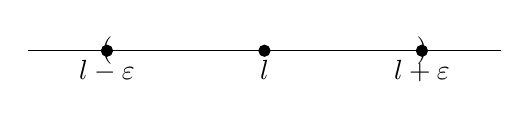
\begin{tikzpicture}

% Disegno della retta orizzontale
\draw[thin] (-3,0) -- (3,0);

% Posizioni dei punti l - \varepsilon, l, l + \varepsilon
\coordinate (A) at (-2,0);
\coordinate (B) at (0,0);
\coordinate (C) at (2,0);

% Disegno dei punti sulla retta
\filldraw (A) circle (2pt) node[below] {$l-\varepsilon$};
\filldraw (B) circle (2pt) node[below] {$l$};
\filldraw (C) circle (2pt) node[below] {$l+\varepsilon$};

% Parentesi tonda verso destra in corrispondenza di l - \varepsilon
\node at (-2,0.0) {$($};

% Parentesi tonda verso sinistra in corrispondenza di l + \varepsilon
\node at (2,0.0) {$)$};

\end{tikzpicture}
\end{center}
\subsection{Risultati teorici preliminari}
\begin{center}
    \textbf{\textit{Lemma utile (se e solo se)}}
\end{center}
Sia $a_n$ una successione tale che $a_n \to l\in \mathbb{R}$.
\\
Allora sono equivalenti:
\begin{enumerate}
    \item $a_n \to l$ ($a_n$ tende ad $l$)
    \item $\exists \,\,\, c>0, \,\,\, \forall \,\,\, \varepsilon>0$ (con $n>N$) tale che $|a_n-l|<c\varepsilon$
\end{enumerate}
\begin{center}
    \textbf{\textit{Dimostrazione del Lemma}}
\end{center}
\begin{center}
    \textbf{\textit{Da 1. a 2.}}
\end{center}
Ponendo c=1 ottengo la forma 2. dalla forma 1. semplicemente esplicitando il limite.
\begin{center}
    \textbf{\textit{Da 2. a 1.}}
\end{center}
Fissiamo $\varepsilon$, a questo punto cerco un $N>0$ tale che $n>N \Rightarrow |a_n-l|<(\frac{\varepsilon}{c})c$.
\\
Pongo dunque $\Bar{\varepsilon}=\frac{\varepsilon}{c}$ e dunque, esplicitando, ottengo che $\exists \,\,\, N>0$ tale che, se $n>N$, allora $|a_n-l|<c\Bar{\varepsilon}=\varepsilon$

\newpage
\begin{center}
    \textbf{\textit{Lemma 2}}
\end{center}
$a_n \to 0 \Longleftrightarrow |a_n| \to 0$.
\\
Esplicitiamo prima uno e poi l'altro:
\begin{center}
    $\forall \,\,\, \varepsilon>0, \,\, \exists \,\,\, N>0$ tale che, se $n>N$, allora $|a_n-l|<\varepsilon$
\end{center}
e
\begin{center}
    $\forall \,\,\, \varepsilon>0, \,\, \exists \,\,\, N>0$ tale che, se $n>N$, allora $||a_n|-0|<\varepsilon$, ma $||a_n||=|a_n|$
\end{center}
Dunque sono uguali, e questo è un risultato abbastanza importante, perchè ci permette di capire come \\
\underline{il valore assoluto di una successione} tende allo zero in maniera uguale alla successione stessa.

\subsection{Unicità del limite}
\begin{center}
    \textbf{\textit{Proposizione}}
\end{center}
Sia $a_n$ una successione.
\\
Supponiamo che $a_n \to l \in \mathbb{R}$ e $a_n \to m \in \mathbb{R}$, allora $l=m$
.
\begin{center}
    \textbf{\textit{Dimostrazione diretta}}
\end{center}
considero il valore $0 \leqslant|l-m|=|l-a_n+a_n-m|$
.
\\ Utilizzo allora la \textit{disuguaglianza triangolare}, per cui
\begin{center}
    $|l-a_n+a_n-m| \leqslant |l-a_n|+|a_n-m|$
\end{center}
Sia $|l-a_n|$ che $|a_n-m|$ risulteranno $< \frac{\varepsilon}{2}$ da un certo $N$(diverso per i due casi) in poi.
\\
Dato allora che $a_n \to l$, esplicito il limite:
\begin{center}
    $\forall \,\,\, \varepsilon >0, \,\,\, \exists \,\,\, N_1>0$ tale che, se $n>N$, allora $|a_n-l|< \frac{\varepsilon}{2}$.
\end{center}
Analogamente è noto che, dato $a_n \to m$, allora avrò:
\begin{center}
    $\forall \,\,\, \varepsilon>0, \,\,\, \exists N>0$ tale che, se $n>N$, allora $|a_n-m|<\frac{\varepsilon}{2}$
\end{center}
Scelgo allora una $N$ che vada bene a entrambi, come ad esempio la somma tra $N_1$ e $N_2$ o il loro prodotto.
\\
Scelto dunque $N>N_1+N_2$ oppure $N=max\{N_1;N_2\}$, troverò che, per $n>N$, tornando alla disuguaglianza triangolare, avrò:
\begin{center}
    $|l-m|=|l-a_n+a_n-m| \leqslant |l-a_n|+|a_n-m|$
\end{center}
Dai limiti precedentemente esplicitati è inoltre noto che, singolarmente:
\begin{center}
    $|a_n-l|<\frac{\varepsilon}{2}$ e \,\,\,\,\,\,\,\,\,\,\,\,\,\,\, $|m-a_n|<\frac{\varepsilon}{2}$
\end{center}
Per cui si ha che
\begin{center}
    $|l-m|\leqslant |l-a_n|+|a_n-m| \leqslant \frac{\varepsilon}{2}+ \frac{\varepsilon}{2}= \varepsilon$
\end{center}
Scelto però un $\varepsilon \to 0$, si avrà $|l-m|=0$, dunque $l=m$
\subsection{Limite infinito di una successione}
\begin{center}
    \textbf{\textit{Definizione}}
\end{center}
Diremo che $a_n$ \underline{diverge} a $+\infty$ oppure a $-\infty$ o anche che \underline{tende} a $+\infty,-\infty$ se:
\\
\begin{center}
    $\forall \,\,\, M>0 \,\,\, \exists \,\,\, n>M$ tale che $a_n>M$
\end{center}
Per il limite che tende a $-\infty$ invece diventa:
\begin{center}
    $\forall \,\,\, M>0 \,\,\, \exists \,\,\, n>M$ tale che $a_n<-M$
\end{center}

\newpage
\subsection{Proprietà delle successioni}
\begin{center}
\textbf{\textit{Definizione}}
\end{center}
[Questa è una definizione rischiosa]
\\
Se una successione possiede una determinata proprietà $P_n$, e questa proprietà si manifesta soltanto da un certo valore di $n$ in poi, allora diremo che questa proprietà si verifica \virgolette{\underline{definitivamente}}.
\\
Cioè, d'ora in poi, quando verrà usato il termine \virgolette{\underline{definitivamente}}, bisognerà intendere come un \virgolette{da un certo $n > 0 $ in poi si verifica una determinata proprietà}.
    


\begin{center}
\textbf{\textit{Definizione}}
\end{center}

    Se una successione $a_n \longrightarrow 0$, diremo che $a_n$ è \virgolette{infinitesima}.
\begin{center}
\textbf{\textit{Lemma utile}}
\end{center}
    Siano $\{a_n,b_n\}$ successioni numeriche tali per cui $a_n$ è \textbf{infinitesima} e $b_n$ è limitata.
    \\
    Intendiamo dunque dire che $a_n \longrightarrow 0$ e che $|b_n|< c$, con $c \in \mathbb{R}, \,\,\, \forall \,\,\, n \in \mathbb{N}$.
    \\
    Allora, il prodotto delle successioni $a_nb_n$ è una successione anch'essa infinitesima.
\begin{proof}
    Sia $\varepsilon>0$, allora è noto che $|a_nb_n|\leqslant|a_n|c< \varepsilon$ \virgolette{definitivamente}
\end{proof}
\begin{center}
\textbf{\textit{Esempio}}
\end{center}

    Ad esempio, la successione $\frac{(-1)^n}{n}\to0$, perché $(-1)^n$ è limitata e $\frac{1}{n}$ è infinitesima
\begin{center}
\textbf{\textit{Esempio}}
\end{center}

    $\frac{1}{n^2} \to 0$, perchè $\frac{1}{n}$ è limitata (0) e $\frac{1}{n}$ è infinitesima.
\begin{center}
\textbf{\textit{Proposizione}}
\end{center}

    Sia $a_n$ una successione tale che $a_n \to a$, con $a \in \widetilde{\mathbb{R}}$.
    \\
    Allora si avrà che:
    \begin{enumerate}
        \item $e^{a_n} \to \begin{array}{ccc}
         0    & \mbox{se} & a=-\infty \\
          e^a   & \mbox{se} & a \in \mathbb{R} \\
            +\infty & \mbox{se} & a=+\infty
        \end{array}$
        \item (con $a \geqslant 0$), $ln(a_n) \to \begin{array}{ccc}
            -\infty & \mbox{se}& a=0 \\
            ln(a) & \mbox{se}& a \in \mathbb{R}\\
            +\infty & \mbox{se}& a=+\infty
        \end{array}$
    \end{enumerate}
\begin{center}
\textbf{\textit{Dimostrazione parziale, solo di due casi}}
\end{center}
\begin{itemize}
    \item Caso 1.
    \\
    \hl{Dimostriamo che $ln(a_n) \to -\infty$ se $a_n \to 0$, con $a_n > 0$}:
    \\
    Voglio mostrare che, per $M>0$, allora $ln(a_n) < -M$.
    \\
    Dunque $\exists$ $N>0$ tale che, se $n>N$, $ln(a_n)<-M$.
    \\
    Ora, $ln(a_n)<-M$, per la stretta crescenza dell'esponenziale, che permette di mantenere reale la disuguaglianza, sarà uguale a $a_n<e^{-M}$.
    \\
    Pongo $\varepsilon = e^{-M}>0 $, e questo è proprio il valore $\varepsilon>0$ che cercavamo, dunque possiamo dire che $\exists$ $N>0$ tale che, se $n>N$, allora $a_n<\varepsilon$
\item Caso 2.
\\
\hl{Dimostriamo che $e^{a_n} \to e^a$ se $a_n \to a$, con $a \in \mathbb{R}$}
\\
Fisso un generico $\varepsilon>0$.
\\
Mi chiedo se, \virgolette{definitivamente}, $|e^{a_n}-e^a|<\varepsilon$.
Dall'ultima disequazione si arriva a 
\begin{center}
    $e^a|e^{a_n-a}-1|<\varepsilon$, da cui $|e^{a_n-a}-1|<\varepsilon e^{-a}$, ossia
    \\
    $ 1- \varepsilon e^{-a} < e^{a_n-a} <1+ \varepsilon e^{-a}$.

    
\end{center}
Ora, se $1- \varepsilon e^{-a}<0$, la disuguaglianza di sinistra è ovvia, altrimenti si ha, passando al logaritmo (che abbiamo visto mantenere vere le disuguaglianze):
\begin{center}
    $ln(1- \varepsilon e^{-a})<a_n-a<ln(1+ \varepsilon e^{-a})$
\end{center}
Definisco $-\alpha_-$ il logaritmo di sinistra, mentre definisco $\alpha_+$ il logaritmo di destra.
\\
Pongo $\overline{\varepsilon}=min\{\alpha_+;\alpha_-\}>0$.
\\
Dunque su che $\exists$ $N>0$ tale che, se $n>N$ si ha $|a_n-a|<\varepsilon$, ossia che
\begin{center}
    $-\alpha_- \leqslant -\overline{\varepsilon} < a_n-a < \overline{\varepsilon} \leqslant \alpha_+$
\end{center}
\end{itemize}
\newpage
\section{Algebra dei limiti}
\subsection{Algebra dei limiti \underline{finiti}}
Supponiamo che esistano due successioni $a_n \longrightarrow a$ e $b_n \longrightarrow b$, con $a,b \in \mathbb{R}$
\\
Allora valgono le seguenti proprietà:
\begin{enumerate}
    \item $a_n \pm b_n \longrightarrow a \pm b$
    \item $a_nb_n \longrightarrow ab$
    \item $\frac{a_n}{b_n} \longrightarrow \frac{a}{b}$ se $b_n \neq 0 \,\,\, \forall \,\,\, n$
\end{enumerate}
\begin{proof}
\begin{itemize}
    \item Caso 1.
    \\
    Fisso un generico $\varepsilon>0$ e cerco un $n>0$ tale che, se $n>N$, allora
    \begin{center}
        $|a_n+b_n-(a+b)|<\varepsilon$
    \end{center}
Osservo dunque che $|a_n+b_n-(a+b)|=|(a_n-a)+(b_n-b)|$ e che, per la disuguaglianza triangolare:
\begin{center}
    $|(a_n-a)+(b_n-b)|\leqslant |a_n-a|+|b_n-b|$
\end{center}
E' allora noto che, esplicitando separatamente i due limiti, si ha
\\
Che $\exists$ $N_1>0$ tale che $|a_n-a|<\frac{\varepsilon}{2}$
\\
Che $\exists$ $N_2>0$ tale che $|b_n-b|<\frac{\varepsilon}{2}$
\\
Dunque, se considero per entrambi un $N=max\{N_1,N_2\}$, avrò che, in entrambi i casi, per $n>N$, varrà la disuguaglianza:
\begin{center}
    $|a_n+b_n|\leqslant \frac{\varepsilon}{2}+\frac{\varepsilon}{2}=\varepsilon$
\end{center}
\item Caso 2.
\\
Fisso $\varepsilon>0$ e cerco un $N>0$ tale che $|a_bb_n|< \varepsilon$.\\
Allora considero che
\begin{center}
    $||a_nb_n-ab|=|a_nb_n-ab_n+ab_n-ab|=|b_n(a_n-a)+a(b_n-b)|$
\end{center}
Che, utilizzando la disuguaglianza triangolare, diventa
\begin{center}
    $|b_n(a_n-a)+a(b_n-b)|\leqslant |b_n||(a_n-a)|+|a||(b_n-b)|$
\end{center}
Considero il fatto che
\begin{center}
    $\forall \,\,\, \varepsilon>0 \,\,\, \exists \,\,\, N>0$ tale che, se $n>N$, allora $|b_n-b|<\varepsilon$
\end{center}
Considerato ciò, so che
\begin{center}
    $|a||b_n-b|\leqslant|a|\varepsilon$
\end{center}
Ora andiamo al secondo termine:
\\
Bisogna tenere conto del fatto che, se una successione tende ad un numero, allora, \underline{definitivamente}, quella successione sarà limitata, compresa tra due valori da cui non può scappare, perchè tende a qualcosa.
\\
In questo caso bisogna tenere conto del fatto che, essendo $b_n \longrightarrow b$, allora, per un certo $n>N$ e tutto il resto, si avrà che
\begin{center}
    $b-\varepsilon < b_n < b+\varepsilon$
\end{center}
Dunque, di fatto, si ha, definitivamente, $|b_n|<c$
\\
Facciamo il solito ragionamento anche per $|a_n-a|<\varepsilon$ e giungiamo alla conclusione che, mettendo tutto assieme, si ottiene:
\begin{center}
    $|a_nb_n-ab|<c\varepsilon+|a|\varepsilon=\varepsilon(c-|a|)$
\end{center}
\item Caso 3.
\\
Devo dimostrare che, se $a_n \longrightarrow a$ e $b_n \longrightarrow b$, allora $\frac{a_n}{b_n} \longrightarrow \frac{a}{b}$.
\\
Per farlo devo trovare una $N$ tale che, se $n >N$, allora ho che
\begin{center}
    $|\frac{a_n}{b_n}-\frac{a}{b}|< \varepsilon$
\end{center}
L'unica cosa che devo fare è riuscire a mostrare che $\frac{1}{b_n} \longrightarrow \frac{1}{b}$, perchè così, grazie alle precedenti proprietà, si giunge a dimostrare che il limite è effettivamente $\frac{a}{b}$.
\\
Allora proviamoci.
\\
Considero $|\frac{1}{b_n}-\frac{1}{b}|=|\frac{b-b_n}{b_nb}|=\frac{1}{|b||b_n|}|b_n-b|$.
\\
So che, \virgolette{\underline{\textit{definitivamente}}}, $|b_n-b|<\varepsilon$, allora mi rimane da mostrare che $\frac{1}{|b||b_n|}$ è limitata.
\\
Osservo inoltre che $\frac{1}{b}$ è un numero, dunque mi rimane $\frac{1}{b_n}$.
\\
Allora devo riuscire a mostrare che $\frac{1}{b_n}\leqslant c$:
\\
So che $b_n \longrightarrow b$ e analizzo il caso in cui $b>0$:
\\
Fisso un $\varepsilon=\frac{b}{2}>0$, per cui so che $b-\varepsilon < b_n < b+\varepsilon$ \textit{\virgolette{\underline{definitivamente}}}.
\\
Allora diventa:
\begin{center}
    $\frac{b}{2}<b_n<\frac{3}{2}b$
\end{center}
Ma questo equivale a dire che $b_n>\frac{b}{2}$, e che dunque
\begin{center}
    $\frac{1}{b_n}<\frac{2}{b}$, da cui si arriva a 
    \\
    $\frac{1}{|b_n|}<|\frac{2}{b}|$
\end{center}
Mettendo tutto assieme si arriva alla conclusione che
\begin{center}
    $|\frac{a_n}{b_n}-\frac{a}{b}|< c\varepsilon$
\end{center}
\end{itemize}
\end{proof}
\subsection{Algebra dei limiti \underline{infiniti}}
Troviamo diverse regole algebriche per i limiti infiniti, ossia:
\begin{itemize}
    \item Se $a_n \longrightarrow a \in \mathbb{R}, b_n \longrightarrow \pm \infty$, allora $\frac{a_n}{b_n}\longrightarrow 0$
    \item Se $a_n \longrightarrow a \in \mathbb{R}, b_n \longrightarrow \pm \infty$, allora $a_n \pm b_n \longrightarrow \pm \infty$
    \item Se $a_n \longrightarrow a \neq 0$ e $b_n \longrightarrow +\infty$, allora si ha $\left\{\begin{array}{cc}
       +\infty  &  a>0\\
       -\infty  & a<0
    \end{array}\right.$
    \item Se $a_n \longrightarrow a \neq 0$, con $a \in \widetilde{\mathbb{R}}$ e $b_n \longrightarrow 0$, allora $\frac{a_n}{b_n}$, allora si ha$\left\{\begin{array}{cc}
       +\infty  &  \frac{a_n}{b_n}>0 \,\,\, \mbox{definitivamente}\\
       -\infty  & \frac{a_n}{b_n}<0 \,\,\, \mbox{definitivamente}
    \end{array}\right.$
    \item Se $a_n \longrightarrow \pm \infty, b_n \longrightarrow\pm \infty$, allora $a_nb_n=\left\{\begin{array}{cc}
       +\infty  &  \frac{a_n}{b_n}>0 \,\,\, \mbox{definitivamente}\\
       -\infty  & \frac{a_n}{b_n}<0 \,\,\, \mbox{definitivamente}
    \end{array}\right.$
    \item Se $a_n \longrightarrow+\infty$ e $b_n \longrightarrow +\infty$, allora $a_n+b_n \longrightarrow +\infty$
    \item Se $a_n \longrightarrow -\infty$ e $b_n \longrightarrow -\infty$, allora $a_n+b_n \longrightarrow -\infty$
\end{itemize}
\subsubsection{Forme indeterminate}
Capita però che in alcuni casi non è possibile stabilire il limite (neanche infinito) di alcune operazioni tra successioni, perciò ecco un elenco di forme indeterminate che non permettono di determinare, appunto, un limite di operazioni tra successioni:
\begin{itemize}
    \item $\frac{0}{0}$
    \item $\frac{\infty}{\infty}$
    \item $0 \cdot \infty$
    \item $+\infty-\infty$
    \item $0^0$
    \item $1^\infty$
    \item $\infty^0$
\end{itemize}
\hl{Nella pratica, è in realtà possibile ricondurre tutte le forme indeterminate alla forma $\frac{\infty}{\infty}$}, per cui da lì si possono mettere in pratica alcune tecniche di semplificazione.
\section{Teorema della permanenza del segno}
\subsection{Breve notazione}
Se $a_n,b_n$ successioni sono tali che $\frac{a_n}{b_n} \longrightarrow 1$, si può scrivere $a_n\sim b_n$, ma \underline{USALO CON CAUTELA!!!}
\subsection{Teorema della permanenza del segno}
Il teorema della permanenza del segno afferma che:
\\
Sia $a_n$ una successione tale che $a_n \longrightarrow a$
\begin{enumerate}
    \item Se $a >0$, allora $a_n > 0$ \textit{\underline{definitivamente}}
    \item Se $a_n \geqslant 0$, allora $a \geqslant 0$
    \item Se $b_n$ è un'altra successione tale che $b_n \longrightarrow b \in \mathbb{R}$ e tale che $b_n \geqslant a_n$ allora si avrà $b \geqslant a$
\end{enumerate}
\begin{proof}
\begin{center}
    \textbf{\textit{Punto 1.}}
\end{center}
L'ipotesi è che $a>0$ e dobbiamo dimostrare che, definitivamente $a_n>0$.
\\
Allora paracadute sulle spalle e lettssego.
Se $a>0$, posso fissare un $\varepsilon=\frac{a}{2}>0$, per cui $\exists$ $N>0$ tale che, se $n>N$, allora $|a_n-a|<\varepsilon$, ossia
\begin{center}
    $\frac{a}{2}<a_n<\frac{3}{2}a$, da cui
    \\
    $a_n>\frac{a}{2}>0$, dunque è dimostrato il primo punto.
\end{center}
    \begin{center}
        \textbf{\textit{Punto 2.}}
    \end{center}
    Dobbiamo dimostrare che, se $a_n \geqslant 0$, allora $a \geqslant 0$
\\
Consideriamo per assurdo che, posto $a_n \geqslant 0$, $a <0$.
\\
Ma $a<0$ vuol dire $-a>0$, dunque, considerato che
\begin{center}
    $-a_n \longrightarrow -a$ (per l'algebra dei limiti)
\end{center}
Per il punto precedente, se $-a_n \longrightarrow -a >0$, allora $-a_n>0$, ossia $a_n <0$, ma questo è un \hl{assurdo}, perchè contraddice l'ipotesi.
\begin{center}
    \textbf{\textit{Punto 3.}}
\end{center}
Chiamo una successione $C_n=b_n-a_n \geqslant 0$.
\\
Per l'algebra dei limiti si ha che $C_n \longrightarrow b-a$.
\\
Adesso, per il punto 2., essendo $C_n \geqslant 0$, $b-a \geqslant 0$, ossia
\begin{center}
    $b \geqslant a$
\end{center}
\end{proof}

\newpage
\section{Teorema dei Carabinieri}
Siano $a_n,b_n,c_n$ delle successioni tali che, \virgolette{definitivamente}, $a_n \leqslant b_n \leqslant c_n$, $\forall \,\,\, n \in \mathbb{N}$.
\\
Se inoltre $a_n \longrightarrow \alpha \in \mathbb{R}$ e $c_n \longrightarrow \alpha \in \mathbb{R}$, allora
\begin{center}
    $b_n \longrightarrow \alpha \in \mathbb{R}$
\end{center}
$\left\{ \begin{array}{ccc}
  \mbox{Se invece}   & a_n \longrightarrow +\infty &,b_n \longrightarrow +\infty\\
   \mbox{Se invece}   & c_n \longrightarrow -\infty &,b_n \longrightarrow -\infty\\
\end{array}\right\}$
\begin{proof}
    Fisso $\varepsilon>0$ e cerco $N>0$ tale che, $\forall \,\,\, n>N$, $\alpha - \varepsilon \leqslant b_n \leqslant \alpha + \varepsilon$.
    \\
    Sappiamo però che, dato $\overline{\varepsilon}>0$, esistono $N_1>0$ tale che, se $n>N_1$, allora $\alpha - \varepsilon \leqslant a_n \leqslant \alpha + \varepsilon$.
    \\
    Allora stesso modo, so anche che, dato $\overline{\varepsilon}$, ci sarà un $N_2>0$ tale che, se $n>N_2$, allora $\alpha - \varepsilon \leqslant c_n \leqslant \alpha + \varepsilon$.
    Ora però:
    \begin{itemize}
        \item Se $n>N_1$, allora $b_n \geqslant a_n > \alpha - \varepsilon$
        \item Se $n>N_2$, allora $b_n \leqslant c_n < \alpha + \varepsilon$
    \end{itemize}
    Dunque, preso $N=max\{N_1,N_2\}$, si ha che
    \begin{center}
        $\alpha - \varepsilon < a_n \leqslant b_n\leqslant c_n <\alpha + \varepsilon$
    \end{center}
\end{proof}
\section{Tre limiti utili (+1)}
Ecco alcuni limiti della successione generica $a_n$ utili nel calcolo dei limiti, con risultato e dimostrazione:
\begin{enumerate}
    \item Se $a \geqslant 0$, $a^n \to \left\{\begin{array}{ccc}
      +\infty   & \mbox{se} & a>1\\
      1  & \mbox{se} & a=0\\
      0 & \mbox{se} & a<1
    \end{array}\right.$
    \item Se $a>0$, $a^{\frac{1}{n}}\longrightarrow1$
    \item $n^{\frac{b}{n}}\longrightarrow1$ $\forall \,\,\, b \in \mathbb{R}$
    \item Se $a_n \longrightarrow+\infty$, $a_n^{\frac{b}{a_n}}\longrightarrow1$
\end{enumerate}
\begin{proof}
    \begin{center}
        \textbf{\textit{Caso 1.}}
    \end{center}
Osservo che $a^n=e^{nln(a)}$, da cui
\begin{itemize}
    \item Se $a=1$, allora $a^n=1^n \longrightarrow 1$
    \item Se $a >1$, allora $ln(a)>0$, dunque a limite si ha $e^{nln(a)} \to +\infty$
    \item Se $a<1$, allora $ln(a) <0$, dunque $e^{nln(a)}=\frac{1}{e^{-nln(a)}}$, e dunque a limite si ha $\frac{1}{e^{-nln(a)}} \longrightarrow 1$
\end{itemize}
\begin{center}
    \textbf{\textit{Caso 2}}
\end{center}
Se $a>0$, dobbiamo dimostrare che $a^{\frac{1}{n}}\longrightarrow1$
\\
Se scrivo $ln(a^{\frac{1}{n}})=\frac{ln(a)}{n}$, allora avrò che, per l'algebra dei limiti,

\begin{center}
    $\frac{ln(a)}{n} \longrightarrow 0$, dunque che
    \\
    $ln(a^{\frac{1}{n}}) \longrightarrow 0$, per cui, elevando, si ha
    \\
    $a^{\frac{1}{n}} \longrightarrow e^0=1$
\end{center}
Così abbiamo dimostrato anche il punto 2.
\begin{center}
   \textbf{\textit{Punto 3.}} 
\end{center}
Dobbiamo dimostrare che $n^{\frac{b}{n}} \longrightarrow 1 \,\,\, \forall \,\,\, b \in \mathbb{R}$.
\\
Dobbiamo considerare i tre casi possibili:
\begin{itemize}
    \item Se $b=0$, allora avrò un $n^0=1$
    \item Considero adesso il caso $b < 0$, per cui
    \begin{equation}
        n^{\frac{b}{n}}=\frac{1}{n^{-\frac{b}{n}}}
    \end{equation}
    Se so che $n^{\frac{b}{n}} \to 1$ con $b>0$ allora, ho verificato anche il caso $b<0$, dunque procediamo.
    \item So innanzitutto che $n^{\frac{b}{n}} \geqslant 1$, perchè si verifica facilmente, dopo di che possiamo scrivere $n^{\frac{b}{n}}=1+x_n$
    Posso adesso chiamare $a_n=n^{\frac{b}{n}}\geqslant1$
\end{itemize}
Dopo di che considero il caso $b=\frac{1}{2}$
\begin{equation}
    x_n \geqslant 0 \,\,\, \Longleftrightarrow \,\,\, n^{\frac{1}{2}}=(1+x_n)^n \geqslant 1+nx_n
\end{equation}
e dunque
\begin{equation}
    0 \leqslant x_n \leqslant \frac{\sqrt{n}-1}{n} \to 0 \,\,\, \Longrightarrow \,\,\,\,\,\, \mbox{per i carabinieri vale} x_n \to 0
\end{equation}
\linea{Passo 2}
Se $b \in \N$, $b= \frac{1}{2}K$, con $K$ pari.
\\
Allora 
\begin{equation}
    n^{\frac{b}{n}}=n^{\frac{1}{2n}K}=n^{\frac{1}{2n}}\cdot n^{\frac{1}{2n}}...... \to 1
\end{equation}
\linea{}
Se $b \in (0,+\infty)$, allora
\begin{equation}
    \lfloor b \rfloor \leqslant b \leqslant \lfloor b \rfloor + 1
\end{equation}
E dunque
\begin{equation}
    n^{\frac{\lfloor b \rfloor}{n}} \to 1 \leqslant n ^{\frac{b}{n}} \to 1 \leqslant n^{\frac{\lfloor b \rfloor +1}{n}} \to 1
\end{equation}
Per i carabinieri
\end{proof}
\section{Gerarchie degli infiniti}
\subsection{Introduzione}
La gerarchia degli infiniti ci dice che tutti gli infiniti non sono uguali, ma che alcuni sono \virgolette{più infiniti di altri}, e dunque a limite sovrastano i più piccoli.
\\
Scriverò adesso questa gerarchia tra gli infiniti, ma va dimostrata caso per caso, vedremo adesso i mezzi utili per farlo.
\begin{center}
    $ln(n) \ll n^b \ll e^n \ll n! \ll n^n $
\end{center}
\subsection{Criterio del rapporto}
Il criterio del rapporto ci permette di capire, dal rapporto di due termini successivi, la convergenza o la divergenza della successione presa in analisi.
\\
Sia infatti $a_n$ una successione a termini tutti positivi ($a_n >0)$, tale che $\frac{a_{n+1}}{a_n} \longrightarrow l$.
\\
Allora:
\begin{itemize}
    \item Se $l>1$ (o $l= +\infty$), $a_n \longrightarrow +\infty$
    \item Se $l <1$, allora $a_n \longrightarrow 0$
    \item Se $l=1$ allora il criterio non mi dà alcuna informazione sulla convergenza o divergenza della successione
\end{itemize}
\begin{center}
    \textbf{\textit{Dimostrazione}}
\end{center}
    \begin{center}
        \textbf{\textit{Caso con $l>1$}}
    \end{center}
Se $l>1$, so che, \virgolette{definitivamente}, si ha
\begin{center}
    $l-\varepsilon < \frac{a_{n+1}}{a_n}<l+\varepsilon$, da cui
    \\ $a_n(l-\varepsilon)<a_{n+1}<a_n(1+\varepsilon)$
\end{center}
Dunque
\begin{center}
    $a_{n+1}>(l-\varepsilon)a_n$
\end{center}
Scelgo adesso un $\varepsilon>0$ tale che $l-\varepsilon>1$, come ad esempio $\varepsilon=\frac{l-1}{2}$.
\\
Allora so anche che $\exists$ $N \in \mathbb{N}$ tale che se $n >N$, allora
\begin{center}
    $a_{n+1}>a_n(l-\varepsilon)=qa_n$ (ho chiamato $l-\varepsilon$ come $q$) e che
    \\
    $q>1$, proprio perchè lo ho scelto apposta così.
\end{center}
Ora, se considero il fatto che il limite che stiamo considerando si basa esclusivamente sui termini uno successivo all'altro, posso scrivere anche che, definitivamente,
\begin{center}
    $|\frac{a_n}{a_{n-1}}|<q$, da cui si ha $a_n < q(a_{n-1})$, da cui
    \begin{center}
        $q(a_n)<q(a_{n-1})$
    \end{center}
\end{center}
Ripetendo la stessa cosa diverse volte si ottiene
\begin{center}
    $a_{n+1}>qa_n>q^2a_{n-1}>...>q^{n+2-N}$ $\Longleftrightarrow a_{n+1}>q$



    \begin{center}
        \textbf{\textit{Caso con l<1}}
    \end{center}
Se $l<1$ so che, analogamente a prima, vale la relazione:
\begin{equation}
    l-\varepsilon< \frac{a_{n+1}}{a_n}< l+ \varepsilon
\end{equation}
da cui
\begin{equation}
    a_n(l-\varepsilon)< a_{n+1} < a_n (l+\varepsilon)
\end{equation}
    Scelgo adesso $\varepsilon > 0$ tale che $l+ \varepsilon < 1$, ossia $\varepsilon= \frac{1-l}{2}$
\end{center}
Allora, se definisco $q=l+\varepsilon <1$, avrò:
\begin{equation}
    a_{n+1} < qa_n
\end{equation}
E ancora,
\begin{equation}
    a_n < q a_{n-1}
\end{equation}
Da cui, iterando, posso costruire la catena di disuguaglianze:
\begin{equation}
    a_{n+1} < q a_n < q^2 a_{n-1} < ... < q^{n-N+1}a_{N}
\end{equation}
E dunque abbiamo che:
\begin{equation}
    a_{n+1} < q^n \frac{a_n}{q^N}=q^n \cdot C
\end{equation}
Dove $C$ è una generica costante, dato infatti che $q^N$, per $N$ fissato, è una costante.
\\
Sappiamo allora che $q^n \cdot C \to 0$, e dunque per il teorema dei carabinieri varrà che $a_n \to 0$

\subsection{Criterio della radice}
Il criterio della radice ci permette di osservare la convergenza di una successione $a_n$ soltanto osservando la convergenza della sua radice n-esima.
\\
Dunque, sia $a_n$ una successione tale che $a_n \geqslant 0$.
\\
Se $\sqrt[n]{a_n}\longrightarrow l$, allora:
\begin{itemize}
    \item Se $l >1$ (o $l=+\infty$), $a_n \longrightarrow +\infty$
    \item Se $l<1$, allora $a_n \longrightarrow 0$
\end{itemize}
\begin{proof}
    \begin{center}
        \textbf{\textit{Caso 1.}}
    \end{center}
    Se $l<1$.
    \\
    Posso scegliere un $\varepsilon=\frac{1-l}{2}$, osservando che $l+\varepsilon<1$, perchè
    \begin{center}
        $l+\varepsilon=l+\frac{1-l}{2}=\frac{l+1}{2}=\frac{l}{2}+\frac{1}{2} < 1$, da cui
        \\
        $\frac{l}{2}<\frac{1}{2}$, proprio perchè $l<1$
    \end{center}
So allora che $\exists$\,\,$N \in \mathbb{N}$ tale che, se $n>N$, allora 
\begin{center}
    $l-\varepsilon<\sqrt[n]{a_n}<l+\varepsilon$
\end{center}
Chiamo $q=l+\varepsilon$
\\
Allora ho $a_n<q^n$.
Ma allora $q^n$, essendo $q<1$, come dimostrato in precedenza, sarà
\begin{center}
    $q^n \longrightarrow 0$
\end{center}
Dunque, dato $0<a_n<q^n$, per il \underline{\textbf{teorema dei carabinieri}},
\begin{center}
    $a_n \longrightarrow 0$
\end{center}
\end{proof}

%qui ci va il numero di Nepero
\newpage
\section{Il numero di Nepero e cenni di combinatoria}
\begin{center}
    \textbf{\textit{Proposizione}}
\end{center}
Data $a_n=(1+\frac{1}{n})^n$, allora vale che il limite di $a_n$ esiste, è finito, e lo chiamo $e$, ossia \textbf{\textit{numero di Nepero}}.
\\
Vale inoltre che $2<e<4$.
\\
\begin{center}
    \textbf{\textit{Dimostrazione}}
    I passi per la dimostrazione saranno i seguenti:
\end{center}
\begin{enumerate}
    \item Mostriamo che $a_n$ è crescente (dunque l'esistenza del limite)
    \item Poniamo $b_n=a_n\left(1+\frac{1}{n}\right)$ e mostriamo che è decrescente
    \item Osserviamo $2=a_1 \leqslant a_n \leqslant b_n \leqslant b_1 = 4$
    \item $a_n \to \alpha \in \tilde{\R}$ e $b_n \to \beta \in [0,4)$ e anche che $\frac{a_n}{b_n} \to 1$, che, per l'algebra dei limiti fa valere $\frac{\alpha}{\beta}=1$, dunque $\alpha=\beta=e$
\end{enumerate}
Insomma, dimostriamo tutto:
\begin{enumerate}
    \item $a_n \geqslant a_{n-1}$ $\forall n \in \N \textbackslash \{0,1\}$, infatti
    \begin{align*}
        \left(1+\frac{1}{n}\right)^n \geqslant \left(1+\frac{1}{n-1}\right)^{n-1} \Longleftrightarrow \left(1+\frac{1}{n}\right)^n \geqslant \left(\+\frac{1}{n-1}\right)^n \cdot \left(1+\frac{1}{n-1}\right)^{-1} \,\, \\
        \Longleftrightarrow \,\, \left(\frac{n+1}{n} \cdot \frac{n-1}{n}\right)^n \geqslant \frac{n-1}{n}=1-\frac{1}{n} \,\, \Longleftrightarrow \,\, \left(\frac{n^2-1}{n^2}\right)^n \geqslant 1-\frac{1}{n}
    \end{align*}
    Per la disuguaglianza di Bernoulli, allora vale:
    \begin{equation}
        \left(1-\frac{1}{n^2}\right)^n \geqslant 1-\frac{1}{n^2}n=1-\frac{1}{n}
    \end{equation}
    \item Dimostriamo ora che $b_n$ è decrescente, ossia che $b_n \leqslant b_{n-1}$, dunque:
    \begin{equation}
        \left(1+\frac{1}{n}\right)^n\left(1+\frac{1}{n}\right) \leqslant \left(1+\frac{1}{n-1}\right)^{n-1}=\left(1+\frac{1}{n-1}\right)^n \,\, \Longleftrightarrow \\
        \,\, \left(1+\frac{1}{n}\right) \leqslant \left(\frac{n}{n-1} \cdot \frac{n}{n+1}\right)^n \,\, \Longleftrightarrow \,\, \left(1+\frac{1}{n}\right) \leqslant \left(\frac{n^2}{n^2-1}\right)^n=\left(1+\frac{1}{n^2-1}\right)^n
    \end{equation}
    Per la disuguaglianza di Bernoulli allora vale
    \begin{equation}
        \left(1+\frac{1}{n^2-1}\right)^n \geqslant 1+\frac{n}{n^2-1}
    \end{equation}
    E dunque è vero che: \begin{equation}
        1+\frac{n}{n^2-1} \geqslant 1 + \frac{1}{n} \,\, \Longleftrightarrow \,\, n^2 \geqslant n^2-1
    \end{equation}
    dunque
    \begin{equation*}
        \left(1+\frac{1}{n^2-1}\right)^n \geqslant 1+\frac{1}{n}
    \end{equation*}
\end{enumerate}
\newpage
\begin{center}
    \textbf{\textit{Definizione}}
\end{center}
Definiamo come $\binom{n}{k}=\frac{n!}{k!(n-k)!}$, dove $n,k \in \N$, con $0 \leqslant k \leqslant n$
\begin{center}
    \textbf{\textit{Proposizione: Formula del binomio di Newton}}
\end{center}
Siano $a,b \in \R$, sia $n \in \N$, allora
\begin{equation}
    (a+b)^n=\sum_{k=0}^n \binom{n}{k}a^k b^{n-k}
\end{equation}
Proviamo ora a dire che $a_n \leqslant 3$

\[
a_n = \left(1+\frac{1}{n}\right)^n = \sum_{k=0}^{n} \binom{n}{k} \frac{1}{k!}
\]

\[
\binom{n}{k} \cdot \frac{1}{n^k} = \frac{n!}{(n-k)!k!} \cdot \frac{1}{n^k} = \frac{n!}{(n-k)! \cdot k! \cdot n^k}
= \frac{1 \cdot 2 \cdot \ldots \cdot k \cdot (n-k) \cdot \ldots \cdot n}{(n-k)! \cdot k! \cdot n^k}
= \frac{1}{k!} \cdot \frac{(n-k+1)}{n}\cdot \ldots \cdot \frac{n}{n} \leqslant \frac{1}{k!}
\]

\[
\Rightarrow \sum_{k=0}^{n} \binom{n}{k} \cdot \frac{1}{n^k} \leqslant \sum_{k=0}^{n} \frac{1}{k!}
=1 +1 + \sum_{k=2}^{n}  \frac{1}{k!}
\]


\textbf{Inoltre:} \quad $k! \geq 2^{k-1}$ \quad per $k \geq 2$ \quad (si dimostra per induzione)

\[
\leq 2 + 2\sum_{k=2}^{n} \frac{1}{2^k} = 2 + 2\left(\sum_{k=0}^{n} \frac{1}{2^{k}}-1-\frac{1}{2}\right)=3
\]

\[
\sum_{k=0}^{n} q^k = \frac{1 - q^{n+1}}{1 - q} \Rightarrow 1 - \frac{1}{2^{n+1}} \Rightarrow \frac{1}{2}
\]
\newpage
\subsection{Dimostrazione di alcune gerarchie}
\begin{enumerate}
    \item $\frac{ln(n)}{n^b}=ln(n^{\frac{1}{n^b}}) \to 0$
    \\
    Per mostrare che questo rapporto tende a 0, dobbiamo mostrare che $n^{\frac{1}{n^b}}\to 1$.
    \\
    Allora poniamo $a_n=n^b$, da cui $n= a_n^{\frac{1}{b}} \,\,\,\, \Longrightarrow \,\,\,\, n^{\frac{1}{bn^b}}=(a_n^{\frac{1}{b}})^{\frac{1}{a_n}} \to 1$.
    \\
    Dunque, per come abbiamo dimostrato il limite del logaritmo $ln(n^{\frac{1}{n^b}})=\frac{ln(n)}{n^b} \to 0$ per $b > 0$
    \item Dimostro che $n^b\ll e^n$
    \\
    Uso il criterio della radice.
    \\
    Chiamo $\alpha_n=\frac{n^b}{e^n}$.
    \\
    Ho dunque che $\sqrt[n]{\frac{n^b}{e^n}}=\frac{n^{\frac{b}{n}}}{e}\sim \frac{1}{e}$, da cui
    \begin{center}
        \[\sqrt[n]{\frac{n^b}{e^n}}\longrightarrow\frac{1}{e}<1\]
    \end{center}
    Per il criterio della radice allora, $\alpha_n \longrightarrow0$
    \item Dimostro che $\alpha_n=\frac{e^n}{n!}\longrightarrow0$:
    \\
    Uso il criterio del rapporto:
    \\
    $\frac{\alpha_{n+1}}{\alpha_n}=\frac{e^{n+1}}{(n+1)!}\frac{n!}{e^n}=e\frac{n!}{(n+1)n!}=\frac{e}{n+1}\longrightarrow0$
\item Dimostro che $n! \ll n^n$:
L'idea è che:
\begin{center}
\[\frac{n!}{n^n}=\frac{1 \cdot 2 \cdot 3 \cdot ... \cdot n}{n \cdot n \cdot n \cdot...\cdot n }\]
\end{center}
Per formalizzare utilizzo il criterio del rapporto, per cui
\begin{center}
    $\frac{\alpha_{n+1}}{\alpha_n}=\frac{(n+1)!}{n!}=\frac{n^n}{(n+1)^n}=(\frac{n}{n+1})^n\longrightarrow \frac{1}{e}$
\end{center}
In particolare, si osservi come $(\frac{n}{n+1})^n $ è l'n-esima potenza di numeri tutti minori di 1.
\end{enumerate}
\section{Criterio di Stoltz-Cesàro (dimostrazione \virgolette{sbagliata})}
Supponiamo di avere due successioni $a_n$ e $b_n$ tali che $a_n \geqslant 0$ e $b_n >0$.
\\
Si suppone inoltre che $b_n$ sia \textbf{crescente}, dunque che $b_{n+1}>b_n$ e che $b_n \longrightarrow+\infty$ (in notazione abbreviata, si può scrivere $b_n \nearrow +\infty$)
\\
\hl{Allora, se $\frac{a_{n+1}-a_n}{b_{n+1}-b_n}\longrightarrow l \in \widetilde{\mathbb{R}}$, si avrà che $\frac{a_n}{b_n}\longrightarrow l$}
\begin{center}
    \textbf{\textit{DIMOSTRAZIONE SBAGLIATA}}
\end{center}
    Partiamo esplicitando il limite dell'ipotesi, ossia col dire che
    \\
        $\forall \,\,\, \varepsilon>0 \,\,\, \exists \,\,\, N>0$ tale che, se $n>N$, allora
        \begin{center}
\[|\frac{a_{n+1}-a_n}{b_{n+1}-b_n} - l|<\varepsilon\]
        \end{center}
        Allora si avrà che
        \begin{center}
            \[l-\varepsilon<\frac{a_{n+1}-a_n}{b_{n+1}-b_n}<l+\varepsilon\], ossia
            \\
            \[(l-\varepsilon)(b_{n+1}-b_n)<a_{n+1}-a_n<(l+\varepsilon)(b_{n+1}-b_n)\]
        \end{center}
        Introduciamo ora un nuovo concetto, la \hl{\textbf{somma telescopica}} per le successioni, ossia, \underline{osservo che:}
        \begin{center}
            \[(a_{n+1}-a_n)+(a_n-a_{n-1})+...+(a_N+1-a_N)=a_{n+1}-a_N\]
        \end{center}
        Allora si avrà che, passando alla sommatoria per tutti e tre i termini della disuguaglianza, si otterrà:
        \begin{center}
            \[(l-\varepsilon)\sum_{n=N}^{n}(b_{n+1}-b_n)<\sum_{n=N}^{n}(a_{n+1}-a_n)<(l+\varepsilon)\sum_{n=N}^{n}(b_{n+1}-b_n)\]
        \end{center}
        Da cui, date
        \begin{center}
            \[\sum_{n=N}^{n}(b_{n+1}-b_n)=b_{n+1}-b_N, \,\,\,\,\,\,\,\,\,\,\,\,\,\,\,\,\,\,\,\,\,\,\,\,\,\,\,\sum_{n=N}^{n}(a_{n+1}-a_n)=a_{n+1}-a_N\]
        \end{center}
        Si otterrà
\begin{equation}
     (l-\varepsilon)(b_{n+1}-b_N)<a_{n+1}-a_N<(l+\varepsilon)(b_{n+1}-b_N)
\end{equation}
Dividendo per $b_n+1$ si otterrà:
\begin{equation}
    (l-\varepsilon)(\frac{b_{n+1}-b_N}{b_{n+1}})<\frac{a_{n+1}-a_N}{b_n+1}<(l+\varepsilon)(\frac{b_{n+1}-b_N}{b_n+1})
\end{equation}
Adesso, qui c'è la piccola falla di questa dimostrazione, perchè si fa un passaggio al limite, lasciando il limite di $\frac{a_n}{b_n}$, ma noi non sappiamo se effettivamente questo limite esiste, nonostante ciò passiamo comunque al limite, ottenendo:
\begin{equation}
    (l-\varepsilon)<\lim_{n\to \infty} \frac{a_n}{b_n}<(l+\varepsilon)
\end{equation}
Da cui è possibile affermare che 
\begin{equation}
    \lim_{n \to \infty}\frac{a_n}{b_n}=l \,\,\, (\forall \,\,\, \varepsilon >0)
\end{equation}
\subsection{4 corollari del teorema di Stoltz-Cesàro}
    \begin{enumerate}
        \item Se $a_{n+1}-a_n \longrightarrow l$, allora $\frac{a_n}{n} \longrightarrow l$
        \item Se $a_n \longrightarrow l$, allora la media $\frac{\sum_{k=1}^na_k}{n} \longrightarrow l$
        \item Se $a_n \longrightarrow l$, con $a_n>0, \,\,\, \forall \,\,\, n \in \mathbb{N}$, da cui ($\prod_{k=1}^na_k)^{\frac{1}{n}} \longrightarrow l$
        \item Se $\frac{a_{n+1}}{a_n} \longrightarrow l$, allora $\sqrt[n]a_n \longrightarrow l$, con $a_n>0$
    \end{enumerate}
    \begin{proof}
        \begin{center}
            \textbf{\textit{Caso 1.}}
        \end{center}
        $\frac{a_{n+1}-a_n}{(n+1)-n}\longrightarrow l$, allora $b_n=n \nearrow +\infty$.
        \\
        Allora, per Stoltz-Cesàro, $\frac{a_n}{n} \longrightarrow l$
        \begin{center}
            \textbf{\textit{Caso 2.}}
        \end{center}
        Pongo $A_n=\sum_{k=1}^na_k \longrightarrow l$, e osservo che $a_n \longrightarrow l$.
        \\
        Osservo che $a_n=A_{n+1}-A_n \longrightarrow l$, dunque, per il corollario 1. si avrà $\frac{A_n}{n} \longrightarrow l$
        \begin{center}
            \textbf{\textit{Caso 3.}}
        \end{center}
        Sappiamo che 
        \begin{equation}
           ( \prod_{k=1}^na_k)^{\frac{1}{n}}=(a_1 a_2 a_3...a_n)^{\frac{1}{n}} \longrightarrow l
        \end{equation}
        faccio il logaritmo di entrambi i membri e ottengo
        \begin{equation}
           \frac{1}{n} \sum_{k=1}^nln(a_k)\longrightarrow l
        \end{equation}
        Ora, siccome $ln(a_n) \longrightarrow ln(l)$, dal \underline{corollario \textbf{2}} si ha che
        \begin{equation}
            \frac{1 \sum_{k=1}^nln(a_k)}{n}\longrightarrow ln(l)
        \end{equation}
        \begin{center}
            \textbf{\textit{Caso 4.}}
        \end{center}
    \end{proof}
Allora, $\sqrt[n]a_n \longrightarrow l$, da cui, passando al logaritmo si ha:
\begin{equation}
    \frac{ln(a_n)}{n} \longrightarrow ln(l)
\end{equation}
Sfruttando l'ipotesi, so che $\frac{a_{n+1}}{a_n} \longrightarrow l$, da cui $ln(a_{n+1})-ln(a_n) \longrightarrow ln(l)$
\\
Per \underline{il primo corollario} allora si ha che
\begin{equation}
    \frac{ln(a_n)}{n} \longrightarrow ln(l)
\end{equation}

\subsection{Esercizi generici}
Calcolare, se esiste, il limite per $n \to +\infty$
\begin{itemize}
    \item 
    \begin{equation}
        a_n=\frac{1}{\sqrt{n^2+1}}+\frac{1}{\sqrt{n^2+2}}=\sum_{k=1}^n\frac{1}{\sqrt{n^2+k}}
    \end{equation}
    \begin{itemize}
        \item $a_n=\sqrt[n]{n!}$
        \item $a_n=\sqrt[n]{x^{2n}+y^{4n}}$, con $x,y \in \mathbb{R}$
    \end{itemize}
\end{itemize}
\newpage
\section{Secondo blocco di teoria}
\subsection{Limite di successioni monotone}
Una succesione viene detta \textbf{monotona} se il suo termine successivo rispetto al precedente è in rapporto del tipo $a_{n+1} \geqslant a_n$
\begin{thm}
    Sia $a_n$ una successione monotona.
    \\
    Se $a_n$ è crescente, allora $a_n \longrightarrow sup\{a_n\}$
    \\
    Se $a_n$ è decrescente, allora $a_n \longrightarrow inf\{a_n\}$
\end{thm}
\begin{proof}
    \begin{center}
        \textbf{\textit{Caso di $a_n$ monotona crescente}}
    \end{center}
    Dobbiamo distinguere due principali situazioni:
    \begin{itemize}
        \item Il caso in cui $a_n$ non è superiormente limitata, e dunque $sup\{a_n\}=+\infty$
        \item Il caso in cui $a_n$ è superiormente limitata, con $sup\{a_n\}=\alpha \in \mathbb{R}$
    \end{itemize}
    \begin{center}
        \textbf{\textit{$a_n$} \underline{non} limitata}
    \end{center}
    Se $sup\{a_n\}=+\infty$, allora voglio mostrare che $a_n \to +\infty$.
    \\
    Fisso allora un $M>0$ e cerco un $N>0$ tale che $a_n>M$ $\forall \,\,\, n \in \mathbb{N}$.
    \\
    Poichè $sup\{a_n\}=+\infty$, allora $\exists$$N \in \mathbb{N}$ tale che $a_n>M$.
    \\
    \begin{center}
        \textbf{\textit{Osservazione}}
    \end{center}
    Si osservi che se non potessimo avere questo valore $N$, allora avremmo che $a_n<M \,\,\, \forall \,\,\, N \in \mathbb{N}$, per cui $a_N<M$, dunque $a_0<a_n<a_M$, ossia avremmo che $a_n$ risulterebbe limitata, ma ciò è un assurdo rispetto all'ipotesi che abbiamo posto.
    \\
    \begin{center}
        \textbf{\textit{Fine osservazione}}
    \end{center}
    Allora abbiamo che, se per ogni $n>N$ si ha che $a_n>M$, proprio perchè $a_n$ è crescente, dunque per qualsiasi valore superiore a $N$ avremo $a_n>M$, dunque abbiamo trovato quell'$N$ di cui si è parlato all'inizio.

\begin{center}
    \textbf{\textit{$a_n$} limitata}
\end{center}
Supponiamo adesso di prendere $a_n$ crescente e $a_n$ limitata, ossia che $sup\{a_n\}=\alpha \in \mathbb{R}$.
\\
Voglio dunque mostrare che $a_n \longrightarrow \alpha$, dunque:
\\
Fisso $\varepsilon>0$ e cerco $n>0$ tale che $\forall \,\,\, n>N$ si ha che:
\begin{equation}
    \alpha - \varepsilon < a_n <\alpha + \varepsilon
\end{equation}
Analizziamo separatamente le due diseguaglianze:
\\
Analizzando $a_n< \alpha + \varepsilon$, si osserva che $a_n < \alpha$ $\forall \,\,\, n \in \mathbb{N}$, e questo perchè $\alpha$ è un maggiorante dell'insieme dei valori della successione, dunque se prendo un maggiorante $\alpha + \varepsilon$, otterrò chiaramente che $a_n$ deve comunque rimanere minore, sempre per lo stesso motivo.
\\
Analizziamo adesso $a_n > \alpha -\varepsilon$.
\\
Essendo $\alpha$ il $sup\{a_n\}$, per il teorema di caratterizzazione dell'estremo superiore (tutto analogo per l'estremo inferiore) $\exists n$ tale che $a_n > \alpha -\varepsilon$
\end{proof}
\begin{ex}
    Considero la successione $a_n=sin(n)$, che di base non è una successione convergente. La domanda è: riesco a trovare una sottocategoria di indici che permettono alla successione di essere convergente?
\end{ex}
\newpage
\begin{center}
    \textbf{\textit{Definizione di insieme denso in un altro}}
\end{center}
    Considero gli insiemi $A \subset B \subset \mathbb{R}$.
    \\
    Si dirà che \underline{\textbf{$A$ è denso in $B$}} se $\forall \,\,\, x \in B$, $\forall \,\,\, \varepsilon>0$, $A \bigcap (x-\varepsilon;x+\varepsilon)\neq \varnothing$.
    \\
    La densità di un insieme in un altro si può definire anche come la condizione per cui:
    \begin{equation}
        \forall \,\,\, x \in B, \,\,\, \exists \,\,\, \{x_n\}\subset A \,\,\ \mbox{tale che}\,\, x_n\longrightarrow B
    \end{equation}

\section{Sottosuccessioni e teorema di Bolzano-Weierstrass}
\subsection{Definizione di sottosuccessione}
Sia data una $\{a_n\}_{n \in \N}$ successione. Sia $\varphi: \N \to \N$ strettamente crescente, allora chiamo $b_n=a_{\varphi(n)}$ una \textit{sottosuccessione} di $\{a_n\}$
\begin{center}
    \textbf{\textit{Osservazione}}
\end{center}
Data una sottosuccessione $\{a_{k_n}\}_{n \in \N}$, allora $k_n \geqslant n$, infatti $k_0 \geqslant 0$ ($k_0 \in \N$), e, se è vero fino ad $n$ che $k_n \geqslant n$, allora $k_{n+1} > k_n \geqslant n$ $\Longrightarrow$ $k_{n+1} \geqslant n+1$
\subsection{Lemma per le sottosuccessioni}
Se $a_n \to a \in \tilde{\R}$, allora $a_{k_n} \to a \forall \{a_{k_n}\}$ sottosuccessione.
\begin{center}
    \textbf{\textit{Dimostrazione}}
\end{center}
Sia $\{a_{k_n}\}$ una sottosuccessione, fisso allora $\varepsilon > 0$ e cerco $N>0$ tale che, se $n > N$ allora
\begin{equation*}
    |a_{k_n}-a|< \varepsilon
\end{equation*}
D'altronde, so che $\exists \,\,\, N > 0$ tale che, se $n > N$ allora
\begin{equation*}
    |a_n-a| < \varepsilon
\end{equation*}
Ma allora, osservo che $k_n > n > N \,\, \Longrightarrow |a_{k_n}-a|< \varepsilon$


\subsection{Teorema di Bolzano Weierstrass}
    Sia $a_n$ una successione, allora:
    \begin{itemize}
        \item Esiste una sottosuccessione \textbf{monotona}
        \item Se $a_n$ è limitata, allora esiste una \underline{sottosuccessione convergente}
    \end{itemize}

\begin{center}
    \textbf{\textit{Dimostrazione}}
\end{center}
    Si osserva innanzitutto che il punto 2. deriva direttamente dal punto 1.
    \begin{center}
        \textbf{\textit{Dimostriamo prima il punto 2}}
    \end{center}
    Immaginiamo di avere dimostrato, e dunque trovato, la successione \textbf{monotona} di cui si parla al primo punto, allora, se questa sottosuccessione si chiama $a_{n_k}$, si avrà, per i \textbf{\textit{limiti di successioni monotone}}, che:
    \begin{equation}
        a_{n_k} \longrightarrow \alpha \in \widetilde{\mathbb{R}}
    \end{equation}
    Ora, ipotizziamo anche che $a_n$ sia limitata, allora si ha anche che $\exists \,\,\, c>0$ tale che $-c<a_n<c$, da cui dunque anche $-c<a_{n_k}<c$, da cui dunque si ha, per il terzo punto della permanenza del segno applicata a entrambi i lati della disuguaglianza, che
    \begin{equation}
        \alpha \in [-c;c]
    \end{equation}
    \begin{center}
        \textbf{\textit{Dimostriamo ora il punto 1.}}
    \end{center}
    Definisco un elemento che chiamo \textit{picco di $a_n$} come un $n \in \mathbb{N}$ tale che, $\forall \,\,\, k>n$, $a_k \leqslant a_n$

\begin{center}
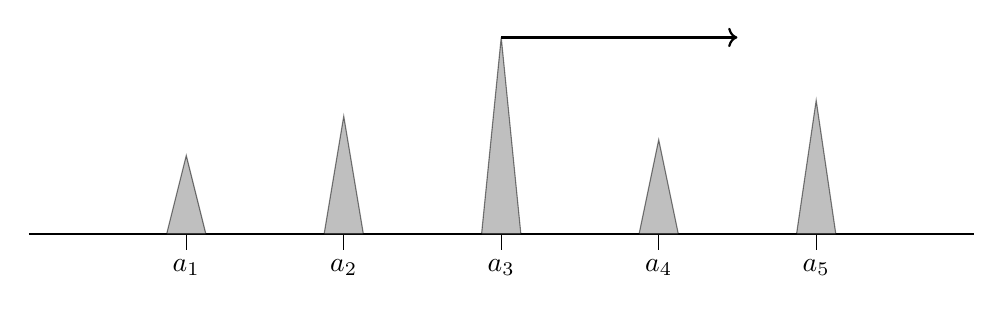
\begin{tikzpicture}

    % Disegna la retta dei numeri
    \draw[thick] (-1, 0) -- (11, 0);

    % Etichette dei punti a1, a2, a3, a4, a5
    \draw (1, 0) -- (1, -0.2) node[below] {$a_1$};
    \draw (3, 0) -- (3, -0.2) node[below] {$a_2$};
    \draw (5, 0) -- (5, -0.2) node[below] {$a_3$};
    \draw (7, 0) -- (7, -0.2) node[below] {$a_4$};
    \draw (9, 0) -- (9, -0.2) node[below] {$a_5$};

    % Disegna i triangoli isosceli (più stretti e di colore grigio)
    \draw[fill=gray, opacity=0.5] (0.75, 0) -- (1, 1) -- (1.25, 0) -- cycle;  % Triangolo in a_1
    \draw[fill=gray, opacity=0.5] (2.75, 0) -- (3, 1.5) -- (3.25, 0) -- cycle;  % Triangolo in a_2
    \draw[fill=gray, opacity=0.5] (4.75, 0) -- (5, 2.5) -- (5.25, 0) -- cycle;  % Triangolo in a_3 (il più alto)
    \draw[fill=gray, opacity=0.5] (6.75, 0) -- (7, 1.2) -- (7.25, 0) -- cycle;  % Triangolo in a_4
    \draw[fill=gray, opacity=0.5] (8.75, 0) -- (9, 1.7) -- (9.25, 0) -- cycle;  % Triangolo in a_5

    % Disegna la semiretta che parte dal vertice del triangolo in a_3 (più lunga)
    \draw[thick, ->] (5, 2.5) -- (8, 2.5);

\end{tikzpicture}
\end{center}
In questo caso, $a_3$ rappresenta un \textit{picco} della successione, perchè nessun valore della successione ha un valore più alto.
\\
Ora, abbiamo due casi possibili:
\begin{itemize}
    \item O ci sono \textbf{infiniti picchi}
    \item O ci sono \textbf{finiti picchi}
\end{itemize}
\newpage
\begin{center}
    \textbf{Picchi infiniti}
    \end{center}
    Sia $n_1 \in \mathbb{N}$ il primo picco.
    \\
    Osservo che, essendo infiniti i picchi, se chiamo $P \subset \mathbb{N}$, allora ho definito l'insieme dei picchi, ossia
    \begin{equation}
        P=\{n \in \mathbb{N} | \,\,\, \mbox{$n$ è picco}\,\,\}
    \end{equation}
    Allora ho che $P-\{n_1\}\neq \varnothing$, perchè se no avremmo un solo picco, ma invece abbiamo ipotizzato che ne abbiamo infiniti.
    \\
    Chiamo allora $n_2$ il primo picco di $P-\{n_1\}$.
    \\
    Osservo che $n_1<n_2$ e che $a_{n_1} \geqslant a_{n_2}$, proprio perchè $a_{n_1}$ è un picco.
    \\
    Osservo ora che $P-\{n_1,n_2\}\neq \varnothing$, perchè abbiamo sembra infiniti picchi.
    \\
    Chiamo $n_3$ il primo picco di $P-\{n_1,n_2\}$ e allora ho che:
    \\
    $n_2<n_3$, mentre $a_{n_2}\geqslant a_{n_3}$, proprio perchè $a_2$ è picco.
    \\
    Itero la costruzione, fino ad osservare che ottengo una successione infinita di valori $n_k \in \mathbb{N}$ tali che $a_{n_k}>a_{n_k+1}$, dunque, in sintesi, ottengo una \textbf{sottosuccessione decrescente} (dunque anche monotona).
\begin{center}
\textbf{Picchi finiti}
\end{center}
Se invece $a_n$ a picchi finiti, il nostro insieme $P$ è \textbf{finito}.
\\
Chiamo $n_1 \in \mathbb{N}$ l'elemento che \textbf{\textit{maggiora strettamente}}(ossia $n_1 \notin P$) l'insieme $P$.
\\
Si osserva che \underline{$n_1$ NON è un picco}, perchè $n_1 \notin P$.
\\
So però che $\exists$ $n_2 >n_1$ tale che $a_{n_2}>a_{n_1}$, altrimenti avrei che $\forall \,\,\, n>n_1$ ci sarebbe $a_{n}<a_{n_1}$, e in quel caso avremmo $n_1$ picco, ma, per come lo abbiamo definito, questo non può succedere.
\\
Osservo dunque che neanche $n_2$ è picco, perchè $n_1$ maggiorava strettamente l'insieme $P$, dunque ogni elemento a lui maggiore non apparterrà a $P$, per cui si ha che $n_2$ non è picco.
\\
Iterando il processo trovo
\begin{equation}
    n_1<n_2<n_3<n_4<n_5... \,\,\, \mbox{con} \,\,\, a_{n_1}<a_{n_2}<a_{n_3}<a_{n_4}<a_{n_5}...
\end{equation}
Ho allora trovato una successione \textbf{monotona crescente}

\begin{center}
   \textbf{\textit{ Definizione di successione di Cauchy}}
\end{center}
Diremo che una successione $a_n$ è \virgolette{di Cauchy} se
\begin{equation}
    \forall \,\,\,\, \varepsilon >0 \,\,\, \exists \,\,\, N>0 \,\,\,\mbox{tale che}\,\,\, \forall n,m>N
\end{equation}
\begin{equation}
    |a_n-a_m|<\varepsilon
\end{equation}
\section{Teorema di caratterizzazione delle successioni convergenti}
\begin{thm}
    Una successione $a_n$ è convergente ($a_n \to a \in \mathbb{R}$) $\Longleftrightarrow$ $a_n$ è di Cauchy
\end{thm}
\begin{proof}
\begin{center}
       ($\Rightarrow$) 
\end{center}
E' noto che $a_n$ converge ad $a$, ossia:
\begin{equation}
    \forall \,\,\, \overline{\varepsilon}>0 \,\,\, \exists N>0 \,\,\, \mbox{tale che, se} n>N
\end{equation}
\begin{equation}
    |a_n-a|<\varepsilon
\end{equation}
Fisso adesso $\varepsilon>0$, ho dunque che $a_n-a_m$, $\forall \,\, n,m \in \mathbb{N}$
\begin{equation}
    |a_n-a_m|\leqslant |a_n-a|+|a-a_m|
\end{equation}
Scelgo allora un $N>0$ tale che, se $K>N$, $|a_k-a|<\frac{\varepsilon}{2}$.
\\
Dunque, se $n,m>N$, segue che $|a_n-a_m|<\frac{\varepsilon}{2}+\frac{\varepsilon}{2}$




    \begin{center}
        ($\Leftarrow$)
    \end{center}
    Se $a_n$ è di Cauchy, voglio dimostrare che $a_n$ è convergente, cioè che $\exists \,\,\, a \in \mathbb{R}$ tale che $a_n \to a$
\begin{enumerate}
    \item $\{a_n\}$ limitata:
    \\
    Fisso $\varepsilon=1$, e so che $\exists \,\,\, N \in \mathbb{N}$ tale che, se $n,m>N$, allora $|a_n-a_m|<1$.
    \\
    In particolare, $\forall \,\,\, n>N$ e $m=N+1$, ossia
    \begin{equation}
        |a_n-a_{N+1}|<1
    \end{equation}
    Dunque
    \begin{equation}
        a_{N+1}-1<a_n<a_{N+1}+1
    \end{equation}
Pongo dunque $c=max\{|1+a_{N+1}|,|a_{N+1}-1|,|a_0|,|a_1|,...,|a_N|\}$
\\
Se $n \in \{0,1,...,N\}$, allora $-c<a_n<c$.
\\
Se invece $n>N$, allora $-c<a_n<c$ 
\item $\exists \,\,\, a_{m_n}$ convergente:
\\
E' il teorema di Bolzano-Weierstrass.
\\
In particolare, diciamo che
\begin{align*} 
a_{m_n} \to a &, a \in \mathbb{R}\\
n \to +\infty 
\end{align*}
\item Dimostriamo che $a$ è proprio il limite di $a_{m_n}$.
\\
Fisso $\varepsilon>0$ e cerco $N>0$ tale che, se $n>N$
\begin{equation}
    |a_n-a|<\varepsilon
\end{equation}
Inoltre, $\forall \,\,\, m_n \in \mathbb{N}$ ho che $|a_n-a|\leqslant|a_n-a_{m_n}|+|a_{m_n}|$
   
\end{enumerate}
\begin{itemize}
    \item Se scelgo $N>0$ tale che $|a_{m_n}-a|<\frac{\varepsilon}{2}$ per $n>N$ (cosa che posso supporre dato che $a_{m_n} \to a$ quando $n \to +\infty$) e $N>0$(lo stesso di prima) tale che $|a_n-a_m|<\frac{\varepsilon}{2}$.
    \\
    Dunque, per $n,m>N$, ho anche $|a_n-a_{m_n}<\frac{\varepsilon}{2}$ (poiché $m_n>n$).
    \\
    Concludo che, per $n>N$, $|a_n-a|<\frac{\varepsilon}{2}+\frac{\varepsilon}{2}$

\end{itemize}
    \end{proof}

\section{Successioni ricorsive}
\begin{center}
    \textbf{\textit{Definizione}}
\end{center}
    Una successione $\{a_n\}$ è definita per ricorrenza se:
    \begin{equation}
\begin{cases}
    a_0= \alpha \in \mathbb{R}\\
    a_{n+1}= f(a_n), & f: \mathbb{R} \to \mathbb{R}
\end{cases}
\end{equation}
\begin{center}
    \textbf{\textit{Esempio}}
\end{center}
    \begin{equation}
      a_n=  \begin{cases}
            a_0=1\\
            a_{n+1}=2a_{n}
        \end{cases}
        b_n=\begin{cases}
            a_0=1\\
            a_{n+1}=(n+1)a_n
        \end{cases}
    \end{equation}
    Allora $a_n=2^n$ e $b_n=n!$
\newpage
\subsection{Algoritmo di Erone}
L'algoritmo di Erone è utile per cercare radici quadrate.
\\
Sia dunque $p \in (0,+\infty)$, vogliamo allora cercare $"\sqrt{p}\,"$, ossia un numero $x \in \mathbb{R^+}$ tale che $x^2=p$.
\\
Con l'algoritmo di Erone ci fermiamo alla dimostrazione del fatto che, quanto meno, questo numero esiste.
\begin{center}
    \textbf{\textit{Idea}}
\end{center}
Immaginiamo un quadrato di area $p$, tale dunque che $l^2=p$.
\\
Considero anche un rettangolo di area $p$ e di lati $\alpha>p$ e $\frac{p}{\alpha} < 1$
\\
Allora si ha:
\\
\\
\begin{tikzpicture}
    % Definisci la distanza tra il quadrato e il rettangolo
    \def\distance{1.5}

    % Disegna il quadrato centrato
    \draw[thick] (-4,-2) rectangle (-0,2);
    
    % Scrivi p al centro del quadrato
    \node at (-2,0) {\( p \)};
    
    % Etichetta il lato sinistro con sqrt{p}
    \node[left] at (-4,0) {\( \sqrt{p} \)};
    
    % Etichetta il lato inferiore con sqrt{p}
    \node[below] at (-2,-2) {\( \sqrt{p} \)};
    
    % Disegna il rettangolo spostato a destra del quadrato
    \draw[thick] (0 + \distance,-2) rectangle (3 + \distance,3);
    
    % Scrivi p al centro del rettangolo
    \node at (1.5 + \distance,0.5) {\( p \)};
    
    % Etichetta il lato sinistro del rettangolo con alpha
    \node[left] at (0 + \distance,0.5) {\( \alpha \)};
    
    % Etichetta il lato inferiore del rettangolo con p/alpha
    \node[below] at (1.5 + \distance,-2) {\( \frac{p}{\alpha} \)};
    
\end{tikzpicture}
\\
Vogliamo ora trasformare il rettangolo nel quadrato che ci siamo immaginati.
\\
Chiameremo allora $a_0=\alpha$ e $a_1=\frac{1}{2}a_0+\frac{1}{2}\frac{p}{a_0}=\frac{1}{2}(a_0+\frac{p}{a_0})$, dunque $a_1$ è il nuovo \underline{lato verticale}.
\\
Dunque il nuovo rettangolo sarà
\\
\\
\begin{tikzpicture}
    % Disegna il rettangolo centrato nel foglio
    \draw[thick] (-1.5,-2) rectangle (1.5,3);
    
    % Scrivi p al centro del rettangolo
    \node at (0,0.5) {\( p \)};
    
    % Etichetta il lato sinistro del rettangolo con a_1
    \node[left] at (-1.5,0.5) {\( a_1 \)};
    
    % Etichetta il lato inferiore del rettangolo con p/a_1
    \node[below] at (0,-2) {\( \frac{p}{a_1} \)};
    
\end{tikzpicture}
\\
Iterando il processo, alla fine si ottiene
\begin{equation}
    \begin{cases}
        a_0=\alpha \\
        a_{n+1}=\frac{1}{2}(a_n+\frac{p}{a_n})
    \end{cases}
\end{equation}
\newpage
\begin{center}
    \textbf{\textit{Fatto}}
\end{center}
Voglio che il rettangolo mantenga sempre la proprietà per cui l'altezza è maggiore della base, ossia che
\begin{equation}
    a_{n+1}^2\geqslant p
\end{equation}
Infatti
\begin{equation}
    a_{n+1}^2=\frac{1}{4}(a_n+\frac{p}{a_n})^2\geqslant p
\end{equation}
si ottiene allora
\begin{equation}
    a_n^4+2a_n^2p+p^2 \geqslant 4pa_n^2
\end{equation}
da cui
\begin{align*}
    a_n^4-2pa_n^2+p^2 \geqslant 0\\
    (a_n^2-p)^2 \geqslant 0
\end{align*}
Ma, essendo dunque un quadrato perfetto, sarà sempre maggiore o uguale a zero, dunque è sempre vero che l'altezza è maggiore della base.
\\
\begin{center}
    \textbf{\textit{Fatto 2}}
\end{center}
$a_n$ è decrescente, vediamo infatti che 
\begin{equation}
    a_{n+1} \leqslant a_n \Longleftrightarrow \frac{1}{2}(a_n+\frac{p}{a_n}) \leqslant a_n \Rightarrow a_n^2 + p \leqslant 2a_n^2 \Longleftrightarrow a_n^2 \geqslant p 
\end{equation}
Cioè, come risultato finale, otteniamo il \textbf{\textit{Fatto 1}}
\\
\\
Inoltre $l \neq 0$, perchè se $a_n \to 0$, anche $a_n^2 \to 0$, ma questo non andrebbe bene, perchè abbiamo detto che $a_n^2 \geqslant p$, dunque, essendo grandezze maggiori di zero, questo vanificherebbe tutto.
\\
\begin{center}
    \textit{Passo allora al limite}
\end{center}
Riscrivendo $\lim_{n \to \infty}a_{n+1}=\lim_{n \to \infty}\frac{1}{2}(a_n+\frac{p}{a_n})$ una volta passati al limite si ottiene:
\begin{equation}
    l=\frac{1}{2}(l+\frac{p}{l})
\end{equation}
Insomma, $l>0$ soddisfa
\begin{equation}
    l=\frac{1}{2}(l+\frac{p}{l}) \Longleftrightarrow 2l^2=l^2+p \Longleftrightarrow l^2=p
\end{equation}
Insomma, $l=\sqrt{p}$
\newpage
\subsection{Successione di Fibonacci (Spiegazione molto poco precisa nella fase finale)}
Abbiamo
\begin{equation}
    \begin{cases}
        F_0=1\\
        F_1=1\\
        F_{n+1}=F_n+F_{n-1}
    \end{cases}
    \end{equation}

    \begin{center}
        \textbf{\textit{Esercizio}}
    \end{center}
Dimostrare che 
\begin{itemize}
    \item $F_n$ cresce
    \item $F_n \to +\infty$
\end{itemize}
Apparte questa breve parentesi, adesso pongo
\begin{equation}
    \varphi_n=\frac{F_{n+1}}{F_n}=\frac{F_n+F_{n-1}}{F_n}=1+\frac{1}{\frac{F_n}{F_{n-1}}}=1+\frac{1}{\varphi_{n-1}}
\end{equation}
Insomma, ho definito una nuova successione \underline{ricorsiva} tale che
\begin{equation}
    \begin{cases}
        \varphi_0=\frac{1}{1}=1\\
        \varphi_{n+1}=1 +\frac{1}{\varphi_n}
    \end{cases}
    \end{equation}

    \begin{center}
        \textbf{\textit{Osservo}}
    \end{center}
\underline{\textbf{\textit{SE}}} $\varphi_n \to \varphi$, con $\varphi \in \mathbb{R}$, allora $\varphi$ soddisfa, passando a limite:
\begin{equation}
    \varphi=1+\frac{1}{\varphi}
\end{equation}
Ossia
\begin{equation}
    \varphi^2=1+\varphi
\end{equation}
Per cui la soluzione sarà $\varphi_{\pm}=\frac{1 \pm \sqrt{5}}{2}$
\begin{center}
    \textbf{\textit{Rapporto aureo}}
\end{center}
Operativamente, se prendo un segmento casuale e lo divido in due parti, una prima parte $a$ e una seconda parte $b$, allora posso imporre
\begin{equation}
    \frac{a}{b}=\frac{a+b}{a}=1+\frac{b}{a}
\end{equation}
Chiamo allora $\varphi=\frac{a}{b}$ come \virgolette{rapporto aureo}
\begin{center}
    \textbf{\textit{Dimostriamo quel \underline{SE} (LEMMA)}}
\end{center}
    Se $a_{n+1}=f(a_n)$, allora
    \begin{enumerate}
        \item $f \nearrow \Rightarrow a_n$ monotona
        \item $f \searrow \Rightarrow p_n=a_{2n}$, $d_n=a_{2n-1}$, e sono entrambe \underline{monotone}
    \end{enumerate}
\begin{proof}
    \begin{center}
        (1. $\Rightarrow$ 2.)
    \end{center}
\begin{equation}
    P_{n+1}=a_{2(n+1)}=a_{2n+1+1}=f(a_{2n+1})=f \circ f(a_{2n})=f \circ f(p_n)
\end{equation}
    Ma abbiamo anche
    \begin{equation}
        f \searrow \Rightarrow f \circ f \nearrow
    \end{equation}
    \begin{center}
        \textbf{\textit{Dimostrazione di $ f \searrow \Rightarrow f \circ f \nearrow$}}
    \end{center}
    Considero $x_1 < x_2$, allora so che, essendo $f$ decrescente, $f(x_1) > f(x_2)$.
    \\
    Consideriamo adesso $f(x_2) < f(x_1)$, per la stessa ragione, avremo che, riapplicando $f$, si ottiene $f(f(x_1) < f(f(x_2))$, cioè ho ottenuto che, $\forall x_2 > x_1$, $f \ f (x_2) > f \ f (x_1)$
    \begin{center}
        \textbf{\textit{Dimostriamo il punto 1.}}
    \end{center}
    Ho due casi
    \begin{center}
        \textbf{\textit{Caso 1}}
    \end{center}
    $a_1 \geqslant a_0$.
    \\
    Allora $a_n$ è \underline{crescente}, infatti chiamo $p_n=a_{n+1} \geqslant a_n$, con $n \in \mathbb{N}$, per cui $P_0$ è dunque \underline{vera}.
    \\
    Se allora $P_n$ è vera, $P_{n+1}$ deve essere vera, infatti, per $P_n$ vera, si ha:
    \begin{align*}
        a_{n+1} \geqslant a_n \\
        f(a_{n+1}) \geqslant f(a_n) \\
        a_{n+2} \geqslant a_{n+1} \Rightarrow P_{n+1} \,\,\,\mbox{vera}
    \end{align*}
    Allora si continua, dunque riprendiamo il fatto che
    \begin{equation}
        \begin{cases}
            \varphi_0=1 \\
            \varphi_{n+1}=1+\frac{1}{\varphi_n}=f(\varphi_n)
        \end{cases}
    \end{equation}
    dove $f(t)=1+\frac{1}{t}$
Osservo allora che
\begin{itemize}
    \item $\varphi_n \geqslant 1$
    \item $f$ è $\searrow$
\end{itemize}
Posso allora dire che $\varphi_{2n} \to l$, con $l \in [1;+\infty) \cup \{+\infty\}$.
\\
Ma $\varphi_{2n+1}=1+\frac{1}{\varphi_{2n}}$, e, passando allora al limite, si ha:
\begin{equation}
    m=1 + \frac{1}{l}
\end{equation}
C'è allora questa relazione tra $l$ ed $m$, per cui, se $l= +\infty$, $m=1$.
\\
Analogamente, $\varphi_{2n+2}=1+\frac{1}{\varphi_{2n+1}}$, per cui, passando al limite, si ottiene
\begin{equation}
    l=1+\frac{1}{m}
\end{equation}
ma questo è un \underline{ASSURDO}, perchè avremmo un'equazione del tipo
\begin{equation}
    +\infty=2
\end{equation}
Inoltre, come abbiamo fatto prima
\begin{equation}
    \begin{cases}
        m=1+\frac{1}{l} \\
        l= 1 +\frac{1}{m}
    \end{cases}
\end{equation}
Ma questo implica
\begin{align*}
       m=1+\frac{1}{1+\frac{1}{m}}=+\frac{m}{m+1}=\frac{m+m+1}{m+1} \\
       m(m+1)=2m+1 \Longrightarrow m^2+m=2m+1\\
       m^2=m+1
\end{align*}
Che, per $m=1+\frac{1}{m}$, è esattamente
\begin{equation}
    m=1+\frac{1}{m}
\end{equation}
\begin{center}
    \textbf{\textit{Stessa cosa per l}}
\end{center}
Infatti, dato $l=m=\varphi$, si ha
\begin{equation*}
    l=m=\varphi=\frac{1 \pm \sqrt{5}}{2} \,\,\,\,\,\,\,\,\,\,\,\,\,\, \mbox{(Scarto $\frac{1 - \sqrt{5}}{2}$ perchè $l,m \geqslant 1$)}
\end{equation*}
Insomma,
\begin{align}
    \varphi_{2n} \to \varphi \\
    \varphi_{2n+1} \to \varphi
\end{align}
Per esercizio si dimostri che \hl{ $\varphi_n \to \varphi$}
\begin{center}
    \textbf{\textit{FINE}}
\end{center}




    
\end{proof}


\subsection{Fatti molto utili (equivalenza asintotica e proprietà base)}
Allora, se ho $a_n \sim b_n$, cioè che
\begin{equation}
    \frac{a_n}{b_n} \to 1
\end{equation}
Allora
\begin{equation}
    \begin{cases}
        a_n \sim \alpha_n \\
        b_n \sim \beta_n
    \end{cases}
    \\
    \longrightarrow a_nb_n \sim \alpha_n\beta_n, \frac{a_n}{b_n} \sim \frac{\alpha_n}{\beta_n}
\end{equation}
NON E' VERO IN GENERALE PERO'.
\\
Perchè, in generale, si osserva che \underline{NON} E' VERO CHE $a_n+b_n \sim \alpha_n+\beta_n$.
\\
Ma se $\frac{b_n}{a_n} \to 0 \,\,\,\,\,\, (|b_n|<< |a_n|)$, allora
\begin{equation}
    a_n+b_n=a_n(1+\frac{b_n}{a_n}) \sim \alpha_n(1+\frac{b_n}{a_n}) \sim \alpha_n \sim \alpha_n+\beta_n
\end{equation}
\begin{center}
    \textbf{\textit{Osservazione}}
\end{center}
Se $a_n \sim \alpha_n \nRightarrow e^{a_n} \texttildelow e^{\alpha_n}$

\newpage
\section{Limiti di Funzioni}
\begin{center}
\textbf{Definizione di limite di funzione}
\end{center}
    \begin{equation}
        f= D \to \mathbb{R}
    \end{equation}
    Con $D \subset \R$ dominio di $f$.
    \subsection{Limite finito al finito}
Sia $x_0 \in Acc(D)$ ($X_0$ punto di accumulazione per $D$), sia $l \in \R$.
\\
Diremo che $f(x)$ tende ad $l$ per $x$ che tende a $x_0$ e scriveremo $\lim_{x \to x_0} f(x) = l$ oppure $\underset{x \to {x_0}}{f(x) \to l}$
\\
Dunque:
\begin{equation}
    \mbox{Se} \,\,\,\, \forall \,\, \varepsilon > 0 \,\,\, \exists \,\,\, \delta > 0 \,\,\,\,\,\, \mbox{tale che} \,\,\,\,\,\, \forall x \in D(f), \,\, x \neq x_0, |x-x_0| < \delta, \,\,\,\,\,\, \mbox{vale che} \,\,\,\, |f(x)-l| < \varepsilon
\end{equation}

    \textbf{\textit{Idea }}
L'idea del concetto di limite è che, scelto un qualsiasi punto nella \virgolette{scatoletta} delle $x$ che abbiamo definito, allora si finisce nella \virgolette{scatoletta} delle $y$.
\\
Si osservi inoltre come trovato un $\delta$, allora ne ho trovati infiniti, perchè posso sempre prenderne uno più piccolo per avere la certezza che tutte le immagini finiscano nella scatoletta delle $y$.
\subsection{Ma perchè abbiamo detto che $x \neq x_0$???}
Allora, il fatto è complicato e semplice allo stesso tempo.
\\
Non si prende $x_0$ per una questione legata al fatto che il limite può avere un determinato valore $l$ anche se magari $f(x_0)=m$, dunque se prendessi anche $x_0$, allora starei dicendo una falsità.
\subsubsection{Esempi e esercizi vari (alla fine è uno)}
\begin{itemize}
    \item Usa la definizione di limite per dimostrare che $\lim_{x \to 0}\frac{1}{x}$ non esiste
\end{itemize}
\newpage
\subsection{Limite infinito al finito}
\begin{equation}
    \lim_{x \to x_0}f(x)=l, \,\,\,\, l=\pm\infty
\end{equation}
\begin{center}
    \textbf{\textit{Caso di $l=+\infty$}}
\end{center}
In questo caso si avrà che $\forall \,\,\, M>0 \,\,\, \exists \,\, \delta $ tale che $\forall \,\,\,\, x \in D(f)$, allora $0<|x-x_0|<\delta$, per cui $f(x)>M$
\\
In questo caso $x=x_0$ sarà denominato \underline{\textbf{Asintoto verticale}} della funzione (al contrario è uguale ma con $f(x)<-M$.
\subsection{Limiti destri e sinistri (hanno senso solo per limiti al finito)}
Diremo che $f(x) \to l$ da sinistra (ma anche da destra, analogamente), quando scriviamo
\begin{equation}
    \lim_{x \to x_0^\pm}f(x)=l \,\,\,\,\, (l \in \tilde{\mathbb{R}})
\end{equation}
Ossia, esplicitando
\begin{equation}
    \forall \,\,\, \varepsilon>0 \,\,\, \exists \,\,\, \delta>0, \,\,\,\, 0<|x-x_0|<\delta, \,\,\, x \in D(f)
\end{equation}
Allora avremo $|f(x)-l|<\varepsilon$,\,\, CON\,\,\, $x < x_0$ (o $x>x_0$ nel caso il limite sia destro)
\begin{lem}
    Sia $x_0 \in \mathbb{R}$, $l \in \tilde{\mathbb{R}}$.
    \\
    Allora
    \begin{align*}
        f(x) \to l \\
      \mbox{per} \,\,\,  x \to x_0
    \end{align*}
    Se e solo se
    \begin{equation}
        \begin{cases}
            f(x) \to l
            \\ x \to x_0^-
        \end{cases}
        \begin{cases}
            f(x) \to l \\
            x \to x_0^+
        \end{cases}
    \end{equation}
\end{lem}
\begin{proof}
\begin{center}
    ($\Longrightarrow$)
\end{center}
    Se vale che
    \begin{equation}
        \forall \,\,\, \varepsilon>0 \,\,\, \exists \,\,\,\ \delta>0, x \in D(f), \,\,\, x \neq x_0, |x-x_0|<\delta 
    \end{equation}
    Da cui $|f(x)-l|<\varepsilon$, allora sicuramente vale che $|f(x)-l|<\varepsilon$ è vera per $x$ tale che $|x-x_0|<\delta$ e $x<x_0$
    [Insomma, se $\forall \,\,\, x \in D(f)-\{x_0\}$ tali che $x \in (x_0-\delta;x_0+\delta)$ vale una proprietà qualsiasi, allora varrà anche per $x \in (x_0-\delta,x_0)$]
    \begin{center}
    ($\Longleftarrow$)
\end{center}
So che $\lim_{x \to x_0^{\pm}}f(x)=l$, dunque si ha che, esplicitando
\begin{equation}
    \forall \,\,\, \varepsilon>0 \,\,\, \exists \,\,\, \delta^- >0 \,\,\, \mbox{tale che} \,\,\, x \in (x_0-\delta;x_0)
\end{equation}
Il che implica che $|f(x)-l|<\varepsilon$, e ho anche
\begin{equation}
    \forall \,\,\, \varepsilon>0 \,\,\, \exists \,\,\, \delta^+ >0 \,\,\, \mbox{tale che} \,\,\, x \in (x_0;x_0+\delta)
\end{equation}
Da cui $|f(x)-l|<\varepsilon$.
\\
Ora, dato $\varepsilon>0$, trovo un $\delta>0$ tale che, se $x \in (x_0-\delta;x_0+\delta)-\{x_0\}$, allora $|f(x)-l|<\varepsilon$.
\\
Prendo allora $\delta=min\{\delta^+;\delta^-\}>0$ e ottengo che
\begin{equation}
    (x_0-\delta;x_0+\delta)-\{x_0\} \subset (x_0-\delta^-;x_0) \cup (x_0;x_0+\delta^+)
\end{equation}
\end{proof}
\subsection{Limite finito all'infinito}
Sia $\lim_{x \to \pm\infty}f(x)=l$, con $l \in \mathbb{R}$.
\\
Questo vuol dire che, al solito
\begin{equation}
    \forall \,\,\, \varepsilon>0 \,\,\, \exists \,\,\, M>0 \,\,\, \mbox{tale che}\,\,\, x \in D(f), \,\,\, x>M, \,\, \mbox{allora} \,\,\, |f(x)-l|<\varepsilon
\end{equation}
\subsection{Limite infinito all'infinito}
Sia $\lim_{x \to \pm\infty}f(x)=\pm\infty$.
\\
Allora si ha che
\begin{equation}
    \forall \,\,\, M>0 \,\,\, \exists \,\,\, N>0 \,\,\, \mbox{tale che, se}\,\,\, x  \lessgt \pmN, \,\,\, \mbox{allora} f(x)> \lessgt \pm M
\end{equation}

\subsection{Definizioni varie}
\begin{definition}
    Se $f(x) \to \pm\infty$ per $x \to x_0$, allora diremo che $f(x)$ ha un asintoto verticale in $x_0$
\end{definition}
\begin{definition}
    Se $f \to \pm\infty$ per $x \to x_0^\pm$, si ha un asintoto verticale destro o sinistro
\end{definition}
\begin{definition}
    Se $f \to l \in \mathbb{R}$ per $x \to \pm\infty$, si ha un \underline{asintoto orizzontale}
\end{definition}
\begin{definition}
    Se $f \to \pm\infty$ per $x \to \pm\infty$, allora $f$ ha un asintoto obliquo se vale che \\$\frac{f(x)}{x} \to m$ e che $f(x)-mx \to q$, con $m,q \in \mathbb{R}$
\end{definition}
\begin{center}
    \textbf{\textit{Ricordiamo che}}
\end{center}
\begin{itemize}
    \item $f$ è monotona se $f(x) \leqslant f(y) \,\,\, \forall x \leqslant y$ (crescente) o $\forall \,\,\, x \geqslant y$ (decrescente)
    \item $
    Inf(f)=Inf(Im(f))=inf\{f(A)\}$
    \\
    (Analogamente $sup(f)=sup\{f(A)\}$
\end{itemize}
\section{Teorema del limite di  funzioni monotone}
Sia $f$ definita $f:(-\infty;x_0) \to \mathbb{R}$, $x_0 \in \mathbb{R}$.
\begin{itemize}
    \item Se $f$ è monotona crescente o decrescente, allora
    \begin{equation}
        \lim_{x\to x_0^-}f(x)=\underset{(-\infty, x_0)   }{sup(f)}    
    \end{equation}
    \item Analogamente, se $f: (x_0;+\infty) \to \mathbb{R}$ è crescente o decrescente, allora
    \begin{equation}
     \lim_{x\to x_0^+}f(x)=\underset{(x_0, +\infty)}{inf(f)} 
        \end{equation}

    \end{itemize}
\begin{proof}
    Pongo $l=\underset{(-\infty,x_0)}{sup(f)} $.
    \\
    Mostriamo il caso $l \in \mathbb{R}$ (tutti gli altri casi sono analoghi).
    \\
    Fissiamo allora un $\varepsilon$ e cerchiamo un $\delta >0$ tale che, se $x \in D(f)$ e $x<x_0$, allora $|x-x_0|<\delta$ (ossia $x-x_0 < \varepsilon$), allora $|f(x)-l|<\varepsilon$, ossia
    \begin{equation}
        l-\varepsilon<f(x)<l+\varepsilon
    \end{equation}
    \begin{itemize}
        \item La disequazione $f(x)<l+\varepsilon$ è ovvia, quindi analizziamo l'altra
        \item Mostriamo che $f(x)>l-\varepsilon$ è vera.
        \\
        Per il teorema di caratterizzazione, $\exists \,\,\, \overline{x} \in (-\infty,x_0)$ tale che $f(\overline{x})>l-\varepsilon$
        \item Ma allora, se pongo $\delta=x_0-\overline{x}>0$ (con $x_0-\overline{x}>0$ perchè $\overline{x}<x_0)$.
        \\
        Dunque $x>\overline{x}$ $\Longleftrightarrow x_0-x<\delta$, allora
        \begin{equation}
            f(x)>f(\overline{x}) \,\,\, \mbox{(Perchè f è crescente)}
        \end{equation}
        Da cui
        \\
        \begin{equation}
            \forall \,\,\, x \in (x_0-\delta,x_0), \,\, f(x)> l- \varepsilon
        \end{equation}
    \end{itemize}
\end{proof}
\section{Definizione di limite per successione}
Sia $x_0 \in \tilde{\mathbb{R}}$.
\\
Diciamo che $\lim_{x \to x_0}f(x)=l$ se:
\\
$\forall$ successione $\{x_n\}$ tale che
\begin{align*}
    x_n \to x_0 \\
    x_n \neq x_0
\end{align*}
Vale allora che $f(x_n) \to l$
\begin{center}
    \textbf{\textit{Osservazione}}
\end{center}
$\{f(x_n)\}$ è una successione che associa ad ogni $n \in \mathbb{N}$ un valore $y_n=f(x_n)$
\begin{center}
    \textbf{\textit{Mostriamo ora che $sin(\frac{1}{x}$) non ha limite}}
\end{center}
\begin{center}
    \textbf{\textit{Semplificazione 1}}
\end{center}
Per semplificarci la vita, dimostrare che $sin(\frac{1}{x})$ non ha limite equivale a dimostrare che non ammette limite destro, per cui, per la definizione di limite, non avrà limite in senso ampio.
\begin{center}
    \textbf{\textit{Si ricordi che}}
\end{center}
Una successione $\{x_n\}$ non ammette limite qualora esistano due sottosuccessioni che presentano limiti pari a valori distinti.
\\
\textbf{Cerco allora} due sotto successioni che chiamerò $x_n$ e $y_n$ tali che 
\begin{align*}
    x_n \to 0 & \,\,\,\,\,\,\,\,\,\, y_n \to 0\\ 
    \sin(\frac{1}{x_n}) \to l & \,\,\,\,\,\,\,\,\,\,\sin(\frac{1}{y_n}) \to m
\end{align*}
Con $l \neq m$
\\
Trovo dunque queste due successioni:
\begin{align}
    x_n=\left(\frac{\pi}{2}+2k\pi\right)^{-1} \to 0 \\
    y_n=\left(-\frac{\pi}{2}+2k\pi\right)^{-1} \to 0
\end{align}
Tali per cui
\begin{align}
    \sin(\frac{1}{x_n})=1 \\
    \sin(\frac{1}{y_n})=-1
\end{align}
Ho dunque trovato due sottosuccessioni tali per cui la funzione $\sin(\frac{1}{x})$ non ammette limite
\newpage
\section{Teorema del collegamento}
Il teorema del collegamento ci permette di \virgolette{convertire} tutto ciò che è stato dimostrato per i limiti di successione, rendendolo di fatto valido per i limiti di funzione
\begin{center}
    \textbf{\textit{Teorema del collegamento}}
\end{center}
Il teorema del collegamento relaziona con un SE E SOLO SE (\textbf{relazione di equivalenza}) le seguenti affermazioni:
\begin{enumerate}
    \item $\lim_{x \to \overline{x}}f(x)=l$, con $\overline{x} \in Acc(f)$, $l \in \tilde{\mathbb{R}}$ oppure $\overline{x} \in \{\pm\infty\}$
    \item $\forall$ successione $\{x_n\}$ tale che $x_n \to \overline{x}$, con $x_n \neq \overline{x}$ (definitivamente) vale che $f(x_n) \to l$

\end{enumerate}
Colleghiamo di fatto le successioni ai limiti
\begin{proof}
    \begin{center}
        (2. $\Longrightarrow$ 1.) (RAA)
    \end{center}
    Per dimostrare questa parte del teorema l'idea è quella di supporre che non esista il limite del punto 1, e ragionare per assurdo sulle implicazioni.\\ Per ASSURDO
    $\exists \,\,\, \overline{\varepsilon}>0$ tale che $\forall \,\,\, \delta>0 \,\,\,\exists  x_{\delta} $, con $x_\delta \neq \overline{x}$, per cui $|x_\delta-\overline{x}|<\delta$, ma $|f(x_\delta)-l| \geqslant \varepsilon$.
    \begin{itemize}
        \item Fisso $\delta_1=1$, allora trovo $x_1 \in Acc(D(f))-\{\overline{x}\}$, per cui $|x-\overline{x}|<1$, ma $|f(x_1)-l|\geqslant \varepsilon$
        \item Fisso $\delta_2=\frac{1}{2}$, per cui
        \begin{equation}
            \begin{cases}
                |x_2-\overline{x}|<\frac{1}{2} \\
                |f(x_2)-l| \geqslant \overline{\varepsilon}
            \end{cases}
        \end{equation}
    \end{itemize}
Iterando questo processo si ottiene, per $n \in \mathbb{N}$, $\delta_n=\frac{1}{n}$, per cui $\exists \,\,\, x_n \in A$ per cui vale
\begin{equation}
    \begin{cases}
        |x_n-\overline{x}|<\frac{1}{n} \\
        |f(x_n)-l| \geqslant \overline{\varepsilon}
    \end{cases}
\end{equation}
    Per come la abbiamo definita, abbiamo allora trovato una successione che soddisfa queste ultime due equazioni contemporaneamente, per l'n-esimo termino vale sempre la disuguaglianza $|x_n-\overline{x}|<\frac{1}{n}$.
    Ora, sappiamo che:
    \begin{itemize}
        \item $x_n \to \overline{x}$, infatti $0<|x_n-\overline{x}|<\frac{1}{n}$, per cui $|x_n-\overline{x}| \to 0$.
        \\
        Inoltre, per il lemma tale che $|a_n|\to 0$, allora $a_n \to 0$, si ha che $x_n-\overline{x} \to 0$, e infine, per l'algebra dei limiti, si ottiene che
        \begin{equation}
            x_n \to x
        \end{equation}
        Ma allora si ha che $f(x_n) \to l$, e dunque che $|f(x_n)-l|\to 0$.
        \\
        Ma $|f(x_)-l| \geqslant \overline{\varepsilon}>0$, e, per il teorema del confronto si giunge a
        \begin{align}
            \lim_{n \to +\infty}y_n \geqslant \overline{\varepsilon} \\
            0 \geqslant \varepsilon
        \end{align}
        Ma questo è un ASSURDO!
    \end{itemize}
    \begin{center}
        (1. $\Longrightarrow$ 2.)
    \end{center}
    Voglio dimostrare che, data la successione $\{x_n\} \subset D(f)-\{\overline{x}\}$, tale che $x_n \to \overline{x}$.
    \\
    Allora $y_n=f(x_n) \to l$.
    \\
    Questo vuol dire che, dato $\varepsilon>0$, \underline{dobbiamo trovare un $N>0$} tale che, se $n>N$, allora $|f(x_n)-l|<\varepsilon$.
    \\
    \begin{itemize}
        \item Sappiamo che, dato $\varepsilon$ fissato, sicuramente, per la definizione di limite, $\exists \overline{\delta}>0$ tale che, se $0<|x-\overline{x}|<\overline{\delta}$, allora $|f(x)-l|<\varepsilon$
        \item So anche che, fissato $\overline{\delta}>0$, allora $\exists \,\,\, N>0$ tale che, se $n>N$, allora $|x_n-\overline{x}|<\delta$.
        \\
        Dunque, dato $\varepsilon > 0$, $\exists \,\,\, \overline{\delta}_\varepsilon > 0$ tale che $\exists \,\,\, N>0$ tale che, se $n>N$, $|x_n-\overline{x}| < \overline{\delta}_\varepsilon\,\,\,\,\,\,\, \Longrightarrow \,\,\,\,\,\, |f(x_n)-l|<\varepsilon$, dove nell'ultimo passaggio ho usato il primo punto (Sappiamo che...) con $x_n$ al posto di $x$
    \end{itemize}
\end{proof}

\subsection{Corollari del teorema del collegamento}
\subsubsection{Algebra dei limiti}
Siano $f,g$ funzioni reali.
\\
Prendo $\overline{x_0} \in Acc(f) \cap Acc(g)$, allora:
\begin{itemize}
    \item Se $f(x) \to l$ per $x \to x_0$
    \item Se $g(x) \to m$ per $x \to \overline{x_0}$
\end{itemize}
Allora $f (+,-,\div,\times) g) \to l (+,-,\div,\times) m$, per $x \to x_0$.\\
In poche parole, operazioni tra limiti danno somma, sottrazione, moltiplicazione o divisione dei risultati dei limiti.\\
\begin{center}
    \textbf{\textit{Ad esempio la somma}}
\end{center}
\begin{proof}
Per la somma infatti, possiamo dimostrare che
\begin{equation}
    f(x)+g(x) \to l+m
\end{equation}
Sia $x_n \to \overline{x_0}$, con $x_n \neq x_0$ definitivamente.
\\
Allora
\begin{equation}
    f(x_n)+g(x_n) \to l+m
\end{equation}
Poiché $f(x_n) \to l$ e $g(x_m) \to m$, per il \underline{teorema del collegamento} e per l'algebra dei limiti delle successioni.
\\
Infine, per il teorema del collegamento (al contrario però), si ottiene 
\begin{equation}
    f+g \to l+m
\end{equation}
\end{proof}
\subsection{Teorema dei carabinieri}
Sia $\overline{x} \in Acc(f) \cap Acc(g) \cap Acc(h)$, dove $f,g,h$ sono funzioni reali.
\\
Allora, se $f \leqslant g \leqslant h$ e $\lim_{x \to \overline{x}}f(x)=l=\lim_{x \to \overline{x}}$, si ha che $g(x) \to l$ per $x \to x_0$
\begin{proof}
    Fisso $x_n \to \overline{x}$, per il \underline{teorema del collegamento} si ha che $f(x_n) \to l$ e $h(x_n) \to l$.
    \\
    Continua però a valere la disequazione $f(x_n) \leqslant g(x_n) \leqslant h(x_n)$, allora, per il teorema dei carabinieri delle successioni, si avrà che
    \begin{equation}
        f(x_n) \to l \leqslant g(x_n) \leqslant h(x_n) \to l
    \end{equation}
    Per il \underline{teorema dei carabinieri delle successioni} si ha che $g(x_n) \to l$ e, valendo $\forall \,\,\, \{x_n\}$, per il teorema del collegamento si ottiene che
    \begin{align*}
        g(x) \to l \\
        x_n \to \overline{x}
    \end{align*}
\end{proof}
\subsection{Corollario teorema dei carabinieri}
Se $f(x) \to +\infty$ per $x \to \overline{x}$ e $f \leqslant g$, allora
\begin{align*}
    g(x) \to +\infty \\
    x_0 \to \overline{x}
\end{align*}
\begin{proof}
   Sia $x_n \to x_0$, allora, per il teorema del collegamento, $f(x_n) \to +\infty$.
   \\
   Per il teorema dei carabinieri per le successioni, vale che $g(x_n) \to +\infty$, dunque, per il teorema del collegamento (inverso) vale $\lim_{x \to x_0}g(x)=+\infty$
\end{proof}
\newpage
\subsection{Prodotto funzione limitata per funzione infinitesima}
Se $f(x) \to 0$ per $x \to \overline{x}$.
\\
Se $g(x)$ è una funzione limitata, cioè $\exists \,\,\, c$ tale che $|g(x)|\leqslant c \,\,\, \forall x \in D(g)$.
\\
Allora $f \cdot g \to 0$ per $x \to \overline{x}$
\begin{proof}
    Se $x_n \to \overline{x}$, allora $f(x_n) \to 0$, e $g(x_n)$ è una successione limitata.
    \\
    Allora si ha che:
    \begin{align}
        f(x_n)g(x_n) \to 0 \\
        x \to \overline{x}
    \end{align}
    Come già dimostrato nelle successioni.
    \\
    Allora, per \underline{il teorema del collegamento}, $f(x)g(x) \to 0$
\end{proof}
\subsection{Teorema di confronto (permanenza del segno)}
Sia $\overline{x} \in Acc(f)$, sia $l \in \mathbb{R}$.
\begin{enumerate}
    \item Se $f(x) \to l$ per $x \to \overline{x}$ e $l>0$, allora esiste un intorno di $\overline{x}$, ossia ($I-\{\overline{x}\}$), tale che $\forall x \in I$, $f(x)>0$.
    \\
    Ossia $\exists \varepsilon>0$ tale che se $x \in (\overline{x}-\varepsilon, \overline{x}+\varepsilon)-\{\overline{x}\}$, allora $f(x) > 0$
    \item Se $f(x)>0 \,\,\, \forall \,\,\, x$ in un intorno di $\overline{x}$, con $x \neq \overline{x}$, allora si ha, se 
    \begin{equation}
        f(x) \to l
    \end{equation}
    Che
    \begin{equation}
        l \geqslant 0
    \end{equation}
\end{enumerate}
\begin{proof}[]
\begin{center}
    \textbf{\textit{Dimostrazione di (2)}}
\end{center}
Sia $f(x)\to l$
    \\
    Sia $x_n \to \overline{x}$, allora $f(x_n)>0$ (definitivamente).
    \\
    Questo perchè $\exists \,\,\, \varepsilon>0$ tale che, se $0< |x-\overline{x}|<\varepsilon$, allora $f(x)>0$, e inoltre
    \begin{equation}
        |x_n-\overline{x}|<\varepsilon \,\,\, \mbox{definitivamente} \Longrightarrow f(x_n)>0 \,\,\,\mbox{definitivamente}
    \end{equation}
    \\
    Inoltre, $f(x_n) \to l$ per il teorema del collegamento, e, per il teorema di confronto delle successioni allora, è noto che $l \geqslant 0$.
    \begin{center}
        \textbf{\textit{Dimostrazione di 1.}}
    \end{center}
    Fissiamo un $\overline{\varepsilon}=\frac{l}{2}>0$, allora è noto che
    \begin{equation} \label{eq1}
        |f(x)-l|<\frac{l}{2} \,\,\, \mbox{per} \,\,\, x \in I(\overline{x})-\{\overline{x}\}.
    \end{equation}
    Ossia, se $|x-\overline{x}|<\varepsilon$, con $x \neq \overline{x}$, $\forall \,\,\, \varepsilon>0$ (bisogna precisare che questo $\varepsilon$ è il $\delta>0$ della definizione, chiaro.)
    \\
    Ora, l'equazione \ref{eq1} implica che
    \begin{align*}
        \frac{l}{2}<f(x)<\frac{3}{2}l \\
        f(x)>\frac{l}{2} \,\,\, \forall \,\,\, x \in (\overline{x}-\varepsilon;\overline{x}+\varepsilon)-\{\overline{x}\}
    \end{align*}
\end{proof}

\subsection{Teorema del cambio di variabile}
Si ha che $\lim_{x \to x_0}f(g(x))=\lim_{y \to y_0}f(y)$ \underline{SE} \begin{itemize}
    \item $x_0 \in Acc(g)$
    \item $y_0 \in Acc(f)$
    \item $g(x) \to y_0$
    \item $g(x) \neq y_0$ in un intorno di $x_0$
\end{itemize}
\begin{center}
    \textbf{\textit{Dimostrazione}}
\end{center}

    \item Suppongo sia finito il $\lim_{y \to y_0}f(y)=l$.
    \\
    \item Fisso$\varepsilon>0$ e CERCO se $\exists \,\,\, \overline{\delta} >0$ tale che, se $|x-x_0|<\overline{\delta}$
    \begin{equation}
        |f(g(x))-l|<\varepsilon
    \end{equation}
 \begin{enumerate}
\item ($\underset{x \to x_0}{g(x)-y_0}$) $\forall \varepsilon > 0\ \exists \delta_1 > 0$ tale che $|x - x_0| < \delta_1 \Rightarrow |g(x) - y_0| < \varepsilon$
\item ($\underset{y \to y_0}{f(y) \to \ell}$)$\forall \overline{\varepsilon} > 0\ \exists \delta_2 > 0$ tale che $|y - y_0| < \delta_2 \Rightarrow |f(y) - \ell| < \overline{\varepsilon}$
\end{enumerate}

Scegliamo $\overline{\varepsilon} = \delta_2$. Allora:
\[
|x - x_0| < \delta_1 \Rightarrow |g(x) - y_0| < \delta_2 \Rightarrow |f(g(x)) - \ell| < \varepsilon
\]


\end{itemize}
Se $g(x) \neq y_0$ in un intorno bucato di $x_0$, la dimostrazione è analoga considerando:
\[
x \in (x_0 - \delta, x_0 + \delta) \setminus \{x_0\}
\]

\subsection*{Osservazione finale}
Scegliendo $\delta = \min\{\delta_1, \delta_2\}$ si ottiene la convergenza desiderata.
    \\
   \underline{ (Inoltre, se $\tilde{\delta}(\varepsilon)$ è sufficientemente piccolo, allora $g(x) \neq y_0$.)}
   \\
   Quando diciamo \underline{sufficientemente piccolo}, intendiamo dire che: per ipotesi sappiamo che $g(x) \neq y_0$ in un intorno di $x_0$, questo vuol dire che
   \begin{equation}
       \exists \,\,\, \gamma > 0 \,\,\,\,\, \mbox{tale che} \,\,\,\,\,\ \forall x \in (x_0-\gamma, x_0+\gamma) \,\,\,\,\,\,\, \mbox{per cui} \,\,\,\,\, g(x) \neq y_0
   \end{equation}
   Dunque scelgo $\tilde{\tilde{\delta}}=min(\tilde{\delta},\gamma)$, così sono sicuro che all'interno dell'intorno vale la mia ipotesi e $g(x) \neq y_0 \forall x$ appartenente all'intorno scelto.
   Per ipotesi:

\newpage
\subsection{Funzioni continue e discontinue}
\subsubsection{Definizione di funzione continua in un punto}
Sia $f: D \subset \mathbb{R} \to \mathbb{R}$.
\\
Sia $x_0 \in D$. 
\\
Diremo allora che $f$ è continua \underline{in $x_0$} se \begin{itemize}
    \item $\lim_{x \to x_0}f(x)=f(x_0)$, oppure
    \item Se, $\forall \,\,\, \varepsilon>0$ $\exists\,\,\, \delta >0$ tale che, se $|x-x_0|<\delta$, allora $|f(x)-f(x_0)|<\varepsilon$.
    \\
    Diremo inoltre che $f$ è continua nel suo dominio $D$ se è continua $\forall \,\,\, x_0 \in D$
\end{itemize}
\subsubsection{Discontinuità di una funzione}
Una funzione \underline{è discontinua se non è continua}
\\
\begin{center}
    \textbf{\textit{Discontinuità di $I$ specie}}
\end{center}
Si dice che $f$ ha una discontinuità di $I$ specie in $x_0$ se
\begin{equation}
    \lim_{x \to x_0^-}f(x)=l \neq m = \lim_{x\to x_0^+}f(x) \in \mathbb{R}
\end{equation}

\begin{center}
    \textbf{\textit{Discontinuità eliminabile}}
\end{center}
Si dice che $f$ ha una discontinuità eliminabile se:
\begin{equation}
    \lim_{x \to x_0^{\pm}}f(x)=l \in \mathbb{R}
\end{equation}
O, equivalentemente, se 
\begin{equation}
    \exists \,\,\, \lim_{x \to x_0^{\pm}}f(x)=l
\end{equation}
MA è noto che $l \neq f(x_0)$
\begin{center}
    \textbf{\textit{Discontinuità di $II$ specie}}
\end{center}
Si dice che $f$ ha una discontinuità di $II$ specie se non ha una discontinuità di $I$ specie
\subsubsection{Esercizio/Teorema non facile}
Se $f(D(f)=\mathbb{R})$ è MONOTONA, allora $f$ ha, al più, una \underline{quantità numerabile} di discontinuità.
\subsubsection{Definizione dell'insieme delle funzioni continue}
Sia $D \subset \mathbb{R}$.
\\
Poniamo $C^0(D)=\{f: D \to \mathbb{R} | f \,\,\, \mbox{è continua in} \,\,\, D=D(f)\}$
\subsection{Operazioni tra funzioni continue}
La domanda fondamentale a cui risponderemo adesso è:
\begin{center}
    \textbf{\textit{Ma come faccio a dire se una funzione $f$ è continua??}}
\end{center}
Siano $f,g : D \to \mathbb{R}$, e sia $x_0 \in Acc(D)$.
\\
Se $f$ e $g$ sono continue in $x_0 \in D$ allora $h=f (+-\times\div)g$ sono continue in $x_0$.
\\
Insomma, qualsiasi operazione faccio tra funzioni continue, la funzione risultante sarà una funzione continua.
\begin{center}
    \textbf{\textit{Dimostrazione}}
\end{center}
Se $f$ e $g$ sono continue in $x_0$, allora:
\begin{align}
    \lim_{x \to x_0}f(x)= f(x_0) \\
    \lim_{x \to x_0}g(x)=g(x_0)
\end{align}
Considero adesso una successione $x_n \to x_0$, con $x_n \in D(f),D(g)$.
\\
Per il teorema del collegamento vale che
\begin{align}
    f(x_n) \to f(x_0) \\
    g(x_n) \to g(x_0)
\end{align}
Per l'algebra dei limiti di successione valgono tutte le regole, per cui $\lim_{x \to x_0} h(x_n) = \lim_{x \to x_0} f(x_n) (+- \times \div) g(x_n)= f(x_0) (+-\times \div) g(x_0)$, per il teorema del collegamento $\lim_{x \to x_0}h(x) \to \lim_{x \to x_0} f(x)(+-\times \div)g(x)= f(x_0) (+- \times \div) g(x_0) = h(x_0)$, dunque $h$ risulta sempre continua.

\subsection{Composizione di funzioni continue è continua}
Sia $x_0 \in Acc(f) \cap Acc(g) \cap Acc(h)$.
\\
Siano $f$ e $g$ funzioni continue. Allora $h= f\circ g$ è una funzione continua.
\begin{center}
    \textbf{\textit{Dimostrazione}}
\end{center}
Sappiamo che:
\begin{align}
    \forall \varepsilon \,\, \exists \,\, \delta' > 0 \,\,\,\, \mbox{t.c.}\,\,\,\,, |x-x_0| < \delta', \,\,\,\,\,\, |g(x)-g(x_0)| < \varepsilon
\end{align}
Dunque è noto che, con un cambio di variabile, $g(x)=y$ e $g(x_0)=y_0$
\begin{equation}
    \forall \varepsilon \,\, \exists \,\, \delta'' > 0 \,\,\,\, \mbox{t.c.}\,\,\,\,, |y-y_0| < \delta'', \,\,\,\,\,\, |f(y)-f(y_0)| < \varepsilon
\end{equation}
In questa maniera ho dimostrato che, per $\delta=min\{\delta',\delta''\}$ si ha che
\begin{equation}
    |f(g(x))-f(g(x_0))|< \varepsilon
\end{equation}
cioè proprio che $\lim_{x \to x_0}h(x)=\lim_{x \to x_0} f(g(x))= f(g(x_0))=h(x_0)$
\subsection{Continuità delle funzioni basilari}
$e^x,\ln{x},x^p,\sin{x},\cos{x},\tan{x},\cosh{x},\sinh{x}$ sono tutte funzioni continue
\begin{proof}
    \begin{itemize}
        \item \begin{center}
            $e^x$ e $\ln{x}$
        \end{center}
        Il processo logico è semplice, partendo da una successione $x_n \to x$, si avrà $e^{x_n}\to e^x$, che implica $\lim_{y \to x}e^y=e^x$(Per il teorema del collegamento)
    \end{itemize}
    \begin{center}
        $x^p$
    \end{center}
    Se riscriviamo $x^p$ come $x^p=e^{p\ln{x}}$ sappiamo che è continua, perchè $\ln{x}$ è continua, dunque la composizione di continue è continua
    \begin{center}
        $\cosh{x}=\frac{e^x-e^{-x}}{2}$ è continua perchè composizione di funzioni continue
    \end{center}
    \begin{center}
       seno e coseno:
    \end{center}
    \begin{itemize}
        \item La funzione seno è continua in $x_0=0$, infatti sia:
        \begin{equation}
            0 \leqslant x \leqslant \frac{\pi}{2}
        \end{equation}
        Applicando la funzione $\sin$ a tutti i membri si ottiene:
        \begin{equation}
            0 \leqslant \sin{(x)} \leqslant x \to 0
        \end{equation}
        Per il teorema dei carabinieri allora $\sin{(x)} \to 0$, inoltre, per simmetria, essendo $\sin{(-x)}=-\sin{(x)}$, si ha che $\lim_{x \to 0^-}\sin{(-x)}=0$
        \item La funzione $\cos$ è continua in 0, perchè possiamo scriverla come
        \begin{equation}
            \cos{x}=\sqrt{1-\sin^2{(x)}}
        \end{equation}
        \item $\cos{(x)} \in C^0(\mathbb{R})$, perchè se prendo una generica $y=x+h$, da cui $\cos{(x+h)}=\cos{(x)}\cos{(h)}-\sin{(x)}\sin{(h)}$.
        \\
        Se $y \to x$, allora $h \to 0$, e dunque $\cos{(y)}=\cos{(x+h)}=\cos{(x)}\cos{(h)}-\sin{(x)}\sin{(h)}$, passando al limite dunque:
        \begin{equation}
            =\cos{(x)}
        \end{equation}
        \item $\sin{(x)} \in C^0(\mathbb{R}$.
        \\
        Questo perchè $\sin{(x)}=\cos{x-\frac{\pi}{2}}$, che dunque $\in C^0(\mathbb{R})$
    \end{itemize}
\end{proof}
\section{Teoremi sulle funzioni continue}
\subsection{Teorema di permanenza del segno}
Sia $f: I \to \mathbb{R}$, con $I$ intervallo.
\\
$x_0 \in I$ .
\\
Se:
\begin{enumerate}
    \item $f \in C^0(I)$
    \item $f(x_0)>0$
\end{enumerate}
Allora $\exists$ un intorno di $x_0$ tale che $f(x)>0$ in tale intorno.
\begin{proof}
    E' noto che $\lim_{x \to x_0}f(x)=f(x_0)>0$, dunque, per il teorema del confronto tra limiti, allora esiste un intorno di $x_0$, $J$, tale che $f(x)$ è positiva in $J - \{x_0\}$.
    \\
    Ciò implica che $f(x)>0 \,\,\,\forall \,\,\, x \in J$, dunque che $f(x_0)>0$
\end{proof}
\subsection{Teorema degli zeri}
Siano $a<b$, con $a,b \in \mathbb{R}$, e sia $f \in C^0([a,b])$.
\\
Supponiamo che $f(a)f(b) \leqslant0$.
\\
Allora $\exists \,\,\, c \in [a,b]$ tale che $f(c)=0$
\begin{proof}
    Wlog (Without Loss Of Generality), possiamo supporre che
    \begin{equation}
        f(a)<0 \,\,\,\,\,\,\,\,\,\,\,\,\, f(b)>0
    \end{equation}
    Controllo poi a metà dell'intervallo il valore della funzione, buttando via la metà che non mi interessa, fino ad arrivare allo 0 che cerchiamo.
    \begin{itemize}
        \item Sia $\alpha$ il punto medio di $[a,b]$, ossia $\alpha=\frac{a+b}{2}$.
        \begin{center}
            \textbf{\textit{Caso 1}}
        \end{center}
        $f(\alpha)=0$, la dimostrazione finisce
        \begin{center}
            \textbf{\textit{Caso 2}}
        \end{center}
        $f(\alpha)>0$, pongo allora $a_1=a$ e $b_1=\alpha$
        \begin{center}
            \textbf{\textit{Caso 3}}
        \end{center}
        $f(\alpha)<0$, pongo allora $a_1=\alpha$ e $b_1=b$
    \end{itemize}
   Richiamo $\alpha$ il punto medio di $a_1$ e $b_1$, ossia $\alpha = \frac{a_1+b_1}{2}$ e ripeto i tre casi:
\begin{center}
    \textbf{\textit{Caso 1}}
\end{center}
$f(\alpha)=0$, ho finito, $c=\alpha$
\begin{center}
    \textbf{\textit{Caso 2}}
\end{center}
$f(\alpha)>0$, allora $a_{2}=a_1$ e $b_{2}=\alpha$
\begin{center}
\begin{center}
    \textbf{\textit{Caso 3}}
\end{center}
\begin{center}
    $f(\alpha)<0$, allora $a_{2}=\alpha$ e $b_{2}=b_1$
    \end{center}
\end{center}
Adesso iteriamo e, se ho costruito $a_n$ e $b_n$ iterando, allora
\begin{equation}
    \alpha = \frac{a_n+b_n}{2}
\end{equation}
Ora, rifacciamo i casi:
\begin{center}
    \textbf{\textit{Caso 1}}
\end{center}
$f(\alpha) = 0$, siamo apposto come al solito
\begin{center}
    \textbf{\textit{Caso 2}}
\end{center}
$f(\alpha) > 0$, allora $b_{n+1}=\alpha$ e $a_{n+1}=a_n$
\begin{center}
    \textbf{\textit{Caso 3}}
\end{center}
$f(\alpha) < 0$, allora $a_{n+1}=\alpha$ e $b_{n+1}=b_n$
\begin{center}
    \textbf{\textit{Osservazioni generali}}
\end{center}
Ora, osserviamo che $a_{n+1} \in [a_n, \alpha]$ e dunque che $a_{n+1} \geqslant a_n$.
\\
Inoltre consideriamo il fatto che $\alpha = \frac{a_n+b_n}{2} \geqslant \frac{a_n+a_n}{2}=a_n$, per cui $a_n$ è crescente.
\\
Analogamente, $b_n$ è decrescente
\\
Inoltre vale che 
\begin{align}
    b \geqslant a_n \geqslant a \,\,\,\,\, \forall n \in \N \\
    a \leqslant b_n \leqslant b \,\,\,\,\, \forall n \in \N 
\end{align}
Per il \underline{teorema delle successioni monotone} si ha che
\begin{equation}
    a_n \to A \,\,\,\,\,\,\,\,\,\,\,\,\,\, b_n\to B
\end{equation}
Inoltre, per il teorema di confronto, si ha che $A,B \in \mathbb{R}$, infatti $A,B \in [a,b]$
\\
Infine sappiamo che 
\begin{align}
    a_n \geqslant a \\
    \lim_{n \to +\infty }a_n \geqslant \lim_{n \to +\infty} a \\
    A \geqslant a
\end{align}
\begin{center}
    \textbf{\textit{Fatto 1}}
\end{center}
$A=B$, poichè si può vedere che $b_1-a_1=b-\frac{a+b}{2}=\frac{b}{2}-\frac{a}{2}$, cioè l'intervallo a metà.
\\
Analogamente, si ha che, \underline{PER INDUZIONE}
\begin{equation}
    b_{n+1}-a_{n+1}=\frac{b_n-a_n}{2}=\frac{b_{n-1}-a_{n-1}}{2^2}=...=\frac{b-a}{2^n}
\end{equation}
Dunque $A-B=\lim_{n\to +\infty}a_n-\lim_{n\to +\infty}b_n=\lim_{n\to +\infty}\frac{1}{2^n}(b-a)=0$, cioè
\begin{equation}
    A=B=\xi
\end{equation}
\begin{center}
    \textbf{\textit{Fatto 2}}
\end{center}
Sia $f(a_n) \leqslant 0$ e $f(b_n) \geqslant 0$.
\\
Questo vuol dire che $f(a_n)f(b_n) \leqslant 0$.
\\
Infine però so che \begin{equation}
    f(a_n) \to f(\xi) \,\,\,\,\,\ \mbox{e}\,\,\,\,\,\,\,\,\,\, f(b_n) \to f(\xi)
\end{equation}
Poichè $f$ è continua per ipotesi.
\\
Ma allora ho concluso, perchè ciò vuol dire che
\begin{equation}
    f(\xi)f(\xi) \leqslant 0 \Longrightarrow f(\xi) = 0
\end{equation}
Pongo $\xi=c$ e ho finito.
\end{proof}
\subsection{Teorema di esistenza della radice n-esima}
Fisso un $y>0$ e un $n \in \mathbb{N}$, con $n \geqslant 2$.
\\
Allora $\exists \,\,\, x \in \mathbb{R}$ soluzione dell'equazione $x^n=y$.
\\
\begin{proof}
\begin{center}
    \textbf{\textit{Caso $y>1$}}
    \end{center}
    Osserviamo che $f(0)=-y <0$
    \\
    Inoltre $f(y)=y^n-y=y(y^{n-1}-1)$.
    \\
    Infine $f \in C^0([0,y])$. Allora, per il teorema degli zeri, esiste $\overline{x}$ tale che $f\overline{x})=0$ ($\overline{x}=y$)
\end{proof}
\subsection{Teorema di Weierstrass}
\subsubsection{Lemma propedeutico}
Sia $f:D \to \mathbb{R}$ una funzione.
\\
$Im(f) \subset \mathbb{R}$ allora ammetterà $sup$ e $inf$, ossia:
\begin{itemize}
    \item $\exists x_n \in D$ tale che $f(x_n) \to sup(f)$ in $D$ ($\{x_n\} \subset D$)
    \item $\exists y_n \in D$ tale che $f(y_n) \to inf(f)$ in $D$ ($\{y_n\} \subset D$).
    \\
\end{itemize}
    In altre parole, $sup$ e $inf$ sono sempre raggiunti da almeno una successione.
\begin{center}
    \textbf{\textit{Dimostrazione}}
\end{center}
Chiamo $\alpha=supD(f)$
\begin{center}
    \textbf{\textit{Caso 1}}
\end{center}
$\alpha \in \mathbb{R}$, so allora che:
\\
$\forall \,\,\, x \in D$ si ha che $f(x) \leqslant \alpha$, inoltre $\forall \,\,\, \varepsilon>0 \,\,\, \exists \,\,\, x \in D$ tale che $f(x) > \alpha - \varepsilon$.
\\
Se inoltre pongo $\varepsilon_n=\frac{1}{n}>0$, troverò una $x_n$ tale che $f(x_n)>\alpha-\frac{1}{n}$.
\\
Questo implica che $\alpha- \frac{1}{n}<f(x_n)<\alpha$.
\\
Per i carabinieri allora, $\lim_{n \to +\infty }f(x_n)= \alpha$.
\begin{center}
    \textbf{\textit{Caso 2}}
\end{center}
Se $\alpha=+\infty$, allora $Im(f)$ non è limitato.
\\
Cioè, $\forall \,\,\, n \in \mathbb{N}$, $\exists \,\,\, x_n$ tale che $f(x_n)>n$.
\\
(Se non fosse così, $\exists n \in \mathbb{N}$ tale che, $\forall \,\,\, x \in D$, $f(x) \leqslant n$, $\forall x \in D$)
\\
Allora ho che $f(x_n) \to +\infty=sup(f)$ in $D$
\subsection{Teorema di Weierstrass}
Sia $f: [a,b]=D(f) \to \mathbb{R}$ una funzione continua ($\in C^0[a,b])$.
\\
Allora $f$ ammette \underline{massimo} e \underline{minimo}.
\begin{proof}
    \begin{center}
        \textbf{\textit{Mostriamo che esiste un massimo}}
    \end{center}
    Mostrare che esiste un massimo equivale a mostrare che $\exists \,\,\, x \in [a,b]$ tale che $f(x)=sup(f)$ in $[a,b]$.
    \\
    \begin{itemize}
        \item Sia $\{x_n\} \in [a,b]$ una successione tale che $f(x_n) \to sup(f)$.
        \\
        Tale successione esiste per il lemma precedente
        Per il teorema di Bolzano-Weierstrass esiste una sottosuccessione $\{x_{n_k}\}$ convergente, ossia che $x_{n_k} \to \overline{x}$, inoltre $\overline{x} \in [a,b]$, perchè $x_{n_k} \geqslant a$, per il teorema del confronto allora $\overline{x} \geqslant a$.
        \item Analogamente, $\overline{x} \leqslant b$, allora $\overline{x} \in [a,b]$.
        \item Dunque ha senso parlare di $f(\overline{x})$
        \item Infine, $f(x_{n_k})\to f(\overline{x})$ perchè $f$ è continue in $[a,b]$ e, in particolare, in $\overline{x}$.
        \\
        Insomma, $f(\overline{x})=\lim_{k \to +\infty}f(x_{n_k})=\lim_{n \to +\infty}f(x_n)=sup(f)$ in $[a,b]$
    \end{itemize}
    \begin{center}
        \textbf{\textit{Fine dimostrazione}}
    \end{center}
\end{proof}
\begin{center}
    Riflessione sulle ipotesi
\end{center}
\begin{itemize}
    \item Se elimino l'ipotesi di continuità, il teorema continua a valere??
    \\
    Chiaramente no!, perchè ad esempio una parabola con il vertice traslato non è continua e infatti non ammette il minimo.
    \item Se avessimo $f \in C^0((a,b))$, il teorema continua a valere??
    \\
    No! Perchè utilizzo il fatto che l'intervallo sia chiuso quando prendo $\overline{x} \geqslant a$ e $\overline{x} \leqslant b$.
    \item Se $f \in C^0([a,b] U [c,d])$, con $b <c$, il teorema continua a valere??
    \\
    Sì, perchè prendo il minimo tra i minimi dei due intervalli, dove il teorema vale separatamente, e il massimo tra i massimi dei due intervalli, dove il teorema vale separatamente
    \item Se $f \in C^0(\bigcup_{i=1}^{\infty}[a_i,b_i])$, allora il teorema continua a valere?? (No, ma andrebbe formalizzato)
\end{itemize}

\subsection{Teorema dei valori intermedi}
Sia $f: [a,b] \to \mathbb{R}$, sia $f \in C^0([a,b])$
\\
Allora chiamo $m=min(f)$ e $M=max(f)$ in $[a,b]$ .
\\
Allora $\forall \,\,\, \lambda \in [m,M], \,\,\, \exists \,\,\, c \in [a,b]$ tale che $f(c)=\lambda$.
\begin{proof}
    Definisco $g(x)=f(x)-\lambda$.
    \\
    Siano \begin{itemize}
        \item $x_m \in [a,b]$ tale che $f(x_m)=m$ e
        \item $x_M \in [a,b]$ tale che $f(x_M)=M$
    \end{itemize}
    Entrambi esistono grazie al \underline{Teorema di Weierstrass}, ed è possibile osservare che $g \in C^0([a,b])$, allora
    \begin{align*}
        g(x_m)=m-\lambda \leqslant 0 \\
        g(x_M)=M-\lambda \geqslant 0
    \end{align*}
    Dunque $\exists c \in [a,b]$ tale che $g(c)=0$, per il \underline{Teorema degli zeri}.
    \\
    In realtà però $c \in (min\{x_m,x_M\},max\{x_m,x_M\})$.
    \\
    Allora $f(c)=\lambda$ (Poiché $0=g(c)=f(c)-\lambda$
\end{proof}
\begin{center}
    Corollario
\end{center}
Se $f$ è continua in $[a,b]$, allora $IM(f)=[m,M]$, dove quest'ultimo è un intervallo
\begin{center}
    \textbf{\textit{Domanda}}
\end{center}
Se $f$ è definita in $(a,b)$, il corollario continua a valere???
\\
La risposta è Sì, ma andrebbe formalizzato

\subsection{Teorema di invertibilità e monotonia}
Sia $f \in C^0([a,b])$.
\\
Allora
\begin{equation}
    f \,\,\, \mbox{invertibile} \,\,\, \Longleftrightarrow f \,\,\, \mbox{(strettamente) monotona}
\end{equation}
\begin{proof}
\begin{equation}
    (\Longleftarrow)
\end{equation}
Già dimostrato a pag. 29 circa, ma facciamolo di nuovo.
\\
Se $f$ è strettamente monotona, allora $f$ sarà iniettiva e , se ridefinisco il codominio com ela sua immagine, allora sarà anche suriettiva, dunque 
\begin{equation}
    f \,\,\, \mbox{biettiva} \,\,\, \Longleftrightarrow f \,\,\, \mbox{invertibile} 
\end{equation}
\begin{equation}
    (\Longrightarrow)
\end{equation}
Voglio dimostrare che $f$ è strettamente monotona.
\\
Supponiamo che $f(a)<f(b)$ (Wlog) e mostriamo che $f$ è crescente.
\\
(Chiaramente escludiamo il caso $f(a)=f(b)$ perchè allora si annullerebbe l'iniettività, e di conseguenza si annullerebbe l'invertibilità di $f$).
\\
Per la dimostrazione utilizzeremo 3 passi principali più due sottopassi al punto 3.
\begin{center}
    \textbf{\textit{Passo 1}}
\end{center}
Definiamo due oggetti:
\begin{itemize}
    \item Definiremo \virgolette{conca} (per $f$ in $[a,b]$) una tripla
    \begin{equation}
        a \leqslant x <y<z\leqslant b
    \end{equation}
    Tale che
    \begin{equation}
        f(y)<min\{f(x),f(y)\}
    \end{equation}
    \item Definiremo \virgolette{gobba} una tripla 
    \begin{equation}
        a \leqslant x <y<z \leqslant b
    \end{equation}
    Tale che
    \begin{equation}
        f(y)>max\{f(x),f(z)\}
    \end{equation}
\end{itemize}






\begin{center}
    Passo 2
\end{center}
Se avessi una conca (o una gobba), allora $f$ non sarebbe iniettiva, dimostriamolo:
\\
Ad esempio, se $x<y<z$ sono una conca, allora
\begin{equation}
    f(y)<f(x) \,\,\,\,\,\,\,\,\,\,\,\,\,\,\,\,\,\,\,\,f(y)<f(z)
\end{equation}
Ora, abbiamo solo due possibilità (escludiamo l'uguale come spiegato prima), cioè che o $f(x)<f(z)$ ,oppure $f(x)>f(z)$.
\\
Ora, supponiamo $f(x)<f(z)$ (l'altro caso è del tutto analogo).
\\
Ciò vuol dire che $f(x) \in [f(y),f(z)]$, ma questo, per il teorema dei valori intermedi, vuol dire che, poiché $f \in C^0([a,b])$, allora $\exists \,\,\, c \in [y,z]$ tale che $f(c)=\lambda$.
\\
Però $c \neq x$, perchè $x$ è escluso dall'intervallo $[y,z]$, per come lo abbiamo definito, dunque $f(c)=f(x)$, che annulla, di fatto, l'iniettività, e dunque l'invertibilità, della funzione.
\\
\begin{center}
    \textbf{\textit{Passo 3}}
\end{center}
$\forall x \in [a,b] \,\,\,$ $x$ è un punto di massimo assoluto in $[a,x]$
\begin{center}
    \textbf{\textit{Sottopasso 3.1}}
\end{center}
Mostriamo che $b$ è massimo assoluto in $[x,b]$.
\\
$b$ è massimo assoluto, infatti, se esistesse uno $z \in [x,b]$ tale che $f(z)>f(b)$, allora la terna $(a,z,b)$ formerebbe una gobba, perchè $f(z)>f(b)>f(a)$, dove $f(b)>f(a)$ per ipotesi.
\begin{center}
    \textbf{\textit{Sottopasso 3.2}}
\end{center}

Se esistesse $ y \in \,\,\,\,\, t.c. \,\,\, f(y) > f(x)$ e $y \in [a,x]$, allora la tripla $y<x<b$ formerebbe una conca.
\begin{center}
    \textbf{\textit{Passo 4 (conclusione)}}
\end{center}
\begin{equation}
    a \leqslant y <x\leqslant b
\end{equation}
So che $x$ è un massimo in $[a,x]$, e dunque so che $f(y)<f(x)$
\end{proof}
\subsection{Teorema di continuità dell'inversa}
Sia $f \in C^0([a,b])$
\\
Sia $f$ strettamente monotona (o invertibile, è uguale).
\\
Allora $g=f^{-1}$ è \underline{continua} tra $a$ e $b$.
\begin{proof}
    Supponiamo che $f$ sia monotona (per ipotesi) e crescente.
    \\
    Sappiamo ora diverse cose su $g=f^{-1}$:
    \begin{itemize}
        \item $g=f^{-1}$ per la dimostrazione precedente
        \item $g : Im(f) \to \mathbb{R}$
        \item $g$ ha la stessa monotonia di $f$ (lo abbiamo dimostrato)
    \end{itemize}
    Inoltre sappiamo anche, grazie alla suriettività, che $Im(f)=[f(a),f(b)]$.
    \\
    Ora, \underline{l'unica cosa da dimostrare è che $g$ sia continua}, e non è così immediato:
    \\
    Fissiamo un $y_0 \in Im(f)$.
    \\
    Fissiamo un $\varepsilon>0$ e CERCO se $\exists \,\,\, \delta>0$ tale che, se $|y-y_0|<\delta$, allora $|g(y)-g(y_0)|<\varepsilon$.
    \\
    Poniamo ora $g(y_0)=x_0$, oppure, equivalentemente, poniamo $f(x_0)=y_0$.
    \\
    Ora, osserviamo che $f(x_0-\varepsilon)<f(x_0)=y_0<f(x_0+\varepsilon)$
Scegliamo ora un $\delta>0$ tale che
\begin{equation}
    (y_0-\delta; y_0+\delta) \subset (f(x_0-\varepsilon);f(x_0+\varepsilon))
\end{equation}
Ora, possiamo dire che $\delta>0$ esiste per due motivi, entrambi validi separatamente:
\begin{itemize}
    \item $\delta =min\{f(x_0+\varepsilon)-y_0;y_0-f(x_0-\varepsilon)\}$
    \item $y_0 \in (f(x_0-\varepsilon;f(x_0+\varepsilon))$, che è un intervallo aperto.
    \\
    Il fatto che lo sia implica che ci sia un intorno in ogni punto dell'intervallo, dunque anche un intorno di ampiezza $\delta$ in $y_0$
\end{itemize}
ora, riprendiamo.
\\
Sappiamo che $f(x_0-\varepsilon)<y_0-\delta<y_0<y_0+\delta<f(x_0+\varepsilon)$.
\\
Ma allora, se $y \in (y_0-\delta;y_0+\delta)$, ossia che $|y-y_0|<\delta$, posso dire che 
\begin{equation}
    x_0-\varepsilon<g(y_0-\delta)<g(y_0+\delta)<x_0+\varepsilon
\end{equation}
Cioè che
\begin{equation}
    x_0-\varepsilon<g(y)<x_0+\varepsilon
\end{equation}
    Ossia che
    \begin{equation}
        |g(y)-x_0|<\varepsilon
    \end{equation}
    Ma all'inizio abbiamo posto $x_0=g(y_0)$, per cui, sostituendo:
    \begin{equation}
        |g(y)-g(y_0)|<\varepsilon
    \end{equation}
    Ossia la definizione di continuità per la funzione $g=f^{-1}$ (inversa di $f$)
\end{proof}

\newpage
\section{Funzioni uniformemente continue}
\begin{center}
    \textbf{\textit{Definizione}}
\end{center}
Sia $f: D \to \mathbb{R}$, con $d \subset \mathbb{R}$.
\\
Allora diremo che $f$ è \underline{uniformemente continua} (in notazione scriveremo $f \in UC(D)$) se
\begin{equation}
    \forall \,\,\, \varepsilon>0 \,\,\, \exists \delta>0 \,\,\, \mbox{tale che, se } \,\,\, |x-y|<\delta, \,\,\, \mbox{allora} \,\,\, |f(x)-f(y)|<\varepsilon, \,\,\, \mbox{con} \,\,\, x,y \in D
\end{equation}
\begin{center}
    \textbf{\textit{Ma qual è la differenza con le funzioni continue???}}
\end{center}
Per figurarsi le funzioni \underline{uniformemente continue} bisogna immaginare un $\delta$-carrello, che si va spostando nelle $x$, tale che, ovunque metto questo $\delta$, devo ricadere sempre nell'intervallo delle $y$ corrispondente (che sarebbe $(y_0-\varepsilon;y_0+\varepsilon)$).
\\
Dunque, all'effettivo, la differenza con le funzioni continue è che nelle continue il delta dipendeva dalla $\varepsilon$ scelta (graficamente si capisce meglio), mentre in questo caso sia la $\varepsilon$ che il $\delta$ sono fissati, è come un rettangolo di base e altezza fisse, per cui se la funzione in quel determinato rettangolo \virgolette{sfora}, allora la funzione non è uniformemente continua. Questo chiaramente implica (almeno graficamente), un andamento piuttosto \virgolette{calmo}, cioè senza troppi scatti da parte della funzione.
\begin{center}
    \textbf{\textit{Esercizio}}
\end{center}
Mostrare che $f(x)=\frac{1}{x}$ NON è uniformemente continua.
\\
Fissiamo $\varepsilon > 0$ e consideriamo due punti, $x$ e $x + \tilde{\delta}$, dove $\tilde{\delta} < \delta$ della definizione. Allora se fosse uniformemente continua varrebbe che:
\begin{equation}
    \left|\frac{1}{x}-\frac{1}{x+\tilde{\delta}}\right|=\left|\frac{x+\tilde{\delta}-x}{x(x + \tilde{\delta})}\right|=\left|\frac{1}{x(x + \tilde{\delta})}\right| < \varepsilon
\end{equation}
\'E noto però che, per $x \to 0$, il valore assoluto tende a $+\infty$, dunque non può essere limitato da $\varepsilon$, dunque $\frac{1}{x}$ non è uniformemente continua nel suo dominio (restringendolo si può dimostrare che da un certo punto in poi può esserlo in teoria)
\begin{center}
    \textbf{\textit{Esercizio}}
\end{center}
Mostrare che la funzione $f(x): x \mapsto x^2$ (parabola) NON è uniformemente continua

\begin{center}
    \textbf{\textit{Domanda 1}}
\end{center}
La funzione:
\begin{align*}
    f: [0,1) \to \mathbb{R} \\
    x \mapsto x^2
\end{align*}
è uniformemente continua? [Sì]
\begin{center}
    \textbf{\textit{Domanda 2}}
\end{center}
Pensare a una funzione uniformemente continua su un intervallo (del dominio) \underline{\textbf{chiuso e limitato}}
\subsection{Seconda definizione di uniforme continuità}
\begin{equation}
    \forall \,\,\ \varepsilon>0 \,\,\,\exists \,\,\, \delta>0 \,\,\, \mbox{tale che} \,\,\, sup\left\{\left|f(x)-f(y)\right|\,\,\,\,\,\, \mbox{tale che}\,\,\,\,\,\, x,y \in D(f) , |x-y|<\delta \right\} <\varepsilon
\end{equation}
Cioè per ogni $\varepsilon$ esiste un $\delta$ tale che la distanza massima delle immagini degli elementi interni all'intorno di raggio $\delta$ sia minore di $\varepsilon$


\newpage
\subsection{Lemma delle definizioni}
Sappiamo che
\begin{equation}
    \mbox{Definizione} \,\,\,1 \Longleftrightarrow \,\,\, \mbox{Definizione} \,\,\, 2
\end{equation}
\begin{center}
    \textbf{\textit{$D_2\Longrightarrow D_1$}}
\end{center}
Infatti se $x,y \in D(f)$, allora sicuramente implica che $sup|f(x)-f(y)|<\varepsilon$ con $|x-y|<\delta$, allora $|f(x)-f(y)|<\varepsilon$ se $|x-y|<\delta$
\begin{center}
    \textbf{\textit{($D_1 \Longrightarrow D_2$)}}
\end{center}
\begin{equation}
    \forall \,\,\, \varepsilon>0 \,\,\, \exists \,\,\, \delta>0 \,\,\, \mbox{tale che, se} |x-y|<\delta, \,\,\, |f(x)-f(y)|<\varepsilon
\end{equation}
Pongo allora $A_{\delta}$ una classe di numeri
\begin{equation*}
    \{x,y \in D \big| |x-y|<\delta\}=A_\delta
\end{equation*}
So dunque che, se $x,y \in A_{\delta}$ $|f(x)-f(y)|<\varepsilon$.
\\
Allora $\varepsilon$ è un maggiorante dell'insieme
\begin{equation*}
    U=\{|f(x)-f(y)| \,\,\ | x,y \in A_\delta\}
\end{equation*}
Ma allora $\varepsilon \geqslant sup(U)$, che è il più piccolo dei maggioranti.

\subsection{Teorema di Heine-Cantor}
Il teorema di Heine-Cantor permette di dimostrare che le funzioni uniformemente continue sono anch'esse continue.
\\
In termini matematici ci permette di affermare che
\begin{equation*}
    C^0([a,b])=UC([a,b])
\end{equation*}
\begin{proof}
Per dimostrare i teoremi che affermano l'uguaglianza degli insiemi è necessario dimostrare la reciproca inclusione dei due insiemi.
\\
\begin{center}
    \textbf{\textit{Dimostriamo che $ UC([a,b]) \subset C^0([a,b])$}}
\end{center}
    Fisso un $x_0 \in [a,b]$ e dimostro che in questo punto la funzione è continua.
    \\
    Allora fisso anche un $\varepsilon >0$, e dunque so anche che $\exists \,\,\, \delta>0$ tale che $|f(x_0)-f(y)|  \leqslant sup(|f(x)-f(y)|) < \varepsilon$ se $|x-y|<\delta$.
    \\
    Cioè, $f$ è continua in $x_0$, e dunque anche nell'intervallo $[a,b]$ se estendiamo la continuità ad ogni $x_0 \in [a,b]$, sulla base dell'arbitrarietà con la quale scegliamo $x_0$.
    \begin{center}
        \textbf{\textit{Dimostriamo adesso che $  C^0([a,b]) \subset UC([a,b])$}}
    \end{center}
    Supponiamo che, per assurdo, questa inclusione non sia vera.
    \\
    Vogliamo cioè dire che esiste una $f \in C^0([a,b])$ e $\notin UC([a,b])$.
    \\
    Supponiamo allora per assurdo che $f \notin UC([a,b])$.
    \\
    Allora è noto che $\exists \,\,\, \varepsilon_0>0$ tale che $\forall \,\,\, \delta>0$ esisteranno $x_\delta, y_\delta \in [a,b]$ tali che $|x_\delta-y_\delta|<\delta$, ma, al contempo, si avrebbe che $|f(x_\delta)-f(y_\delta)|\geqslant \varepsilon_0$.
    \\
    Allora scegliamo un $\delta_n=\frac{1}{n}>0$, dunque $\exists \,\,\, x_n,y_n \in [a,b]$ tali che 
    \begin{center}
    \begin{cases}
        |x_n-y_n|<\frac{1}{n} \\
        |f(x_n)-f(y_n)| \geqslant \varepsilon_0
    \end{cases}
    \end{center}
\end{proof}
\begin{center}
    \textbf{\textit{Osservazione 1}}
\end{center}
Osserviamo che esiste $\{x_{n_k}\}_{k \in \mathbb{N}} \subset \{x_n\}_{n \in \mathbb{N}}$ e che $\exists \,\,\, \xi \in [a,b]$, con $x_n \to \xi$, grazie al teorema di Bolzano-Weierstrass e al Teorema del confronto.
\begin{center}
    \textbf{\textit{Osservazione 2}}
\end{center}
Osserviamo anche che $y_{n_k} \to \xi$, perchè:
\\
\begin{align*}
    |y_{n_k}-\xi|\leqslant |y_{n_k}-x_{n_k}|+|x_{n_k}-\xi| \\
    |y_{n_k}-\xi| \leqslant \frac{1}{n_k}+|x_{n_k}-\xi| \\
   0< |y_{n_k}-\xi| \leqslant 0
\end{align*}
Allora si ha che, dato $0<|y_{n_k}-\xi| \leqslant 0$, che 
\begin{equation*}
    y_{n_k}-\xi \to 0 \Longleftrightarrow y_{n_k} \to \xi
\end{equation*}
Ma allora si ha anche che 
\begin{align*}
    0=|f(\xi)-f(\xi)|= \\ |\lim_{k \to +\infty}f(x_{n_k})-\lim_{k \to +\infty}f(y_{n_k})|= \\ |\lim_{k \to +\infty}f(x_{n_k})-f(y_{n_k})|= \\ \lim_{k \to +\infty}|f(x_{n_k})-f(y_{n_k})| \geqslant \varepsilon_0>0
\end{align*}
\begin{center}
    \textbf{\textit{Fine della teoria sulle funzioni continue}}
\end{center}
 \newpage
 \section{Sottoclassi di funzioni continue}
\subsection{Funzioni Lipschtziane}
\begin{center}
    \textbf{\textit{Definizione}}
\end{center}
Sia $f: \mathbb{R} \to \mathbb{R}$ o ($f: \mathbb{R} \supset D \to \mathbb{R}$
.\\
Diremo allora che la funzione $f$ è \virgolette{Lipschitziana} (o anche \virgolette{L-Lipschitziana} se:
\\
\begin{equation*}
    \exists \,\,\, L>0 \,\,\, \mbox{tale che}\,\,\,\,\,\,\,\,, \forall x,y \in D,\,\,\,\,\,\,\, |f(x)-f(y)|\leqslant L|x-y|
\end{equation*}
\begin{center}
    \textbf{\textit{Notazione}}
\end{center}
Indicheremo le funzioni Lipschtziane con la notazione ${Lip}_L(D)$ (oppure, ma meno, come $C^{0,1}(D)$
\subsection{Funzioni Holderiane}
Sia $f: \mathbb{R} \to \mathbb{R}$
.\\
Diremo che la funzione $f$ è \virgolette{$\alpha$-Holderiana} se:
\\
\begin{align*}
    \exists \,\,\, \alpha \in (0,1) \,\,\, \mbox{e} \,\,\, L>0 \,\,\, \mbox{tale che}\,\,\,\,\,\,\, \forall x,y \in D \\
    |f(x)-f(y)| \leqslant L{|x-y|}^\alpha
\end{align*}
\begin{center}
    \textbf{\textit{Notazione}}
\end{center}
Indicheremo le funzioni Holderiane con la notazione $C^\alpha(D)$
\subsection{Riflessioni su queste due sottoclassi di funzioni continue}
Sia $Lip(I)$, allora $Lip(I) \subset C^0(I)$.
\\
Come dimostrato, essendo $C^0(I) \subset UC(I)$, allora $Lip(I) \subset UC(I)$.
\\
Dunque si ha che, se $\varepsilon>0$ e $\delta=\frac{\varepsilon}{2}L>0$, allora si ha $|f(x)-f(y)|<\varepsilon$, come conseguenza di una catena di diseguaglianze che si possono facilmente verificare , e questo se $|x-y|<\delta$

\begin{center}
    \textbf{\textit{Esercizio}}
\end{center}
Qual è una funzione Lipschtziana???
\\
\begin{itemize}
    \item Ad esempio, $f(X)=|x|$ è Lipschtziana
    \item $f(x)=\sqrt{x}$ è $\frac{1}{2}$-Holderiana ma non Lipschtziana (se mai volessi farlo, non farlo, l'ha detto pure lui!!)
\end{itemize}
\subsection{Osservazione finale}
Le funzioni Lipschtziane implicano che
\begin{equation*}
    \frac{|f(x)-f(y)|}{|x-y|}\leqslant L
\end{equation*}
Dove il primo termine prende il nome di \underline{\textbf{\textit{rapporto incrementale}}}, che tornerà nel prossimo blocco di teoria, ossia il blocco sulle derivate, buon proseguimento!
\newpage
\section{La Derivata prima}
Consideriamo due valori $x,y$ tali che $x \neq y$, con $x,y \in D(f)$.
\\
Allora si avrà che il rapporto $\frac{f(x)-f(y)}{x-y}$ sarà il coefficiente angolare della retta secante il grafico della funzione nei punti $f(x)$ e $f(y)$.
\\
Infatti, se portiamo il punto $y$ a convergere verso il punto $x$, questa retta tenderà sempre di più alla retta tangente a $x$ nel grafico.
\\
Matematicamente, portare $y$ molto vicino a $x$ vuol dire scegliere un $y$ della forma $y=x+h$, dove $h$ è una quantità infinitesima.
\\
\begin{center}
    \textbf{\textit{Definizione}}
\end{center}
Sia $f: \mathbb{R} \to \mathbb{R}$, sia $x_0 \in D(f)$
.
\\
Se allora
\begin{equation*}
    \lim_{h \to 0}\frac{f(x_0+h)-f(x_0)}{h} \,\,\,\,\,\, \mbox{oppure} \,\,\,\,\,\,\, \lim_{y \to x_0}\frac{f(y)-f(x_0)}{y-x_0}
\end{equation*}
Se uno di questi due limiti (che sono equivalenti) esiste ed è finito, allora diremo che \underline{\textbf{$f$ è derivabile in $x_0$}}, e poniamo allora
\begin{equation*}
    f'(x_0)=\lim_{h \to 0}\frac{f(x_0+h)-f(x_0)}{h}
\end{equation*}
\begin{itemize}
    \item Una funzione è derivabile nell'intervallo $I$ se lo è $\forall \,\,\, x \in I$
\end{itemize}
\subsection{Proposizione di derivabile=continua}
Se $f$ è derivabile in un punto $x_0 \in D(f)$, allora è \underline{continua} in $x_0$.
\\
\begin{proof}
    \begin{equation*}
        f(x)-f(x_0)=\frac{f(x)-f(x_0)}{x-x_0}(x-x_0)
    \end{equation*}
    Questo (che chiaramente vale per $x \neq x_0$), ci porta a dire che il rapporto incrementale tenderà a un numero, infatti sappiamo che
    \begin{equation*}
        \frac{f(x)-f(x_0)}{x-x_0} \to f'(x_0) \in \mathbb{R} \,\,\,\,\,\,\ \mbox{per} \,\,\,\,\,\,\, x \to x_0
    \end{equation*}
    \begin{center}
        \textbf{\textit{NON VALE IL VICEVERSA}}
    \end{center}
E' possibile dimostrare che non vale il viceversa di questa proposizione, cioè che se una funzione è continua, allora questo non vuol dire che la stessa sia derivabile.
\\
\begin{proof}
    Se $f(x)=|x|$, allora $f$ non è derivabile in $x=0$, infatti
    \begin{align*}
        \lim_{h \to 0^+}\frac{f(0+h)-f(0)}{h}=\frac{|h|}{h}=\frac{h}{h}=1 \\
         \lim_{h \to 0^-}\frac{f(0+h)-f(0)}{h}=\frac{|h|}{h}= \frac{-h}{h}=-1
    \end{align*}
    Dunque si ottengono due limiti della stessa funzione che, tendendo allo stesso valore da due estremi diversi, danno due risultati diversi, cioè non è possibile che la funzione sia derivabile, perchè il limite del rapporto incrementale deve dare un numero unico, perchè di fatto è un limite.
\end{proof}
\subsection{Calcolo delle derivate}
Degno di nota è sicuramente il calcolo della derivata della funzione inversa di una determinata funzione:
\subsubsection{Derivata dell'inversa}
Sia $f$ invertibile nell'intervallo $(a,b)$ e sia $f$ derivabile nello stesso intervallo.
\\
Supponiamo che $f'(x)=0 \,\,\, \forall x \in (a,b)$.
\\
Allora $(f^{-1})'(x)=\frac{1}{f'(f^{-1}(x))}$
\begin{center}
    \textbf{\textit{Dimostrazione}}
\end{center}
\begin{equation*}
\frac{f^{-1}(x+h)-f^{-1}(x)}{h}=\frac{k(h)}{h}
\end{equation*}
con
\begin{equation}
    k(h)=f^{-1}(x+h)-f^{-1}(x) \to 0
\end{equation}
Poichè $f^{-1} \in C^0((a,b))$
    \begin{center}
        \textbf{\textit{Ricavo h da K(h)}}
    \end{center}
Seguono passaggi algebrici:
\begin{gather*}
    (131) \Longleftrightarrow f^{-1}(x+h)=k(h)+f^{-1}(x) \Rightarrow x+h=f(f^{-1}(x)+k(h)) \Longrightarrow h=f(f^{-1}(x)+k(h))-f(f^{-1}(x))
\end{gather*}
Riscriviamo allora il rapporto incrementale:
\begin{equation*}
    R.I=\frac{k(h)}{f(f^{-1}(x)+k(h))-f(f^{-1}(x))}
\end{equation*}
che, per $h \to 0$, diventa
\begin{equation*}
    \frac{1}{f'(f^{-1}(x))}
\end{equation*}    
\end{proof}
\subsection{Derivata delle funzioni elementari (omessa da me per pigrizia)}
\subsection{Teoria delle derivate}
\subsubsection{Definizione di $C^1$}
Definiamo l'insieme
\begin{equation}
    C^1(I)=\{f: I \to \,\,\, | \mbox{$\begin{cases}
        f \,\,\, \mbox{derivabile} \\
        f' \in C^0(I)
    \end{cases}$}\}
\end{equation}
\begin{center}
    \textbf{\textit{Mezza definizione/Osservazione}}
\end{center}
Se $f: [a,b] \to \mathbb{R}$ e $f'(a)=l$, allora anche
\begin{equation*}
    \lim_{h \to 0^+}\frac{f(a+h)-f(a)}{h}
\end{equation*}
Cioè, posso imporre che $h >0$ perchè per dare senso al limite, dobbiamo prendere degli h appartenenti al dominio.
\\
\begin{center}
    \textbf{\textit{Definizione}}
\end{center}
$f: D \to \mathbb{R}$ e sia $x_0$ un punto.
\\
Allora definiamo $x_0$ \virgolette{punto estremale} (o estremo) se $f$ ammette un massimo o un minimo ( anche \textbf{locale}) in $x_0$.
\\
Ossia
\begin{gather*}
    f(x_0) \geqslant f(x) \,\,\, \forall x \in D \,\,\,\mbox{(massimo)}\\
    f(x_0) \leqslant f(x) \,\,\, \forall x \in D \,\,\, \mbox{(minimo)}
\end{gather*}
Nel caso locale, cambiamo queste due definizione con $\forall x \in I(x_0)$, perchè prendiamo le x appartenenti a un intorno $I(x_0)$ del punto $x_0$.

\subsubsection{Teorema di Fermat}
Sia $f:(a,b) \to \mathbb{R}$ derivabile.
\\
Sia $x_0$ un punto estremale (massimo o minimo) per $f$, allora $f'(x_0)=0$
\begin{center}
    \textbf{\textit{Dimostrazione}}
\end{center}
Prendiamo $x_0$. Supponiamo che sia un massimo.
\\
Allora $\lim_{h \to 0}\frac{f(x_0+h)-f(x_0)}{h}=l$ esiste, così come esistono il limite destro e sinistro, e sono tutti uguali ad $l$, cioè:
\begin{equation*}
    \lim_{h \to 0}\frac{f(x_0+h)-f(x_0)}{h}= \lim_{h \to 0^+}\frac{f(x_0+h)-f(x_0)}{h}= \lim_{h \to 0^-}\frac{f(x_0+h)-f(x_0)}{h}=l
\end{equation*}
\begin{center}
    \textbf{\textit{h>0}}
\end{center}
Se $h>0$, allora $\frac{f(x_0+h)-f(x_0)}{h}\leqslant 0$.
\\
Questo perchè $f(x_0) \geqslant f(x_0+h)$, e dunque
\begin{equation*}
    \lim_{h \to 0^+}\frac{f(x_0+h)-f(x_0)}{h} \leqslant 0
\end{equation*}
\begin{center}
    \textbf{\textit{h<0}}
\end{center}
Analogamente, per $h<0$, si ha
\begin{equation*}
    l=\lim_{h \to 0^-}\frac{f(x_0+h)-f(x_0)}{h} \geqslant 0
\end{equation*}
    Allora $\lim_{h \to 0^-}\frac{f(x_0+h)-f(x_0)}{h}=l \geqslant 0$.
    \\
    Inoltre, l'unico modo per cui $\lim_{h \to 0^+}=\lim_{h \to 0^-}=l$ è che l sia pari a 0 ($l=0$).
    \subsubsection{Teorema di Rolle}
Sia $f \in C^0([a,b])$, con $f$ derivabile in $(a,b)$.
\\
Se $f(a)=f(b)$, allora $\exists \,\,\, \xi \in (a,b)$ tale che $f'(\xi)=0$
\begin{center}
    \textbf{\textit{Dimostrazione}}
\end{center}
Per il teorema di Weierstrass una funzione continua in un intervallo chiuso e limitato ammette una $x_M$(punto di massimo) e un $x_m$(punto di minimo) in $[a,b]$.
\\
Abbiamo due casi:
\begin{enumerate}
    \item Se sia $x_M$ che $x_m$ appartengono ad $[a,b]$, allora la funzione è costante, cioè $\forall \,\,\, x \in [a,b]$, dato
    \begin{equation*}
        f(x_m) \leqslant f(x) \leqslant f(x_M)=f(a)=f(b)
    \end{equation*}
    \item Se invece $x_m$(oppure $x_M$) appartiene a (a,b), allora pongo $\xi=x_m(o x_M)$ e pongo $f'(\xi)=0$ per il \underline{Teorema di Fermat}
\end{enumerate}
\begin{center}
\textbf{\textit{Osservazione}}
\end{center}
Le ipotesi del teorema sono necessarie? Sì, perchè se considerassi:
\begin{equation}
    f(x)=\begin{cases}
        x \,\,\,\,\, x \in (0,1) \\
        1 \,\,\,\, x=0, x=1
    \end{cases}
\end{equation}
Allora avrei una funzione derivabile in (0,1), continua in (0,1), che ha $f(0)=f(1)$, ma che non presenta alcun punto tale che la derivata sia nulla, dunque il teorema di rolle non è verificato perchè manca la continuità nel compatto e non nell'intervallo aperto.
\subsubsection{Teorema di Lagrange con dim.}
Sia $f \in C^0 ([a,b])$ e derivabile in $(a,b)$.
\\
Allora $\exists \xi \in (a,b)$ tale che $f'(\xi)=\frac{f(b)-f(a)}{b-a}$
\begin{center}
    \textbf{\textit{Dimostrazione}}
\end{center}
Introduciamo ouna funzione $h(x)=f(x)-\frac{f(b)-f(a)}{b-a}(x-a)$.
\\
Avremo allora che $h \in C^0([a,b])$, derivabile in $(a,b)$.
\\
$h(a)=f(a)+0=f(a)$ e poi $h(b)=f(b)-f(b)+f(a)=f(a)$.
\\
In questa maniera la funzione $h$ soddisfa pienamente le ipotesi di Rolle, per cui sappiamo che $\exists \,\,\, \xi \in (a,b)$ tale che $h'(\xi)=0$, cioè $0=f'(\xi)-\frac{f(b)-f(a)}{b-a}$.



















\subsubsection{Lemma/Teorema di Cauchy}
Prendiamo la prima stessa ipotesi di Lagrange e ne aggiungiamo qualcuno, dunque le ipotesi per Cauchy sono:
\begin{itemize}
    \item Sia $f \in C^0([a,b])$ e derivabile in $(a,b)$
    \item Siano $g,f \in C^0([a,b])$ e derivabili in $(a,b)$
\end{itemize}
Allora $\exists \,\,\, \xi \in (a,b)$ tale che $\frac{f'(\xi)}{g'(\xi)}=\frac{f(b)-f(a)}{g(b)-g(a)}$
\begin{center}
    \textbf{\textit{Osservazione 1}}
\end{center}
Se $g(x)=x$ allora ottengo il teorema di Lagrange in tutto e per tutto, e dimostrarlo sarebbe identico a quanto fatto con Lagrange, solo che $b$ diventerebbe la funzione $g(b)$ e $a$ diventerebbe la funzione $g(a)$, applicando Rolle si dimostra in maniera semplice.
\begin{center}
    \textbf{\textit{Osservazione 2}}
\end{center}
\'E necessaria anche l'ipotesi per cui $g'(\xi) \neq 0 \,\, \forall \,\, \xi \in (a,b)$
\subsubsection{Corollario del teorema di Lagrange}
\begin{enumerate}
    \item Sia $f$ continua in $I$ che è un intervallo; se $f$ è costante, allora $f'(x)=0 \forall \,\, x \in I$
    [Da dimostrare, semplice]
\item Se $f$ è derivabile in $D$(dominio) e $f'(x)=0 \forall \,\, x \in D$, non è necessario che $f$ sia costante, perchè potrei avere due intervalli dove $f$ ha valori costanti ma diversi, dunque nella sua totalità non risulterebbe più costante. 
\\
Se poi consideriamo un unico intervallo chiuso come $D$ (dominio), allora è necessario che $f$ sia costante in tutto il dominio, proprio come conseguenza del teorema di Cauchy
\end{enumerate}
\begin{center}
    \textbf{\textit{Dimostrazione del corollario}}
\end{center}
\begin{center}
    \textbf{\textit{1.}}
\end{center}
\begin{center}
    $\Longrightarrow$
\end{center}
Dimostrare il primo corollario è ovvio, perchè se $f(x)=c$, allora la sua derivata sarà nulla in tutto il dominio e arrivederci, per cui $f'(x)=0 \forall \,\, x \in D$
\begin{center}
    $\Longleftarrow$
\end{center}
Per fare il viceversa, consideriamo il caso in cui abbiamo una funzione tale che $f'(x)=0 \forall x \in [a,b]$, allora scelgo $x<y \in [a,b]$, e mostro dunque che $f(x)$ è costante, cioè che $f(x)=f(y)$.
\\
So che, per Lagrange, $\exists \,\, \xi \in (x,y)$ tale che $\frac{f(y)-f(x)}{y-x}=f'(\xi)=0$, dove l'ultima equazione, ossia $f'(\xi)=0$, vale per ipotesi, perchè $\xi \in (a,b)$, dunque $f'(\xi)=0$, e allora abbiamo dimostrato che, rimaneggiando banalmente l'equazione scritta prima, ricaviamo il risultato finale, ossia che $f(x)=f(y)$.


\begin{center}
    \textbf{\textit{2.}}
\end{center}
Per dimostrare il secondo corollario bisogna fare un controesempio, cioè prendiamo una funzione definita a tratti, in due intervalli separati tra loro, come da disegno:
\begin{center}
    \begin{tikzpicture}
        \begin{axis}[
            axis x line=middle, axis y line=middle,
            xtick={1,3,5,7}, ytick={4,7},
            xlabel={$x$}, ylabel={$f(x)$},
            ymin=2, ymax=8, xmin=0, xmax=8,
            width=10cm, height=6cm,
            domain=0:8, samples=100
        ]
            % Disegno delle funzioni costanti
            \addplot[thick,blue] coordinates {(1,4) (3,4)};
            \addplot[thick,blue] coordinates {(5,7) (7,7)};
            
            % Parentesi tonde aperte e chiuse
            \addplot[only marks, mark=(, mark size=2.5pt] coordinates {(1,4)};
            \addplot[only marks, mark=), mark size=2.5pt] coordinates {(3,4)};
            \addplot[only marks, mark=(, mark size=2.5pt] coordinates {(5,7)};
            \addplot[only marks, mark=), mark size=2.5pt] coordinates {(7,7)};
        \end{axis}
    \end{tikzpicture}
\end{center}
Come osserviamo, la funzione ha, in totale $f'(x)=0$, ma nell'interezza del suo dominio non è costante

\subsubsection{Interpretazione analitica del teorema di Lagrange [IMPORTANTE]}
Prendiamo una funzione generica $f$ derivabile in $\R$
\\
Presi $\forall x<y$, Lagrange implica che $f'(\xi)=\frac{f(y)-f(x)}{y-x}$ con $\xi \in (a,b)$.
\\
OSSIA: \begin{equation}
    f(y)=f(x)+f'(\xi)(y-x)
\end{equation}
Questo vuol dire che io posso passare da $x$ a $y$ \virgolette{metaforicamente} con una retta.
\\
Inoltre, se avvicino moltissimo la y alla x, cioè punto finale e iniziale dell'intervallo, posso vedere che tutte le funzioni, almeno localmente, possono essere interpretate come delle rette, e questo ci porterà poi a Taylor.






\subsection{Definizione insiemi di continuità}
Definiamo adesso diversi insiemi, tutti simili tra loro ma profondamente diseguali:
\\
Se $k \in \N$, allora poniamo:
\begin{itemize}
    \item $C^0([a,b])=\{f:[a,b] \to \R \,\, |\,\,\, f \,\,\, \mbox{continua}\}$
    \item $C^1([a,b])=\{f: \,\, [a,b] \to \R \,\, | \,\,\, f \,\,\,\mbox{derivabile}, \,\,\, f' \in C^0([a,b])\}$
    \item $C^2([a,b])=\{f: [a,b] \to \R \,\, | \,\, (f')' \in C^0([a,b])\}$
\end{itemize}
Poniamo adesso $(f')'=f''$ e $(f^{(k)})'=f^{(k+1)}$, dove $f^{(k)}$ è la \underline{derivata \textit{k}-esima}
\\
Dunque possiamo dire che $C^k([a,b])=\{f: [a,b] \to \R\}$.
\\
\begin{center}
    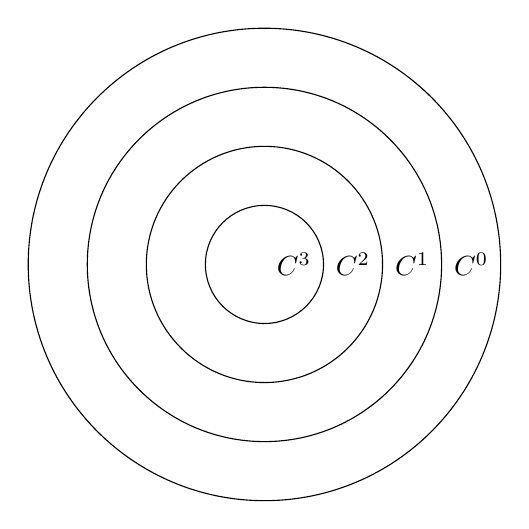
\begin{tikzpicture}
        % Definizione dei raggi dei cerchi
        \def\rmax{3} % Raggio massimo
        \def\step{0.75} % Passo di riduzione tra i cerchi

        % Disegno dei cerchi concentrici
        \foreach \i in {0,1,2,3} {
            \draw (0,0) circle (\rmax-\i*\step);
        }

        % Posizionamento delle etichette
        \node at (\rmax-0.5*\step, 0) {$C^0$};
        \node at (\rmax-1.5*\step, 0) {$C^1$};
        \node at (\rmax-2.5*\step, 0) {$C^2$};
        \node at (\rmax-3.5*\step, 0) {$C^3$};

    \end{tikzpicture}
\end{center}
E insomma, ok, ma la domanda che viene posta è, ESISTONO FUNZIONI DERIVABILI TALI CHE LA LORO DERIVATA NON APPARTIENE ALL'INSIEME $C^1$???
\newpage
\subsection{Funzioni SELVAGGIAMENTE OSCILLANTI}
Prendiamo una funzione discontinua in 0.

Prendiamo $u(x)=x\sin{\frac{1}{x}}$, con $x>0$, la cui derivata è $\sin{\frac{1}{x}}-x\cos{\frac{1}{x}}(x^{-2})=\sin{\frac{1}{x}}-\frac{1}{x}\cos{\frac{1}{x}}$ e non sappiamo se è derivabile. Inoltre la estendiamo definendola in 0, dunque $u(0)=0$ L'unico modo per capirlo (oltre a disegnarla), è fare il rapporto incrementale, dunque, chiamando $u(x)$ questa funzione derivata, consideriamo il suo rapporto incrementale, ossia
\begin{equation*}
    \frac{u(h)-u(0)}{h}=\sin{\frac{1}{h}}
\end{equation*}
Questa funzione però non ha limite per $h \to 0$, dunque la funzione NON è derivabile!!
\\
Se invece scriviamo $x^{1+\frac{1}{2}}\sin{\frac{1}{x}}$, allora avremo $\frac{u(h)-u(o)}{h}=\frac{h^{1+\frac{1}{2}}\sin{\frac{1}{h}}}{h}=\sqrt{h}\sin{\frac{1}{h}}$, che tende a 0, ossia $\sqrt{h}\sin{\frac{1}{h}} \to 0$.
\begin{center}
    \textbf{\textit{Miglioriamo adesso la funzione 1, ossia $\sin{\frac{1}{x}}-\frac{1}{x}\cos{\frac{1}{x}}$}}
\end{center}
Consideriamo una funzione $\frac{3}{2}x^{\frac{1}{2}}\sin{\frac{1}{x}}+x^{\frac{3}{2}}\cos{\frac{1}{x}}(-\frac{1}{x^2})$
\\
Dunque, se considero
$\begin{cases}
    x^{\frac{3}{2}}\sin{\frac{1}{x}}, \,\,\, \mbox{con} \,\,\, x>0 \\
    0 \,\,\, \mbox{con} \,\,\, x=0
\end{cases}$
Allora non ha una derivata continua.
\\
Queste funzione, che possiamo ricordare come \virgolette{selvaggiamente oscillanti}, perchè oscillano veramente tanto, sono l'unico tipo di funzioni che hanno derivata discontinua
\subsection{Teorema di Darboux}
Sia $f:[a,b] \to \R$ derivabile.
\\
Supponiamo che $f'(a) < f'(b)$.
\\
Allora, $\forall \lambda \in [f'(a),f'(b)], \,\,\, \exists \,\, \xi \in (a,b)$ tale che $f'(\xi)=\lambda$.
\\
in analogia con il teorema dei valori intermedi.
\\
\begin{center}
    \textbf{\textit{Dimostrazione}}
\end{center}
Sia $g(x)=f(x)-\lambda x$
Allora:
\begin{align}
    g'(a)=f'(a)-\lambda < 0 \\
    g'(b)=f'(b)-\lambda > 0
\end{align}
Mostro ora che se una funzione $g$ è tale che $g'(a) \leqslant 0$ e $g'(b) \geqslant 0$, allora $\exists \xi \in (a,b)$ tali che $g'(\xi)=0$.
\\
Infatti 
\begin{equation}
    \mbox{Weierstrass} \,\,\,\,\,\Longleftrightarrow \,\,\,\,\,\, \exists \,\,\,\, \xi \mbox{estremante} \in (a,b), \,\,\,\,\,\, \mbox{tale che}\,\,\,\,\,\, g'(\xi)=0
\end{equation}
Ma $\xi \neq a$ e $\xi \neq b$.\\
Supponiamo che $g'(a) < 0$, allora
\begin{equation}
    \lim_{h \to 0^+}\frac{g(a+h)-g(a)}{h}<0
\end{equation}
dunque $a$ non è un minimo, altrimenti $g'(a) \geqslant 0$.
\\
Analogamente $b$ non è un massimo, dunque almeno uno dei due punti sta all'interno.






\subsection{Criterio di Monotonia}
\begin{center}
    \textbf{\textit{1.}}
\end{center}
Se $f$ derivabile in $(a,b)$ e se $f'(x)>0$ per $x \in (a,b)$, allora $f$ è crescente.
\\
Se $x > y$ con $x,y \in (a,b)$, scriviamo $f(x)=f(y)+f'(\xi)(x-y)$, con $\xi \in (y,x)$, dunque 
$\begin{cases}
    x-y > 0 \\
    f'(\xi) > 0
\end{cases}$, e allora
$f(x) > f(y)$, dunque la funzione è crescente
\begin{center}
    \textbf{\textit{NOTA}}
\end{center}
Ricordiamoci che, se $f'(x) \geqslant 0 \Longrightarrow f \,\,\, \mbox{crescente}$, se invece $f'(x) >0 \Longrightarrow f \,\,\, \mbox{strettamente crescente}$
\begin{center}
    \textbf{\textit{2.}}
\end{center}
Se $f$ è crescente $\Longrightarrow f'(x) \geqslant 0$
\\
Consideriamo il rapporto incrementale, ossia $f'(x)=\lim_{h \to 0}\frac{f(x+h)-f(x)}{h}$ e $\frac{f(x+h)-f(x)}{h} \geqslant 0$
$\begin{cases}
    \mbox{per} \,\,\, h>0, \,\,\, \frac{f(x+h)-f(x)}{h}>0 \\
    \mbox{per} \,\, h<0, \frac{f(x+h)-f(x)}{h} >0
\end{cases}$
Il secondo caso è maggiore di zero perchè sia il denominatore che il numeratore sono minori di zero.
\\
Concludiamo dunque che vale la relazione $f'(x)>0 \Longrightarrow f \,\,\, \mbox{crescente}$
\newpage
\subsection{Convessità e concavità}
Un insieme $E \in \R$, o $\R^2,\R^3...$ è convesso se $\forall \,\, x,y \in E$, la linea che congiunge $x$ e $y$ è contenuta \underline{geometricamente} nello stesso insieme
\begin{center}
    \textbf{\textit{Definizione}}
\end{center}
Una funzione $f: (a,b) \to \R$ è convessa \underline{SE}:
\begin{center}
    \textbf{\textit{\hl{1.}}}
\end{center}
$\forall \,\, x,y \in (a,b)$ vale che, $\forall \,\, \lambda \in [0,1]$, allora
\begin{equation*}
    f(\lambda x - (1-\lambda)y) \leqslant \lambda f(x) + (1-\lambda)f(y)
\end{equation*}
Dunque l'\textit{\textbf{epigrafico}} di $f(x)$, ossia l'insieme dei punti ($\alpha, \beta$) tali che $\beta > f(\alpha)$ è \textbf{convesso}.
\begin{center}
    \textbf{\textit{\hl{2.}}}
\end{center}
Se $f$ è derivabile in $(a,b)$:
\begin{itemize}
\item $f$ è convessa se $\forall \,\, x,y \in (a,b)$, allora $f(y) \geqslant f(x)+f'(x)(y-x)$
\end{itemize}
\begin{center}
    \textbf{\textit{\hl{3.}}}
\end{center}
Se $f$ derivabile due volte (ossia $\exists \,\,\, f^{''} : [a,b] \to \R$, allora $f$ è convessa se $f^{''}(x) \geqslant 0$.
\subsubsection{Definizione di concavità}
$f$ è \underline{concava} se $-f$ è convessa 
\begin{center}
    \textbf{\textit{Esercizio}}
\end{center}
Trovare una funzione tale che $f \in C^1(\R) - C^2(\R)$, cioè che appartiene a $C^1$ ma non a $C^2$
\subsubsection{Proposizione}
Se $f$ è derivabile, allora:
\begin{itemize}
    \item $\textbf{1} \Longleftrightarrow \textbf{2}$ (dimostrazione omessa)
    \item $\textbf{2} \Longleftrightarrow \textbf{3}$
\end{itemize}
\begin{center}
    \textbf{\textit{Dimostriamo la seconda}}
\end{center}
Mostriamo che, se $f$ soddisfa la proprietà \textbf{2}, allora $f'(x)$ è una funzione crescente (al che concludiamo poi che $f^{''}\geqslant 0$ per il criterio di monotonia).
\\
Dunque,  prendiamo $x<y$, con $x,y \in (a,b)$.
\\
Sappiamo che:
\begin{equation}
\begin{cases}
    f(y) \geqslant f(x) + f'(x)(y-x) \\
    f(x) \geqslant f(y)+f'(y)(x-y)
\end{cases}
\end{equation}
Da cui dunque $f(x)+f(y) \geqslant f(x)+f(y)+f'(x)(y-x)+f'(y)(x-y)$ \\
Allora $0 \geqslant (f'(x)-f'(y))(y-x)$, allora $f'(y)-f'(x) \geqslant 0$, cioè $f'(y) \geqslant f'(x)$, dunque $f'$ è crescente.
\\
Se allora $f'$ è crescente, per il criterio di monotonia, $f^{''} \geqslant 0$
\newpage
\begin{center}
    \textbf{\textit{Viceversa}}
\end{center}
Sappiamo che, se $f^{''} \geqslant 0$, allora $f' $ è crescente.
\\
Ora, $f(y)=f(x)+f'(\xi)(y-x)$ per Lagrange.
\\
Abbiamo 2 CASI per $f'$ crescente:
\begin{itemize}
    \item Se $x<y$, $\xi \in (x,y)$, e allora $f'(\xi) \geqslant f'(x)$, allora $f(y) \geqslant f(x) + f'(x)(y-x)$
\end{itemize}
ANALOGAMENTE:
\begin{itemize}
\item Se $y<x$, $\begin{cases}
    y-x < 0 \\
    f(y)=f(x)+f'(\xi)(y-x)
\end{cases} \Longrightarrow f(y) \geqslant f(x)+f'(x)(y-x)$
\end{itemize}
\subsection{Principio del minimo}
Sia $f \in C^2([a,b])$, sia $x_0 \in (a,b)$, allora, se $f'(x_0)=0$ e $f^{''}(x_0)>0$, allora $x_0$ è un \underline{minimo locale}, cioè $\exists \,\,\, \varepsilon >0$ tale che $x_0$ è un minimo assoluto di $f: (x_0- \varepsilon; x_0+\varepsilon) \to \R$
\\
\begin{itemize}
\item Se invece $f^{''}<0$ e valgono le stesse condizioni, allora $x_0$ è un massimo
\end{itemize}
\begin{center}
    \textbf{\textit{Dimostrazione}}
\end{center}
Se $f^{''}(x)>0$, allora $\exists$ un intorno di $x_0 (I(x_0))$ dove $f^{''}>0$, poiché $f^{''} \in C^0((a,b))$ (per il teorema di permanenza del segno).
\\
Chiamo allora $(x_0-\varepsilon; x_0+ \varepsilon)$ un intorno dove $f^{''}>0$.
\\
In questo intorno avremo che $f'$ è crescente (perchè $f^{''}>0$).
\\
Dunque, se $x \in (x_0-\varepsilon; x_0+\varepsilon$), $f(x)=f(x_0)+f'(\xi)(x-x_0)$, e dunque abbiamo ulteriori due casi:
\begin{itemize}
    \item $x-x_0 >0$, allora $f'(\xi) \geqslant f'(x_0) =0 \Longrightarrow f(x) \geqslant f(x_0)$
    \item $x-x_0<0$, allora $f'(\xi) \leqslant f'(x_0)=0 \Longrightarrow f'(\xi)(x-x_0) \geqslant 0$
\end{itemize}
\subsection{Flessi}
\begin{center}
    \textbf{\textit{Definizione di flesso orizzontale}}
\end{center}
Sia $f \in C^2([a,b])$ e sia $x_0 \in (a,b)$.
\\
Diremo che $x_0$ è un punto di flesso ORIZZONTALE se $f'(x_0)=0$ e $f^{''}(x)$ \underline{cambia segno} in $x_0$.
\begin{center}
    \textbf{Definizione di flesso obliquo}
\end{center}
Diremo che $x_0$ è un flesso obliquo se $f'(x_0) \neq 0$ e $f^{''}$ cambia segno in $x_0$.
\\
Ad esempio $x^3+x$ presenta un flesso obliquo
\begin{center}
    \textbf{\textit{Definizione di flesso verticale}}
\end{center}
\begin{align*}
    \lim_{h \to 0^+}\frac{f(x+h)-f(x)}{h}= \pm \infty  & \,\,\,\,\,\,\,\,\,\,\,\,\,\,  f^{''}(x_0) > 0 \,\,\,\,\,\,\mbox{per} \,\,\,\,\,\, x < x_0 \\
    \lim_{h \to 0^-} \frac{f(x+h)-f(x)}{h} = \pm \infty  &   \,\,\,\,\,\,\,\,\,\,\,\,\,\,\,    f^{''}(x_0) > 0 \,\,\,\,\,\, \mbox{per} \,\,\,\,\,\, x<x_0  
\end{align*}

Un esempio lo troviamo con
\begin{equation*}
    f(x)=\begin{cases}
        \sqrt{x} \,\,\, \mbox{per} \,\,\, x>0 \\
        -\sqrt{-x} \,\,\, \mbox{per} \,\,\, x<0
    \end{cases}
\end{equation*}

\subsection{Criterio di derivabilità}
Sia $f:(a,b) \to \R$ derivabile in $(a,b) \,\, \backslash \,\, \{x_0\}$, sia $x_0 \in (a,b)$.
\\
Se esistono i seguenti limiti:
\begin{align*}
    \lim_{x \to x_0^+}f'(x)=f'(x_0^+) \\
    \lim_{x \to x_0^-}f'(x)=f'(x_0^-)
\end{align*}
e inoltre $f'(x_0^+)=f'(x_0^-)$, allora $f$ è derivabile in $x_0$
\begin{center}
    \textbf{\textit{Viceversa}}
\end{center}
Se $f'(x_0^+) \neq f'(x_0^-)$, $f$ NON è derivabile in $x_0$

\begin{center}
    \textbf{\textit{Dimostrazione}}
\end{center}
Calcoliamo il rapporto incrementale $\frac{f(x_0+h)-f(x_0)}{h}$, con $h>0$ sarà $=f'(\xi_h)$, e, per Lagrange, il punto $\xi_h \in (x_0, x_0+h)$, dunque $f'(\xi_h) \to f'(x_0^+)$.
\\
Se sciaguratamente $h<0$, $\frac{f(x_0+h)-f(x_0)}{h}=f'(\mu_h)$, con $\mu_h \in (x_0+h, x_0)$, allora $f'(x_0^+)=f'(x_0^-)$.
\\
Adesso, se $f'(x_0^+)=f'(x_0^-)$, nel caso in cui entrambi i valori $\in \R$, allora $f$ sarà derivabile nel punto $x_0$.
\\
Se invece sono diversi, a prescindere che appartengano o meno a $\R$, allora $f$ non è derivabile.
\subsection{Teorema di De L'Hospital}
\begin{itemize}
    \item Siano $f,g: (a,b) \to \R$ e sia $x_0 \in (a,b)$
    \item Siano $f,g$ derivabili in $(a,b)$
    \item Siano $f(x),g(x) \to 0$ quando $x \to x_0$
    \item Sia $g'(x) \neq 0 \forall \,\,\, x\in (a,b)$
    \item Sia $\lim_{x \to x_0}\frac{f'(x)}{g'(x)}=l \in \tilde{\R}$
\end{itemize}
Allora $\lim_{x \to x_0}\frac{f(x)}{g(x)}=\lim_{x \to x_0}\frac{f'(x)}{g'(x)}$
\begin{center}
    \textbf{\textit{Dimostrazione}}
\end{center}
Poniamo 
\begin{equation}
    \frac{f(x)}{g(x)}=\frac{\overline{f}(x)}{\overline{g}(x)}
\end{equation}
dove
\begin{equation}
    \overline{f}(x)=\begin{cases}
        f(x) \,\,\,\,\,\,\,\,\,\,\,\,\, x \neq x_0 \\
        0  \,\,\,\,\,\,\,\,\,\,\,\,\, x=x_0
    \end{cases}
    \end{equation}
    e
    \begin{equation}
        \overline{g}(x)=\begin{cases}
            g(x) \,\,\,\,\,\,\,\,\,\,\,\,\, x \neq x_0 \\
            0 \,\,\,\,\,\,\,\,\,\,\,\,\, x = x_0
        \end{cases}
    \end{equation}
Allora avremo che
\begin{equation}
    \frac{f(x)}{g(x)}=\frac{\overline{f}(x)-\overline{f}(x_0)}{\overline{g}(x)-\overline{g}(x_0)}=\frac{\overline{f'}(\xi)}{\overline{g'}(\xi)}
\end{equation}
dove $\xi \in (x_0, x)$ o $\xi \in (x, x_0)$. Quest'ultimo passaggio si comprende solo alla luce del lemma di cauchy (occhio!).
\\
Adesso, se $x \to x_0$, allora $\xi \to x_0$, dunque
\begin{equation}
    \frac{f(x)}{g(x)}=\frac{\overline{f'}(\xi)}{\overline{g'}(\xi)}=\frac{f'(\xi)}{g'(\xi)} \to l
\end{equation}
\newpage
\subsubsection{Osservazioni sul teorema di De L'Hospital (o fatti)}
\begin{itemize}
    \item La dimostrazione (e dunque il teorema) vale anche se $x =a \bigvee b$
    \item Il teorema (ma non la dimostrazione) vale anche nel caso di $\lim_{x \to +\infty}\frac{f(x)}{g(x)}$ (con il cambio di variabile $t=\frac{1}{x}$)
    \item Il teorema vale anche nel caso $\frac{\infty}{\infty}=\frac{f}{g}$ (ma dimostrarlo è molto complicato)
    \item Se $f,g \to +\infty$, potremmo scrivere $\frac{f}{g}=\frac{\frac{1}{g}}{\frac{1}{f}}=\left[\frac{0}{0}\right]$
\end{itemize}
\subsection{San Taylor (Teorema di Taylor)(Sviluppo di Taylor)}
\subsubsection{Introduzione all'errore}
    \begin{center}
        \textbf{\textit{I resti di Peano}}
    \end{center}
    \begin{enumerate}
        \item \textbf{\textit{(o-piccolo)}}
        \\
        Date le funzioni $f,g: (a,b) \to \R$, con $x_0 \in (a,b)$, diremo che $f=o(g)$, ossia \virgolette{$f$ è un o-piccolo di $g$} SE:
        \begin{itemize}
            \item $\lim_{x \to x_0}\frac{f(x)}{g(x)}=0$, qualora $g(x) \neq 0$ in un $I(x_0)$
            \item $\forall \,\,\,\, \varepsilon>0$ $\exists \delta > 0$ tale che, se $x \in (x_0-\delta; x_0+\delta)-\{x_0\}$, allora
            \begin{equation}
                |f(x)| \leqslant \varepsilon|g(x)|
            \end{equation}
        \end{itemize}
        \item \textbf{\textit{(O-grande)}} \\
        Nelle ipotesi precedenti, $f=O(g)$, cioè $f$ è un O-grande di $g$, se $\exists k>0$ e $\exists \delta > 0$ tale che, se $x \in (x_0-\delta, x_0+\delta)-\{x_0\}$, allora 
        \begin{equation}
            |f(x)| \leqslant k|g(x)|
        \end{equation}
    \end{enumerate}
\begin{center}
    \textbf{\textit{Osservazioni IMPORTANTI NON SKIPPARE}}
\end{center}
\begin{enumerate}
    \item o-piccolo ha due definizioni equivalenti, se $g(x) \neq 0$ (per $x \neq x_0)$, ma la seconda è più generale
    \item La definizione di O-grande non ha alcuna limitazione, ad esempio $sin(x)=O(1)$, infatti $sin(x) \leqslant k \cdot 1$, cioè
    \begin{center}
        O-grande \,\,\,\,\,\,\,\, $\Longleftrightarrow$ $f$ è paragonabile, ma non più grande di $g$, almeno localmente
    \end{center}
    \begin{center}
    \end{center}
\end{enumerate}
\begin{center}
    \textbf{\textit{Osservazioni sull'o-piccolo IMPORTANTE NON SKIPPARE}}
\end{center}
    \begin{enumerate}
        \item La definizione di o-piccolo non è ben posta, questo perchè il punto $x_0$ in cui facciamo il limite è assente nella definizione, ma vedremo che inizieremo a trattare solo $x_0=0$ quindi questo problema diciamo che scomparirà
        \item $o(g)$, in generale, non è una funzione, è un INSIEME DI FUNZIONI, ad esempio \begin{itemize}
            \item $x^3=o(x^2)$ in $x=0$, ed è vero, perchè $\frac{x^3}{x^2} \to 0$, ma anche $x^4=o(x^2)$
        \end{itemize}
        Cioè o-piccolo è l'insieme di funzioni
        \begin{equation}
            o(g)=\{g: (a,b) \to \R \,\, | \,\, \frac{f(x)}{g(x)} \to 0 \,\,\,\,\, (x \to x_0)\}
        \end{equation}
        Dunque l'abuso di notazione che facciamo è che, quando scriviamo $o(g)$, intendiamo l'insieme delle generiche funzioni o-piccolo di quella determinata $g$.
        \item $f=o(g)$ \underline{non} è una scrittura simmetrica, cioè non ha senso dire $o(g)=f$ (tant'è che potremmo usare $f \in o(g)$, ma sarebbe scomodo nelle applicazioni)
    \end{enumerate}
    \subsubsection{Proprietà degli o-piccoli}
    Analizziamo le proprietà degli o-piccoli in un caso particolare e generale allo stesso tempo, cioè nel caso di monomi della forma $X^n$ considerati sempre nel punto $x=0$:
    \begin{enumerate}
        \item $x^n=o(x^m)$ se $n > m$
        \item $c \cdot \,o(x^n)= o (cx^n)=o(x^n)$ , $\forall \,\,\, c \neq 0$, con $c$ costante
        \item $x^n \,\, o(x^m) = o(x^{n+m})=x^m \,\, o(x^n)$
        \item $o(x^n+x^m)=o(x^m)$, con $n \geqslant m$
    \end{enumerate}
    \begin{center}
        \textbf{\textit{Dimostrazione}}
    \end{center}
\begin{enumerate}
    \item $n > m$, allora $\frac{x^n}{x^m}=x^{n-m} \to 0$
    \item $c \,\, o(x^n)=o(x^n) \,\,\,\,\,\, \Longleftrightarrow \,\,\,\, \begin{cases}
        c \,\cdot\, o(x^n) \subset o(x^n) \\
        c \,\cdot\, o(x^n) \supset o(x^n)
    \end{cases}$
    \begin{center}
        ($\Longrightarrow$)
    \end{center}
    Se $f \in c \cdot o(x^n) \Longrightarrow \frac{f(x)}{x^n}=\frac{f(x)}{c \cdot x^n}\cdot c \to$ (limitata) $\to$ 0
    \begin{center}
        ($\Longleftarrow$)
    \end{center}
    (Lasciata per esercizio)
    \item $f \in x^n o(x^m)$, ossia 
    \begin{equation}
   f=x^n\,\cdot\,g, \,\,\,\,\,\,\, \mbox{con} \,\,\,\,\,\,\, g \in \,\, o(x^m) \,\, \Longrightarrow \frac{f(x)}{x^{n+m}}=\frac{x^n g(x)}{x^{n+m}}=\frac{g(x)}{x^m} \to 0 \Longrightarrow x^n o(x^m) \subset o(x^{n+m})
    \end{equation}
    \item ($\subset)$ $f \in o(x^n+x^m)$, quindi $\frac{f(x)}{x^m}=\frac{f(x)}{x^n+x^m} \frac{x^n+x^m}{x^m} =(x^{n-m}+1)\to 0$ 
\end{enumerate}
\begin{center}
    \textbf{\textit{Notazione (già vista) (tilde)}}
\end{center}
$f \texttildelow g $ (in $x_0$) se $\frac{f(x)}{g(x)} \to 1$ OPPURE se
\begin{equation}
    f(x)=g(x)+o(g(x))
\end{equation}









    
\section{Teorema di Taylor vero e proprio}
\subsection*{Notazione e Teorema di Taylor con resto di Peano}

\subsubsection*{Notazione}
Se \( f \sim g \iff \lim_{x \to x_0} \frac{f(x)}{g(x)} = 1 \)

\subsection*{Proposizione}
\( f \sim g \Longleftrightarrow f(x) = g(x) + o(g(x)) \quad \text{(in } x_0 \text{)} \)

\begin{center}
{\textbf{\textit{Dimostrazione}}}
\end{center}
\begin{center}
    $\Longrightarrow$
\end{center}
\[
f \sim g \Rightarrow \lim_{x \to x_0} \frac{f(x)}{g(x)} = 1
\]
\[
\Rightarrow \lim_{x \to x_0} \left( \frac{f(x)}{g(x)} - 1 \right) = 0 \Rightarrow \lim_{x \to x_0} \frac{f(x) - g(x)}{g(x)} = 0
\]
\[
\Rightarrow f(x) = g(x) + o(g(x)) \Rightarrow \frac{f(x)}{g(x)} = 1 + \frac{o(g(x))}{g(x)} 
\Rightarrow \lim_{x \to x_0} \frac{f(x)}{g(x)} = \lim_{x \to x_0} 1 + \frac{o(g(x))}{g(x)} = 1 + 0 = 1 \quad \blacksquare
\]
\begin{center}
    $\Longleftarrow$
\end{center}
Se $f(x)=g(x)+o(g(x))$, allora avrò che
\begin{equation}
    \frac{f(x)}{g(x)}=1+\frac{o(g(x))}{g(x)}
\end{equation}
Faccio il limite per $x \to x_0$ e ottengo:
\begin{equation}
    \lim_{x \to x_0}\frac{f(x)}{g(x)} \to 1+0 =1
\end{equation}
\subsection*{Teorema del Polinomio di Taylor con resto di Peano}
Sia \( f : (a, b) \to \mathbb{R} \quad x_0 \in (a, b) \)

Se \( f \in C^n([a, b]) \), allora:
\[
f(x) = T_n^{x_0}(x) + o((x - x_0)^n)
\]
dove:
\[
T_n^{x_0}(x) = \sum_{k = 0}^{n} \frac{f^{(k)}(x_0)}{k!} (x - x_0)^k
\]

\subsubsection*{Dimostrazione}
Considero:
\[
\lim_{x \to x_0} \frac{f(x) - T_n^{x_0}(x)}{(x - x_0)^n} = l \quad \text{e voglio dimostrare che } l = 0
\]
\[
\Rightarrow f(x) - T_n^{x_0}(x) = o((x - x_0)^n)
\]

Applico il teorema di de l'Hôpital a:
\[
\lim_{x \to x_0} \frac{f(x) - f(x_0) - f'(x_0)(x - x_0) - \dots - \frac{f^{(n-1)}(x_0)}{(n-1)!}(x - x_0)^{n-1}}{(x - x_0)^n}
\]

\[
= \lim_{x \to x_0} \frac{f^{(n)}(x) - f^{(n)}(x_0)}{n!} = 0
\]

\[
\Rightarrow f \in \mathcal{C}^n([a, b]) \quad \blacksquare
\]

\newpage
\subsection{Teorema di Taylor con resto di Lagrange}
Si è sotto le stesse ipotesi del teorema di Taylor con resto di Peano, ma stavolta consideriamo $f \in C^{n+1}((a,b))$.
\begin{equation}
    f(x)=T_{n,x_0}(x)+\frac{f^{n+1}(\xi)(x-x_0)^{n+1}}{(n+1)!}, \,\,\,\,\,\,\,\,\,\,\,\,\,\, \mbox{con} \,\,\,\,\,\,\,\, \xi \in (a,b)
\end{equation}

\begin{center}
    \textbf{\textit{Dimostrazione (più uno sketch che una dimostrazione completa)}}
\end{center}
Sia $x<x_0$ (non essenziale, ma semplifica i conti).
\begin{equation}
    \frac{f(x)-T_{n,x_0}(x)}{(x-x_0)^{n+1}}=\frac{f^{(n+1)(\xi)}}{(n+1)!}
\end{equation}
Mi metto in $x_0=0$, allora
\begin{equation}
\frac{f(x)-T_{n,x_0}(x)}{x^{n+1}}=\frac{f'(\xi_1)-T'_{n,x_0}(\xi_1)}{(n+1)(\xi_1)^n}=(\mbox{iterando})=\frac{f^n(\xi_2)-T^N(\xi_2)}{(n+1)n(\xi_2)^{n-1}}
\end{equation}





























\newpage
\section{Serie numeriche}
Cos'è una serie numerica??
\\
Sia $\{a_n\}$ una successione numerica.
\\
Pongo $S=a_0+a_1+...+a_n=\sum_{k=0}^na_k$, che chiameremo \textit{somma parziale n-esima}.
\\
Chiamiamo adesso serie di $\{a_n\}$ il limite $\lim_{n \to +\infty}S_n=\sum_{n \geqslant 0}a_n=\sum a_n$
\\
\begin{center}
    \textbf{\textit{Osservazione}}
\end{center}
La definizione è mal posta, ma significa che la serie di $a_n (\sum a_n)$ però:
\begin{enumerate}
    \item $\exists$ in $\R$ (se il limite esiste e converge)
    \item $\exists$ ma è uguale a $\pm \infty$
    \item Non esiste
\end{enumerate}
Ora, se vale 1 la serie converge, se vale 2 o 3 diremo che la serie NON converge.
\\
Se vale 2 allora la serie diverge.
\\
Se vale la 3 allora la serie è irregolare.

\subsection{Serie di Grandi}
$a_n=(-1)^n$, $S=\sum_{n \geqslant 0}a_n$.
\\
Osserviamo che se mettiamo $-S=-\sum (-1)^n= \sum (-1)^{n+1}=-1+S$.
\\
Capiamo quindi che ci viene $S=\frac{1}{2}$, ma capiamo da soli che non ha molto senso, dove sta l'inghippo??
\\
L'inghippo sta nel fatto che noi abbiamo utilizzato come numero noto $S$ senza sapere in realtà se esiste o meno, noi nel dubbio lo abbiamo usato, e questo ha portato a questo banale errore, per cui dobbiamo in realtà osservare che $S$ può valere 0 oppure 1, ma questo non possiamo definirlo in una somma infinita, perchè non ci fermiamo mai, quindi $S$ rimarrà tranquillamente un oggetto indefinito.
\begin{center}
    \textbf{\textit{Esempio 2}}
\end{center}
Consideriamo adesso invece la successione $a_n=\frac{1}{2^n}$, da cui $\sum a_n=1$, perchè infatti $S_n=\sum_{k=1}^n \frac{1}{2^n}=\left(\sum_{k=0}^n \frac{1}{2^{n-1}}- 1\right)=\sum_{k=0}^n (\frac{1}{2})^k-1=\frac{1-(\frac{1}{2}^{n+1})}{1-\frac{1}{2}}= 2-1 = 1$

\vspace{15pt}
\hrule
\vspace{15pt}

\begin{center}
    \textbf{\textit{Lemma}}
\end{center}
\subsection{Criterio necessario di convergenza}
Se $\sum a_n \in \R \Longrightarrow a_n \to 0$, cioè se la serie di $a_n$ è un numero reale, allora la successione $a_n$ deve tendere a 0, vediamo di dimostrare il perchè.
\\
\begin{center}
    \textbf{\textit{Dimostrazione}}
\end{center}
Se $\sum a_n \in \R \Longrightarrow S_n=\sum_{k=0}^r a_k \to S \in \R$, ma allora $S_n-S_{n-1}=a_n=S-S=0$
\begin{center}
    \textbf{\textit{ IL VICEVERSA \'E FALSO (vediamo che $\sum \frac{1}{n}$})}
\end{center}
\newpage
\begin{center}
    \textbf{\textit{Fatto $\left(\,\,\sum \frac{1}{n} \,\,\,\,\mbox{non converge}\,\,\right)$}}
\end{center}
$a_n=\frac{1}{n} \to 0$. \\
{[RAA]} Se $\sum a_n \in \R$, $S_n=\sum_{k=1}^h \frac{1}{k} \to S$, allora $S_{2k}-S_{k}=\sum_{k=n+1}^{2n} \frac{1}{k}$, e dunque $\sum_{k=n+1}^{2n} \frac{1}{k} \geqslant \frac{1}{2n} \cdot n=\frac{1}{2}$, ma questo è impossibile!!
\begin{center}
    \textbf{\textit{Osservazione: criterio di Cauchy per le serie numeriche}}
\end{center}
$\forall \,\,\, \varepsilon > 0 \,\,\, \exists \,\,\, N \in \N$ tale che, se $n \geqslant m \geqslant N$, allora \,\,\,\,\,\,$|\sum_{k=m+1}^n a_k|< \varepsilon $

\subsection{Algebra delle serie}
\begin{enumerate}
    \item Se $\sum a_n \in \R$ e $\sum b_n \in \R$, allora $\sum a_n + \sum b_n = \sum (a_n+b_n)$, e chiaramente converge
    \item Se $c \in \R$, allora $c\sum a_n=\sum c \,\, a_n \in \R$
\end{enumerate}
\begin{center}
    \textbf{\textit{Dimostrazione}}
\end{center}
\begin{enumerate}
    \item  $S_n=\sum a_n$, sia $I_n=\sum b_n$. Allora $S_n+I_n=(a_1+b_1)+...+(a_n+b_n)$
    \item Consideriamo $\sum a_n= a_0+a_1+...+a_n$, per cui $c \sum a_n = c (a_0+a_1+...+a_n)= c\,\,a_0+c\,\,a_1+,,,+c\,\, a_n= \sum c \,\, a_n$, e inoltre $\sum c \, a_n \in \R$, perchè i reali sono un insieme chiuso rispetto alla moltiplicazione, dunque se $c \in \R$ e $\sum a_n \in \R$ per ipotesi, allora il prodotto deve appartenere ai reali, dunque abbiamo una serie che converge anche nel caso di prodotto per uno scalare.
\end{enumerate}
\begin{center}
    \textbf{\textit{Esercizio}}
\end{center}
Consideriamo la serie $\sum_{n \geqslant 0} \sin({n})$ non converge, infatti $\sin({n}) \nrightarrow 0$ (che è difficile da dimostrare, ma ci si può arrivare intuitivamente dal fatto che sì, è vero che si annullano i termini positivi e negativi, ma proprio come abbiamo visto per la serie di grandi, abbiamo differenti risultati in base a dove ci fermiamo a sommare, per cui non sappiamo effettivamente, fermandoci DEFINITIVAMENTE (ossia dopo un certo \virgolette{tempo} $N$, se effettivamente la serie converge, dunque diamo per assodato che non converga)
\begin{center}
    \textbf{\textit{Definizione di Definitivamente (Rinfrescata)}}
\end{center}
Una proprietà $P(n)$, con $n \in \N$, vale \underline{definitivamente} se $\exists \,\, N >0$ tale che $P(n)$ vale se $n > N$
\begin{center}
    \textbf{\textit{Osservazione}}
\end{center}
Se $\{a_n\}_{n \geqslant 0}$, $\{\tilde{a_n}\}_{n \geqslant 10}$, allora $a_n = \tilde{a_n}$.
\\
Quello che vogliamo dire con questa osservazione è che la serie $\sum a_n$ ha esattamente la stessa natura di $\sum \tilde{a_n}$, infatti $\sum_{k=0}^n a_k = \sum_{k=11}^n a_k + A$

 \vspace{15 pt}
 \hrule
 \vspace{15 pt}
 \begin{center}
     \textbf{\textit{RICORDA!!!}}
 \end{center}
I primi termini di una serie non influenzano l'andamento della serie stessa, ne cambiano solo il valore numerico, cioè, se una serie deve convergere DEFINITIVAMENTE, puoi stare tranquillo che converge, e lo farà a prescindere dal valore dei primi termini. \hl{Quindi, se una serie converge o diverge, io posso aggiungergli quello che voglio, ma non cambierò niente a livello di convergenza e/o divergenza, semplicemente cambierò il valore numerico, ma la natura della serie è già fissata}
\\
\vspace{15 pt}
\hrule
\vspace{15 pt}
\begin{center}
    \textbf{\textit{4 serie fondamentali (IMPORTANTE)}}
\end{center}
Troviamo quattro tipologie fondamentali di serie numeriche, analizziamole singolarmente:
\begin{enumerate}
    \item \textbf{Serie Geometrica:} \\
    Sia $q \in \R$, sia $a_n= q^n$, allora \[\sum_{k=0}^{+\infty} q^k\] può prendere due strade:
    \begin{itemize}
        \item \textbf{Converge} a $\frac{1}{1-q}$ se $q \in (-1;1)$
        \item Non converge in tutti gli altri casi
    \end{itemize}
    \item \textbf{Serie Telescopica:} \\
    Sia $\{a_n\}$ una successione. Sia poi $b_n=a_{n+1}-a_n$; allora \[\sum_{n \geqslant 0}b_n= \lim_{n \to +\infty}a_n-a_0\] (abuso di notazione)
    \item \textbf{Serie Armonica Generalizzata:} \\
    Consideriamo la successione $a_n= \frac{1}{n^p} \in \R \,\, \Longleftrightarrow \,\, p>1$, altrimenti \[\sum \frac{1}{n^p}= +\infty\] (se $p \leqslant 1$).
    \item \textbf{Serie numerica di Bertrand:} \\
    Consideriamo i parametri $\alpha, \beta \in \R$ e consideriamo la successione $a_n= \frac{1}{n^\alpha \ln{n}^\beta}$.
    \\
    Dunque, questa serie, come tutte le altre, diverge o converge in base ai valori che i suoi parametri assumono, dunque:
    \begin{itemize}
        \item $\sum a_n \in \R$ (cioè la serie converge) se $\alpha >1 \vee \alpha =1$ e $\beta > 1$
        \item $\sum a_n =+ \infty$ (cioè la serie diverge) se $\alpha < 1 \,\, \vee \,\, \alpha =1$ e $\beta \leqslant 1$
        \\
        (Osservare come $\beta$ entri in gioco solo se $\alpha \leqslant 1$ 
        \end{itemize}

\end{enumerate}
\begin{center}
    \textbf{\textit{Dimostrazione della serie geometrica}}
\end{center}
Abbiamo detto che la serie geometrica, del tipo $\sum a_n$, con $a_n=q^n$, con $q \in \R$, può convergere o divergere, vediamo perchè
\\
\[S_n=\sum_{k=0}^n q^k = \frac{1-q^{n+1}}{1-q}\], e ora vediamo tutti i casi con i valori di $q$:
\begin{itemize}
    \item Se $|q| < 1$, allora $q^{n+1} \to 0$
    \item Se $q = 1$, allora $S_n = n + 1 \to +\infty$
    \item Se $q > 1$, allora $q^{n+1} \to +\infty$, dunque $1-q <0$ e la serie diverge, infatti $S_n \to +\infty$
    \item Se $q \leqslant -1$, allora $q^n$ è indeterminata
\end{itemize}
\newpage
\begin{center}
    \textbf{\textit{Dimostrazione della serie telescopica}}
\end{center}
Abbiamo considerato $b_n=a_{n+1}-a_n$.
\\
Dunque la serie sarà $S_n=b_0+b_1+...+b_n=(a_1-a_0)+(a_2-a_1)+(a_3-a_2)+...+(a_{n+1}-a_n)= a_{n+1}-a_0$
\begin{center}
    \textbf{\textit{Dimostrazione della serie armonica generalizzata, ossia $[\frac{1}{h^p}]$}}
\end{center}
Se $p \leqslant 0$, allora $\frac{1}{h^p} \nrightarrow 0$.
\\
Dunque $\sum \frac{1}{h^p} = +\infty$ per \textit{contronominale} del criterio necessario di convergenza.
\\
Altrimenti, nel caso contrario, se $p > 0$, avremo che $\frac{1}{h^p}$ è decrescente.
\\
Poniamo dunque $a_n=\frac{1}{h^p}$ e sfruttiamo il CCC, dunque:
\begin{equation}
    2^na_{2^n}=\frac{2^n}{2^{hp}}=\left[\frac{1}{2^{(p-1)}}\right]^h
\end{equation}
Pongo allora $q=\frac{1}{2^{p-1}}$ e identifico $q^h$ in una \textbf{serie geometrica}, infatti sappiamo che:
\begin{equation}
    \sum q^h \,\,\,\,\, \mbox{converge} \,\,\,\, \Leftrightarrow \,\,\,\,\,\, |q| < 1 \,\,\,\,\, \Leftrightarrow \,\,\,\, \frac{1}{2^{p-1}}<1 \,\,\, \Longrightarrow p-1 > 0 \Longrightarrow p > 1
\end{equation}.
\\
Poichè:
\begin{equation}
    \sum 2^n a_{2n} < +\infty \Longrightarrow \sum a_n < +\infty \,\,\,\,\ \mbox{per il CCC}
\end{equation}









\newpage
\subsection{Serie a Termini Positivi}
In questo sottocapitolo assumeremo che le successioni siano a termini tutti positivi, dunque che $a_n \geqslant 0 \,\,\, \forall \,\,\, n$
\begin{center}
    \textbf{\textit{Lemma (chiarisce perchè i termini positivi sono importanti)}}
\end{center}
Sia $a_n$ una successione a termini positivi (dunque $a_n \geqslant 0$, allora $\sum a_n$ converge $\Longleftrightarrow \,\, S_n= \sum_{k=0}^n a_k$ è limitata
\begin{center}
    \textbf{\textit{Dimostrazione}}
\end{center}
Osserviamo che, dato che $a_n \geqslant 0$, allora $S_{n+1}=S_n+ a_{n+1} \geqslant S_n$, da cui $a_{n+1} \geqslant 0$, dunque $S_n$ è monotona crescente.
\\
Per il teorema delle successioni monotone, $S_n$ converge al suo $sup$, cioè $S_n \to sup(S_n)$, con $n \in \N$ e $sup \in \tilde{\R}$.
\\
Concludiamo: Se $sup(S_n)=S \in \R$ allora $S_n$ è limitata, e questo equivale a dire che $\sum a_n \in \R$.
\\
\cvd
\begin{center}
    \textbf{\textit{Notazione}}
\end{center}
Diciamo già che $\sum a_n$ converge scrivendo $\sum a_n \in \R$.
\\
Se $\{a_n\}$ è tale che $a_n \geqslant 0$, possiamo scrivere $\sum a_n < +\infty$ invece che $\sum a_n \in \R$

\vspace{15pt}
\hrule
\vspace{15pt}

\begin{center}
  \warning \,\,\, ATTENZIONE \,\,\, \warning
\end{center}
Questa notazione vale solo se parliamo di successioni a termini positivi, negli altri casi perde totalmente di significato

\vspace{15pt}
\hrule
\vspace{15pt}

\begin{center}
    \textbf{\textit{Criterio del confronto}}
\end{center}
Siano $a_n$ e $b_n$ due successioni a termini positivi. Se:
\begin{enumerate}
    \item $a_n \leqslant b_n$ (\underline{anche solo definitivamente})
    \item $\sum b_n < +\infty$
\end{enumerate}
Allora $\sum a_n < +\infty$
\\
Ricordiamoci che possiamo sempre scrivere tutte queste cose aggiungendo definitivamente, perchè come abbiamo detto in precedenza (c'è un RICORDA!!! scritto apposta)
\\
\begin{center}
    \textbf{Dimostrazione}
\end{center}
Chiamo $A_n=a_0+...+a_n$, $B_n=b_0+...+b_n$.
\\
Osserviamo che $2)$ vale $\,\, \Longleftrightarrow \,\, \lim_{n \to +\infty}B_n = B \in \R$.
\\
Ma allora $A_n \leqslant B_n$ (poichè $a_k \leqslant b_k \,\, \forall \,\, k \in \N $).
\\
Dunque $A_n \leqslant B_n \leqslant sup(B_n) =B$, cioè $0 \leqslant A_n \leqslant B_n \,\,\forall \,\, n \in \N$, ossia, $A_n$ è LIMITATA!

\begin{center}
    \textbf{\textit{Vale il viceversa}}
\end{center}
Se infatti $0 \leqslant a_n \leqslant b_n$ e $\sum a_n =+ \infty$, allora anche $\sum b_n = +\infty$
\\
In pratica abbiamo fatto la dimostrazione contronominale del lemma precedente).
\\
\subsubsection{Criterio del confronto asintotico}
Ricordiamoci innanzitutto che $a_n= o(b_n)$ se $\frac{a_n}{b_n} \to 0$, e, più nel dettaglio, se:
\\
$\forall \,\, \varepsilon > 0 \,\, \exists \,\, N \in \N$ tale che $|a_n|<k|b_n|$ (cioè stiamo dicendo che, definitivamente, possiamo mettere a paragone le due successioni).
\\
\begin{center}
    \textbf{\textit{Criterio del confronto vero e proprio}}
\end{center}
Fissiamo $\{a_n\}$ e $\{b_n\}$ successioni, tali che $a_n \geqslant 0$, $b_n \geqslant 0$, e questo $\forall \,\, n \in N$
\begin{enumerate}
    \item Se $a_n=O(b_n)$, se $\sum b_n < +\infty$, anche $\sum a_n < +\infty$
    \item Se $a_n= o(b_n)$, allora $\sum a_n < +\infty \,\, \Longleftrightarrow \,\, \sum b_n < +\infty$, cioè convergono entrambe, sono della stessa natura.
    \item $a_n \texttldelow b_n$, $\sum a_n < +\infty \Longleftrightarrow \sum b_n < +\infty$
    \end{enumerate}
    \\
    \begin{center}
        \textbf{\textit{Dimostrazione}}
    \end{center}
Osserviamo innanzitutto che $1 \Longrightarrow 2$, infatti, se $a_n = o(b_n)$, allora $a_n= O(b_n)$, questo perchè è un O grande con $k= \varepsilon$
\begin{center}
    \textbf{\textit{Dimostrazione del punto 1}}
\end{center}
Se $a_n=O(b_n)$ e $a_n \geqslant 0$, allora $a_n \leqslant k \, b_n$ \underline{definitivamente}.
\\
Inoltre, se $\sum b_n < +\infty$, anche $\sum k \, b_n < +\infty$.
\\
Concludiamo con il teorema del confronto e abbiamo chiuso.
\\
\begin{center}
    \textbf{\textit{Dimostriamo il punto 3 (se 1 implica 2 e abbiamo dimostrato 1, allora 2 è dimostrato)}}
\end{center}
$a_n \texttildelow b_n \,\, \Longirghtarrow \,\, a_n=O(b_n)$ e che $b_n=O(a_n)$.
\\
Per $1$, $b_n=O(a_n) \,\, \Longrightarrow \,\,$ se $\sum a_n < +\infty$, allora $\sum b_n < +\infty$ as well (pure).
\\
\cvd
\begin{center}
    \textbf{\textit{Esempio sul criterio del confronto}}
\end{center}
Consideriamo $a_n=\frac{1}{n^2+1}$, cosa fa la serie $\sum a_n$?
\\
Sappiamo che $a_n \geqslant 0$, sappiamo anche che $a_n \texttildelow \frac{1}{n^2}$, la cui serie converge, perchè $2 > 1$, e abbiamo visto con i quattro tipi che è una armonica generalizzata.

\subsection{Criterio del rapporto e della radice}
Sia $a_n > 0 \,\, \forall \,\, n \in N$, se:
\begin{enumerate}
    \item $\frac{a_{n+1}}{a_n} \to l$ e $l < 1 \,\, \Longrightarrow \,\, \sum a_n < +\infty$
    \\
    Se $l > 1$ sicuramente $\sum a_n = +\infty$
    \item Se $\sqrt[n]{a_n} \to l$ e :
    \begin{itemize}
        \item $l < 1$, allora $\sum a_n < +\infty$
        \item $l > 1$, allora $\sum a_n = +\infty$
    \end{itemize}
\end{enumerate}
\vspace{15pt}
\hrule
\vspace{15pt}
\begin{center}
    \textbf{\textit{NOTA}}
\end{center}
Il caso $l > 1$, dal criterio analogo per le successioni, implica che $a_n \to + \infty$ e dunque $a_n \nrightarrow 0$, dunque $\sum a_n$ NON CONVERGE, ma, dato che $a_n \geqslant 0$, questo vuol dire che $\sum a_n = +\infty$

\begin{center}
    \textbf{\textit{Dimostrazione criterio del rapporto e della radice}}
\end{center}
(Le dimostrazioni sono identiche a quelle viste per gli stessi criteri ma sulle successioni, l'unica differenza è che alla fine bisogna passare alla serie e concludere con il criterio del rapporto. Inoltre è banale osservare che se $l > 1$, in entrambi i casi la serie diverge per il criterio necessario di convergenza)
\\
\begin{center}
    \textbf{\textit{Osservazione}}
\end{center}
Nella lezione precedente si è detto che $\sum \frac{1}{n} \notin \R$.
\\
Ora sappiamo che $\sum \frac{1}{n} = +\infty$, perchè o converge o diverge, e sappiamo che non converge, quindi deve divergere.
\\
\vspace{15pt}
\hrule
\vspace{15pt}
\begin{center}
\subsection{\textbf{\textit{Criterio di condensazione di Cauchy (CCC)}}}
\end{center}
Sia $\{a_n\}$ una successione a termini positivi, tale che decresce e tende a 0, ossia $a_n \searrow 0$ ($a_n \to 0$ e contemporaneamente $a_{n+1} \leqslant a_n$).
\\
Allora $\sum a_n < +\infty \,\, \Longleftrightarrow \,\, \sum 2^na_{2^n} < +\infty$
\begin{center}
    \textbf{\textit{Dimostrazione}}
\end{center}
Chiamiamo $S_n$ le somme parziali di $a_n$, ossia $S_n=a_0+...+a_n$.
\\
Chiamiamo poi $T_n=2^0a_1+2a_2+2^2a_4+2^3a_8+...+2^na_{2^n}$.
\\
\textit{Facciamo ora un calcolo  :}\\
\[S_{2^{n}-1}= a_0+ a_1 + a_2 + a_3 +a_4 + ... + a_7+a_8+...+a_{15}+a_{2^{n-1}}+...+a_{2^n-1}\]
\\
Se stiamo molto attenti, ci accorgiamo che:
\begin{itemize}
    \item $a_1 \leqslant 2^0a_{2^0}$
    \item $a_2+ a_3 \leqslant 2a_2$
    \item $a_4+...+a_7 \leqslant 2^2a_4$
    \item $a_8+...+a_{15} \leqslant 2^3a_8$
    \item $a_{2^{n-1}}+...+a_{2^n-1}$
\end{itemize}
Se $T_n \to T \in \R$ o, equivalentemente $T_n$ è limitata, anche $S_n$ lo è, proprio perchè ogni termine di $S_n$ è minore uguale a ogni termine di $T_n$.
\\
Infatti sia $n \in \N \backslash \{0\}$, $m \leqslant 2^m - 1$, e dunque:
\\
$S_m \leqslant S_{2^n-1}\leqslant a_0+ T_{m-1} \leqslant a_0 + T \in \R$, e questo implica che $\sum a_n < +\infty$
\begin{center}
    \textbf{\textit{[L'altro verso della dimostrazione è analogo, si accorpano i termini e si fa la diseguaglianza con il verso opposto però]}}
\end{center}
Infatti si ottiene alla fine della dimostrazione inversa, che $S_{2^n} \geqslant \frac{1}{2}T_n$, dunque se $S_n \leqslant S \in \R$, allora $T_n$ è, anch'essa, limitata.
\\
\cvd
\begin{center}
    \textbf{\textit{Corollario}}
\end{center}
$\sum \frac{1}{n^p}$ converge, ossia $\sum \frac{1}{n^p} < +\infty \,\, \Longleftrightarro \,\,  \sum \frac{2^n}{(2^n)^p} < +\infty$ (Infatti se $p >0$, se $p \leqslant 0$, $a_n \nrightarrow 0$).
\\
Ma $b_n=\frac{2^n}{(2^n)^p}=\frac{1}{2^{np-n}}=\left[(\frac{1}{2})^{p-1}\right]^n$, se chiamo $\left(\frac{1}{2}\right)^{p-1}=q$, allora ho $\sum b_n = \sum q^n$, che converge $\Longleftrightarrow \,\, q < 1$ (con $q \geqslant 0$).
\\
Verifichiamo che $\left(\frac{1}{2}\right)^{p-1} \,\, \Longleftrightarrow \,\, 2^{p-1} > 1 \,\, \Longleftrightarrow (p-1)\log_2{2} > 0 \,\, \Longleftrightarrow p >1$ (se non capisci guarda i passaggi lentamente che ci si arriva in un attimo, devi applicare il logaritmo in base due a entrambi i membri e arrivi subito a concludere che $p > 1$).
\subsubsection{\textbf{\textit{Come si calcola e riflessione sulla serie di Bertrand}}}
Partiamo da come si calcola la serie di Bertrand, ossia:
\begin{equation}
    \sum \frac{1}{n^\alpha (ln(n))^\beta}
\end{equation}
Adesso, abbiamo tre casi a seconda del valore di $\alpha$, dunque:
\begin{itemize}
    \item $\alpha > 1$, in questo caso la serie \textbf{converge} $\forall \beta$
    \item $\alpha =1$, allora converge se $\beta=1$, diverge se $\beta \leqslant 1$
    \item $\alpha < 1$, allora la serie \textbf{diverge} $\forall \,\,\,\,\, \beta$
\end{itemize}
Consideriamo la successione di Bertrand, ossia $a_n=\frac{1}{n^\alpha \ln{n}^\beta}$.
\\
Ora, se $\alpha > 1$, il logaritmo non ci interessa, perchè entra in gioco quando $\alpha=1$.
\\
Ora, il nostro obiettivo è quello di applicare il CCC, però prima occhio, perchè se $\alpha < 0$, allora per la gerarchia degli infiniti la successione diverge a $+\infty$, dunque non converge, e, siccome $a_n \geqslant 0$, $\sum a_n = +\infty$.
\\
Analizziamo i diversi valori che $\alpha$ può assumere:
\begin{itemize}
    \item Se $\alpha =0$, allora $a_n=\frac{1}{\ln{n}^\beta}$ e la serie diverge, perchè $\frac{1}{n}=o\left(\frac{1}{\ln{n}^\beta}\right)$ e , inoltre $\sum \frac{1}{n}=+\infty$ e, dunque, se sommo o-piccoli di $\frac{1}{n}$, che già diverge, allora continueremo a divergere.
    \\
    Inoltre, se per assurdo $\sum \frac{1}{\ln{n}^\beta} < +\infty \,\, \Longrightarrow \sum \frac{1}{n} < +\infty$ per il criterio del confronto, ma abbiamo dimostrato che $\frac{1}{n}$ diverge, dunque sarebbe una contraddizione.
    \item Se $\alpha > 0$, allora dobbiamo verificare, per applicare il CCC, che la successione sia decrescente (per lo meno definitivamente).
    \\
    Consideriamo allora
    \begin{align*}
        f: \,\, \left[2, +\infty \right) \to \R  \\
        x \mapsto \frac{1}{x^\alpha \ln{x}^\beta}
        \end{align*}
        Dunque, se $f \searrow$ in $\R$, decrescerà anche nei naturali, e dunque anche $a_n \searrow 0$.
        \\
        Verifichiamo allora che \begin{equation*}
            a_{n+1}=f(n+1) \leqslant f(n) = a_n
        \end{equation*}
\end{itemize}
\vspace{15pt}
\hrule
\vspace{15pt}
\begin{center}
    \textbf{\textit{Esercizio che serve nella dimostrazione}}
\end{center}
Calcolare $f'(x)$ e mostrare $f'(x) < 0$ per $x$ molto grandi
\vspace{15pt}
\hrule
\vspace{15pt}
Dunque, dimostrato che la funzione decresce (e quindi la successione), possiamo applicare il CCC, e allora $\sum a_n < +\infty \,\, \Longleftrightarrow \,\, \sum 2^n a_{2^n} < +\infty$.
\\
Calcolo allora $2^na_{2^n}=\frac{2^n}{2^{n\alpha}\ln{2^n}^\beta}=\frac{1}{(2^{\alpha-1}n^\beta) \ln{2}^\beta}$.
\\
Usiamo allora il criterio della radice e osserviamo:
\begin{equation*}
    \sqrt[n]{2^na_{2^n}} \,\,\,\,\texttildelow \,\,\,\,\, \frac{1}{2^{\alpha - 1}}
\end{equation*}
(per il criterio della radice abbiamo usato il fatto che $\sqrt[n]{n^\beta} \to 1$, allora $\sqrt[n]{c} \to 1$ se $c > 0$).
\\
\begin{itemize}
\item Il criterio della radice mi assicura allora che la somma
\begin{equation*}
    \sum 2^n a_{2^n} < +\infty \,\,\,\,\,\,\, \mbox{se} \,\,\,\,\,\,\, \frac{1}{2^{\alpha -1 }} < 1 \,\,\, \Longleftrightarrow \,\,\, \alpha > 1
\end{equation*}
inoltre $\sum 2^n a_{2^n} < +\infty $ (diverge) se $\frac{1}{2^{\alpha -1 }} > 1 \,\,\, \Longleftrightarrow \,\,\, \alpha < 1$.
\item Se poi $\alpha= 1$, allora non ha senso il criterio della radice, però in realtà mi informa che $2^n a_{2^n}=\left(\frac{1}{\ln{2}^\beta}\right)\frac{1}{n^\beta}$, la cui serie converge $\,\, \Longleftrightarrow \,\, \beta > 1$
\end{itemize}
\subsection{Serie di successioni a segno qualunque}
Non sappiamo molto sulle successioni a segno generico, anche perchè fino ad ora abbiamo visto solo serie di successioni che hanno solo termini positivi, il che rendeva più semplice capire se potessero divergere o convergere, e abbiamo visto i diversi criteri e lemmi vari che ci aiutavano.
\\
Adesso però le cose si complicano, vogliamo analizzare le serie di successioni delle quali non abbiamo idea di come la variazione di segno possa risultare, dunque.
\\
Abbiamo DUE FONDAMENTALI CRITERI per questo genere di successioni, il primo è il \textit{criterio di convergenza assoluta}
\subsubsection{Criterio di convergenza assoluta}
\begin{center}
    \textbf{\textit{Definizione}}
\end{center}
Sia $\{a_n\}$ una successione. Diremo allora che $\sum a_n$ converge ASSOLUTAMENTE se $\sum |a_n| < +\infty$.
\vspace{15pt}
\hrule
\vspace{15pt}
\begin{center}
    \textbf{\textit{Osservazione}}
\end{center}
La notazione $\sum a_n < +\infty$ NON \'E PI\'U VALIDA perchè non siamo più nelle condizioni in cui $a_n \geqslant 0$. Se vogliamo usare quella notazione dobbiamo SEMPRE essere sicuri che $a_n \geqslant 0$, altrimenti bocciati e al prossimo appello, dai dai dai.
\vspace{15pt}
\hrule
\vspace{15pt}
\begin{center}
    \textbf{\textit{Criterio di convergenza assoluta}}
\end{center}
Sia $a_n$ una successione. Se $\sum |a_n| < +\infty $, allora $\sum a_n$ converge.
\\
\begin{center}
    \textbf{\textit{Dimostrazione}}
\end{center}
Poniamo due successioni particolari:
\begin{equation*}
    a_n^+=\begin{cases}
        a_n \,\,\,\, \mbox{se} \,\,\,\, a_n \geqslant 0 \\
        0 \,\,\,\, \mbox{se} \,\,\,\, a_n \leqslant 0
    \end{cases}
\end{equation*}
e
\begin{equation*}
    a_n^-=\begin{cases}
        -a_n \,\,\,\, \mbox{se} \,\,\,\, a_n \leqslant 0 \\
        0 \,\,\,\, \mbox{se} \,\,\,\, a_n \geqslant 0
    \end{cases}
\end{equation*}
$a_n^+$ e $a_n^-$ le chiameremo \underline{parte positiva} e \underline{parte negativa} della successione generica $a_n$.
\begin{center}
    \textbf{\textit{Osservazioni}}
\end{center}
Osserviamo innanzitutto che $a_n^+ + a_n^- = |a_n|$, e inoltre, entrambe le successioni sono a termini positivi, matematicamente lo scriviamo $a^\pm \geqslant 0$.
\\
Ancora, osserviamo che vale la diseguaglianza $0 \leqslant a_n^\pm \leqslant |a_n|$, e da qui, per il criterio del confronto, possiamo dire che entrambe convergono, ossia che $\sum a_n^+$ e $\sum a_n^-$ convergono entrambe.
\\
Ma, per l'algebra delle serie numeriche vista all'inizio, se abbiamo due serie che convergono e le sommiamo, allora la somma delle serie deve convergere anch'essa, dunque scopriamo che, essendo $a_n^+ - a_n^- = a_n$, allora $\sum a_n$ convergerà.
\\
\vspace{15pt}
\hrule
\vspace{15pt}
\begin{center}
    \textbf{\textit{Esercizi/Osservazioni}}
\end{center}
\begin{itemize}
    \item Consideriamo $a_n=\frac{(-1)^n}{n^2}\ln{n+1}$, cosa fa la serie $\sum a_n$???
    \\
    Osserviamo innanzitutto che $|a_n|= \frac{\ln{n+1}}{n^2} \texttildelow \frac{\ln{n}}{n^2}= \frac{1}{n^2 \ln^{-1}{n}}$, la cui serie converge, perchè è una serie di Bertrand e 2>1 
    \item Prendiamo invece $a_n=\frac{|sin(n)| \, \ln{n+1}}{n^2} \leqslant \frac{\ln{n+1}}{n^2}$, la cui serie converge perchè, di nuovo $2 > 1$ e, essendo di Bertrand, converge 
    \item \textbf{\textit{Esercizio}}:
    \\
    $a_n= \frac{(-1)^n}{n}$, $|a_n|=\frac{1}{n}$, ma sappiamo che $\sum \frac{1}{n} \, > +\infty$, dunque non possiamo usare il criterio, ma vedremo successivamente che questa serie converge, dunque NON VALE IL VICEVERSA del criterio di convergenza assoluta.
\end{itemize}
\subsection{Criterio di Abel}
Sia $a_n$ una successione tale che $a_n = \varepsilon_n \cdot b_n$ e:
\begin{enumerate}
    \item $\varepsilon_n \searrow 0$ (tende a 0 decrescendo)
    \item $B_n= \sum_{k=0}^n \,\, b_k$ (somme parziali di $b_k$) è una successione limitata, ossia:
    \begin{equation*}
        \exists \,\,\, B>0 \,\,\,\, \mbox{tale che} \,\,\,\, B_n \leqslant B \,\,\, \forall \,\,\, n \in \N, \,\,\,\,\,\,\,\,\, sup(B_n) \leqslant B
    \end{equation*}
\end{enumerate}
Allora $\sum a_n$ converge.
\\
Su questo criterio si basa il principio di dispersione di energia delle onde che si propagano in un mezzo, infatti la loro \virgolette{serie} tenderà a decrescere fino ad annullarsi, proprio perchè perdono energia, ma qui si fa analisi e non fisica, altrimenti vatti a vedere gli appunti di meccanica.
\newpage
\begin{center}
    \textbf{\textit{Dimostrazione}}
\end{center}
Chiamiamo $S_n=\sum_{k=0}^n \,\, a_k$ le somme parziali di $a_n$.
\\
Lo scopo di questa dimostrazione è mostrare che $\exists \,\,\,\, \lim_{n \to +\infty}S_n$ e che questo limite è finito e $\in \R$, vediamo come ci possiamo arrivare.
\\
Scrivo $S_n=\sum_{k=0}^n \varepsilon_k\,b_k=\sum_{k=1}^n \, \varepsilon_k(B_k-B_{k-1})+\varepsilon_0b_0= \varepsilon_0 \, b_0 + \sum_{k=1}^n \varepsilon_k \, B_k - \sum_{k=1}^n \varepsilon_kB_{k-1}$
\\
Fatto ciò, voglio fare appattare gli indici di $B$, e per farlo devo per forza fare sfasare quelli della $\varepsilon$, ma ce ne faremo una ragione.
\\
Chiamo allora $j=k-1$, dunque:
\begin{equation*}
    =\varepsilon_0 \, b_0 + \sum_{k=1}^n \varepsilon_k B_k- \sum_{j=0}^{n-1} \varepsilon_{j+1} \, B_j = \varepsilon_0 \, b_0 + \sum_{k=1}^n\varepsilon_k B_k-\sum_{k=0}^{n-1} \varepsilon_{k+1} \, B_k = \varepsilon_0 \, b_0 + \varepsilon_n \, B_n - \varepsilon_1 \, B_0 + \sum_{k=1}^{n-1}B_k (\varepsilon_k - \varepsilon_{k+1})
\end{equation*}
Poichè $B_n$ è limitata e $\varepsilon_n$ è infinitesima, abbiamo che $\varepsilon_n \, B_n = o(1)$, dunque basta mostrare che l'ultimo pezzo, ossia $\sum_{k=1}^{n-1}B_k(\varepsilon_k - \varepsilon_{k+1})$ converge.
\\
Per dimostrare questa cosa dobbiamo innanzitutto osservare che $\sum |B_k(\varepsilon_k - \varepsilon_{k+1})|$ converge assolutamente, e allora $\sum B_k(\varepsilon_k - \varepsilon_{k+1})$ converge e, dunque, le sue somme parziali hanno limite finito $\in \R$.
\\
Dimostriamo dunque che è limitata:
\begin{equation*}
    \sum_{n=1}^k |B_k|(\varepsilon_k-\varepsilon_{k+1}) \leqslant B \sum_{k=1}^n (\varepsilon_k - \varepsilon_{k+1})=B(\varepsilon_1 - \varepsilon_{n+1}) \to B\varepsilon_1
\end{equation*}
Allora sappiamo che $B(\varepsilon_1 - \varepsilon_{n+1}) < \tilde{B} \in \R$.
\\
Dunque, per transitività del $\leqslant$, l'oggetto di partenza $\sum |B_n (\varepsilon_k - \varepsilon_{k+1})| \leqslant \tilde{B}$
\\
\cvd
\subsubsection{Corollario del criterio di Abel (criterio di Leibniz??)}
Se $a_n=(-1)^n \varepsilon_n$ e $\varepsilon_n \searrow 0$, allora $\sum a_n \in \R$.
\begin{center}
    \textbf{\textit{Dimostrazione}}
\end{center}
Se pongo $B_n=(-1)^n$, allora $|\sum_{k=0}^n \, b_n |=|\sum_{k=0}^n (-1)^n | \leqslant 1$.
\\
Siamo nelle ipotesi di Abel, dunque concludiamo proprio con il criterio di Abel.
\vspace{15pt}
\hrule
\vspace{15pt}
\begin{center}
    \textbf{\textit{Finiamo l'esercizio precedente che non si era concluso perchè lo vedevamo dopo, eh, ora lo abbiamo visto e lo devi sapere fare}}
\end{center}
$\sum \frac{(-1)^n}{n} \in \R$, se pongo $\varepsilon_n= \frac{1}{n} \searrow 0$, per il corollario visto è vero che $\frac{(-1)^n}{n}$ converge per il criterio di Abel.
\vspace{15pt}
\hrule
\vspace{15pt}
\subsubsection{Esempi su cui ragionare}
\begin{itemize}
    \item Consideriamo $\sum \frac{sin(n)}{n^\alpha} \in \R \,\, \forall \,\, \alpha >0$, infatti $\frac{1}{n^\alpha} \searrow 0$, e inoltre $|\sum_{k=1}^n \sin(k)| \leqslant C$, posto che $\exists \,\,\, C > 0$.
    \\
    Cioè stiamo dicendo che la serie $\sin(k)$ ha somme limitate, dunque $\frac{\sin(n)}{n^\alpha}$ deve convergere
    \item Prendiamo adesso $a_n = ln(1+\frac{(-1)^n}{n})$ e $b_n=ln(1+ \frac{(-1)^n}{\sqrt{n}})$, entrambe cambiano segno e non sappiamo benissimo come.
    \\
    Ora però, $a_n \texttildelow \frac{(-1)^n}{n}$ e $b_n \texttildelow \frac{(-1)^n}{\sqrt{n}}$, e inoltre $\sum \frac{(-1)^n}{n}$ e poi $\sum \frac{(-1)^n}{\sqrt{n}}$ converge.
    \\
    MA: $\sum a_n$ converge e $\sum b_n$ \underline{\underline{NON}} converge.
    \\
    In pratica $b_n$ è asintotica a una cosa che converge ma lei non converge. Infatti è possibile sviluppare con Taylor la successione $ln(1+ \frac{(-1)^n}{\sqrt{n}})$ chiamando $x=\frac{(-1)^n}{\sqrt{n}} \to 0$, in quanto infinitesima per limitata. Lo sviluppo a secondo orine sarà allora: $ln(1+ \frac{(-1)^n}{\sqrt{n}})=\frac{(-1)^n}{\sqrt{n}}-\frac{(-1)^{2n}}{2n}+o(\frac{1}{n}) \textildelow \frac{(-1)^n}{\sqrt{n}}-\frac{1}{2n}$, che non può convergere perchè $\sum\frac{1}{2n}$ diverge, come dimostrato all'inizio. Dunque osserviamo che, se usiamo il criterio del confronto asintotico partendo da una serie a segno costante per arrivare a una serie a segno non costante (in questo caso $\frac{(-1)^n}{\sqrt{n}}-\frac{1}{2n}$), il criterio del confronto asintotico non vale, come del resto si può osservare dalle ipotesi del criterio stesso.
\end{itemize}
\subsection{Come risolvere gli esercizi sulle serie numeriche}
Gli esercizi sulle serie numeriche, in generale, possono essere di due tipi principali:
\begin{itemize}
    \item Definire il carattere della serie (converge/non converge) in base al variare di un determinato parametro reale
    \item Oltre a definire il carattere della serie, dire a COSA converge una serie, nel caso in cui converga
\end{itemize}
Ora, intendiamoci, il secondo caso non ho idea di come si possa fare, anche perchè non abbiamo mai parlato di risolvere serie osservando a cosa convergono, ma questo discorso magari lo risolveremo più avanti.
\\
Per quanto riguarda invece il fatto di caratterizzare le serie, in realtà non è estremamente complicato, vediamo perchè:
\\
\begin{itemize}
    \item La prima cosa che si deve fare è sempre STACCARSI DALLA SERIE, non fare mai operazioni con la serie, perchè la serie è un limite, e in quanto tale non ammette operazioni di somma e tutto il resto (tranne in alcuni fortunati casi che però non possiamo prendere per regola chiaramente). Dunque LAVORIAMO SULLA SUCCESSIONE, questo è un passaggio che sembra scontato ma non lo è affatto
    \item Adesso abbiamo preso la successione, la prima cosa che dobbiamo fare è controllare il segno di questa successione, dunque verifichiamo che sia sempre positiva o negativa (cioè non cambi segno), oppure che saltella qua e là. Fare questa distinzione ci permette di capire quali risultati applicare, perchè nel caso in cui sia positiva possiamo applicare tutto quello di cui abbiamo parlato sopra, nel caso in cui cambi segno dobbiamo limitarci al criterio di convergenza assoluta e al criterio di Abel, che non è moltissimo.
    \item Una volta capito il segno, bisogna capire qual'è il criterio più comodo da applicare per capire dove va questa successione. Per capire le situazioni varie serve solo molto esercizio.
    \\
    \vspace{15pt}
    \hrule
    \vspace{15pt}
    Ora, ricordiamo tutti i tipi di serie e i criteri che abbiamo fatto così da renderli più chiari ed espliciti quando li dovremo riprendere:
    \begin{enumerate}
        \item \textbf{Criterio di convergenza per una serie}: Se la serie converge a un numero $\in \R$, allora la successione tende a 0 (MA IL VICEVERSA \'E FALSO)
        \item \textbf{\textit{Serie geometrica}}, con $q \in \R$, si ha $\sum_{k=0}^{+\infty} q^k$ e converge se $q \in (-1;1)$, mentre in tutti gli altri casi non converge
        \item \textbf{\textit{Serie Telescopica}}: sia $a_n$ una successione e sia $b_n=a_{n+1}-a_n$, allora $\sum _{n \geqslant 0}b_n=\lim_{n \to +\infty}a_n - a_0$
        \item \textbf{Serie armonica generalizzata}: consideriamo la successione $a_n=\frac{1}{n^p}$, e questa converge se e solo se $p > 1$, altrimenti diverge a $+ \infty$
        \item \textbf{\textit{Serie di Bertrand}}: la serie di Bertrand ha forma $a_n=\frac{1}{n^\alpha \ln{n^\beta}}$, e converge o diverge in base a $\alpha$ e $\beta$. \\
        Abbiamo tre casi a seconda del valore di $\alpha$, dunque:
\begin{itemize}
    \item $\alpha > 1$, in questo caso la serie \textbf{converge} $\forall \beta$
    \item $\alpha =1$, allora converge se $\beta=1$, diverge se $\beta \leqslant 1$
    \item $\alpha < 1$, allora la serie \textbf{diverge} $\forall \,\,\,\,\, \beta$
\end{itemize}
        \item \textbf{\textit{Lemma per le successioni a termini positivi (TERMINI POSITIVI)}}: $\sum a_n \in \R$ (converge) $\Longleftrightarrow S_n = \sum_{k=0}^n a_k$ è limitata
        \item \textbf{\textit{Criterio del confronto (TERMINI POSITIVI)}}: Se $a_n \leqslant b_n$ (anche DEFINITIVAMENTE) e $\sum b_n < +\infty$, cioè $b_n$ converge, allora $\sum a_n < +\infty$, cioè $a_n$ converge (VALE anche che se $a_n \leqslant b_n$ e $a_n$ diverge, allora diverge anche $b_n$)
        \item \textbf{\textit{Confronto asintotico}}: Prendiamo $a_n$
        e $b_n$ a termini positivi, e allora: se $a_n= O(b_n)$ e $b_n$ converge, allora anche $a_n$ converge. SE invece $a_n=o(b_n)$, allora $\sum a_n < +\infty \,\, \Longleftrightarrow \,\, \sum b_n < +\infty$, cioè convergono entrambe
        \item \textbf{\textit{Criterio del rapporto}}: $\frac{a_{n+1}}{a_n} \to l$, e se $l < 1$, allora la serie converge, $l=1$ non ci dice niente, $l > 1$ vuol dire che $a_n$ diverge
        \item \textbf{\textit{Criterio della radice}}: $\sqrt[n]a_n \to l$, se $l>1$ allora $a_n$ diverge, se $l < 1$ allora $a_n$ converge
        \item \textbf{\textit{CCC}}: $a_n \searrow 0$, allora $\sum a_n < +\infty \,\, \Longleftrightarrow \sum 2^n a_{2^n} < +\infty$ (cioè $a_n$ converge se e solo se converge anche $2^na_{2^n}$
        \item \textbf{\textit{Criterio di convergenza assoluta}}: Prendiamo una successione che cambia segno, allora la sua serie converge se $\sum |a_n| < +\infty$
        \item \textbf{\textit{Criterio di Abel}}: Sia $a_n= \varepsilon_n \cdot b_n$ e $\varepsilon_n \searrow $ e $B_n = \sum_{k=0}^n$ è limitata, allora $\sum a_n$ converge. Cioè se $a_n$ è il prodotto di una successione infinitesima e di una limitata, allora converge.
        \item \textbf{\textit{Criterio di Leibniz}}: Se $a_n=(-1)^n \cdot \varepsilon_n$ e $\varepsilon_n \searrow 0$, allora $a_n$ converge
        \item \textbf{\textit{Formula per le somme parziali di serie geometrica}} Se ci troviamo nella condizione in cui $\sum_{n=0}^+\infty$ allora potremo usare la seguente formula: $\sum_{n=0}^N q^n= \frac{1-q^{N+1}}{1-q}$
        \end{enumerate}
        
\end{itemize}

\\
    \vspace{15pt}
    \hrule
    \vspace{15pt}

\newpage
\section{Integrale di Riemann}
Sappiamo tutti benissimo che l'area di un rettangolo di base $a$ e altezza $b$ si calcola come $a \cdot b$, e in questo capitolo diremo esattamente questa cosa ma in maniera molto più complicata.
\\
\begin{center}
    \textbf{\textit{Idea di Base}}
\end{center}
L'idea di base è quella di volere calcolare l'area sottesa a una funzione o, più in generale, a una curva.
\\
Per calcolare l'area sottesa al grafico di una funzione, nella fattispecie, consideriamo di dividere l'intervallo lungo le x in tanti piccoli pezzi, per mezzo di n punti, che saranno $x_0,...,x_n$.
\\
Se consideriamo un intervallo lungo $k$ e diviso in $n$ pezzetti, le coordinate $x_k$ del generico punto saranno $x_k=\frac{k}{n}$
.
\\
Ora, consideriamo una parabola tra 0 ed 1 ad esempio:
\begin{center}
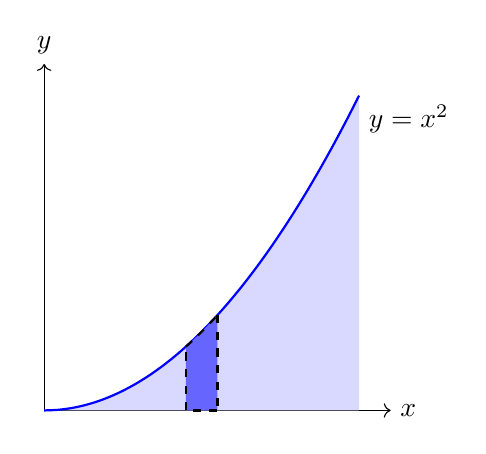
\begin{tikzpicture}[scale=4]
  % Axes
  \draw[->] (0,0) -- (1.1,0) node[right] {\(x\)};
  \draw[->] (0,0) -- (0,1.1) node[above] {\(y\)};

  % Area under full curve (light)
  \begin{scope}
    \clip (0,0) rectangle (1,1.1);
    \fill[blue!15] (0,0) plot[domain=0:1, variable=\x] ({\x}, {\x*\x}) -- (1,0) -- cycle;
  \end{scope}

  % Parabola
  \draw[domain=0:1, smooth, variable=\x, blue, thick] plot ({\x}, {\x*\x});
  \node at (1,1) [below right] {\(y = x^2\)};

  % Area under the curve in small interval [0.45, 0.55]
  \begin{scope}
    \clip (0,0) rectangle (1,1.1);
    \fill[blue!60] 
      (0.45,0)
      -- plot[domain=0.45:0.55, variable=\x] ({\x}, {\x*\x})
      -- (0.55,0) -- cycle;
  \end{scope}

  % Outline of the curved rectangle (complete)
  \draw[thick, dashed] (0.45,0) -- (0.45,{0.45*0.45});
  \draw[thick, dashed, domain=0.45:0.55, variable=\x] plot ({\x}, {\x*\x});
  \draw[thick, dashed] (0.55,{0.55*0.55}) -- (0.55,0);
  \draw[thick, dashed] (0.55,0) -- (0.45,0);
  \draw[thick, dashed] (0.45,0) -- (0.45,{0.45*0.45}); % ← questo è il lato che mancava

\end{tikzpicture}
\end{center}
\\
Abbiamo che su ogni intervallo è possibile costruire un rettangolo più grande e uno più piccolo, in particolare ciò è possibile se la funzione cresce o decresce, nel caso in cui sia costante allora rimaniamo fermi chiaramente.
\\
Sappiamo dunque per certo che la somma dei \virgolette{rettangoli superiori} è $\geqslant$ \virgolette{somma dei rettangoli inferiori}.
\\
Matematicamente, dunque, possiamo scrivere che:
\begin{equation*}
    A_p \geqslant \sum_{k=0}^{n-1}(x_{k+1}-x_k)f(x_k) \,\,\,\,\,\,\, \mbox{dove}\,\,\,\,\,\,\,\,(x_{k+1}-x_k)=\frac{1}{n}\,\,\,\,\,\,, \,\,\,\,\,\,\, f(x_k)=\frac{k^2}{n^2}
\end{equation*}
Facciamo adesso lo stesso ragionamento con i rettangoli superiori:
\begin{equation*}
    A_p \leqslant \sum_{k=0}^{n-1}\frac{1}{n}\frac{(k+1)^2}{n^2}
\end{equation*}
Se mettiamo tutto assieme diventa allora:
\begin{equation*}
 \sum_{k=0}^{n-1}(x_{k+1}-x_k)f(x_k)  \leqslant   A_p \leqslant \sum _{k=0}^{n-1}\frac{1}{n}\frac{(k+1)^2}{n^2}
\end{equation*}

Possiamo però calcolare queste somme, infatti:
\begin{equation*}
    \sum_{k=0}^{n-1}\frac{1}{n}\frac{k^2}{n^2}=\frac{1}{n^3}\sum_{k=0}^{n-1}k^2=\frac{1}{n^3}\frac{(n-1)(n)(2(n-1)+1)}{6} \texttildelow \frac{2n^3}{6n^3}=\frac{1}{3}
\end{equation*}
Facciamo il calcolo analogo con i rettangoli superiori e otteniamo:
\begin{equation*}
    A_p \leqslant  \sum_{k=0}^{n-1} \frac{1}{n}\frac{(k+1)^2}{n^2}=\sum_{k=0}^{n-1} \texttildelow \frac{1}{3}
\end{equation*}
Per lo stesso motivo di prima.
\subsection{Assunzione generale}
In tutto questo capitolo, quando introduciamo una funzione, bisogna pensarla sempre definita nel dominio su un intervallo chiuso e limitato, ossia:
\begin{equation*}
    f: [a,b] \to \R
\end{equation*}
\begin{center}
    \textbf{\textit{Nota}}
\end{center}
La teoria che stiamo per vedere si potrebbe studiare tutta alla stessa maniera senza questa assunzione, ma ciò renderebbe le cose estremamente più complicate e non cambierebbe assolutamente nulla, quindi ci teniamo le cose come sono.
\\
\subsection{Definizioni varie}
\subsubsection{Partizione (di $[a,b]$)}
Una partizione è un sottoinsieme finito e ordinato di $[a,b]$, ossia $\{x_0,x_1,...,x_n\}$ tali che $x_0=a$ e $x_n=b$.
\\
Quando diciamo ordinato stiamo dicendo che $x_k \leqslant x_{k+1} \forall k=0,1,...,n-1$
\subsubsection{Successione di partizioni}
Una successione di partizioni è una funzione $f: \N \owns n \to P_n$ partizione, cioè semplicemente stiamo etichettando delle partizioni
\subsubsection{Raffinamento di partizioni}
Se $P$ è una partizione, $Q$ è un suo raffinamento se $P \subset Q$, cioè che $Q$ contiene i punti di $P$  ne aggiunge altri, in questo senso \virgolette{raffina} $P$
\subsubsection{Somme superiori}
Data $f: [a,b] \to \R$, definiamo come somme superiori di $f$ rispetto a $P$ partizione:
\begin{equation*}
    S(f,P)=\sum_{k=0}^{n-1}(x_{k+1}-x_k)(\underset{[x_k,x_{k+1}]}{sup}(f))
\end{equation*}
\subsubsection{Somme inferiori}
Definiamo come somme inferiori di $f$ rispetto a $P$ partizione:
\begin{equation*}
    s(f,P)=\sum_{k=0}^{n-1}(x_{k+1}-x_k)(inf(f))
\end{equation*}
\subsection{Lemma di disuguaglianze}
Considerando la solita assunzione generale:
\begin{enumerate}
    \item Se $P \subset Q$, con $P$ e $Q$ partizioni, allora:
    \begin{align*}
        s(f,P) \leqslant s(f,Q) \\
        S(f,P) \geqslant S(f,Q)
    \end{align*}
    Cioè in pratica più raffino la partizione più aumento le somme inferiori e diminuisco le somme superiori
    \item Se $m \leqslant f \leqslant M$, allora $\forall P$ partizione si avrà che 
    \begin{equation*}
        m(b-a) \leqslant s(f,P) \leqslant S(f,P) \leqslant M(b-a)
    \end{equation*}
    \item $\forall P,Q$ partizioni, $s(f,P) \leqslant S(f, Q)$
\end{enumerate}
\begin{center}
    \textbf{\textit{Dimostrazione (scritta un pò sbagliata)}}
\end{center}
\begin{enumerate}
    \item $P=\{x_0,...,x_n\}$ e $Q=\{x_0,...,x_n\} \bigcup \{\xi_1,...,\xi_e\}$.
    \\
    Sia poi $\xi=\xi_1 \notin P$ (altrimenti $P=Q$ e 1. è ovvio).
    \\
    Allora $\xi \in (x_k,x_{k+1})$.
    \\
    Adesso vengono i calcoli, infatti:
    \begin{align*}
        s(f,P)=\sum_{\overline{k}=0}^{n-1}(x_{\overline{k}+1}-x_{\overline{k}}) \, \underset{[x_k,x_{k+1}]}{inf} (f)= \\
        \sum_{\overline{k}=0}^{k-1}(x_{\overline{k}+1}-x_{\overline{k}})\underset{[x_k,x_{k+1}]}{inf} (f)+ \sum_{\overline{k}=k-1}^{n-1}(x_{\overline{k}+1}-x_{\overline{k}})\underset{[x_k,x_{k+1}]}{inf} (f)+ \underset{[x_k,x_{k+1}]}{inf} (f) (x_{k+1}- \xi) + \underset{x_k,x_{k+1}}{inf} (\xi - x_k) \\
        \leqslant A+B+ (x_{k+1}-\xi) \underset{[\xi,x_{k+1}]}{inf} (f) + (\xi - x_k)\underset{[x_k,\xi]}{inf (f)}
    \end{align*}

    \vspace{15pt}
    \hrule
    \vspace{15pt}

\subsection{Fatto generale}
Se $U \subset V \subset \R$, allora $inf f ( \mbox{in} \,\,U) \geqslant inf f (\mbox{in} \,\, V)$, infatti, e $x \in U$, allora $x \in V$, dunque $f(x) \geqslant inf (f) (V)$ e dunque $inf (f) (V)$ è minorante dell'insieme $\{f(x) | x \in V\}$ e dunque $inf (f) (V) \leqslant inf (f) (U)$ perchè $inf (f) (U)$ è il più grande dei minoranti

    \vspace{15pt}
    \hrule
    \vspace{15pt}

Concludiamo la dimostrazione di 1. osservando che
\begin{equation*}
    =A+B+ (x_{k+1}-\xi) inf (f) + (\xi - x_k) inf (f) = s(f, P \bigcup \{\xi_1\})=s(f,P \bigcup \{\xi_1,\xi_2\}) \leqslant \underset{\mbox{itero}}{...} \leqslant s(f,Q)
    \cvd
\end{equation*}
\item Se $m \leqslant f \leqslant M$, allora $m \leqslant inf(f) \leqslant supf \leqslant M$.
\\
Bisogna infatti sempre ricordare che il sup è più piccolo dei maggioranti.
\\
Allora abbiamo che $S(f,P)= \sum_{k=0}^{n-1}(x_{k+1}-x_k)\, sup (f) \leqslant \sum_{k=0}^{n-1}(x_{k+1}-x_k) \cdot M= M (b-a)$.
\\
Analogamente $s(f,P) \geqslant m(b-a)$, dunque avremo
\begin{equation*}
    inf (f) (U) \leqslant sup(f)(U) \,\, \Longirghtarrow \,\, S(f,P) \geqslant s(f,P)
\end{equation*}
\item La dimostrazione di 3. segue dalla dimostrazione di 1. perchè, prese singolarmente due partizioni qualunque $P$ e $Q$, pongo $R=P \bigcup Q$, con $R \owns P$ e $R \owns Q$, dunque $s(f,P) \leqslant s(f,R) \leqslant S(f,R) \leqslant S(f,Q)$, dove le disuguaglianze sono state dimostrate, in ordine, dalla 1,2,1.



\end{enumerate}


\subsection{Definizione di una nuova coppia di Dedekind}
Definiamo:
\begin{equation*}
   \R \owns A^-(f)=\{s(f,P) | P \,\,\,\, \mbox{partizione}\}
\end{equation*}
e
\begin{equation*}
   \R \owns A^+(f)=\{S(f,P) | P \,\,\,\, \mbox{partizione}\}
\end{equation*}
Entrambi gli insiemi sono:
\begin{equation*}
    A^\pm (f) \subset [m(b-a), M(b-a)]
\end{equation*}
Insomma, entrambi sono limitati, perchè sono rinchiusi in questo intervallo chiuso e limitato.
\\
Infine sono una \textbf{\textit{coppia di Dedekind}}, dunque, essendo $ \in \R$, $\exixts$ un elemento $\gamma$ chiamato \textit{separatore}.
\begin{center}
    \textbf{\textit{Definizione}}
\end{center}
Sia $f: [a,b] \to \R$ una funzione limitata. Se $(A^-(f),A^+(f))$ ammette un unico elemento separatore, ossia $\gamma \in \R$, allora diremo che $f$ è \underline{Riemann-integrabile}, o \underline{integrabile alla Riemann}, e scriviamo $f \in \mathcal{R} ([a,b])$.
\\
Infine denotiamo $\gamma= \int_a^b f= \int_a^b f(x) dx$, dove ricordiamo che la variabile $x$ dell'ultimo integrale non ha valore, potrebbe essere qualsiasi cosa, per lo meno a questo livello di spiegazione.
\\
\begin{center}
    \textbf{\textit{Osservazioni}}
\end{center}
\begin{itemize}
    \item $\gamma= supA^-(f)=infA^+(f)$ \,\,\,\,\, $\longrightarrow \,\,\,\,\, \mbox{Esiste un UNICO }\,\,\,\,\,\,\,\,\gamma\,\,\,\,\,\,\,\,\,\, t.c. \,\,\,\, a^- \leqslant \gamma \leqslant a^+ $, infatti se per assurdo $\gamma$ non fosse $inf(a^+)$, allora $\exists \,\,\,\,\, \xi \,\,\,\,\,\, t.c. \,\, \gamma < \xi \leqslant a^+$, ma allora $a^- < \xi \leqslant a^+$, ossia esisterebbe un altro elemento separatore, ma è assurdo
    \item Tutte le funzioni del tipo $f(x)=c \forall x \in [a,b]$, ossia tutte le funzioni costanti nell'intervallo $[a,b]$, appartengono a $\mathcal{R}([a,b])$, infatti, se $P$ è una partizione generica, allora $s(f,P)=\sum_{k=0}^{n-1}(x_{k+1}-x_k) inf(f)=\sum_{k=0}^{n-1}(x_{k+1}-x_k) \cdot c = c(b-a)$.
    \\
    Analogamente, $S(f,P)= c(b-a) \,\, \Longrightarrow A^-(f) = \{c(b-a)\}=A^+(f)$.
    \\
    Insomma, $\int_a^b c = c(b-a)$
\end{itemize}
\subsection{Teorema di equivalenza di diverse cose}
Sia $f:[a,b] \to \R$, con $f$ limitata.
\\
Allora sono equivalenti le seguenti affermazioni:
\begin{enumerate}
    \item $f \in \mathcal{R}([a,b])$
    \item Se pongo $\delta(P)=max (x_{k+1}-x_k)$, dove $P=\{x_0,...,x_{n-1}\}$ partizione di $[a,b]$
    \\
    (chiamo $\delta(P)$ il \textbf{passo} della partizione, l'intervallo più grosso tra tutti quelli che ho).
    \\
    Allora abbiamo che $\forall$ successione di partizioni $\{P_n\}$ tali che $\delta(P_n) \to 0$ si ha che $s(f,P_n)$ ammette limite e , $\lim_{n \to +\infty} S(f,P_n)=\lim_{n \to +\infty}s(f,P_n)=\int_a^b f$
    \item $\forall \,\,\, \varepsilon > 0 \,\,\, \exists \,\,\, P=P_\varepsilon$ tale che $0 \leqslant S(f,P_\varepsilon)-s(f,P_\varepsilon) < \varepsilon$
    \item $\forall $ successione di partizioni $\{P_n\}$ tale che $\delta(P_n) \to 0$ e qualunque selezione di punti $\{\xi_1,...,\xi_{N(n)}\}$ tale che $\xi \in (x_i^n, x_{i+1}^n)$ dove $\{x_0^{(n)},...,x_{N(n)}^{(n)}\}$.
    \\
    Si ha dunque che
    \begin{equation}
    \lim_{n \to +\infty} \sum_{k=0}^{N(n)-1}(x_{k+1}^{(n)}-x_k^{(n)}) \,\, \cdot \, f(\xi_k^{(n)})=l \in \R \,\,\,\, e \,\,\,\,\,   l= \int_a^b f 
    \end{equation}
    Stiamo dicendo che, SOLO QUANDO IL PASSO TENDE A 0, ossia $\delta P \to 0$, se io prendo un punto $\xi$ a caso e prendo i rettangoli con altezza $f(\xi_n)$ e li sommo tutti, allora ho calcolato proprio l'integrale della funzione in quel determinato intervallo.
    \begin{center}
        \textbf{\textit{Esercizio}}
    \end{center}
    Fare esempi grafici su ognuna di queste 4 definizioni
\end{enumerate}
\begin{center}
    \textbf{\textit{Domande/Riflessioni}}
\end{center}
\begin{itemize}
    \item Una funzione costante ma con una discontinuità eliminabile in un punto a caso rimane integrabile? Sì, si dimostra spezzando le somme e poi sfruttando il fatto che posso trovare una $P_\varepsilon$ per soddisfare la terza definizione
    \item Dimostrare che se ha due discontinuità eliminabili rimane integrabile comunque (stessa cosa ma con due punti)
    \item Dimostrare che se ho una quantità numerabile di discontinuità allora la funzione rimane sempre integrabile (si itera un numero $n$ finito di volte il processo fatto all'inizio)
\end{itemize}

\subsection{Partizione regolare}
Spesso, per le funizoni Riemann-integrabili, ha senso scegliere una partizione regolare, ossia, presa una funzione del tipo $f:[a,b] \to \R$, definiamo, per $n \in \N$, una partizione del tipo:
\begin{equation*}
    P_n=\{a, a+ \frac{b-a}{n}, a+ 2\frac{b-a}{n},...,a+ \frac{k}{n}(b-a)\}_{k=1,...,n}
\end{equation*}
dove $x_0=a$ e $x_n=b$.
\\
Scegliamo allora $\xi_k=x_k$, cioè il punto sinistro di ogni piccolo intervallo, e, in questo contesto, dire che la funzione è Riemann-integrabile equivale a dire che 
\begin{equation*}
    \lim_{n \to +\infty} \sum_{k=0}^n f(x_k= a+(b-a)\frac{k}{n})(\frac{b-a}{n})=\int_a^b f
\end{equation*}
\subsection{Funzioni Riemann-integrabili e proprietà}
\subsubsection{Controesempio di Dirichlet}
Sia $f:[0,1] \to \R$, con 
\begin{equation*}
    f(x)=\begin{cases}
        1 \,\,\,\, \mbox{se} \,\,\,\, x \in \mathbb{Q} \cap [0,1] \\
        0 \,\,\,\, \mbox{se} \,\,\,\, x \notin \mathbb{Q} \cap [0,1]
    \end{cases}
\end{equation*}
Calcoliamo allora $S(f,P)$ su $P=\{x_0,...,x_n\}$.
\\
$S(f,P)=\sum_{k=0}^{n-1}(x_{k+1}-x_k)sup(f)$, sove $sup(f)$ è il sup in $[x_k,x_{k+1}]=1$, e questo perchè qualsiasi intervallo contiene infiniti razionali, dunque il sup deve essere sempre 1, cioè $\exists \,\,\, q \in \mathbb{Q} \bigcap [x_k,x_{k+1}]$.
\\
    \vspace{15pt}
    \hrule
    \vspace{15pt}

\begin{center}
    \textbf{\textit{Spieghiamo meglio la densità di $\mathbb{Q}$ in $\R$}}
\end{center}
$\mathbb{Q}$ è denso in $\R$ nel senso che $\forall a \in \R, \,\, r > 0, \,\,\, \exists \,\,\, q \in \mathbb{Q} \bigcap (a-r,a+r)$.
\\
Analogamente l'inf della funzione è sempre 0 per lo stesso motivo!
    \vspace{15pt}
    \hrule
    \vspace{15pt}
Dunque sappiamo che $S(f,P)=1$ e $s(f,P)=0$ e dunque $S(f,P)-s(f,P)=1$.
\\
Allora concludiamo dicendo che $\forall P \,\,\, \mbox{partizione} \Longrightarrow f \notin R([a,b])$, ossia $f$ è integrabile nell'intervallo $[a,b]$, questo perchè esistono infiniti elementi separatori tra le somme superiori e le somme inferiori, e per la nostra prima definizione di integrale di Riemann si ha che l'elemento separatore, per potere essere l'integrale, deve essere UNICO
\\
\subsection{Teorema (dimostrazione omessa perchè noiosa)}
Se $f,g \in R([a,b])$, allora:
\\
$f^2; f \cdot g ; f+g ; cf \,\, (c \in \R) ; \left|f\right| $ sono tutte integrabili

\subsection{Teorema proprietà dell'integrale}
Se $f,g \in R([a,b])$, allora:
\begin{enumerate}
    \item (Linearità), ossia $\int_{a}^b f+g=\int_a^b f + \int_a^b g$, e inoltre $\int_a^b cf= c\int_a^b f$
    \item (Confronto e positività), ossia, se $f \geqslant g$, allora $\int_a^b f \geqslant \int_a^b g$, e, in particolare, se $f \geqslant 0$, $\int_a^b f \geqslant 0$
    \item (Disuguaglianza triangolare):
    \begin{equation*}
        \left|\int_a^b f\right| \leqslant \int_a^b\left|f\right|
    \end{equation*}
    \item (Linearità rispetto al dominio di integrazione):
    \\
    Preso $c \in [a,b]$, allora $\int_a^b f= \int_a^c f + \int_c^b f$
\end{enumerate}

\begin{center}
    \textbf{\textit{Dimostrazioni (tutte tranne la 4)}}
\end{center}
\begin{enumerate}
    \item Consideriamo $P_n=\{x_k=a+\frac{b-a}{n}k\}_{k=0,...,n}$ partizione regolare, e considero
    \begin{equation*}
        \sum(f(x_k)+g(x_k)) \, \frac{b-a}{k} = \sum_{k=0}^n f(x_k)\frac{b-a}{n}+\sum_{k=0}^n g(x_k)\frac{b-a}{n}=\int_a^b f + \int_a^b g
    \end{equation*}
    Dunque SE L'INTEGRALE ESISTE è la somma degli integrali.
    \\
    Insomma, il limite delle somme parziali a sinistra esiste ( e dunque vale $\int_a^b f+g$) e vale $\int_a^b f + \int_a^b g$
    \\
    - Analogamente, preso $c \in \R$, $\sum_{k=0}^n cf(x_k)\frac{b-a}{n}=c\sum_{k=0}^n f(x_k)\frac{b-a}{n}=c\int_a^b f$
    \item Sia $f \geqslant g $ e consideriamo la stessa partizione regolare di prima, alora:
    \begin{equation*}
        \sum_{k=0}^n f(x_k)\frac{b-a}{n} \geqslant \sum_{k=0}^n g(x_k)\frac{b-a}{n}
    \end{equation*}
    e dunque
    \begin{equation*}
        \int_a^b f \geqslant \int_a^b g
    \end{equation*}
    E quest'ultima disuguaglianza vale per i TEOREMA DI CONFRONTO DELLE SUCCESSIONI.
        \vspace{15pt}
    \hrule
    \vspace{15pt}
\begin{center}
    \textbf{\textit{Osservazione}}
\end{center}
Se $g=0$ $(g(x)=0 \,\, \forall x \in [a,b])$, allora $\int_a^b g = \lim_{n \to +\infty}\sum_{k=0}^n g(x_k) \frac{b-a}{n} =0$

\begin{center}
    \textbf{\textit{Esercizio (difficile teschio morte)}}
\end{center}
Dimostrare che, se $f \in C^0([0,1])$, ossia continua in $[0,1]$ e $f > 0 \,\, \forall x$, allora $\int_a^b > 0$.
\\
Se poi $f \in R([a,b])$ e $f > 0 \,\,\, \forall x$, allora $\int_a^b f > 0$
\\
[\'E VERO]
    \vspace{15pt}
    \hrule
    \vspace{15pt}
\item Sappiamo che $f \leqslant |f|$ e che $-|f| \leqslant f \leqslant |f|$.
\\
Questo implica che
\begin{equation*}
\int_a^b(-|f|) \leqslant \int_a^b f \leqslant \int_a^b |f|
\end{equation*}
Ma $\int_a^b (-|f|)=-\int_a^b(|f|)$.
\\
Allora $-\int_a^b |f| \leqslant \int_a^b f \leqslant \int_a^b |f| \,\,\, \Longrightarrow |\int_a^b f| \leqslant \int_a^b |f|$
\end{enumerate}
\begin{center}
    \textbf{\textit{Osservazioni}}
\end{center}
L'integrale di Riemann è un primo concetto di area, è però un'area con un segno, un segno convenzionale, dato che abbiamo deciso di prendere $x_{k+1}-x_k$ come base dei rettangoli, con $x_{k+1}-x_k > 0$.
\begin{center}
    \textbf{\textit{Notazione}}
\end{center}
Se inverto tutti gli intervalli faccio $\int_a^b f = -\int_a^b f$, e possiamo giustificarlo con l'osservazione di prima, ossia con il fatto che il segno è convenzionale e dipende dalla base dei rettangolini, se infatti mi muovo al contrario, la base è un numero negativo e dunque l'area è negativa, ma è tutta convenzione.
\\
\begin{center}
    \textbf{\textit{Osservazione}}
\end{center}
Se prendiamo una Riemann-integrabile $f \in R([\alpha,\beta])$ e $a < b < c$, allora avremo 
\begin{equation*}
    \int_a^b f = \int_a^c f- \int_b^c f \,\,\, \Longrightarrow \int_a^b f =\int_a^c f +\int_c^b f
\end{equation*}

\subsection{Teorema delle funzioni integrabili}
$C^0([a,b]) \subset R([a,b])$, cioè le \underline{funzioni continue sono integrabili}.
\\
    \vspace{15pt}
    \hrule
    \vspace{15pt}
\begin{center}
    \textbf{\textit{Richiamo alle funzioni uniformemente continue}}
\end{center}
$f \in UC([a,b])$ se $\forall \varepsilon > 0 \,\,\, \exists \,\, \delta > 0$ tale che $|f(x)-f(y)| < \varepsilon$ e $sup|x-y|< \delta$ (funzioni uniformemente continue).
\begin{center}
\textbf{\textit{Heine-Cantor}}
\end{center}
$C^0([a,b])=UC([a,b])$
\begin{center}
    \textbf{\textit{Dimostrazione}}
\end{center}
Sia $\varepsilon > 0$, cerco $P=P_{\varepsilon}$ partizione tale che $S(f,P)-s(f,P) < \varepsilon$.
\\
Se chiamo $P=\{x_0,...,x_n\}$ allora 
\begin{equation}
    S(f,P)-s(f,P)=\sum_{k=0}^n(sup(f)-inf(f))(x_{k+1}-x_k)=\sum_{k=0}^{n-1}(f(\varepsilon_k^+)-f(\varepsilon_k^-)(x_{k+1}-x_k) \,\,\,\,\,\,\, \mbox{dove}\,\,\,\,\,\,\,\, f(\varepsilon_k^+)=sup(f)\,\,\,\ e \,\,\,\,\,f(\varepsilon_k^-)=inf(f)
\end{equation}, e questo è vero perchè per WEIERSTRASS una funzione continua in $[a,b]$ assume massimo e minimo.
\\
Sia poi $\delta > 0$ tale che, se $|x-y|<\delta$, allora $|f(x)-f(y)|<\frac{\varepsilon}{b-a}$, e ciò è possibile per uniforme continuità.
\\
Scelgo allora $P$ tale che $\delta(P)$ (il passo) è $\delta(P) < \delta$.
\\
Ora, $\varepsilon_k^+, \varepsilon_k^- \in [x_k, x_{k+1}]$ e $|x_{k+1}-x_k| \leqslant \delta(P) < \delta $, mi assicura che se prendo due punti in $[x_k,x_{k+1}]$, allora so che $|\varepsilon_k^+ - \varepsilon_k^-|< \delta$ e, dunque, $|f(\varepsilon_k^+)-f(\varepsilon_k^-)|<\frac{\varepsilon}{b-a}$.
\\
Allora \begin{equation}
    \sum_{k=0}^{n-1}(f(\varepsilon_k^+)-f(\varepsilon_k^-))(x_{k+1}-x_k) \leqslant \sum_{k=0}^{n-1}\frac{\varepsilon}{b-a}(x_{k+1}-x_k)=\frac{\varepsilon}{b-a}(b-a)=\varepsilon
    \end{equation}

\section{Teoria (classica) di integrazione}
\subsection{Teorema della media integrabile, o Teorema della media}
Sia $f:[a,b] \to \R$ una funzione continua. Allora $\,\, \exists \,\, c \in [a,b]$ tale che $f(c)=\frac{1}{b-a}\int_a^b f$.
\\
Cioè possiamo riscriverla come $(b-a)f(c)=\int_a^b f$.
\\
In pratica quello che vogliamo dire è che, se la funzione è continua, ci sarà un punto c tale che il rettangolo con base $b-a$ e altezza $f(c)$ è esattamente uguale all'integrale della funzione nell'intervallo $[a,b]$.
\\
\begin{center}
    \textbf{\textit{Dimostrazione}}
\end{center}
Sia $m=min(f)$ in $[a,b]$.
\\
Sia $M=max(f)$ in $[a,b]$.
\\
\'E noto che $\forall \,\,\, x \in [a,b]$, vale $m \leqslant f \leqslant M$, ma sappiamo che, per il confronto (punto 2 delle proprietà dell'integrale), vale
\begin{equation*}
    \int_a^b m dx \leqslant \int_a^b f(x) \leqslant \int_a^b M dx
\end{equation*}
Il che implica 
\begin{equation*}
    m(b-a) \leqslant \int_a^b f(x) dx \leqslant M(b-a)
\end{equation*}
e dunque
\begin{equation*}
    m \leqslant \frac{1}{b-a}\int_a^b f \leqslant M
\end{equation*}
Per il teorema dei valori intermedi $\exists \,\,\, c \in [a,b]$ tale che $f(c)=\gamma$

\subsection{Teorema fondamentale del calcolo integrale(TFCI)}
Sia $f \in C^0([a,b])$. Sia poi $F(x)=\int_a^x f(t)dt=\int_a^xf$, se $x \in [a,b]$.
\\
Allora $F \in C^1([a,b])$ e vale $F'=f$
\begin{center}
    \textbf{\textit{Dimostrazione}}
\end{center}
Per calcolare la derivata facciamo uso del rapporto incrementale, dunque:
\\
Sia $x \in [a,b)$, sia $x+h \in [a,b]$, allora:
\begin{equation*}
    \frac{F(x+h)-F(x)}{h}=\frac{1}{h}\left(\int_a^{x+h}-\int_a^x f\right)=\frac{1}{h}\left(\int_a^x f- \int_x^{x+h} f + \int_a^{x}f\right)=\frac{1}{h}\int_x^{x+h}f
\end{equation*}
Per il teorema della media $\frac{1}{h}\int_x^{x+h} f =\frac{1}{h}\left((x+h-x) \,\, f(\varepsilon_n)\right)=\frac{1}{h}(h f(\varepsilon_n))=f(\varepsilon_n)$.
\\
Se poi $h \to 0$, allora $\varepsilon_n \to x$, per il teorema dei carabinieri, perchè
\begin{equation*}
    x \leqslant \varepsilon_n \leqslant x+h
\end{equation*}
e dunque, per il teorema ponte, $f(\varepsilon_n) \to f(x)$
\\
\cvd

\subsection{Intermezzo}
Sia $f:[a,b] \to \R$. Chiamo PRIMITIVA di $f$ una funzione $F: [a,b] \to \R$ tale che \underline{$F$ è derivabile} e \underline{$F'=f$}.
\\
\begin{center}
    \textbf{\textit{Esercizio/Osservazione}}
\end{center}
Non tutte le funzioni ammettono primitiva, ad esempio:
\begin{align*}
    f:[-1,1] \to \R  \\
    x \mapsto \begin{cases}
        0, x \in [-1,0] \\
        1, x \in (0,1]
    \end{cases}
\end{align*}
Se $F$ fosse una primitiva, allora, per $x \in [-1,0)$, $F(x)=c_1$, con $c_1 \in \R$.
\\
Se invece $x \in (0,1]$, $F(x)= x + c_2$.
\\
Dunque $F(x)$ risulta discontinua, per cui non è derivabile e dunque non può essere una primitiva.
\\
\subsection{Lemma}
Se $F$ e $G$ sono due primitive di $f:[a,b] \to \R$, allora $F=G+C$, con $c \in \R$, ossia, la primitiva è unica a meno di una costante additiva.
\\
Inoltre, se $F=G+C$, con $c \in \R$, e $F$ è primitiva di $f$, anche $G$ lo è.
\\
\begin{center}
    \textbf{\textit{Dimostrazione}}
\end{center}
Se $F'=f$ e $G=F-c$, se $G'=(F-c)'=F'=f$.
\\
Allora $F'=f=G'$, inoltre $F'-G'=0=(F-G)'$, cioè, per Lagrange $F-G$ è una costante
\subsection{Formula fondamentale del calcolo integrale}
Sia $f \in C^0([a,b])$. Allora $\int_a^b f=F(b)-F(a)$, dove $F$ è una qualunque primitiva.
\begin{center}
    \textbf{\textit{Dimostrazione}}
\end{center}
$F(x)=\int_a^x f$, allora grazie al TFCI, $F$ è una primitiva.
\\
Inoltre, $F(b)-F(a)=\int_a^bf-\int_a^a f=\int_a^b f$.
\\
Se $G$ è un'altra primitiva di $f$, allora, grazie al lemma precedente, $\exists \,\, c \in \R$ tale che $G=F+c$.
\\
Dunque $G(b)-G(a)=F(b)+c-F(a)-c=F(b)-F(a)=\int_a^b$


\subsection{Tecniche per il calcolo degli integrali}
\subsubsection{Integrazione per parti (IPP)}
Ricordiamo innanzitutto che:
\begin{equation*}
    (f \cdot g)'=f'g+fg' \, \Longrightarrow \int (fg)'=\int f'g + \int g' f \, \Longrightarrow \int f'g = \int (fg)' - \int g' f \, \Longrightarrow \int f'g= fg - \int g'f
\end{equation*}
Infatti $\int (fg)'$ è una primitiva di $(fg)'$, ad esempio una primitiva è proprio $f \cdot g$.
\\
Dunque otteniamo la formula per l'integrazione per parti, ossia:
\begin{equation*}
    \int f'g = fg- \int f g'
\end{equation*}
Se invece vogliamo parlare di integrali definiti, allora il discorso diventa uguale ma con gli integrali definiti, cioè otteniamo:
\begin{equation*}
    \int_a^b f'g = [fg]_a^b - \int_a^b fg'
\end{equation*}
Per dimostrarlo si fa lo stesso identico ragionamento, semplicemente con gli integrali definiti, ossia:
\begin{equation*}
    (f \cdot g)'=f'g+fg' \, \Longrightarrow \int_a^b (fg)'=\int_a^b f'g + \int_a^b g' f \, \Longrightarrow \int_a^b f'g = \int_a^b (fg)' - \int_a^b g' f \, \Longrightarrow \int_a^b f'g= fg - \int_a^b g'f
\end{equation*}

\begin{center}
    \textbf{\textit{Osservazione}}
\end{center}
Nel momento in cui dimostriamo con gli integrali definiti, ci accorgiamo che la scelta della primitiva è ininfluente, perchè anche scegliessimo una primitiva con la costante additiva, allora otterremo che l'integrale totale ha una costante additiva, ma come ben sappiamo non è influente ai fini dell'integrale, semplicemente serve a generalizzare e a parlare di una classe di funzioni

\begin{center}
\textit{\textbf{{Esercizi sul calcolo integrale (abbastanza semplici)}}}
\end{center}
\begin{itemize}
    \item $\int x e^x dx$
    \item $\int arctg(x) dx$
    \item $\int ln(x) dx$
    \item $\int sin(x) e^x dx$
\end{itemize}
\subsubsection{Seconda tecnica: cambio di variabile}
Siano $f$ continua e $\vaphi$ derivabile con derivata continua.
\\
Allora l'integrale $\int f(\varphi (x))\varphi ' (x) dx = \int f(y) dy$, con $y=\varphi (x)$.
\\
Questo vale a dire che: \virgolette{Una primitiva $U(x)$ della funzione $f(\varphi(x))\varphi'(x)$ è data da $f \ \varphi$, dove $F$ è una primitiva di $f$}
\begin{center}
    \textbf{\textit{Dimostrazione}}
\end{center}
Se $U$ è primitiva di $f(\varphi(x)) \varphi ' (x)$, allora $U'(x)=f(\varphi(x)) \varphi ' (x)$.
\\
Se $V(x)=(F \circ \varphi)(x)=F(\varphi(x))$, si ha che $V'(x)=F'(\varphi(x)) \varphi'(x)$ e quindi le derivate coincidono, cioè $V=U+c$
\\
Come conseguenza di ha allora che $\int_a^b f(\varphi(x))\varphi ' (x) dx = \int_{\varphi(A)}^{\varphi (B)} f(t) dt$.
\\
Infatti, se, come prima, $U(x)=\int f(\varphi(X))\varphi'(x) dx$, allora
\begin{equation*}
    \int_a^b f(\varphi(x))\varphi'(x) dx= U(b)-U(a)
\end{equation*}
Per la formula fondamentale del calcolo integrale.
\\
Ma $U=F \ \varphi$, per tutto il discorso precedente, dunque
\begin{equation*}
    \int_a^b f(\varphi(x))\varphi'(x) dx = U(b)-U(a)= F(\varphi(b))-F(\varphi(a))=\int_{\varphi(a)}^{\varphi(b)} f(t) dt
\end{equation*}
Perchè $F$ è primitiva di $f$
\begin{center}
    \textbf{\textit{Osservazione (formula)}}
\end{center}
La formula precedente implica che:
\begin{equation*}
    \int_A^B f(x) dx = \int_{\varphi(A)^{-1}}^{\varphi(B)^{-1}} f(\varphi(x))\varphi'(x) dx
\end{equation*}
\begin{center}
    \textbf{\textit{Dimostrazione}}
\end{center}
Scrivo $A=\varphi(a)$ e $B=\varphi(b)$ nella formula generale.
\begin{center}
    \textbf{\textit{NOTA}}
\end{center}
Attenzione perchè in questo caso è necessario che la funzione $\varphi$ sia invertibile 


\begin{center}
    \textbf{\textit{Esercizi semplici}}
\end{center}
\begin{itemize}
    \item $\int \frac{x}{1+x^2}dx$
    \item $\int sin(x) cos(x) dx$ (occhio!)
    \item $\int sin^2(x) dx$ (formula di duplicazione)
    \item $\int cos^4(x) dx$
\end{itemize}

\subsubsection{Trucco per l'integrazione di funzioni che dipendono da seni e coseni}
Quando abbiamo funzioni del genere:
\begin{equation*}
    \int \frac{sin(x)+1}{5+ cos(x)}dx
\end{equation*}
Possiamo avere un cambio di variabile, ossia $t=tg(\frac{x}{2})$, e, in effetti, segue che $dx=\frac{2}{1+t^2}$.
\\
Inoltre si può dimostrare che $sin(x)=\frac{2t}{1+t^2}$ e che $cos(x)=\frac{1-t^2}{1+t^2}$.
\\
A quel punto sostituisci dentro e te la porti come frazione di polinomi, che vedremo più avanti.
\\

\section{Integrali generalizzati(o impropri)}
Finora abbiamo visto $f \in R([a,b])$, e questo richiedeva (tra le altre cose) che il grafico di $f$ fosse un oggetto geometrico limitato in $\R^2$.
\\
L'integrale improprio cerca fondamentalmente di eliminare questa limitazione, sia sul dominio che sul codominio.
\\
\begin{center}
    \textbf{\textit{Esempio}}
\end{center}
Se prendo $f:(0,1] \to \R$ che associa $x \mapsto \frac{1}{\sqrt{x}}$ questa funzione NON è Riemann-integrabile, perchè l'intervallo $(0,1]$ non è un intervallo chiuso e $f$ non è limitata.
\\
Possiamo però comunque chiederci quanto vale l'integrale di questa funzione, magari vale $+\infty$, ma comunque è lecito chiederselo.
\newpage
\begin{center}
    \textbf{\textit{Cosa facciamo quando stiamo svolgendo un integrale improprio}}
\end{center}
Quando facciamo un integrale improprio non stiamo facendo altro che considerare una funzione (che sarebbe di base definita in un intervallo aperto), in un intervallo chiuso, considerando dunque un punto $\alpha$ molto prossimo allo zero, ma tale che possiamo chiudere l'intervallo e rendere Riemann-integrabile la funzione.
\\
Fondamentalmente, considerando l'esempio di prima, consideriamo $f \in R([\alpha,1]) \forall \alpha > 0$, dunque a quel punto ha senso definire
\begin{equation*}
    \int_0^1 f = \lim_{\alpha \to 0^+}\frac{1}{\sqrt{x}}dx
\end{equation*}
Cioè calcoliamo $\int_\alpha^1 f$ e poi facciamo tendere $\alpha$ a 0.
\\
Sempre riguardo l'esempio inoltre, troviamo una forte analogia con la serie $\frac{1}{\sqrt{n}}$, e anch'essa convergeva, questa similitudine sarà formalizzata successivamente con il criterio  serie-integrale.
\begin{center}
    \textbf{\textit{Definizione}}
\end{center}
Sia $f:[a,b) \to \R$ tale che $f \in R([a, \beta]) \forall a \leqslant \beta \leqslant b$.
\\
Allora
\begin{equation*}
    I=\int_a^b f = \lim_{\beta \to b^-}\int_a^\beta f
\end{equation*}
Cioè facciamo tendere $\beta$ a $b$.
\\
Diremo allora che:
\begin{itemize}
    \item $I$ converge se $I \in \R$
    \item $I$ diverge se $I=\pm \infty$
    \item $I$ non è ben definito (o non converge) se il limite NON esiste.
\end{itemize}

    \begin{center}
        \textbf{\textit{Osservazioni}}
    \end{center}
\begin{itemize}
    \item La definizione precedente vale anche se $b=+\infty$
    \item Si costruisce una definizione \underline{completamente analoga} se $f:(a,b] \to \R$ e $f \in R([\alpha, \beta]) \forall a \leqslant \alpha < \beta$
\end{itemize}

\begin{center}
    \textbf{\textit{Definizione}}
\end{center}
Se $f:(a,b) \to \R$, allora $I=\int_a^b f$ converge se $\forall c \in (a,b)$,
\begin{equation*}
    \int_a^cf \,\,\,\,\, e \,\,\,\,\, \int_c^b f \,\,\,\,\,\,\,\,\,\,\,\,\, \mbox{convergono}
\end{equation*}
Altrimenti diremo che $I$ non converge, come ad esempio $\frac{1}{x(x-1)}$ in $(0,1)$.
\\
\begin{center}
    \textbf{\textit{Piccolo esercizio}}
\end{center}
La definizione è completamente equivalente se sostituisco $\forall \, c$ con $\exists \, c$
\begin{center}
  \textbf{\textit{Definizione}}
\end{center}
  Sia $f:[a,b) \bigcup (b,c] \to \R$, allora $\int_a^c f$ converge se $\int_a^b f$ e $\int_a^c f$ convergono

\begin{center}
    \textbf{\textit{Osservazione}}
\end{center}
Se $f$ è dispari in un intervallo chiuso $[a,b]$ e $f \in R([-1,1])$, allora $\int_{-1}^1 f =0$.
\\
Cioè $\int_{-1}^1 \frac{1}{x}$

\begin{center}
    \textbf{\textit{Notazione}}
\end{center}
Se $\int_a^b f $ converge, allora diremo che $f$ è integrabile
\begin{center}
    \textbf{\textit{Esempio fondamentale}}
\end{center}
$f(x)=\frac{1}{x^\alpha}$ in $[1,+\infty)$ e in $(0,1]$.
\\
\begin{itemize}
    \item $\int_1^{+\infty} \frac{1}{x^\alpha} dx$ converge $\Longleftrightarrow \,\, \alpha > 1$
    \item $\int_0^1 \frac{1}{x^\alpha}dx$ converge $\Longleftrightarrow $ \,\, $\alpha < 1$.
\end{itemize}

\subsection{Proposizione}
Sia $f:(a,b] \to \R$ tale che $f$ è continua ($f \in C^0([a,b])$ e $f$ è estendibile per continuità in $\R$ 
\\
Ricordiamo che estendibile per continuità in $\R$ vuol dire che $\exists \,\,\, p =\lim_{x \to a} \,\,\,\, f(x) \in \R$.
\\
Allora, se 
\begin{equation*}
    \overline{f(x)}=\begin{cases}
        f(x) ,\,\,\,\,\, x \in (a,b] \\
        p , \,\,\,\, x=a
    \end{cases}
  
\end{equation*}
vale che $\int_a^b f$ converge e vale $\int_a^bf=\int_a^b \overline{f}$.

\begin{center}
    \textbf{\textit{Dimostrazione}}
\end{center}
Sia $a < \alpha < b$
\\
Consideriamo 
\begin{equation*}
    \left|\int_\alpha^b f- \int_a^b \overline{f}\right|=\left|\int_\alpha^b f - \int_a^\alpha \overline{f}-\int_a^b f\right|=\left|\int_a^\alpha \overline{f}\right| \leqslant max\left|\overline{f}\right|(a-\alpha) \to 0 \,\,\,\,\,\, \mbox{quando} \,\,\,\,\,\, \alpha \to a
\end{equation*}
Occhio che nell'ultima disuguaglianza abbiamo usato la disuguaglianza triangolare, ossia che $|\int f| \leqslant \int |f|$

\begin{center}
    \textbf{\textit{Esempio}}
\end{center}
Ripensando alla proposizione precedente, se consideriamo l'integrale $\int_0^1 \frac{sin(x)}{x}dx$ allora possiamo dire che converge, perchè possiamo espandere la funzione a $x=0^+$, con $\lim_{x \to 0^+}\frac{sin(x)}{x}=1$ per Taylor


\subsection{Funzioni non nulle, $f \geqslant 0$}
\begin{center}
    \textbf{\textit{Lemma}}
\end{center}
Sia $f:[a,b) \to [0,+\infty)$, $b \in \tilde{\R}$.
\\
Allora $\int_a^b f$ converge $\Longleftrightarrow \,\,\,\,\, F(x) = \int_a^x f(t)dt$ è limitata

\begin{center}
    \textbf{\textit{Dimostrazione}}
\end{center}
\begin{itemize}
    \item Se $\int_a^bf$ converge, allora $\lim_{x \to b}F(x) \,\, \in \R$, allora $f$ è limitata
    \item Sia $F$ limitata, osservo che è anche crescente, infatti, preso $y >x$, vale che:
    \begin{equation*}
        F(y)=\int_a^x f+ \int_x^y f=F(x)+\int_x^y f \geqslant F(x)
    \end{equation*}
    Ma allora osservo che $F(x) \to supF$ quando $x \to b$, e osservo anche che $supF \in \R$, dunque $\int_a^b f$ converge
\end{itemize}

\begin{center}
    \Se $f \geqslant 0$, $\int_a^b f$ converge, e lo scriviamo (se vogliamo) come $\int_a^b f < +\infty$
\end{center}

\subsection{Criterio del confronto}
Siano $f,g:[a,b) \to \R$, con $f,g \geqslant 0$.
\\
Se $f(x) \leqslant g(x) \,\,\, \forall x \in [a,b)$, allora, SE $\int_a^b g < +\infty \,\,\,\,\,\,\ \Longrightarrow \,\,\,\,\,\, \int_a^b f < +\infty$

\begin{center}
    \textbf{\textit{Dimostrazione}}
\end{center}
$F(x)=\int_a^x f$, $G(x)=\int_a^x g$, allora $G(x) \leqslant c$, $\,\,\, \exists c > 0 \,\,\,\,\,\, (\forall x \in \R)\,\,\,\,\,\,\,\,\,\,\, \Longrightarrow F(x)=\int_a^x f \leqslant \int_a^x g \leqslant c \,\,\,\,\,\,\,\ \Longrightarrow \int_a^b f < +\infty$
\\
Fondamentalmente abbiamo sfruttato il lemma precedente con l'ipotesi che $\int_a^b g$ converge, dunque abbiamo detto che $G(x)$ è limitata PER IL LEMMA PRECEDENTE. Poi sappiamo che, per la proprietà degli integrali, vale la disuguaglianza $\int_a^x f \leqslant \int_a^x g$, che in particolare funziona perchè prendo $x in [a,b)$, dunque sto comunque considerando intervalli chiusi, dunque integrali propri, e abbiamo dimostrato che funziona con gli integrali propri.
\\
Dopo di che so che $F(X) \leqslant c$, cioè dunque che $F(x)$ è limitata, e allora, per il lemma precedente $\int_a^b f$ converge.
\\
\subsection{Criterio del confronto asintotico}
Siano $f,g :[a,b) \to [0,+\infty)$, ($f,y \geqslant 0)$ (assumiamole Riemann-integrabili):
\begin{itemize}
    \item Se $f=o(g)$ per $x \to b$ e $\int_a^bg < +\infty$, allora $\int_a^b f < +\infty$
    \item Se $f \texttildelow g$, allora vale $\int_a^b f < +\infty \,\,\,\,\,\, \Longleftrightarrow \,\,\,\,\,\, \int_a^b g < +\infty$
    \item Se $f=O(g)$, se $\int_a^b g < +\infty$, anche $\int_a^b f <+\infty$
\end{itemize}
\begin{center}
    \textbf{\textit{Dimostrazione}}
\end{center}
\begin{center}
    \textbf{\textit{3}}
\end{center}
Se $f=O(g)$ per $x \to b$ vuol dire che $\exists \,\,\,\,\,\,\,\,\ k > 0$, $\exists \,\,\,\,\,\,\, a \leqslant \overline{x} < b \,\,\,\,\,\,\,\,$ tale che $\,\,\,\,\,\,\,\,\,|f(x)| \leqslant k|g(x)| \,\,\,\,\,\,\, \forall \,\,\, x \geqslant \overline{x}$.
\\
Allora posso scrivere $f(x) \leqslant kg(x)$, ma allora, se $F(X)=\int_a^x f(t)dt$:
\begin{itemize}
    \item $\int_a^x f \leqslant \int_a^{\overline{x}} f$ se $x < \overline{x}$
    \item Se invece $x > \overline{x}$, allora 
    \begin{equation*}
        F(x) = \int_a^{\overline{x}}f+\int_{\overline{x}}^xf \leqslant c + \int_{\overline{x}}^x kg(t)dt
        \end{equation*}
        e dunque
        \begin{equation*}
            c+\int_{\overline{x}}^x kg(t)d \leqslant c+kG(x) \leqslant c+kc_1
        \end{equation*}
        Nelle ultime disuguaglianze abbiamo usato, in ordine, il fatto che $\overline{x},x$ è un sottointervallo e dunque l'integrale vale meno che l'integrale di $g$ tra $a$ ed $x$, e poi per ipotesi, per il lemma famoso, sappiamo che $\int_a^x g$ converge, e dunque che $G(x) \leqslant c_1$, per cui arriviamo a dire che $F(x)$ è limitata e dunque, per il lemma precedente, che $\int_a^x f$ converge
\end{itemize}

\begin{center}
    \textbf{\textit{1}}
\end{center}
Vogliamo dimostrare che se $f=o(g)$, allora $f=O(g)$.
\\
Per definizione, se $f=o(g)$, allora $\exists \,\,\,\, \overline{x} \in [a,b)$ tale che $\forall x > \overline{x}$, $|f(x)| < \varepsilon|g(x)|$.
\\
Dunque fissato un $\varepsilon$, torniamo proprio alla definizione di o-grande, e dunque un o-piccolo è un caso specifico di o-grande.

\begin{center}
    \textbf{\textit{2}}
\end{center}
Se $f \texttildelow g$ o $g \texttildelow f$, allora osserviamo che $\frac{f(x)}{g(x)} \to 1$ per $ x \to b$.
\\
Dunque, per definizione di limite, sappiamo che $\forall \varepsilon > 0 \,\,\,\,\,\ \exists \overline{x} \in [a,b)$ tale che $\forall x > \overline{x}$, $|\frac{f(x)}{g(x)}-1|<\varepsilon$.
\\
Dunque $\frac{f(x)}{g(x)}< 1+ \varepsilon$, e dunque, dato $g(x) > 0$ per ipotesi, allora $f(x) < (1-\varepsilon) g(x)$, e dunque, per definizione, $f=O(g)$


\subsection{Criterio serie-integrale}
Sia $f: [1,+\infty) \to [0,+\infty)$ con $f \geqslant 0$ tale che $f$ è decrescente.
\\
Allora $\int_1^{+\infty}f$ converge $\Longleftrightarrow  \,\,\,\,\, \sum_{n \in \N}f(n) < +\infty$
\begin{center}
    \textbf{\textit{Idea grafica (senza disegno)}}
\end{center}
L'idea grafica è che l'integrale tra un naturale e l'altro è perfettamente compreso tra il rettangolino del naturale precedente e quello del naturale successivo, dunque l'area si troverà in mezzo, dunque, se la serie converge, anche l'integrale deve convergere per il criterio del confronto.
\begin{center}
    \textbf{\textit{Dimostrazione}}
\end{center}
$S_n=f(1)+f(2)+...+f(n)$ e $F(x)=\int_1^xf(t)dt$, con $x \in \N$, con $x=n$.
\\
Allora $F(n)=\sum_{k=1}^{n-1}\int_k^{k+1}f$.
\\
Osservo poi che 
\begin{equation*}
    f(k+1) \leqslant \int_{k}^{k+1}f(t)dt \leqslant f(k)
\end{equation*}
Perchè chiaramente $f$ decresce.
\\
In generale allora
\begin{equation*}
    \sum_{k=1}^{n-1}f(k+1) \leqslant F(n) \leqslant \sum_{k=1}^{n-1}f(k)
\end{equation*}
Se poi $\int_1^{+\infty} f < +\infty$, allora $F \leqslant c$, dunque possiamo considerare la successione:
\begin{equation*}
    S_n=\sum_{k=1}^n f(k)=\sum_{k=1}^{n-1}f(k+1)+f(1) \leqslant f(1)+F(n) \leqslant c+f(1)
\end{equation*}
Concludiamo che $\sum f(n) < +\infty$
\vspace{15pt}
\hrule
\vspace{15pt}
Similmente, se $\sum f(n) < +\infty$, allora $S_n \leqslant \overline{c}$.
\\
Ma allora, se $x \in [1,+\infty)$, sia $n \in \N$, $n \geqslant x$, e si ha che
\begin{equation*}
    F(x) \leqslant F(n) \,\,\,\,\,\,\,\,\,\,\,\,\, \mbox{perchè F è crescente}
\end{equation*}
Dunque $F(x) \leqslant F(n) \leqslant S_{n-1} \leqslant \overline{c}$
\cvd
\vspace{15pt}
\hrule
\vspace{15pt}
\begin{center}
    \textbf{\textit{Esercizio}}
\end{center}
$\sum \frac{1}{n^\alpha} < +\infty \,\,\,\,\,\, \Longleftrightarrow \,\,\,\,\,\,\, \alpha > 1$ è dato dal fatto che $\int_1^{+\infty}\frac{1}{x^\alpha}<+\infty \,\,\,\,\,\,\,\,\, \Longleftrightarrow \,\,\,\,\,\,\,\, \alpha > 1$
\begin{center}
    \textbf{\textit{Osservazione}}
\end{center}
Per le serie si ha che $\sum a_n \in \R \Longrightarrow \,\,\, a_n \to 0$, per gli integrali possiamo dire lo stesso???
\\
Cioè, supponiamo che $\int_1^{+\infty}f \in \R$, allora possiamo affermare con certezza che $f \to 0$???




\subsubsection{Lemma (criterio necessario di convergenza)}
Se $\int_1^{+\infty}f \in \R$ e $f(x) \to l \in \R$, allora $l=0$

\begin{center}
    \textbf{\textit{Dimostrazione (esercizio)}}
\end{center}
L'idea è quella di scegliere un tubo all'interno del quale la funzione rimane definitivamente e dire che quindi non converge perchè se integro qualsiasi valore lì dentro allora l'integrale diverge facendo il limite all'infinito.

\begin{center}
    \textbf{\textit{In generale però, questa cosa è falsa}}
\end{center}
Esiste un controesempio per cui $\int_1^{+\infty}f \in \R$ ma $f(x) \nrightarrow 0$.
\\
La funzione è:
\begin{equation*}
    f(x)=\begin{cases}
        1, \,\,\,\,\,\,\,\, x \in [k-\frac{1}{2^{k+1}},k+\frac{1}{2^{k+1}}] \\
        0 \,\,\,\,\,\,\,\, x \notin [k-\frac{1}{2^{k+1}},k+\frac{1}{2^{k+1}}]
    \end{cases}
\end{equation*}
Dunque $\int_1^{+\infty}=\sum \frac{1}{2^k} \in \R$ ma $f \nrightarrow 0$, infatti $f(k) \to 1$


\subsection{Funzioni di segno generico}
Tutto quello che abbiamo visto fino ad ora, parallelamente a quanto fatto per le serie, vale SOLO ED ESCLUSIVAMENTE per le funzioni NON NULLE, vale a dire $f \geqslant 0$.
\\
Analizziamo adesso i criteri che possono tornare utili nello studio della convergenza di integrali impropri nel caso in cui la funzione cambi di segno.
\\
\subsubsection{Criterio di convergenza assoluta (per gli integrali impropri)}
Se \begin{equation*}
    \int_a^b |f| < +\infty
\end{equation*}
Allora 
\begin{equation*}
    \int_a^b f \in \R
\end{equation*}
\begin{center}
    \textbf{\textit{Dimostrazione}}
\end{center}
Definisco $g=|f|-f$ e poi ridefinisco $ f=|f|+(f-|f|)=|f|-g$.
\\
Ora, $g= |f|-f$, ma $0 \leqslant g \leqslant 2|f|$, perchè $\pm f \leqslant |f|$.
\\
Infine osserviamo che $2|f|$ è integrabile perchè
\begin{equation*}
    \int_a^x 2 |f|=2\int_a^x |f| \to 2 \int_a^b |f|
\end{equation*}
e dunque $g$ ha integrale convergente, cioè $\int_a^b g \in \R$.
\\
Dunque osserviamo che $f= |f|- g$ dove $|f|$ è convergente per ipotesi, $g$ è convergente per il criterio del confronto, e dunque somma di integrali convergenti dà un integrale convergente per l'algebra dei limiti, allora diremo che $\int_a^b f \in \R$, cioè che l'integrale di $f$ converge.
\\
\subsubsection{Integrale $\int_{-\infty}^{+\infty} e^{-x^2}$, studio della convergenza}
Chiamiamo $I=\int_{-\infty}^{+\infty} e^{-x^2}$.
\\
Definiamo poi:
\begin{align*}
    I_+=\int_0^{+\infty} e^{-x^2}dx \\
    I_-=\int_{-\infty}^0 e^{-x^2}dx
\end{align*}
Consideriamo $I_+$: se $x \geqslant 1$, allora $e^{-x^2} < e^{-x}$, per cui, siccome sappiamo che $\int_1^{+\infty}e^{-x}dx < +\infty$ perchè sappiamo calcolarlo, allora per il criterio del confronto $I_+$ converge.
\\
Stessa cosa al negativo, dunque $I$ è somma di $I_+$ e $I_-$, elementi che convergono entrambi, e dunque converge anche $I$.
\subsection{Alcuni esempi di funzioni con segno ignoto nell'integrale generalizzato}
\begin{enumerate}
    \item Consideriamo $\int_1^{+\infty} \frac{sinx}{x^2}dx$, applichiamo allora il criterio di convergenza assoluta.
    \\
    $|f(x)|=\frac{|sinx|}{x^2}\leqslant \frac{1}{x^2}$ e dunque $\int_1^{+\infty}\frac{1}{x^2}dx < +\infty$ perchè sappiamo calcolarlo. Dunque l'integrale di partenza converge per il criterio di convergenza assoluta, a cui è seguito il criterio del confronto (cioè prima abbiamo visto che la funzione con il valore assoluta convergeva applicando il criterio del confronto, e quindi abbiamo potuto dire che convergeva anche l'integrale di partenza).
    \\
    \item \textbf{\textit{Esercizio teorico}} \\
    $f(x)=\frac{sinx}{x}$, studiare la convergenza dell'integrale $\int_1^{+\infty}\frac{sinx}{x}$.
    \\
    Possiamo risolvere il problema integrando per parti, ossia:
    \begin{equation*}
        \int_1^{T}\frac{sinx}{x}dx=\left[-\frac{cosx}{x}\right]_1^T \,\,- \int \frac{cosx}{x^2}
    \end{equation*}
    A questo punto l'integrale che ci rimane sappiamo che converge per il primo esempio che abbiamo fatto (era con il seno ma con il coseno è esattamente uguale), dunque risulta che l'integrale $\int_1^{+\infty}\frac{sinx}{x}dx$ è somma di due elementi che convergono, perciò converge anche lui.
    \item Studiamo adesso la convergenza o divergenza dell'integrale $\int_1^{+\infty}\frac{sin^2x}{x}dx$, così da poter dire che anche $\int_1^{+\infty}\frac{sinx}{x}$ diverge, per il criterio del confronto. Per osservare che il primo integrale diverge basta linearizzare il coseno con la formula di duplicazione e osservare che, per l'algebra dei limiti, l'integrale deve divergere. Per il criterio del confronto allora vedremo che anche il secondo integrale deve divergere, al contrario di quanto ci si potrebbe aspettare (perchè la stessa funzione senza il valore assoluto convergeva)
    \item Analizziamo adesso l'integrale $\int_0^{+\infty}\frac{|\sin x|}{x}$, per cui:
    \begin{equation}
        a_n=\int_1^{2\pi n}\frac{|\sin x|}{x}dx \geqslant \int_{2\pi}^{2 \pi n}\frac{|\sin x|}{x}dx=\sum_{k=1}^n \int_{2k\pi}^{2\pi(k+1)}\frac{|\sin x|}{x}dx \geqslant \sum_{k=1}^n \frac{1}{2(k+1) \pi} \int_{2k\pi}^{2\pi (k+1)} |\sin x|dx= \sum_{k+1}^n \left(\frac{c}{2\pi}\right)\frac{1}{k} \underset{n \to +\infty}{ \to +\infty}
    \end{equation}
\end{enumerate}
\subsection{Criterio di Abel}
Siano $f,g : [1,+\infty) \to \R$ funzioni tali che:
\begin{enumerate}
    \item $f \searrow 0$ per $x \to +\infty$
    \item $G(x)=\int_1^x g(t)dt$ è limitata, cioè $|sup(G(x))| < +\infty$.
\end{enumerate}
Allora, SE $f \in C^1([1,+\infty))$ (cioè se la funzione è derivabile con continuità della sua derivata),  $\int_1^{+\infty}fg$ converge.
\begin{center}
    \textbf{\textit{Esempi rapidi e osservazioni}}
\end{center}
\begin{itemize}
    \item $f \in C^1([1,+\infty))$ è un'ipotesi che si può rilassare (cioè è un pò più forte del dovuto)
    \item Il criterio funziona ugualmente se $f,g: [a,b) \to \R$
    \item $\int_1^{+\infty}\frac{sinx cos(9x)}{x}dx$, $G(T)=\int_1^T sinx cos(9x) dx$ si può dimostrare che è una funzione limitata, e dunque l'integrale è convergente proprio perchè prodotto di una $G(x)$ limitata per una decrescente a 0 (che in questo caso sarebbe$\frac{1}{x}$)
\end{itemize}
\begin{center}
    \textbf{\textit{Dimostrazione}}
\end{center}
Sia $U(T)=\int_1^T f(x)g(x)dx$ e vogliamo dimostrare che questo integrale converge.
\\
Cominciamo allora integrando per parti, ossia:
\begin{equation*}
    \int_1^T f(x)g(x)dx= \left[G(x)f(x)\right]_1^T-\int_1^T G(x)f'(x)dx.
\end{equation*}
Chiamiamo allora $G(x)f(x)=V_1(x)$ e $G(x)f'(x)=V_2(x)$.
\\
Adesso, $V_1(x)$ calcolata tra 1 e T ci dà:
\begin{equation*}
    G(T)f(T)-G(1)f(1) \to 0+G(1)f(1)
\end{equation*}
Osserviamo adesso i due pezzi separatamente:
\begin{itemize}
\item E questo perchè $f(T)$ per $T \to +\infty$ tende a 0 per ipotesi, dunque, essendo $G(x)$ limitata, prodotto di limitata per infinitesima tende a 0. Così rimane $G(1)f(1)$ che, essendo l'1 incluso nel dominio (cioè $G(1), f(1) \in \R$), allora è un numero reale, e quindi il primo pezzo converge, andiamo al secondo.
\item A questo punto l'integrale iniziale converge se e solo se converge il secondo integrale arrivato dall'integrazione per parti.
\end{itemize}

\\
Allora, per vedere cosa fa questo integale proviamo ad applicare il criterio di convergenza assoluta, e osserviamo che:
\begin{equation*}
    \int_1^T |Gf'|=\int_1^T |G|(-f')
\end{equation*}
Questo perchè, essendo $f$ una funzione decrescente, allora la sua derivata è negativa e, nel momento in cui applico il valore assoluto, devo mettere di regola un meno davanti.
\\
Dunque abbiamo:
\begin{equation*}
    \int_1^T |G(x)|(-f'(x)) \leqslant |supG(x)|\int_1^T -f'(x) dx= |supG(x)| (f(T)-f(1)) \to c \cdot f(1)
\end{equation*}
Dunque abbiamo dimostrato che l'integrale è maggiorato da un altro integrale che converge, dunque per il criterio del confronto, anche l'integrale di partenza deve convergere. \\
\cvd

\subsubsection{Step linea guida per studiare la convergenza di integrali a caso}
\begin{center}
    \textbf{\textit{Esempio esplicativo}}
\end{center}
$\int_0^{+\infty}\frac{sinx}{x(1-x)}dx$, studiamo la convergenza.
\begin{enumerate}
    \item Bisogna innanzitutto intuire dov'è improprio l'integrale, in questo caso in diversi punti, in particolare $x=0,1, x \to +\infty$
    \item La funzione integranda non ha segno costante (osservare il segno della funzione integranda, definendo intervalli dove ha segno costante)
    \item Consideriamo 4 integrali:
    \begin{equation*}
        I_1=\int_0^\frac{1}{2}f \,\,\,\,\,\,\,\,\,\,\,\,\,\, I_2=\int_{\frac{1}{2}}^1 f \,\,\,\,\,\,\,\,\,\,\,\,\,\, I_3=\int_1^{\frac{3}{2}}f \,\,\,\,\,\,\,\,\,\,\,\,\,\,\, I_4= \int_{\frac{3}{2}}^{+\infty}f
    \end{equation*}
    Quando spezziamo l'integrale facciamolo in modo da spezzarlo nei punti peggiori, così che se un integrale per caso diverge, allora l'esercizio è finito, diverge tutto l'integrale che stiamo studiando.
    In questo caso si osserva che gli integrali addosso a $x=1$ divergono, dunque basta calcolarne uno per concludere l'esercizio e affermare che l'integrale di partenza diverge.
\end{enumerate}
\newpage
\section{Successioni di funzioni}
\subsection{Definizione di successioni di funzioni}
Una successione di funzioni è una funzione
\begin{align}
    F: \N \to X \\
    n \mapsto F(n)
\end{align}
Dove $X$ è uno spazio di funzioni, prenderemo sempre funzioni con dominio nello stesso insieme:
\begin{equation}
    X=\{f: I \to \R \,\, | \,\, I \subset \R\}
\end{equation}
Indicheremo tale successione con $\{f_n\}$
\subsection{Alcuni esempi (importanti)}
\begin{align}
    f_n: [0,1] \to \R \\
    x \mapsto x^n
\end{align}
\begin{center}
    \textbf{\textit{Osservazione}}
\end{center}
Cosa succede se mando $n \to +\infty$??
\\
Se definisco $f(x)=\lim_{n \to +\infty} f_n(x)$, avremo allora:
\begin{equation}
    f(x)=\begin{cases}
        1, \,\,\,\,\, x=1 \\
        0, \,\,\,\,\, x \neq 1
    \end{cases}
\end{equation}
\subsubsection{Definizione di \textbf{tendere puntualmente}}
Sia data 
\begin{equation}
    f_n: I \to \R
\end{equation}
una successione di funzioni.
\\
Diremo allora che $f_n$ \textbf{tende puntualmente} a $f: I \to \R$ se \begin{equation}
    f(x)=\lim_{n \to +\infty}f_n(x) \,\,\, \forall x \in I
\end{equation}
\begin{center}
    \textbf{\textit{Osservazione}}
\end{center}
Osservo che la convergenza puntuale NON mantiene la continuità.
\vspace{15 pt}
\hrule
\vspace{15 pt}
\begin{center}
    \textbf{\textit{Esempio 2}}
\end{center}
Mi chiedo:\\
Se $f_n \to f$ puntualmente (ossia $f_n(x) \to f(x) \,\, \forall \,\, x \in I$, è vero che
\begin{equation}
    \int_a^b f_n \to \int_a^b f \,\,\, ????
\end{equation}
La risposta è NO.
\begin{center}
    \textbf{\textit{Controesempio}}
\end{center}
Riusciamo infatti a trovare un controesempio che contraddice la domanda, infatti consideriamo:
\begin{center}
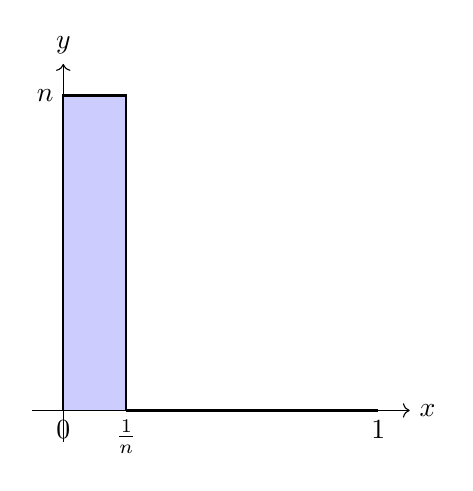
\begin{tikzpicture}[scale=4]

  % Definizione base del rettangolo
  \def\a{0.2} % cioè 1/n

  % Assi
  \draw[->] (-0.1,0) -- (1.1,0) node[right] {$x$};
  \draw[->] (0,-0.1) -- (0,1.1) node[above] {$y$};

  % Etichette
  \node[left] at (0,1) {$n$};
  \node[below] at (0,0) {$0$};
  \node[below] at (\a,0) {$\frac{1}{n}$};
  \node[below] at (1,0) {$1$};

  % Rettangolo azzurro chiaro
  \fill[blue!20] (0,0) rectangle (\a,1);

  % Contorno del rettangolo
  \draw[thick] (0,0) -- (0,1) -- (\a,1) -- (\a,0);

  % Segmento continuo sull'asse x da 1/n a 1
  \draw[thick] (\a,0) -- (1,0);

\end{tikzpicture}
\end{center}
\begin{equation}
    f_n(x)=\begin{cases}
        0, \,\,\,\, x \notin (0, \frac{1}{n}] \\
        n, \,\,\,\, x \in (0, \frac{1}{n}]
    \end{cases}
\end{equation}
Dunque $f_n \to 0$ \underline{puntualmente}, ma
\begin{equation}
    \int_0^1 0 = 0 \neq 1=\int_0^1 f_n
\end{equation}
Dunque abbiamo trovato il controesempio.

\vspace{15 pt}
\hrule
\vspace{15 pt}
\begin{center}
    \textbf{\textit{Esempio 3}}
\end{center}
Sia $f:[0,1] \to \R$, con $f_n \in C^1([0,1])$ e $f_n \to f$ \underline{puntualmente}.
\\
\'E vero che $f \in C^1([0,1])$??? O anche $f'_n \to f'$ ????
\\
Consideriamo \begin{equation}
    f_n(x)=\frac{1}{n}sin(nx)
\end{equation}, allora $f_n(x) \to 0=f(x)$.
\\
Ma $f'_n(x)= cos(nx)$ non tende a nulla

\subsubsection{Definizione di convergere uniformemente}
Sia $f_n: I \to \R$ (con $I \subset \R$) una successione di funzioni.
\\
Diremo che $f_n$ \textbf{converge uniformemente} a $f$ SE:
\begin{equation}
    \forall \,\, \varepsilon > 0 \,\, \exists \,\, N > 0 \,\,\, \text{tale che, se $n > N$}, |f_n(x) - f(x)| < \varepsilon, \,\,\,\, \forall x \in I
\end{equation}
\begin{center}
    oppure
\end{center}
\begin{equation}
    \forall \,\, \varepsilon > 0 \,\, \exists N > 0 \,\,\,\, \text{tale che, se $n > N$}, sup(x \in I)|f_n(x)-f(x)| < \varepsilon
\end{equation}
\begin{center}
    oppure
\end{center}
\begin{equation}
   \underset{x \in I}{sup}\left|f_n - f\right| \to 0 
\end{equation}
\begin{center}
    \textbf{\textit{Esercizio}}
\end{center}
Le due definizioni sono equivalenti, dimostralo (2 $\Longrightarrow$ 1 è facile)
\subsubsection{Notazione}
Data una funzione $g: I \to \R$, $||g||_\infty=sup(g)$, con $x \in I$
\subsubsection{Notazione 2}
Se $f_n$ converge uniformemente a $f$ in $I$, scrivo $f_n \rightrightarrows f $, allora:
\begin{equation}
    f_n \to f \,\,\, (\mbox{se il} \,\, sup \to 0\,\,\, \mbox{allora}\,\,\, f_n-f \to 0, \,\,\, \mbox{a maggior ragione})
\end{equation}
NON \'E VERO IL VICEVERSA!!!!
\begin{center}
    \textbf{\textit{Controesempio}}
\end{center}
Sia 
\begin{equation}
    f_n(x)=\begin{cases}
        x^n \,\,\,\, x \in \left[0,1\right] \\
        0 \,\,\,\, x=1
    \end{cases}
\end{equation}
\'E facile vedere che $f_n \to f$ dove $f(x)=0 \,\,\,\, \forall x \in \left[0,1\right]$.
\\
Ma $f_n$ tende uniformemente a qualcosa? ($f_n \rightrightarrows g$ ??).
\begin{itemize}
    \item Domanda: Se questa ipotesi fosse vera, che funzione sarebbe la funzione $g$?? $g$ deve essere PER FORZA $f$, dunque $g=f$ (dove $f$ è il \textit{limite puntuale}), infatti se $f_n \rightrightarrows g$, allora $f_n \to g$.
    \\
    Ma allora, dato che $f_n \to f, f=g$
\end{itemize}
\begin{center}
    \textbf{\textit{Tirando le somme:}}
\end{center}
Tirando le somme capiamo che se $u_n \to u$, allora $u_n$ può convergere uniformemente \underline{solo} ad $u$
\begin{center}
    \textbf{\textit{Tornando all'esercizio}}
\end{center}
Voglio vedere se $f_n \rightrightarrows 0$, ossia se 
\begin{equation}
    sup|f_n(x) - 0| =supf_n(x)= 1 \nrightarrow 0
\end{equation}
Dunque $f_n$ NON ammette limite uniforme, ossia:
\begin{equation}
    f_n \to f \nRightarrow f_n \rightrightarrows f
\end{equation}

\subsubsection{Teorema di manutenzione della continuità}
Questo teorema dimostra che la \underline{convergenza uniforme} mantiene la continuità.
\\
Sia $f_n: [a,b] \to \R$, con $f_n \in C^0 ([a,b])$.
\\
Se $f_n \rightrightarrows f (: [a,b] \to \R)$ allora $f$ è continua ($f \in C^0([a,b])$)
\begin{center}
    \textbf{\textit{Dimostrazione}}
\end{center}
Dimostriamo che $f$ è continua in un punto a caso per dimostrare che è continua in ogni punto.
\\
Sia $x \in [a,b]$. Mostriamo che, se $y \to x$, allora $f(y) \to f(x)$, da cui $|f(y)-f(x)| \to 0$.
\begin{equation}
    |f(y)-f(x)|=|f(y)-f_n(y)+f_n(y)-f_n(x)+f_n(x)-f(x)| \leqslant |f(y) - f_n(y)| + |f_n(x) - f(x)| + |f_n(y)-f_n(x)| \leqslant 2||f-f_n||_\infty + |f_n(y)-f_n(x)|
\end{equation}
Dove $2||f-f_n||_\infty$ è un NUMERO che dipende solo da $n$ e non da x, posso chiamarlo come voglio, lo chiamo in questo caso $a_n$.
\\
Ora, se $y \to x$, allora $|f_n(y)-f_n(x)| \to 0$ e, per $n \to +\infty$, $a_n \to 0$.
\\
Insomma, $|f(x)-f(y)| \leqslant a_n + o(1) (\mbox{quando} \,\,\, y \to x)$

\subsubsection{Teorema degli integrali sotto convergenza uniforme }
Sia $f_n \subset \mathcal{R}([a,b])$ e supponiamo $f_n \rightrightarrows f$.
\\
Allora \begin{equation}
    \int_a^b f_n \to \int_a^b f
\end{equation}
\begin{center}
    \textbf{\textit{Dimostrazione}}
\end{center}
\begin{equation}
    \int_a^b f_n \to \int_a^b f \,\,\,\, \Longleftrightarrow \,\,\,\, |\int_a^b f_n - \int_a^b f| \to 0
\end{equation}
Questo vale poiché
\begin{equation}
    \left|\int_a^b f_n -\int_a^b f\right| =\left| \int_a^b f_n-f  \right| \leqslant \int_a^b \left|f_n-f\right| \leqslant \int_a^b \left\|f_n-f\right\|_\infty=\left\|f_n-f\right\|_\infty (b-a) \to 0 \,\,\,\,\ \mbox{per convergenza uniforme}
\end{equation}
Adesso, il termine $\left\|f_n-f\right\|_\infty$ è un \textbf{numero}!! Ed è per questo che lo integro come si integra una costante
\begin{center}
    \textbf{\textit{Osservazione}}
\end{center}
Se $f_n \in C^0([a,b]) \subset \mathcal{R}([a,b])$ allora l'enunciato precedente è totalmente corretto (e anche la dimostrazione). Altrimenti dovevamo dimostrare che $f_n \in \mathcal{R}([a,b])$ e che $f_n \rightrightarrows f$, allora $f \in \mathcal{R}([a,b])$. Questo comunque è vero, ma è molto noioso da dimostrare.

\subsubsection{Teorema della derivata (nome mio)}
Sia $\{f_n\}$ una successione di funzioni, $f_n: [a,b] \to \R$, $f_n \in C^1([a,b])$.
\\
Se allora:
\begin{itemize}
    \item $f'_n \rightrightarrows g$
    \item $\exists l \in \R, \,\,\, \exists x_0 \in [a,b]$ tale che $f_n(x_0) \to l$.
    \\
    Allora $\exists f:[a,b] \to \R$, con $f \in C^1([a,b])$ tale che $f(x_0)=l$ e $f_n \rightrightarrows f$ e $f'=g$
\end{itemize}
\begin{center}
    \textbf{\textit{Dimostrazione}}
\end{center}
\begin{center}
    Costruzione di $f$
\end{center}
So che 
\begin{equation}
    f_n(x) = f_n(x_0)+\int_{x_0}^x f_n'(t)dt \to l + \int_{x_0}^x g(t)dt \,\,\,\,\, \mbox{per il teorema precedente}
\end{equation}
Questo mi dice a posteriori che, se chiamo $f(x)=l+\int_{x_0}^x g(t)dt$, ho che
\begin{equation}
    f_n(x) \to f(x)
\end{equation}
Inoltre $f(x_0)=l+\int_{x_0}^{x_0}g=l$.
\\
Da adesso chiamiamo $f(x)=f(x_0)+\int_{x_0}^x g$
\begin{center}
    Mostro che $f_n \rightrightarrows f$
\end{center}
\begin{center}
\begin{align*}
\left|f_n(x) - f(x)\right| 
&= \left|f_n(x) - f(x_0) - \int_{x_0}^x g(t)\,dt\right| \\
&= \left|f_n(x_0) + \int_{x_0}^x f_n'(t)\,dt - f(x_0) - \int_{x_0}^x g(t)\,dt\right| \\
&\leq \left|f_n(x_0) - f(x_0)\right| + \left| \int_{x_0}^x \left( f_n'(t) - g(t) \right) dt \right| \\
&\leq \left|f_n(x_0) - f(x_0)\right| + \int_{x_0}^x \left| f_n'(t) - g(t) \right| dt \\
&\leq \left|f_n(x_0) - f(x_0)\right| + \int_a^b \left\| f_n'(t) - g(t) \right\|_\infty dt \\
&= \left|f_n(x_0) - f(x_0)\right| + (b - a) \left\| f_n' - g \right\|_\infty
\end{align*}
\end{center}
Dunque:
\begin{equation}
    |f_n(x)-f(x)| \leqslant |f_n(x_0) - f(x_0)|+ (b-a) ||f'_n - g||_\infty \Longrightarrow sup|f_n(x) - f(x)| \leqslant |f_n(x_0) - f(x_0)| \Longrightarrow ||f_n-f||_\infty \leqslant c_n
\end{equation}
 e $c_n \to 0$ perchè $f_n(x_0) \to f(x_0)$ (per la ipotesi 2) e $f_n \rightrightarrows g$ (per l'ipotesi 1).
 \\
 Concludiamo poi con il fatto che $f(x) = f(x_0) è \int_{x_0}^x g(t)dt$ e $g \in C^1([a,b]$) $\Longrightarrow \,\,\, f \in C^1([a,b])$ e $f'(x)=g(x)$ (dalla formula fondamentale del calcolo integrale).
 \\
 \cvd
 \subsection{Successioni (di funzioni) di Cauchy}
\subsubsection{Definizioni}
Data $f_n: [a,b] \to \R$ successione di funzioni, diremo che:
\begin{enumerate}
    \item $\{f_n\}$ è di Cauchy \textbf{puntuale} se $\{f_n(x)\}_{n \in \N}$ è una successione di Cauchy, per ogni $x \in [a,b]$
    \item $\{f_n\}$ è di Cauchy \textbf{uniforme} se $\forall \varepsilon > 0 \,\,\, \exists \,\,\, N > 0$ tale che, se $n,m > N$, allora $\left\|f_n-f_m\right\|_\infty < \varepsilon$ (o anche $|f_n(x)-f_m(x)| < \varepsilon\,\,\,\,\,\,\, \forall x \in [a,b]$).
    
\end{enumerate}
\subsubsection{Teorema per le successioni di Cauchy}
\begin{enumerate}
    \item $\{f_n\}$ è di Cauchy \textbf{puntuale}, allora $\exists f: [a,b] \to \R$ tale che $f_n \to f$
    \item Se $\{f_n\}$ è Cauchy-uniforme allora $\exists \,\,\, f:[a,b] \to \R$ tale che $f_n \rightrightarrows f$
    \item Se infine $f_n \rightrightarrows f$, allora $\{f_n\}$ è di Cauchy uniforme
    \begin{center}
        \textbf{\textit{Dimostrazione}}
    \end{center}
    \begin{center}
        \textbf{\textit{1.}}
    \end{center}
Dimostriamo 1 osservando che, sia $f:[a,b] \to \R$. Allora so che $f(x)=\lim_{n \to +\infty}f_n(x) \forall x$, ma sappiamo che questo limite esiste finito perchè per ipotesi (Cauchy puntuale) $f_n(x)$ è una successione di Cauchy, dunque converge a un valore finito.
\begin{center}
    \textbf{\textit{2.}}
\end{center}
Si dimostra come il criterio necessario di convergenza per le successioni, ma occhio al fatto che devi dimostrare che il sup è minore di $\varepsilon$







\begin{center}
    \textbf{\textit{3.}}
\end{center}
Vogliamo mostrare che $\exists \,\,\,\, f(x)$ tale che $\left\|f_n-f\right\|_\infty < \varepsilon$.
\\
Fisso allora $ \varepsilon > 0$ e osservo che
\begin{equation}
    \left|f_m-f_n\right| \leqslant \left|f_m(X)-f(x)\right|+\left|f_n(x)-f(x)\right| \leqslant \varepsilon \,\,\,\,\,\, \forall \,\, x \in [a,b]
\end{equation}
Questo a patto di prendere $m,n>N$, in maniera da sfruttare la convergenza uniforme in entrambi i casi.


\end{enumerate}
\subsubsection{Fatti}
Dimostrare 1 e 3 è facile. Dimostrare 2 bene è molto complicato.
\subsubsection{Corollario (per cultura generale, è skippabile)}
$C^0([a,b])$ è \textbf{completo} rispetto alla convergenza uniforme.
\\
\textit{Uno spazio è completo se le successioni di Cauchy convergono a un suo punto }
\begin{center}
    \textbf{\textit{Dimostrazione}}
\end{center}
Sia $\{f_n\} \subset C^0([a,b])$, \,\,\,\, $\{f_n\}$ di Cauchy \textbf{uniforme}, allora $f_n \rightrightarrows f$ e $f \in C^0([a,b])$.
\\
Cioè, stiamo dicendo che $((C^0([a,b]), ||\cdot ||_\infty)$ è completo

\subsection{Risoluzione di esercizi sulle successioni di funzioni}
Prendiamo in considerazione un solo esercizio esemplificativo, ma basterà perchè è un esercizio da esame, dunque di una difficoltà abbastanza elevata ma non troppo.
\\
Consideriamo la successione di funzioni:
\begin{equation}
    u_n(x)=\frac{2^{n-1}x}{1+n2^nx^2}
\end{equation}
Le classiche domande poste su una successione di funzioni sono:
\begin{itemize}
    \item Convergenza puntuale
    \item Convergenza uniforme
    \item Altre domande specifiche
\end{itemize}
Analizziamole singolarmente in questo caso:
\begin{center}
    \textbf{\textit{Convergenza puntuale}}
\end{center}
Verifichiamo la convergenza puntuale nell'intervallo $[0,1]$.
\\
Osserviamo che $u_n(0)=0$, mentre se $x > 0$ si ha 
\begin{equation}
    u_n(x) \texttildelow \frac{2^{n-1}x}{n2^nx^2} \to 0
\end{equation}
Dunque, in definitiva, la convergenza puntuale è $u_n \to 0$ in $[0,1]$.
\begin{center}
    \textbf{\textit{Convergenza uniforme}}
\end{center}
In questo caso è molto semplice, ma in generale basta osservare che la convergenza uniforme deve mantenere la continuità e l'integrale (come abbiamo dimostrato) e dunque in questo caso avremmo:
\begin{equation}
    \int_0^1 u_n \to \int_0^1 u=0
\end{equation}
\linea
Altri metodi utilizzabili per lo studio della convergenza uniforme sono:
\begin{itemize}
    \item Trovare una successione $x_n$ di punti tale che si arriva a dimostrare che il $sup\left|u_n(x)-u(x)\right\| \to 0$ (o anche che non tende a 0)
    \item Trovare il massimo della funzione nell'intervallo considerato attraverso la derivata, dopo di chè maggiorare la funzione e osservare a cosa tende $sup\left|u_n(x)-u(x)\right\|$
\end{itemize}


%Lezione del 14/04/2025
\section{Serie di funzioni}
\begin{center}
    \textbf{\textit{Definizione}}
\end{center}
Sia data una \textbf{successione } di funzioni:\begin{equation}
    f_n : I \to \R
\end{equation}
Definiamo \textit{somme parziali} di $\{f_n\}$ come:
\begin{equation}
    S_n(x)=\sum_{k=0}^n f_k(x)
\end{equation}
ed è una nuova funzione, che è ben definita.
\\
Analogamente, se $S_n$ è tale che $S_n \to S$ (puntualmente) a una funzione $S(x)$, $S(x): I \to \R$.
\\
Chiamo 
\begin{equation}
    S=\sum f_n \,\,\,\, \mbox{la serie di} \{f_n\} = \sum_{k > 0} f_n = \sum_{k=0}^{+\infty} f_n
\end{equation}
Abbiamo visto che per le serie numeriche avevamo una possibilità di convergenza e una di divergenza, in questo caso, avendo due casi di convergenza, definiremo quattro casi per le serie di funzioni.
\\
\begin{center}
    \textbf{\textit{Definizioni}}
\end{center}
Data
\begin{equation*}
    f_n: I \to \R
\end{equation*}
una successione di funzioni, diremo che:
\begin{enumerate}
\item $\sum f_n$
converge puntualmente (CP) \underline{se} $S_n$ converge puntualmente
    \item $\sum f_n$ converge \textbf{assolutamente} (CA) se
    \sum $\left| f_n\right|$
    converge puntualmente.
    \item $\sum f_n$
    converge uniformemente (CU) se $S_n \rightrightarrows S$
    \item $\sum f_n$
    Converge totalmente (CT) se
    \begin{equation}
        \exists \,\,\, \{M_n\}_{n \in \N} \,\,\,\,\, \mbox{successione numerica}\,,\,\,\,\,\,\,\, M_n \geqslant 0 \,\,\,\, \mbox{tale che }\,\,\,\,\, \underset{I}{sup|f_n|} \leqslant M_n \,\,\,\,\, \mbox{e tale che} \,\,\,\, \sum M_n < +\infty
    \end{equation}
\end{enumerate}
\subsection{Teorema}
\[
\begin{tikzcd}[row sep=3em, column sep=3em]
  & CA \arrow[dr, Rightarrow] & \\
CT \arrow[ur, Rightarrow] \arrow[dr, Rightarrow] & & CP \\
  & CU \arrow[ur, Rightarrow] &
\end{tikzcd}
\]


E \underline{\textbf{non possiamo aggiungere altre frecce}}.
\begin{center}
    \textbf{\textit{Dimostrazioni}}
\end{center}
\linea
\begin{center}
    $CA \Longrightarrow CP$
\end{center}
La dimostrazione segue immediatamente dal criterio di convergenza assoluta per le serie numeriche
Cioè:
\begin{equation}
    \sum|f_n(x)| < +\infty \,\,\,\ \Longrightarrow \,\,\,\,\ \sum f_n(x) \in \R
\end{equation}
\linea
\begin{center}
    $CU \Longrightarrow CP$
\end{center}
Vale perchè $S_n \rightrightarrows S$ $\Longrightarrow $ $S_n \to S$
\linea
\begin{center}
    $CT \Longrightarrow CA, CU$ (Sono praticamente la stessa dimostrazione)
\end{center}
L'idea è che se $\sum M_n < +\infty$, allora ho sicuramente che $T_n=\sum_{k=0}^n M_k$ ammette limite, ossia che è \underline{una successione di Cauchy}.
\\
Dunque
\begin{align}
    \forall \varepsilon >  0 \,\,\,\, \exists \,\,\,\, N \in \N, \,\,\,\, n>m>N \\
    \left|T_n - T_M\right| < \varepsilon \,\,\,\,\,\,\,\,\, \mbox{che è uguale a }\\ 
    \left|\sum_{k=m}^n M_n\right| < \varepsilon
\end{align}
Dimostriamo allora che $S_n=\sum_{k=0}^n f_n$ è di Cauchy uniforme.
\\
Fisso allora $\varepsilon > 0$ e cerchiamo $N$ tale che, se $n > N$, allora $\underset{x \in I}{sup}|S_n(x)-S_m(x)|< \varepsilon$.
\\
Si sa inoltre che \begin{equation}
    |S_n(x)-S_m(x)|= \left|\sum_{k=m+1}^n f_n(x)\right| \leqslant \sum_{k=m+1}^n \left|f_n(x)\right| \leqslant \sum_{k=m+1}^n M_n < \varepsilon
\end{equation}
a patto di scegliere $N$ che funzioni per $\sum_{k=0}^n M_n$.
\\
Dunque ho detto che
\begin{equation}
    |S_n(x)-S_m(x)| < \varepsilon
\end{equation}
Ma $\varepsilon$ non dipende da x, dunque, come abbiamo visto, posso \virgolette{passare al sup su $x$}.
\\
Ottengo allora che ho dimostrato anche la convergenza uniforme.
\\
\cvd
\newpage
\linea
\begin{center}
    \textbf{\textit{Controesempi}}
\end{center}
\begin{center}
    $CP \nrightarrow CA$
\end{center}
Se prendiamo $a_n=\frac{(-1)^n}{n}$.
\\
Se invece la chiamo $f_n(x)=\frac{(-1)^n}{n}$, allora $\sum f_n(x) \in \R$, invece $\sum |f_n(x)| = +\infty$.
\\
Dimostrando questo abbiamo anche dimostrato che $CP \nrightarrow CT$ (guarda lo schema per capirlo bene)

\begin{center}
    \textbf{\textit{Osservazione}}
\end{center}
Abbiamo contemporaneamente dimostrato, senza saperlo, che $\sum f_n CU$, cioè ($|f_n(x)-f_m(x)| = \underset{x \in I}{sup}|f_n-f_m|$
\linea
\begin{center}
    $CP \nrightarrow CU$
\end{center}
Facciamo un \textbf{possibile} controesempio (non è l'unico).
\\
Sia 
\begin{align}
    f_n(x)= x^n
    \\
    f_n: (0,1) \to \R
\end{align}
Dunque
\begin{equation}
    \sum_{x \geqslant 0} x^n =\frac{1}{1-x}=\sum f_n(x) = S_n(x)
\end{equation}
Calcolo ora
\begin{equation}
    \left|S_n(x)-S(x)\right|=\left|\frac{1-x^{n+1}}{1-x}-\frac{1}{1-x}\right|=\frac{x^{n+1}}{1-x}
\end{equation}
Di cui il $\underset{x \in (0,1)}{sup}|S_n(x)-S(x)|=+\infty$
\linea
\begin{center}
    $CA \nrightarrow CU$
\end{center}
Abbiamo visto $CP \nrightarrow CU$ con il controesempio di $f_n(x)=x^n$.
\\
Se $CU \Longrightarrow CT$ per assurdo, allora avremmo $CU \Longrightarrow CA$, che è falsa.
\begin{center}
    \textbf{\textit{Esercizio}}
\end{center}
$f_n(x)=\frac{(-1)^n}{x^2+n}$, CU ma non CT (abbastanza difficile dimostrarlo).
\linea
\begin{center}
    $CA \nrightarrow CT$
\end{center}
Si dimostra con somme parziali di $x^n$

\linea 

\subsection{Teorema (Scambio serie e integrale)}
La domanda è, posso sfruttare la linearità che ho negli integrali in maniera analoga ma nelle serie?.
\\
Scrivo
\begin{equation}
    f_n: [a,b] \to \R
\end{equation}
$f_n \in \mathcal{R}([a,b])$. Se $\sum f_n$ CU a $S$, allora $\sum_{k \geqslant 0} \int_a^b f_n= \int_a^b \sum_{k \geqslant 0} f_n$

\begin{center}
    \textbf{\textit{Dimostrazione}}
\end{center}
Chiamo $S_n(x)=\sum_{n \geqslant 0} f_n(x) \in \mathcal{R}([a,b])$.
\\
Dunque
\begin{equation}
    S_n \rightrightarrows S \,\,\,\, \Longrightarrow S \in \mathcal{R}([a,b])
\end{equation}
e, per il teorema di passaggio al limite (uniforme) sotto il segno di integrale (cioè che la CU conserva l'integrale, cosa che abbiamo dimostrato), avremo che
\begin{equation}
    \sum_{k \geqslant 0}\int_a^b f_n(x) dx= \lim_{n \to +\infty} \sum_{k = 0}^n \int_a^b f_k(x) dx = \lim_{n \to +\infty} \int_a^b \sum_{k=0}^n f_k(x) dx= \lim_{n \to +\infty } \int_a^b S_n(x) dx= \int_a^b S(x) dx
\end{equation}
Abbiamo sfruttato il fatto che il limite passa dentro solo se abbiamo CU.
\\
\subsection{Scambio serie e derivata}
Sia $f_n \in C^1\left((a,b)\right)$ tali che 
\begin{equation}
    \sum f'_n \,\,\, CU
\end{equation}
Inoltre
\begin{equation}
 \exists \,\,\, x_0 \in (a,b) \,\,\, t.c.\,\,\,\,   \sum f_n(x_0) \,\,\,\,\,\,\, \mbox{convergono a }\,\,\,\,\,\, l \in \R
\end{equation}
Allora :
\begin{align*}
    \exists S: (a,b) \to \R \,\,\,\,\,\, t.c.\,\,\,\,\, S(x_0)=l, \\
    S_n \rightrightarrows S \,\,\,\,\,\,\, \mbox{e tale che} \,\,\,\,\,\,\, S \in C^1\left((a,b)\right) e S'=\sum f_n'
\end{align*}
Cioè $\frac{d}{dx}\left(\sum f_n\right)=\sum \left(\frac{d}{dx}f_n\right)$

\begin{center}
    \textbf{\textit{Dimostrazione}}
\end{center}
\hl{PER ESERCIZIO}





\linea
\subsection{Esercizio esempio}
- Calcolare $\sum \frac{n}{3^n}$ \\
- $\sum_{n \geqslant 0} xnx^{n-1}$, con $x \in (0,1)$. Che poi $=\sum_{n \geqslant 0} x (x^n)'=x\sum_{n \geqslant 0}(x^n)'$
\\
Ipotesi 1, assumiamo che $\sum nx^{n-1}$ CU.
\\
Ipotesi 2, assumiamo che $\sum x^n$ converge per $x=x_0 \,\,\,\,\,\,\, \Longrightarrow \sum_{n \geqslant 0}nx^{n+1}=\sum_{n \geqslant 0}(x^n)'=\left(\sum_{n \geqslant 0} x^n\right)=\left(\frac{1}{1-x}\right)'=\frac{1}{(1-x)^2}$.
\\
Concludiamo osservando $\sum n x^n = \frac{x}{1-x}$.
\\
Se metto $x=\frac{1}{3}$, allora $\sum \frac{n}{3^n}=\frac{1}{3\left(\frac{2}{3}\right)^2}$
.
\\
\begin{center}
    \textbf{\textit{Osserviamo bene l'ipotesi 2}}
\end{center}
$\sum x^n$ converge in qualche x (in qualche punto).
\\
Prendiamo $x=\frac{1}{10}$.
\\
Allora osservo che se metto $1-\frac{1}{10}$, mostriamo che $\sum n x^{n-1}$ CT su $[0,1-\frac{1}{10}]$.
\\
In particolare $nx^{n-1} \leqslant \frac{n}{10^{n-1}}$. Dunque se converge totalmente converge anche uniformemente e dunque l'ipotesi 1 viene verificata anche

\begin{center}
    \textbf{\textit{Curiosità (Funzione di Weierstrass)}}
\end{center} 
Funzione di \textbf{Weierstrass}.
\\
$\sum \frac{1}{2^n}sin(3^nx) \in C^0$, derivando $\sum \frac{3^n}{2^n}sin(3^n x)$, che non è MAI derivabile nonostante sia continua, vedi l'immagine qui \url{https://upload.wikimedia.org/wikipedia/commons/6/60/WeierstrassFunction.svg}

%Lezione 15/04/2025

\section{Serie di potenze}
\begin{center}
    \textbf{\textit{Definizione}}
\end{center}
Una serie di potenze di \textit{centro} $x_0 \in \R$ è una serie di funzioni della forma
\begin{equation}
    \sum_{n \geqslant 0}a_n(x-x_0)^n
\end{equation}
In altre parole è una serie di funzioni dove le $f_n$ hanno una forma \textbf{monomiale} del tipo 
\begin{equation}
    f_n(x)=a_n(x-x_0)^n
\end{equation}
\begin{center}
    \textbf{\textit{Osservazione/premessa}}
\end{center}
Generalmente si considera $x_0 \in \R$, ma in realtà tutto ciò che possiamo dire per $x_0=0$ si tradurrà immediatamente al caso generico $x_0 \neq 0$.
\\
Cioè:
\begin{align}
    S(x)=\sum_{n \geqslant 0}a_n(x-x_0)^n \\
    T(x)= \sum_{n \geqslant 0} a_nx^n \\
    S(x)=t(x-x_0)
\end{align}
\begin{center}
\textbf{Dunque, per semplicità notazionale e niente di più, fissiamo e consideriamo $x_0=0$}
\end{center}
\linea
\begin{center}
    \textbf{\textit{Esempio}}
\end{center}
Fissiamo $f_n(x)=x^n$ e osserviamo che
\begin{equation}
    \sum f_n(x) \,\,\,\, \mbox{converge assolutamente in }\,\,\,\,\,\,\, (-1,1)
\end{equation}
Abbiamo inoltre visto che non CU e non CT, perchè il sup è sempre 1, dunque non tenderà mai a 0, non converge CU, dunque per le implicazioni di ieri, non CT.
\\
Infatti sappiamo che $f_n(x)=x^n$ possiamo maggiorarlo con il suo sup, dunque
\begin{equation}
    |f_n(x)|=|x^n| \leqslant \underset{x \in (-1,1)}{sup}|f_n(x)|=1, \,\,\,\,\,\,\,\, \sum 1= +\infty
\end{equation}
\\
Consideriamo adesso l'intervallo $(-1,1)$ e poi un $ 0<\delta < 1$ e prendiamo l'intervallo $(1-\delta, 1+ \delta)$ allora converge totalmente, infatti:
\begin{equation}
    \left|f_n(x)\right|=|x^n|=\frac{|x|^n}{(1-\delta)^n}(1-\delta)^n \leqslant q ^n
\end{equation}
dove $q=1 - \delta \in (0,1)$ e $\sum q^n \in \R$, cioè ho posto $M_n=q^n$
\linea
\subsection{Lemma}
Sia $S(x)= \sum a_nx^n$ una serie di potenze.
\\
Supponiamo che tale $S(x)$ converga in un punto $x_0 \neq 0$, allora:
\begin{enumerate}
    \item $\sum a_nx^n$ converge totalmente su $[-|x_0|+\delta , |x_0|+\delta]$ $\forall \delta > 0$ tale che $\delta < |x_0|$
    \item $\sum a_nx^n$ converge assolutamente su $(-|x_0|, |x_0|)$
\end{enumerate}
\begin{center}
    \textbf{\textit{Dimostrazione}}
\end{center}
Sia $\delta > 0$, $\delta < x_0$.
\\
Sia $x \in [x_0-\delta, x_0+\delta]$.
\\
Allora
\begin{equation}
    |a_nx^n|=|a_n||x^n|\frac{|x_0|^n}{|x_0|^n} \leqslant C \frac{|x^n|}{|x_0|^n} \leqslant C \left(\frac{(x_0-\delta)}{|x_0|}\right)^n =M_n
\end{equation}
Osserviamo che $|a_n||x_0| \leqslant C \in \R$ poiché $\sum a_nx^n \in \R$ e dunque $|a_nx_0^n| \to 0$.

\\
Sia $0 < \overline{\delta} < \delta$, scegliamo $x_0 \in \left[-x_0+\overline{\delta}, x_0 + \overline{\delta}\right]$, in tal modo
\begin{equation}
    \frac{|x|}{|x_0|-\overline{\delta}} \leqslant \frac{|x_0|-\delta}{|x_0|}
\end{equation}
Chiudiamo osservando che $|a_n\, x^n| \leqslant C \cdot q^n$, la cui serie converge
\cvd
\begin{center}
    \textbf{\textit{Dimostrazione del punto 2}}
\end{center}
Sia $x \in (-x_0,x_0)$, voglio mostrare che $\sum |a_n||x|^n$ converge.
\\
Poichè $x \in (-|x_0|,|x_0|)$, allora $\exists \delta > 0$ tale che $x \in [-|x_0|+\delta, |x_0|+\delta]$ (ad esempio $\delta=\frac{|x-x_0|}{4}$.
\\
A questo punto so che $\sum a_nx^n$ converge totalmente, dunque converge assolutamente su $[-|x_0|+\delta, |x_0|-\delta]$
\cvd

\begin{center}
    \textbf{\textit{Osservazione}}
\end{center}
In generale il secondo punto vale nell'intervallo aperto e non nell'intervallo chiuso, perchè per esempio
\begin{equation}
    f_n(x)=\frac{x^n}{n}
\end{equation}
E questa converge puntualmente su $[-1,1)$, in particolare la serie converge in $x_0=-1$, dunque $([-x_0,x_0]=[-1,1]$ ma $x_0=1$ non mi fa convergere.
\begin{center}
    \textbf{\textit{Morale}}
\end{center}
Se $\sum a_nx^n$ converge puntualmente in $x_0$ converge anche in $(-|x_0|,|x_0|)$
\linea
\subsection{Raggio di convergenza di una serie di potenze}
Data $\sum a_nx^n$ una serie di potenze, chiamo
\begin{equation}
    R=sup\{r > 0 \,\, | \,\, \sum a_nx^n \,\,\,\, CP \,\,\, per \,\,\,\, |x|<r\}
\end{equation}
\begin{center}
    \textbf{\textit{Osservazione}}
\end{center}
Se dunque $\rho < R$, supponendo che $R > 0$, allora abbiamo \textbf{convergenza uniforme} su $[-\rho, \rho]$.
\\
Scelgo infatti $\varepsilon > 0$ tale che $x_0 = R - \varepsilon > \rho$ e dunque ho \textbf{convergenza puntuale} in $x_0$. E dunque ho \textbf{convergenza totale} in $[-\rho, \rho]$.
\\
\linea
\begin{center}
    \textbf{\textit{Domanda}}
\end{center}
Si riesce a caratterizzare $R$???
\\
L'insieme $R$ non è mai vuoto, perchè per $x=0$ converge qualsiasi serie di potenze, però potrebbe valere 0.
\linea
\subsection{Teorema (Cauchy-Hadamard)}
Sia $\sum a_nx^n$ una serie di potenze.
\\
Supponiamo che esista il limite 
\begin{equation}
    L=\lim_{n \to +\infty}\sqrt[n]{|a_n|} \in \tilde{\R}
\end{equation}
Allora $R=\frac{1}{L}$, con la convenzione che:
\begin{itemize}
    \item $R=\frac{1}{L}$ se $L \in (0+\infty)$
    \item $R=0$ se $L = +\infty$
    \item $R=+\infty$ se $L=0$
\end{itemize}
\begin{center}
    \textbf{\textit{Osservazioni}}
\end{center}
\begin{itemize}
\item Se esiste $\lim_{n \to +\infty}\frac{|a_{n+1}|}{|a_n|}$ allora $\exists \lim_{n \to +\infty} \sqrt[n]{|a_n|}$ e questi due sono lo stesso (per il corollario 4 di Stoltz-Cesàro)
\item Se $R=+\infty$ abbiamo che la serie di potenze converge totalmente su $\left[-M,M\right]$ \,\,\,\, $\forall M > 0$.
Se $R=+\infty$, allora $\forall r \in \R$, con $r > 0$, $\sum a_nr^n \,\,\,\, \in \R$, ma allora, fissato $M>0$, considero $r=M+1$ e ho che $\sum a_nr^n \,\,\, \in \R$, e dunque $\suma_nx^n$ \textbf{converge totalmente} sull'intervallo $[-M,M]$
\end{itemize}
\begin{center}
    \textbf{\textit{Dimostrazione di $C-H$}}
\end{center}
L'idea è applicare il criterio della radice alla serie $\sum |a_n||x^n|$.
\\
Calcoliamoci $\sqrt[n]{|a_nx^n|}=\sqrt[n]{|a_n|} \cdot \sqrt[n]{|x|^n}=\sqrt[n]{|a_n|}\cdot x \,\,\, \to L|x|$.
\\
\begin{itemize}Ora, se $L=0$, ho che $\sqrt[n]{|a_nx^n|} \to 0 \,\,\, \forall \,\,\, x \in \R$.
\item In particolare $\forall \,\,\, x \in \R$, $\,\,\, \sum a_nx^n \,\,\, \in \R$, e dunque $R=+\infty$
\item Se $l=+\infty$, allora $\sum a_nx^n$ converge SOLO per $x=0$. Questo perchè per il criterio della radice, allora $\sqrt[n]{|a_nx^n|} \to +\infty$ (se $x=0$), infatti $a_nx^n \nrightarrow 0$, dunque non può convergere la serie (per il criterio necessario)
\item Se $L \in (0, +\infty)$, allora
\begin{equation}
    \sqrt[n]{|a_nx^n|} \to L(x) < 1 \,\,\,\,\, \mbox{se} |x|<\frac{1}{L}
\end{equation}
\begin{equation}
    \sqrt[n]{|a_nx^n|} \to L(x) > 1 \,\,\,\,\, \mbox{se} |x|>\frac{1}{L}
\end{equation}
Chiamiamo $\overline{R}=\frac{1}{L}$(scopo, $\overline{R}=R$)
\begin{itemize}
    \item Per assurdo suppongo $\overline{R}<R$, allora $\exists \,\,\, x_0 \in (\overline{R},R)$.\\
    Ma allora $\sum a_nx_0^n$ convergono, perchè $x_0 < R$.\\
    Però $\sum a_nx_0^n$ divergono, perchè $x_0 > \overline{n}=\frac{1}{L}$, e dunque $x_0 \cdot L > 1$, $ \sqrt[n]{|a_nx_0^n|} \to |x_0|L > 1$, e dunque $|a_nx_0^n| \nrightarrow 0$.
    \\
    Concludiamo capendo che $\overline{R} \geqslant R$
    \item Supponiamo che $\overline{R} > R$, allora $\exists \,\,\, x_0 \in (R, \overline{R})$, dopo di che \hl{procediamo analogamente}.
    \\
    $\sum a_nx_0^n$ diverge perchè se $\sum a_nx_0^n$ $\in \R$ e $x_0 > R$, allora $R \geqslant x_0$, ma è un assurdo per come lo abbiamo costruito
    \\
    Consideriamo adesso il caso di $\sum a_nx_0^n$ che converge e facciamo la stessa cosa che abbiamo fatto poco fa con $L$ e tutto il resto (Scrivila espandendola).
\end{itemize}
\end{itemize}
\linea
\begin{center}
    \textbf{\textit{Osservazioni/Conseguenze di quello che abbiamo visto (FACOLTATIVO/CURIOSTI\'A)}}
\end{center}
\begin{itemize}
    \item Supponiamo che $\sum a_nx^n$ converge su $(-R,R)$, dove $R$ è proprio il raggio di convergenza.\\
Allora $\sum na_nx^{n-1}$ hanno lo stesso raggio di convergenza, infatti
\begin{equation}
    \sqrt[n]{|na_n|}=\sqrt[n]{n}\sqrt[n]{|a_n|} \to \frac{1}{R}
\end{equation}
E inoltre
\begin{equation}
    \sum n(n-1)x^{n-1}
\end{equation}
Hanno lo stesso raggio di convergenza.
\\
Dunque, per il teorema di scambio derivata-serie (di cui rispettiamo le ipotesi perchè puoi verificarle entrambe, la seconda vale perchè se stringo sotto il raggio di convergenza convergo uniformemente) ho che $\sum a_nx^n = f(x)$ in $(-R,R)$ si ha che $f'(x)=\sum_{n \geqslant 1} n a_nx^{n-1}$. Iterando otteniamo:
\begin{equation}
    f^{(k)}(x)=\sum_{n \geqslant 0} n(n-1)(n-2)...(n-k+1)a_nx^{k+1}
\end{equation}
Ma so che 
\begin{equation}
    f^{(k)}(0)=k!a_k
\end{equation}
e so che $a_k=\frac{f^{(k)}(0)}{k!}$
\\
La conseguenza è che $f(x)=\sum_{k=0}^{+\infty}\frac{x^k}{k!}$, che converge uniformemente su $(-M,M) \forall M \in \R$. inoltre $R = +\infty$ ($\sqrt[n]{\frac{1}{n!}} \to 0$).
\\
Inoltre $\frac{1}{k!}=f^{(k)}(0)$.
\\
\begin{equation}
    e^x = 1+ \frac{x}{1!}+\frac{x^2}{2!}+...
\end{equation}
se siamo in $[-M,M]$, dunque $e^x=f(x)$.



\begin{center}
    Osservazione
\end{center}
Osserviamo che se $f(x)=\sum a_nx^k$ converge in $(-R,R)$, allora $f \in C^{\infty}((-R))$.
\\
Cioè abbiamo una sottoclasse di $C^{\infty}$ che sono le funzioni derivabili infinite volte in $[-R,R]$ che sono sviluppabili in serie.
\\
C'è però un gap tra $C^{\infty}$ e le funzioni sviluppabili in serie in $(-R,R)$ (che si chiamano analitiche).
\\
Se prendo
\begin{equation}
    f(x)=\begin{cases}
        e^{\frac{1}{|x|^2}}, x \neq 0 \\
        0 \,\,\,\, x=0
    \end{cases}    
\end{equation}
Ma non è analitica, infatti $f(0)=0, f'(0)=0$, qualsiasi grado di derivazione faccio, dunque $\sum f^{(k)}(0)=0$, però non è una funzione nulla, quindi ASSURDO



\end{itemize}
\linea
 \newpage
 \section{Equazioni differenziali ordinali (EDO)}
Una EDO è un'equazione dove l'incognita è una funzione, e dove possono apparire derivate di tale funzione.
\\
Una sua scrittura può essere $F(x,y^{(n)}, y^{(n-1)},...,y)=0$, dove $x \in \R$ e 
\begin{equation}
    y: \R \to \R
\end{equation}
con $y^{(k)}$ come derivata k-esima di y.
\\
$F$ invece ha come codominio i reali, dunque:
\begin{equation}
    F: \R^{n+1+1} \to \R
\end{equation}
Cioè noi partiamo da uno spazio $n+1+1$-dimensionale, in quanto $n+1$ sono le derivate che consideriamo, mentre il $+1$ è l'incognita (la nostra $x$ credo).
\\
Adesso, non sappiamo di preciso come è fatta una EDO, ma ciò che vogliamo capire è QUANDO queste equazioni possono avere soluzione.
\begin{center}
    \textbf{\textit{Glossario}}
\end{center}
Chiamiamo $n$ come \textit{ordine dell'equazione}, che è profondamente diverso dal \textit{grado}.
\\
Ad esempio:
\begin{equation}
    y^{'''}(x)+y^{20}(x)+x^2+e^x=y'(x)
\end{equation}
Questa equazione differenziale ha ordine 3 e grado 20.
\subsection{Esempio di EDO, la Malthusiana}
Nel 1798, Thomas Robert Malthus pubblica un saggio sulla crescita della popolazione, che al suo interno contiene un grande esempio di EDO.
\\
Malthus stava studiando l'evoluzione di una popolazione, per cui immaginò che il suo numero fosse dipendente dal tempo, chiamando dunque questa variabile come $p(t)$.
\\
L'idea di Malthus è dunque quella che, incrementando il tempo di una infinitesimo valore $h$, allora quello che si ottiene è la precedente popolazione, a cui va aggiunto un valore, dipendente sia da una costante $C$, che è positiva nel caso in cui il bilancio nascite morti è positivo, mentre $C$ è negativa nel caso contrario.
\\
Inoltre questa quantità dipenderà dall'incremento $h$ e dalla popolazione già presente, dunque si ottiene:
\begin{equation}
    p(t+h)=p(t)+Chp(t)
\end{equation}
da cui è possibile ricavare
\begin{equation}
    \frac{p(t+h)-p(t)}{h}=Cp(t)
\end{equation}
Dunque, se ho $h \to 0$ e assumo che $p(t)$ sia differenziabile, allora ottengo:
\begin{equation}
    p'(t)=Cp(t)
\end{equation}
Che viene chiamata \textit{\textbf{equazione maltusiana}}
\linea
Per trovare una soluzione all'equazione maltusiana, possiamo innanzitutto osservare che una prima soluzione (ovvia) è $p=0$, ossia $p(t)=0 \,\,\, \forall t > 0$.
\\
Un'altra soluzione possiamo trovarla facendo $\frac{p'}{p}=C$, per cui, integrando, otteniamo
\begin{equation}
    \int_0^t \frac{p'(t)}{p(t)}dt=Ct
\end{equation}
Inoltre, se pongo $du=p(s)ds$, allora ho che
\begin{equation}
    ct=\int_{p(0)}^{p(t)}\frac{du}{u}=ln\left(\frac{p(t)}{p(0)}\right) \,\,\,\,\,\, \Longleftrightarrow \,\,\,\,\,\, p(t)=p(0)e^{ct}
\end{equation}
\linea
Adesso, abbiamo visto che la soluzione dell'equazione è di tipo esponenziale, dunque questa porta a un numero infinito di popolazione, per un tempo molto grande, ma questo chiaramente non coinciderebbe con la realtà, perchè infatti fu intrta un'equazione correttiva, ossia l'equazione \textbf{\textit{Logistica}}, intrta da Verhulst nel 1845, per cui vale:
\begin{equation}
    p(t+h)=p(t)+c_1hp(t)-c_2 hp(t)^2
\end{equation}
e, analogamente a prima, scriviamo:
\begin{equation}
    p'=p(c_1-c_2 \,\, p)
\end{equation}
Adesso, una prima soluzione ovvia è $p=0$, successivamente sarebbe $p=\frac{c_1}{c_2}$, per cui la popolazione rimane stabile a questo valore. Alternativamente esiste una soluzione (a cui si arriva semplicemente separando le variabili e integrando con un pò di fatica) all'equazione logistica.

\subsection{Il problema di Cauchy di ordine 1}
\begin{equation}
    (c): \begin{cases}
        y'=f(x,y) \\
        y(x_0)=y_0 \,\,\,\,\, \mbox{dove} \,\,\, x_0 \in \R, \,\,\,\, y_0 \in \R
    \end{cases}
\end{equation}
Il problema è allora trovare una funzione $y$ che risolve il sistema, dunque che rispetti le due condizioni contemporaneamente.
\\
\subsection{Il pennello di Peano}
Consideriamo
\begin{equation}
    \begin{cases}
        y'=\sqrt{y}\,\,\,\,\,\,\, \mbox{per cui una soluzione è} y=0 \\
        y(0)=0
    \end{cases}
\end{equation}
Allora faccio 
\begin{equation}
    \int_0^t \frac{y'(s)}{\sqrt{y(s)}}ds=\int_0^t 1
\end{equation}
da cui
\begin{equation}
    t=\int_{y(0)}^{y(t)}\frac{du}{\sqrt{u}}=2y^{\frac{1}{2}}(t)
\end{equation}
dunque
\begin{equation}
    \sqrt{y(t)}=\frac{1}{2}t \,\,\, \Longrightarrow y(t)=\frac{1}{4}t^2
\end{equation}
Ora, $y(0)=0$, mentre $y'=\frac{1}{2}t=\sqrt{\frac{1}{4}t^2}=\sqrt{y}$
\begin{center}
    \textbf{\textit{Osservazione}}
\end{center}
Se spostassi l'arco di parabola che si ottiene, otterrei
\begin{equation}
    \begin{cases}
        0 \,\,\,\,\, \mbox{in} \,\,\, [0,\overline{t}] \\
        \frac{1}{4}(t-\overline{t})^2 \,\,\,\,\, [\overline{t},+\infty)
    \end{cases}
\end{equation}
Dunque avrò che $\forall \,\, \overline{t}$ ho soluzioni, e per questo si chiama \underline{pennello}.



\subsection{Verso il teorema di Cauchy-Lipschitz}
\subsubsection{Funzioni Lipschtziane (ripresa)}
 $f: I \subset \R$ è una funzione L-Lipschitziana se $\exists \,\, L > 0$ tale che $|f(x)-f(y)| \leqslant L|x-y| \,\,\,\,\,\,\,\,\,\, \forall x,y \in I$.
 \begin{center}
     \textbf{\textit{Osservazione}}
 \end{center}
\begin{itemize}
    \item $C^0 \supsetneq Lip \supsetneq C^1$, ossia, se $f$ è Lipschitz, allora $\forall x \in Dom(f)$, $\forall x_0 \in Dom(f)$, allora
    \begin{equation}
        |f(x)-f(x_0)| \leqslant L|x-x_0|, \,\,\,\,\,\ \exists L>0 \,\,\,\,\, \Longrightarrow \mbox{se} \,\,\,\,\, x \to x_0, \,\,\,\,\, f(x) \to f(x_0)
    \end{equation}
    \item Ma $f(x)=\sqrt{x}$ (definita su $[0,+\infty)$) non è Lipschitz, infatti se lo fosse, allora avremmo che $\forall x > 0 \,\,\,\,\,\, |f(x)-f(0)| \leqslant |x-0|$, ossia si avrebbe $\sqrt{x} \leqslant Lx$, cioè $\sqrt{x} \geqslant \frac{1}{L}$.
    \linea
    \item Se $f$ è derivabile  ($f \in C^1$), allora $f$ è Lipschitz \underline{localmente}.
    \\
    Se $f : \R \to \R$, $f \in C^1(\R)$, $\forall \,\,[a,b]$ chiuso e limitato, $\exists \,\,\, L> 0$ tale che $f$ è L-Lipschitziana in $[a,b]$
   
    \begin{center}
        \textbf{\textit{Dimostrazione}}
    \end{center}
    Se $/f(x)-f(y)| = |f(x)-f(x)+f'(\xi)(x-y)|=|f'(\xi)(x-y)|$
    \\
    Ora, so che $f' \in c^1([a,b])$, dunque, per Weierstrass, ha un massimo e un minimo in $[a,b]$, allora so che:
    \begin{equation}
        |f'(\xi)(x-y)|\leqslant \underset{[a,b]}{max}|f'(x)||(x-y)|
    \end{equation}
    Dunque $f$ è L-Lipschitziana con $L=\underset{[a,b]}{max}|f'(x)|$
    \linea
    \item Infine, $f(x)=|x| \,\,\, \in Lip \textbackslash C^1$
\end{itemize}

\subsubsection{Definizione astratta di distanza}
Dato un insieme $X$, allora definisco \underline{\textbf{distanza}} su $X$ una funzione del tipo
\begin{equation}
    d:X \times X \to [0,+\infty)
\end{equation}
tale che
\begin{itemize}
    \item $d(x,y)=0 \,\,\,\,\,\, \Longleftrightarrow \,\,\,\,\,\,\, x=y$
    \item $d(x,y)=d(y,x)$
    \item $\forall x,y,z \in X$, vale che $d(x,y) \leqslant d(x,z)+d(z,y)$
\end{itemize}
\subsubsection{Lemma}
Dato $[a,b]$ intervallo, se
\begin{align}
    d: C^0([a,b]) \times C^0[(a,b)] \to \R \\
     (f,g) \to \underset{[a,b]}{sup}(f(x) - g(x)) = \left\|f-g\right\|_\infty
\end{align}
Allora $d$ è una distanza
\begin{center}
    \textbf{\textit{Dimostrazione}}
\end{center}
Verifichiamo le condizioni:
\begin{itemize}
\item $d \geqslant 0$
\begin{equation}
    d=0 \,\,\, \Longrightarrow \,\,\, \underset{[a,b]}{sup}|f-g|=0 \,\,\, \Longrightarrow |f(x)-g(x)|=0
\end{equation}
Inoltre $d(g,f)=d(f,g)$
\end{itemize}
\subsubsection{Disuguaglianza triangolare}
Siano $f,g,h \,\, \in C^0([a,b])$:
\begin{enumerate}
    \item $\left\|f+g\right\| \,\, \leqslant \left\|f\right\|_\infty + \left\|g\right\|_\infty$
    \\
    So inoltre che $|f(x)|+|g(x)| \leqslant \left\|f\right\|_\infty + \left\|g\right\|_\infty$, dunque $\left\|f(x)+g(x)\right\| \,\,\, \leqslant \left\|f\right\|_\infty + \left\|g\right\|_\infty$
    \\
    Allora si avrà che, analogamente,
    \begin{equation}
        \left\|f(x)-g(x)\right\| = \left\|f(x)-h(x)+h(x)-g(x)\right\| \leqslant \left\|f(x) - h(x)\right\|_\infty + \left\|h(x)-g(x)\right\|_\infty 
    \end{equation}




\end{enumerate}

\subsection{Contrazioni}
Sia $F: C^0([a,b]) \to C^0([a,b])$, questa funzione viene detta \textbf{contrazione} se $\exists k \in (0,1)$ tale che $\underset{[a,b]}{sup}\left\|F(u)-F(v)\right\| _\infty\leqslant k\left\|u-v\right\|_\infty$

\subsubsection{Lemma}
Se $u_n: [a,b] \to \R$, con $u_n$ successione di funzioni, $u_n \rightrightarrows u$ e $f: \R \to \R$ è L-Lipschitziana, allora $f \ u_n \,\, \rightrightarrows f \ u$

\begin{center}
    \textbf{\textit{Dimostrazione}}
\end{center}
\begin{equation}
    |f \circ u_n(x)-f \circ u(x)|=|f(u_n(x))-f(u(x))| \leqslant L|u_n(x)-u(x)|
\end{equation}
Allora passo al sup
\begin{equation}
    \underset{[a,b]}{sup}|f \circ u_n - f \circ u| \leqslant \underset{[a,b]}{sup}L|u_n-u| \to 0
\end{equation}

\section{Teorema di Cauchy-Lipschitz (oppure Peano)/ Teorema di esistenza e unicità locale}
Consideriamo il seguente problema di Cauchy:
\begin{equation}
    (C): \begin{cases}
        y'=f(y) \\
        y(x_0)=y_0 \,\,\,\,\,\,\,\,\,\, x_0 \in \R , \,\,\, y_0 \in \R
    \end{cases}
\end{equation}
Stiamo cercando una soluzione del sistema, dunque una funzione che verifichi entrambe le condizione (la funzione è sia una mappa, sia un dominio che un codominio, quindi quando parliamo di \textbf{soluzione o funzione} stiamo abbastanza attenti).
\\
\begin{center}
Supponiamo che $f$ sia L-Lipschitz su $\R$, allora $\exists \,\, \delta > 0$ tale che $\exists \,\, y:[x_0-\delta, x_0+\delta] \to \R$ di classe $C^1(y \in [x_0 - \delta, x_0 + \delta])$ che risolva il problema di Cauchy. Inoltre tale soluzione è \textbf{unica}.
\end{center}
\subsection{Dimostrazione}
\subsubsection{Passo 1: Un problema equivalente}
Definisco, per $\delta > 0$, una funzione
\begin{equation}
    F: C^0([x_0-\delta, x_0+\delta]) \to C^0(I_\delta)
\end{equation}
dove
\begin{equation}
    F(u)(x)=y_0+\int_{x_0}^x f(u(t))dt \,\,\,\,\,\,\,\,\, \mbox{con} \,\,\,\,\, y_0 \in \R
\end{equation}
\begin{center}
    \textbf{\textit{Osservazione}}
\end{center}
$F(u)$ è ben posta,
\begin{equation}
    |F(u)(x)| \leqslant |y_0|+ \int_{x_0-\delta}^{x_0+\delta}|f \circ u|(t) dt \,\, \leqslant |y_0|+ 2\delta \underset{I_\delta}{sup}(f \circ u) \in \R
\end{equation}
e inoltre è continua (in realtà $F(u)$ è anche $C^1(I_\delta)$)
\\
Poniamo adesso il problema equivalente:
\begin{center}
    Affermo che: \\
    $y$ risolve il problema di Cauchy su $I_\delta$ \,\,\,\, $\Longleftrightarrow$ \,\,\,\, $F(y)=y$
\end{center}
\begin{center}
    \textbf{\textit{Dimostro questa affermazione}}
\end{center}
\begin{center}
    ($\Longrightarrow$)
\end{center}
Se $y$ risolve il problema di Cauchy, allora $y \in C^1(I_\delta)$ (questo perchè $y'=f(y)$ e $f \in C^0(I_\delta)$), ma allora:
\begin{equation}
    \int_{x_0}^x y'(t)dt=\int_{x_0}^x f(y(t))dt
\end{equation}
da cui
\begin{equation}
    y(x)-y(x_0)=y-y_0
\end{equation}
E chiudiamo osservando che effettivamente $F(y)=y$
\begin{center}
    ($\Longleftarrow$)
\end{center}
Supponiamo di avere $F(y)=y$ con $y \in C^0(I_\delta)$, allora si avrà che $y \in C^1(I_\delta)$ e, derivando l'equazione, otteniamo
\begin{equation}
    y'(t)=(F(y)(t))'=(y_0+\int_{x_0}^t f(y))'
\end{equation}
E dunque $y'(t)=(f \ y)(t)$
\linea{}
Lo scopo adesso è trovare $y \in C^0(I_\delta)$ \underline{PUNTO FISSO} di $F$, ossia $F(y)=y$
\subsubsection{Passo 2}
Se $\delta < \frac{1}{2L}$, allora $F$ è una contrazione.
\\
Consideriamo
\begin{align}
    \left|F(u)(x)-F(v)(x)\right|=\left|y_0+\int_{x_0}^x f \circ u - y_0 - \int_{x_0}^x f \circ v\right|=\left|\int_{x_0}^x f(u(t))-f(v(t))dt\right| \leqslant \int_{x_0}^x \left|f(u(t))-f(v(t)) \right|dt \leqslant \\
    \leqslant \int_{x_0}^x L\left|u(t)-v(t)\right|dt \leqslant L \int_{x-\delta}^{x+ \delta} \underset{I_\delta}{sup}\left|u-v\right|dt=2L\delta \underset{I_\delta}{sup}\left|u-v\right| \Longrightarrow  \underset{I_\delta}{sup}\left|F(u)-F(v)\right| < 2\delta L \underset{I_\delta}{sup} \left|u-v\right|
\end{align}
Dunque devo prendere $\delta < \frac{1}{2L}$, così $k=2L\delta < 1$ se $\delta < \frac{1}{2L}$
\subsubsection{Passo 3: una successione ricorsiva}
Definisco la successione ricorsiva:
\begin{cases}
    U_0= y_0 \,\,\,\,\,\ \mbox{(funzione costante)} \\
    U_{n+1}=F(U_n)
\end{cases}
\subsubsection{Passo 4: un calcolo}
\begin{center}
    \textit{Si userà la notazione $||g||_\infty = \underset{I_\delta}{sup}|g|$}
\end{center}
Calcoliamo 
\begin{align}
    ||U_{n+1}-U_n||_\infty = ||F(U_n)-F(U_{n-1})||_\infty \leqslant K||U_n-U_{n-1}||_\infty = k||F(U_{n-1})-F(U_{n-2})||_\infty \leqslant \\
    \leqslant K^2 ||U_{n-1}- U_{n-2}||_\infty \leqslant ... \leqslant K^n || U_1- U_0||_\infty = K^n||y_0+\int_{x_0}^x f(y_0) - y_0)||_\infty =K^n |f(y_0)| \cdot 2\delta
\end{align}
Voglio far sì che $U_{n+1} \to U$ e che $F(U_n) \to F(U)$. Proviamoci:
\subsubsection{Passo 5: convergenza uniforme}
\begin{equation}
    U_n = U_0 + \sum_{0}^{n-1}(U_{j+1}-U_j)
\end{equation}
Affermo che $\sum U_{j+1}-U_j$ ammette un limite uniforme (ossia converge uniformemente). Dimostriamo allora $CT \Longrightarrow CU$
\\
Abbiamo visto che $||U_{j+1}-U_j||_\infty \leqslant CK^n$, con $K<1$, e so che $\sum CK^n \in \R$ (perchè $K \in (0,1)$. Dunque $\sum ||U_{j+1}-U_j||$ converge totalmente, dunque uniformemente.
\\
Allora $U_n \rightrightarrows U$
\subsubsection{Passo 6}
$U$ è allora il nostro punto fisso. Avevamo che $U_{n+1}=F(U_n)$, ma so che $U_{n+1} \to U$ e voglio dimostrare che $F(U_n) \to F(U)$:
\begin{equation}
    F(U_n)(x)=y_0 + \int_{x_0}^x f(U_n(t))dt
\end{equation}
ma ricordo poi che se $f$ è L-Lipschitz e $U_n \rightrightarrows U$, allora $f \circ U_n \rightrightarrows f \circ U$, dunque, per il teorema di scambio limite-integrale per la convergenza uniforme, si ha che:
\begin{equation}
    \int_{x_0}^x f \ U_n \underset{n \to +\infty}{\rightarrow} \int_{x_0}^x f \ U
\end{equation}
Dunque si avrà 
\begin{align*}
    U_{n+1}=F(U_n) \\
    U = F(U)
\end{align*}
Dunque $U$ è un punto fisso
\subsubsection{Passo 7}
Se $u$ e $v$ fossero soluzioni, allora avrei che $F(u)=u$ e $F(v)=v$, ma allora calcolo $||u-v||_\infty = ||F(u)-F(v)||_\infty$ (che, per $\delta < \frac{1}{2L}$) $\leqslant K||u-v||_\infty$
\\
Dunque:
\begin{itemize}
    \item Se $||u-v||_\infty =0$ ho finito 
    \item Se $u \neq v$, $u-v \neq 0 \,\,\,\,\, \Longrightarrow \underset{I_\delta}{|u-v|} > 0 \,\,\,\,\,\,\,\, \Longrightarrow 1 \leqslant K < 1$
\\
Ma così si giunge a un assurdo.
\end{itemize}
\section{Teorema di Picard-Lindelof (Cauchy-Lipschitz generalizzato)}
La dimostrazione è uguale al teorema precedente, l'unica variazione è l'ipotesi di partenza, infatti il problema di Cauchy ha come prima condizione $y'=f(x,y)$.
\section{Tecniche per la risoluzione delle EDO}
\subsection{Tipologie di EDO e metodi di risoluzione}
\begin{enumerate}
    \item EDO a variabili separabili (del I$^o$ ordine)
    \item Equazioni omogenee
    \item EDO lineari del primo ordine
    \item Equazioni di Bernoulli
    \item EDO lineari (EDO-L) del secondo ordine
\end{enumerate}
\subsubsection{EDO a variabili separabili}
Le EDO a variabili separabili sono EDO, non lineari a priori, della forma $y'=f(y) \cdot g(x)$ (ricorda che $x$ è la variabile ma $y$ è la funzione incognita di $x$, cioè $y(x)$.
\\
\begin{center}
    \textbf{\textit{Risoluzione}}
\end{center}
\begin{center}
    \textbf{\textit{Passo 1}}
\end{center}
Cerchiamo soluzioni costanti, se $f(y_0)=0$, $y_0 \in \R$, allora $y(x)=y_0$, cioè una funzione costante
\begin{center}
    \textbf{\textit{Passo 2}}
\end{center}
Facciamo la seguente divisione:
\begin{equation}
    \frac{y'}{f(y)}=g(x) \,\,\,\,\,\,\,\ \mbox{(non ci curiamo troppo della divisione)}
\end{equation}
\begin{center}
    \textbf{\textit{Passo 3}}
\end{center}
$x_0 \in \R$, $x$ variabile, allora
\begin{equation}
    \int_{x_0}^x \frac{y'(t)}{f(y(t))} dt=\int_{x_0}^x g(t)dt=G(x)
\end{equation}
Chiamo allora $z=y(t)$, da cui $dz=y'(t)dt$, dunque
\begin{equation}
    \int_{y(x_0)}^{y(x)}\frac{dz}{f(z)}=F(y(x))
\end{equation}
Se trovo $F$ e $G$ e riesco a invertire $F$, ho allora che $y(x)=F^{-1}(G(X))$
\begin{center}
    \textbf{\textit{Osservazione}}
\end{center}
Usiamo TFCI, dunque cerchiamo \underline{\textbf{soluzioni definite su intervalli}}.
\\
L'insieme di tutte le possibili soluzioni
\begin{equation}
    \{y \,\, : \,\, j \to \R \,\, | \,\, y \,\,\,\, \mbox{risolve una EDO}\}
\end{equation}
si chiama  \textbf{\textit{INTEGRALE GENERALE DELLA EDO}}

\subsubsection{Equazioni omogenee del I$^o$ ordine}
Sia $y'=f(\frac{y}{x})$, in tal caso allora faccio un cambio di variabile per cui chiamo $z(x)=\frac{y(x)}{x}$, e osservo che
\begin{equation}
    z'=-\frac{1}{x^2}y+\frac{y'}{x}=-\frac{1}{x^2}+f(\frac{x}{y}) \cdot \frac{1}{x}=-\frac{1}{x} \cdot z + \frac{1}{x} f(z) = \frac{1}{x} (-z+f(z))=g(z) \cdot \frac{1}{x}
\end{equation}
E osservo che è una EDO a variabili separabili, facciamo quindi la risoluzione che abbiamo visto per le EDO a variabili separabili.
\subsubsection{EDO lineari del I$^o$ ordine}
Sono equazioni della forma:
\begin{equation}
    u'+ua(x)=b(x)
\end{equation}
Incidentalmente si \virgolette{risolvono} sempre, a patto di avere alcune condizioni teoriche su $a$ e $b$.
\\
Infatti:
\begin{equation}
    u'e^{A(x)}+a(x)ue^{A(x)}=b(x)e^{A(x)}
\end{equation}
Se io scelgo $A(x)$ come primitiva di $a(x)$ (assumendo che esista) ($A'=a$), allora possiamo riscrivere l'equazione come:
\begin{equation}
    \left(u(x)e^{A(x)}\right)'=b(x)e^{A(x)}
\end{equation}
e, integrando, si ottiene:
\begin{align}
    \int_{x_0}^x \left(e^{A(t)}u(t)\right)'dt=\int_{x_0}^x b(t) e^{A(t)}dt \\
    e^{A(x)}u(x)-e^{A(x_0)}u(x_0)=\int_{x_0}^x b(t) e^{A(t)}dt \\
    u(x) = \left(e^{A(x_0)}u(x_0)+ \int_{x_0}^x b(t)e^{A(t)} dt\right) e ^{-A(x)}
\end{align}

\subsubsection{Equazioni di Bernoulli}
Le equazioni di Bernoulli sono della forma:
\begin{equation}
    u'+f(x) \cdot u^\gamma = g(x) u
\end{equation}
Dove $\gamma \in \R$, $f$ e $g$ funzioni.
\\
Ora, 
\begin{equation}
    \frac{u'}{u^\gamma}+f=\frac{g}{u^{\gamma -1}}
\end{equation}
E dunque 
\begin{equation}
    v'=\frac{-(\gamma-1)}{u^\gamma}u'
\end{equation}
Dunque ho
\begin{equation}
    (1-\gamma) \frac{u'}{u^\gamma}+ f(1-\gamma) = \frac{g}{u^{\gamma -1}}(1-\gamma)
\end{equation}
E allora si può leggere
\begin{equation}
v'+(1-\gamma)f=(1-\gamma) g \cdot v 
\end{equation}
Che è proprio una \textit{\textbf{EDO-L del primo ordine}}

\subsubsection{Un pò di teoria per capire}
Consideriamo
\begin{align}
    L: C^{(n)}(I) \to C^0(I) \\
    u \mapsto a_nu^{(n)}+a_{n-1}u^{(n-1)}+...+a_0u \in C^0(I)
\end{align}
Se $n=1$, allora $L(u)=au'+bu$, e consideriamo $a_n,...,a_0$ sono funzioni continue.
\\
Un tale operatore è un \textbf{operatore lineare}, perchè 
\begin{equation}
    L(\lambda u)= \lambda L(u)
\end{equation}
E inoltre:
\begin{equation}
    L(u+v)=L(u)+L(v)
\end{equation}
\begin{center}
    \textbf{\textit{Teorema}}
\end{center}
L'insieme
\begin{equation}
    Ker(L)= \{u: \,\, I \to \R \,\,\ | \,\, L(u)=0\}
\end{equation}
è uno spazio vettoriale di dimensione $n$ (assumendo che $a_n \neq 0$).
\begin{center}
    \textbf{\textit{Osservazione}}
\end{center}
Si può dimostrare che $Ker(L)$ è uno spazio vettoriale con $dim(Ker(L)) \geqslant n$, per farlo bisogna dimostrare che esistono $n$ soluzioni indipendenti e che tutto il resto delle soluzioni possibili è una combinazione lineare delle soluzioni indipendenti

\subsubsection{\virgolette{Risoluzione di EDO-L} del secondo ordine}
$[n=2]$, dunque la forma è $u''+au'+bu=f$
\\
\begin{center}
    \textbf{\textit{Definizione}}
\end{center}
\begin{itemize}
    \item Chiamo $S_0=Ker(L)$ (Soluzioni dell'equazione omogenea associata, ossia $L(U)=0$) e chiamo $S$ l'insieme delle soluzioni
    \item Infine pongo $y_p$ una soluzione particolare, una qualunque soluzione $L(u)=f$
\end{itemize}
    
    \begin{center}
        \textbf{\textit{Osservazione/Teorema}}
    \end{center}
$S=y_p+S_0$, dove $y_p$ è una soluzione, infatti:
\\
Se $y$ è soluzione, allora $y-y_p \in S_0$ (mi implicherebbe che $S \subset y_p+ S_0$)
\\
Infatti $L(y-y_p)=L(y)-L(y_p)=f-f=0$, dunque $y-y_p \in Ker(L) = S_0$
\\
Se invece $y_0 \in S_0 \,\,\,\, \Longrightarrow \,\, y_p + y_0 \,\,\,\,\,\Longrightarrow \,\, L(y_p+y_0)=L(y_p)+L(y_0)=f+0=f$, dunque $y_p+y_0 \in S$
\\
\textbf{L'utilità di questa cosa} sta nel fatto che basta trovare \textbf{UNA} soluzione particolare $y_p$ e studiare l'insieme delle soluzioni dell'equazione omogenea (ossia l'insieme $S_0$) per potere definire lo spazio vettoriale delle soluzioni dell'equazione.
\subsection{Come trovare $S_0$}
\subsubsection{Caratterizzazione di $S_0$ per coefficienti costanti}
\begin{equation}
    L(u)=u''+au'+bu \,\,\,\,\, \mbox{dove}\,\,\, a,b \in \R
\end{equation}
Cerco soluzioni in forma esponenziale, ossia $u(t)=e^{\lambda t}$ (non dobbiamo chiederci troppo il perchè le cerchiamo esponenziali).
\\
Dunque:
\begin{equation}
    L(u)=0 \,\, \Longleftrightarrow \,\, \lambda^2 e^{\lambda t }+ a\lambda e ^{\lambda t}+be^{\lambda t}=0 \,\,\, \Longleftrightarrow \,\,\, \lambda^2+a\lambda + b =0
\end{equation}
Dunque $\lambda = -\frac{a}{2}+\frac{\sqrt{\Delta}}{2}$, dove $\Delta = a^2-4b$
\\
Notare bene che teniamo solo la soluzione con la somma perchè il $\Delta$ potrebbe non avere senso, infatti:
\begin{itemize}
    \item Se $\Delta > 0$, allora $\lambda_1 \neq \lambda_2 \,\,\,\, \Longrightarrow u_1(t)=e^{\lambda_1 t}$ e $u_2=e^{\lambda_2 t}$
Dunque sono soluzioni, allora l'insieme $S_0$ sarà:
\begin{equation}
    S_0=\{c_1e^{\lambda_1 t}+c_2e^{\lambda_2 t}\}, \,\,\,\,\,\, \mbox{con} \,\,\,\, c_1,c_2 \in \R
\end{equation}
\item Se $\Delta =0$, allora ho una sola soluzione $u(t)=e^{\lambda t}$, dunque l'insieme $S_0$ sarà:
\begin{equation}
    S_0=\{c_1e^{\lambda t}+c_2t e ^{\lambda t} \,\, | \,\, c_1,c_2 \in \R\}.
\end{equation}
Capire il perchè troviamo soluzioni di questa forma è un pò complicatuccio, o non c'è proprio una vera ragione, insomma a questo livello non chiedertelo troppo e studia.
\item $\Delta < 0$, allora $\lambda_{1,2}= \alpha \pm \beta$, dove $\alpha=-\frac{a}{2} \in \R$ e $\beta= \pm \frac{\sqrt{\Delta}}{2}= \pm i \frac{\sqrt{\Delta}}{2}$
\\
Le soluzioni sono allora $e^{\alpha t} e ^{i \beta }= e^{\alpha t} \left(\cos (\beta (t)) \pm i \sin (\beta) \right)= e^{\alpha t} \cos (\beta t) \pm i e^{\alpha t} \sin (\beta (t))$
\end{itemize}
Quello che abbiamo scritto sopra vale perchè
\begin{equation}
    e^{i \xi }= \cos (\xi) + i \sin (\xi)
\end{equation}
con $ \xi \in \R$.
\\
Dunque la soluzione deve essere $\lambda_{1,2}=\alpha \pm i \beta$, allora
\begin{equation}
    u_1(t)=e^{\alpha t} \cos (\beta t) \,\,\,\,\,\,\,\, \mbox{e} \,\,\,\,\,\,\,\,\, u_2(t)=e^{\alpha t} \sin (\beta t)
\end{equation}
Dunque, e chiudiamo,
\begin{equation}
    S_0=\{c_1 e^{\alpha t} \cos (\beta t) + c_2 e ^{\alpha t} \sin (\beta t) \,\,\, | \,\,\, c_1,c_2 \, \to \R\}
\end{equation}
\begin{center}
\textbf{\textit{FINE}}
\end{center}
\cvd
\newpage

\linea
\section{Appendice (Approfondimenti, notazioni ed eserciziari)}
\subsection{Modello di Lotka-Volterra[INCOMPLETO]}
Il modello di Lotka -Volterra fu sviluppato per rispondere a esigenze id tipo logistico nell'ambito della pesca, o comunque riguardo l'evoluzione naturale di sistemi biologici (quali il numero di sardine all'interno di una popolazione in un certo confine marittimo).
\\
In questo contesto, fu sviluppato un modello matematico in grado di rispondere alle domande poste in merito agli sviluppi che sistemi di questo tipo possono subire.
\\
Analizzeremo in questo caso (a titolo esemplificativo) l'evoluzione nel tempo del numero di sardine e di squaletti nel mare al passare del tempo.
\\
Inizialmente partiamo con un numero $x(t)$ di sardine al tempo $t$ e un numero $y(t)$ di squaletti al tempo $t$.
\\
Ora, il modello utilizza le relazioni
\begin{align*}
    x'(t)=\alpha x(t) - \beta xy \\
    y'(t) =-\delta y + \gamma xy
\end{align*}
\subsection{Eserciziari validi per la preparazione}
\begin{itemize}
    \item Esercizi su virtuale (tutti i fogli vanno bene, in particolare quelli teorici)
    \item Eserciziario Acerbi-Modica-Spagnolo
\end{itemize}
\subsection{Notazioni utilizzate}
\begin{itemize}
    \item Quando si è usata la notazione $\tilde{\R}$, si è inteso l'insieme dei \textbf{reali estesi}, ossia $\R \bigcup \{\pm \infty\}$
\end{itemize}

\end{document}
